%% Run LaTeX on this file several times to get Table of Contents,
%% cross-references, and citations.

\documentclass[11pt]{book}
\usepackage{gvv-book}
\usepackage{gvv}
%\usepackage{Wiley-AuthoringTemplate}
\usepackage[sectionbib,authoryear]{natbib}% for name-date citation comment the below line
%\usepackage[sectionbib,numbers]{natbib}% for numbered citation comment the above line

%%********************************************************************%%
%%       How many levels of section head would you like numbered?     %%
%% 0= no section numbers, 1= section, 2= section, 3= subsection %%
\setcounter{secnumdepth}{3}
%%********************************************************************%%
%%**********************************************************************%%
%%     How many levels of section head would you like to appear in the  %%
%%				Table of Contents?			%%
%% 0= chapter, 1= section, 2= section, 3= subsection titles.	%%
\setcounter{tocdepth}{2}
%%**********************************************************************%%

%\includeonly{ch01}
\makeindex

\begin{document}

\frontmatter
%%%%%%%%%%%%%%%%%%%%%%%%%%%%%%%%%%%%%%%%%%%%%%%%%%%%%%%%%%%%%%%%
%% Title Pages
%% Wiley will provide title and copyright page, but you can make
%% your own titlepages if you'd like anyway
%% Setting up title pages, type in the appropriate names here:

\booktitle{Geometry}

\subtitle{Through Algebra}

\AuAff{G. V. V. Sharma}


%% \\ will start a new line.
%% You may add \affil{} for affiliation, ie,
%\authors{Robert M. Groves\\
%\affil{Universitat de les Illes Balears}
%Floyd J. Fowler, Jr.\\
%\affil{University of New Mexico}
%}

%% Print Half Title and Title Page:
%\halftitlepage
\titlepage

%%%%%%%%%%%%%%%%%%%%%%%%%%%%%%%%%%%%%%%%%%%%%%%%%%%%%%%%%%%%%%%%
%% Copyright Page

\begin{copyrightpage}{2022}
%Title, etc
\end{copyrightpage}

% Note, you must use \ to start indented lines, ie,
% 
% \begin{copyrightpage}{2004}
% Survey Methodology / Robert M. Groves . . . [et al.].
% \       p. cm.---(Wiley series in survey methodology)
% \    ``Wiley-Interscience."
% \    Includes bibliographical references and index.
% \    ISBN 0-471-48348-6 (pbk.)
% \    1. Surveys---Methodology.  2. Social 
% \  sciences---Research---Statistical methods.  I. Groves, Robert M.  II. %
% Series.\\

% HA31.2.S873 2004
% 001.4'33---dc22                                             2004044064
% \end{copyrightpage}

%%%%%%%%%%%%%%%%%%%%%%%%%%%%%%%%%%%%%%%%%%%%%%%%%%%%%%%%%%%%%%%%
%% Only Dedication (optional) 

%\dedication{To my parents}

\tableofcontents

%\listoffigures %optional
%\listoftables  %optional

%% or Contributor Page for edited books
%% before \tableofcontents

%%%%%%%%%%%%%%%%%%%%%%%%%%%%%%%%%%%%%%%%%%%%%%%%%%%%%%%%%%%%%%%%
%  Contributors Page for Edited Book
%%%%%%%%%%%%%%%%%%%%%%%%%%%%%%%%%%%%%%%%%%%%%%%%%%%%%%%%%%%%%%%%

% If your book has chapters written by different authors,
% you'll need a Contributors page.

% Use \begin{contributors}...\end{contributors} and
% then enter each author with the \name{} command, followed
% by the affiliation information.

% \begin{contributors}
% \name{Masayki Abe,} Fujitsu Laboratories Ltd., Fujitsu Limited, Atsugi, Japan
%
% \name{L. A. Akers,} Center for Solid State Electronics Research, Arizona State University, Tempe, Arizona
%
% \name{G. H. Bernstein,} Department of Electrical and Computer Engineering, University of Notre Dame, Notre Dame, South Bend, Indiana; formerly of
% Center for Solid State Electronics Research, Arizona
% State University, Tempe, Arizona 
% \end{contributors}

%%%%%%%%%%%%%%%%%%%%%%%%%%%%%%%%%%%%%%%%%%%%%%%%%%%%%%%%%%%%%%%%
% Optional Foreword:

%\begin{foreword}
%\lipsum[1-2]
%\end{foreword}

%%%%%%%%%%%%%%%%%%%%%%%%%%%%%%%%%%%%%%%%%%%%%%%%%%%%%%%%%%%%%%%%
% Optional Preface:

%\begin{preface}
%\lipsum[1-1]
%\prefaceauthor{}
%\where{place\\
% date}
%\end{preface}

% ie,
% \begin{preface}
% This is an example preface.
% \prefaceauthor{R. K. Watts}
% \where{Durham, North Carolina\\
% September, 2004}

%%%%%%%%%%%%%%%%%%%%%%%%%%%%%%%%%%%%%%%%%%%%%%%%%%%%%%%%%%%%%%%%
% Optional Acknowledgments:

%\acknowledgments
%\lipsum[1-2]
%\authorinitials{I. R. S.}  

%%%%%%%%%%%%%%%%%%%%%%%%%%%%%%%%
%% Glossary Type of Environment:

% \begin{glossary}
% \term{<term>}{<description>}
% \end{glossary}

%%%%%%%%%%%%%%%%%%%%%%%%%%%%%%%%
%\begin{acronyms}
%\acro{ASTA}{Arrivals See Time Averages}
%\acro{BHCA}{Busy Hour Call Attempts}
%\acro{BR}{Bandwidth Reservation}
%\acro{b.u.}{bandwidth unit(s)}
%\acro{CAC}{Call / Connection Admission Control}
%\acro{CBP}{Call Blocking Probability(-ies)}
%\acro{CCS}{Centum Call Seconds}
%\acro{CDTM}{Connection Dependent Threshold Model}
%\acro{CS}{Complete Sharing}
%\acro{DiffServ}{Differentiated Services}
%\acro{EMLM}{Erlang Multirate Loss Model}
%\acro{erl}{The Erlang unit of traffic-load}
%\acro{FIFO}{First in - First out}
%\acro{GB}{Global balance}
%\acro{GoS}{Grade of Service}
%\acro{ICT}{Information and Communication Technology}
%\acro{IntServ}{Integrated Services}
%\acro{IP}{Internet Protocol}
%\acro{ITU-T}{International Telecommunication Unit -- Standardization sector}
%\acro{LB}{Local balance}
%\acro{LHS}{Left hand side}
%\acro{LIFO}{Last in - First out}
%\acro{MMPP}{Markov Modulated Poisson Process}
%\acro{MPLS}{Multiple Protocol Labeling Switching}
%\acro{MRM}{Multi-Retry Model}
%\acro{MTM}{Multi-Threshold Model}
%\acro{PASTA}{Poisson Arrivals See Time Averages}
%\acro{PDF}{Probability Distribution Function}
%\acro{pdf}{probability density function}
%\acro{PFS}{Product Form Solution}
%\acro{QoS}{Quality of Service}
%\acro{r.v.}{random variable(s)}
%\acro{RED}{random early detection}
%\acro{RHS}{Right hand side}
%\acro{RLA}{Reduced Load Approximation}
%\acro{SIRO}{service in random order}
%\acro{SRM}{Single-Retry Model}
%\acro{STM}{Single-Threshold Model}
%\acro{TCP}{Transport Control Protocol}
%\acro{TH}{Threshold(s)}
%\acro{UDP}{User Datagram Protocol}
%\end{acronyms}

\setcounter{page}{1}

\begin{introduction}
This book shows how to solve problems in geometry using trigonometry and coordinate geometry. 

\end{introduction}

\mainmatter

\chapter{Triangle}
Consider a triangle with vertices
		\begin{align}
			\label{eq:tri-pts}
			\vec{A} = \myvec{1 \\ -1},\,
			\vec{B} = \myvec{-4 \\ 6},\,
			\vec{C} = \myvec{-3 \\ -5}
		\end{align}
\section{Vectors}
%\renewcommand{\theequation}{\theenumi}
%\begin{enumerate}[label=\arabic*.,ref=\theenumi]
\begin{enumerate}[label=\thesection.\arabic*.,ref=\thesection.\theenumi]
\numberwithin{equation}{enumi}
\item The direction vector of $AB$ is defined as
		\begin{align}
			\vec{B}-
			\vec{A}
		\end{align}
Find the direction vectors of $AB, BC$ and $CA$.
\\
	\input{solutions/1/1/1/prob_1.tex}
	\item The length of side $BC$ is 
		\begin{align}
			\norm{\vec{B}-\vec{A}} \triangleq \sqrt{\brak{\vec{B}-\vec{A}}^{\top}{\vec{B}-\vec{A}}}
		\end{align}
		where
		\begin{align}
			\vec{A}^{\top}\triangleq\myvec{1 & -1}
		\end{align}
  \\		%% Run LaTeX on this file several times to get Table of Contents,
%% cross-references, and citations.

\documentclass[11pt]{book}
\usepackage{gvv-book}
\usepackage{gvv}
%\usepackage{Wiley-AuthoringTemplate}
\usepackage[sectionbib,authoryear]{natbib}% for name-date citation comment the below line
%\usepackage[sectionbib,numbers]{natbib}% for numbered citation comment the above line

%%********************************************************************%%
%%       How many levels of section head would you like numbered?     %%
%% 0= no section numbers, 1= section, 2= section, 3= subsection %%
\setcounter{secnumdepth}{3}
%%********************************************************************%%
%%**********************************************************************%%
%%     How many levels of section head would you like to appear in the  %%
%%				Table of Contents?			%%
%% 0= chapter, 1= section, 2= section, 3= subsection titles.	%%
\setcounter{tocdepth}{2}
%%**********************************************************************%%

%\includeonly{ch01}
\makeindex

\begin{document}

\frontmatter
%%%%%%%%%%%%%%%%%%%%%%%%%%%%%%%%%%%%%%%%%%%%%%%%%%%%%%%%%%%%%%%%
%% Title Pages
%% Wiley will provide title and copyright page, but you can make
%% your own titlepages if you'd like anyway
%% Setting up title pages, type in the appropriate names here:

\booktitle{Geometry}

\subtitle{Through Algebra}

\AuAff{G. V. V. Sharma}


%% \\ will start a new line.
%% You may add \affil{} for affiliation, ie,
%\authors{Robert M. Groves\\
%\affil{Universitat de les Illes Balears}
%Floyd J. Fowler, Jr.\\
%\affil{University of New Mexico}
%}

%% Print Half Title and Title Page:
%\halftitlepage
\titlepage

%%%%%%%%%%%%%%%%%%%%%%%%%%%%%%%%%%%%%%%%%%%%%%%%%%%%%%%%%%%%%%%%
%% Copyright Page

\begin{copyrightpage}{2022}
%Title, etc
\end{copyrightpage}

% Note, you must use \ to start indented lines, ie,
% 
% \begin{copyrightpage}{2004}
% Survey Methodology / Robert M. Groves . . . [et al.].
% \       p. cm.---(Wiley series in survey methodology)
% \    ``Wiley-Interscience."
% \    Includes bibliographical references and index.
% \    ISBN 0-471-48348-6 (pbk.)
% \    1. Surveys---Methodology.  2. Social 
% \  sciences---Research---Statistical methods.  I. Groves, Robert M.  II. %
% Series.\\

% HA31.2.S873 2004
% 001.4'33---dc22                                             2004044064
% \end{copyrightpage}

%%%%%%%%%%%%%%%%%%%%%%%%%%%%%%%%%%%%%%%%%%%%%%%%%%%%%%%%%%%%%%%%
%% Only Dedication (optional) 

%\dedication{To my parents}

\tableofcontents

%\listoffigures %optional
%\listoftables  %optional

%% or Contributor Page for edited books
%% before \tableofcontents

%%%%%%%%%%%%%%%%%%%%%%%%%%%%%%%%%%%%%%%%%%%%%%%%%%%%%%%%%%%%%%%%
%  Contributors Page for Edited Book
%%%%%%%%%%%%%%%%%%%%%%%%%%%%%%%%%%%%%%%%%%%%%%%%%%%%%%%%%%%%%%%%

% If your book has chapters written by different authors,
% you'll need a Contributors page.

% Use \begin{contributors}...\end{contributors} and
% then enter each author with the \name{} command, followed
% by the affiliation information.

% \begin{contributors}
% \name{Masayki Abe,} Fujitsu Laboratories Ltd., Fujitsu Limited, Atsugi, Japan
%
% \name{L. A. Akers,} Center for Solid State Electronics Research, Arizona State University, Tempe, Arizona
%
% \name{G. H. Bernstein,} Department of Electrical and Computer Engineering, University of Notre Dame, Notre Dame, South Bend, Indiana; formerly of
% Center for Solid State Electronics Research, Arizona
% State University, Tempe, Arizona 
% \end{contributors}

%%%%%%%%%%%%%%%%%%%%%%%%%%%%%%%%%%%%%%%%%%%%%%%%%%%%%%%%%%%%%%%%
% Optional Foreword:

%\begin{foreword}
%\lipsum[1-2]
%\end{foreword}

%%%%%%%%%%%%%%%%%%%%%%%%%%%%%%%%%%%%%%%%%%%%%%%%%%%%%%%%%%%%%%%%
% Optional Preface:

%\begin{preface}
%\lipsum[1-1]
%\prefaceauthor{}
%\where{place\\
% date}
%\end{preface}

% ie,
% \begin{preface}
% This is an example preface.
% \prefaceauthor{R. K. Watts}
% \where{Durham, North Carolina\\
% September, 2004}

%%%%%%%%%%%%%%%%%%%%%%%%%%%%%%%%%%%%%%%%%%%%%%%%%%%%%%%%%%%%%%%%
% Optional Acknowledgments:

%\acknowledgments
%\lipsum[1-2]
%\authorinitials{I. R. S.}  

%%%%%%%%%%%%%%%%%%%%%%%%%%%%%%%%
%% Glossary Type of Environment:

% \begin{glossary}
% \term{<term>}{<description>}
% \end{glossary}

%%%%%%%%%%%%%%%%%%%%%%%%%%%%%%%%
%\begin{acronyms}
%\acro{ASTA}{Arrivals See Time Averages}
%\acro{BHCA}{Busy Hour Call Attempts}
%\acro{BR}{Bandwidth Reservation}
%\acro{b.u.}{bandwidth unit(s)}
%\acro{CAC}{Call / Connection Admission Control}
%\acro{CBP}{Call Blocking Probability(-ies)}
%\acro{CCS}{Centum Call Seconds}
%\acro{CDTM}{Connection Dependent Threshold Model}
%\acro{CS}{Complete Sharing}
%\acro{DiffServ}{Differentiated Services}
%\acro{EMLM}{Erlang Multirate Loss Model}
%\acro{erl}{The Erlang unit of traffic-load}
%\acro{FIFO}{First in - First out}
%\acro{GB}{Global balance}
%\acro{GoS}{Grade of Service}
%\acro{ICT}{Information and Communication Technology}
%\acro{IntServ}{Integrated Services}
%\acro{IP}{Internet Protocol}
%\acro{ITU-T}{International Telecommunication Unit -- Standardization sector}
%\acro{LB}{Local balance}
%\acro{LHS}{Left hand side}
%\acro{LIFO}{Last in - First out}
%\acro{MMPP}{Markov Modulated Poisson Process}
%\acro{MPLS}{Multiple Protocol Labeling Switching}
%\acro{MRM}{Multi-Retry Model}
%\acro{MTM}{Multi-Threshold Model}
%\acro{PASTA}{Poisson Arrivals See Time Averages}
%\acro{PDF}{Probability Distribution Function}
%\acro{pdf}{probability density function}
%\acro{PFS}{Product Form Solution}
%\acro{QoS}{Quality of Service}
%\acro{r.v.}{random variable(s)}
%\acro{RED}{random early detection}
%\acro{RHS}{Right hand side}
%\acro{RLA}{Reduced Load Approximation}
%\acro{SIRO}{service in random order}
%\acro{SRM}{Single-Retry Model}
%\acro{STM}{Single-Threshold Model}
%\acro{TCP}{Transport Control Protocol}
%\acro{TH}{Threshold(s)}
%\acro{UDP}{User Datagram Protocol}
%\end{acronyms}

\setcounter{page}{1}

\begin{introduction}
This book shows how to solve problems in geometry using trigonometry and coordinate geometry. 

\end{introduction}

\mainmatter

\chapter{Triangle}
Consider a triangle with vertices
		\begin{align}
			\label{eq:tri-pts}
			\vec{A} = \myvec{1 \\ -1},\,
			\vec{B} = \myvec{-4 \\ 6},\,
			\vec{C} = \myvec{-3 \\ -5}
		\end{align}
\section{Vectors}
%\renewcommand{\theequation}{\theenumi}
%\begin{enumerate}[label=\arabic*.,ref=\theenumi]
\begin{enumerate}[label=\thesection.\arabic*.,ref=\thesection.\theenumi]
\numberwithin{equation}{enumi}
\item The direction vector of $AB$ is defined as
		\begin{align}
			\vec{B}-
			\vec{A}
		\end{align}
Find the direction vectors of $AB, BC$ and $CA$.
\\
	\input{solutions/1/1/1/prob_1.tex}
	\item The length of side $BC$ is 
		\begin{align}
			\norm{\vec{B}-\vec{A}} \triangleq \sqrt{\brak{\vec{B}-\vec{A}}^{\top}{\vec{B}-\vec{A}}}
		\end{align}
		where
		\begin{align}
			\vec{A}^{\top}\triangleq\myvec{1 & -1}
		\end{align}
  \\		\input{solutions/1/1/2/main.tex}
\item   Points $\vec{A}, \vec{B}, \vec{C}$ are defined to be collinear if 
		\begin{align}
			\rank{\myvec{1 & 1 & 1 \\ \vec{A}& \vec{B}&\vec{C}}} = 2
		\end{align}
Are the given points in
			\eqref{eq:tri-pts}
collinear?\\
\input{solutions/1/1/3/main.tex}
\item The parameteric form of the equation  of $AB$ is 
		\begin{align}
			\vec{x}=\vec{A}+k\vec{m}
		\end{align}
		where
		\begin{align}
\vec{m}=\vec{B}-\vec{A}
		\end{align}
is the direction vector of $AB$.
Find the parameteric equations of $AB, BC$ and $CA$.
\\
		\input{solutions/1/1/4/main.tex}
\item The normal form of the equation of $AB$  is 
		\begin{align}
			\vec{n}^{\top}\brak{	\vec{x}-\vec{A}} = 0
		\end{align}
		where 
		\begin{align}
			\vec{n}^{\top}\vec{m}&=\vec{n}^{\top}\brak{\vec{B}-\vec{A}} = 0
			\\
			\text{or, } \vec{n}&=\myvec{0 & 1 \\ -1 & 0} \vec{m}
		\end{align}
Find the normal form of the equations of $AB, BC$ and $CA$.
\input{solutions/1/1/5/assign1.tex}
\input{solutions/1/1/5a/assignment1.tex}
\input{solutions/1/1/5c/main.tex}
\item The area of $\triangle ABC$ is defined as
		\begin{align}
			\frac{1}{2}\norm{{\brak{\vec{A}-\vec{B}}\times {\vec{A}-\vec{C}}}}
		\end{align}
		where
		\begin{align}
			\vec{A}\times\vec{B} \triangleq \mydet{1 & -4 \\-1 & 6}
		\end{align}
		Find the area of $\triangle ABC$.\\
  		\input{solutions/1/1/6/main.tex}
	\item Find the angles $A, B, C$ if 
    \label{prop:angle2d}
  \begin{align}
    \label{eq:angle2d}
			\cos A \triangleq 
\frac{\brak{\vec{B}-\vec{A}}^{\top}{\vec{C}-\vec{A}}}{\norm{\vec{B}-\vec{A}}\norm{\vec{C}-\vec{A}}}
  \end{align}\\
  	\input{solutions/1/1/7/main.tex}
\end{enumerate}

\section{Median}
%\renewcommand{\theequation}{\theenumi}
%\begin{enumerate}[label=\arabic*.,ref=\theenumi]
\begin{enumerate}[label=\thesection.\arabic*.,ref=\thesection.\theenumi]
\numberwithin{equation}{enumi}
\item If $\vec{D}$ divides $BC$ in the ratio $k : 1$,
		\begin{align}
			\vec{D}= \frac{k\vec{C}+\vec{B}}{k+1}
		\end{align}
		Find the mid points $\vec{D}, \vec{E}, \vec{F}$ of the sides $BC, CA$ and $AB$ respectively.
		\\
			\input{solutions/1/2/1/main.tex} 
	\item Find the equations of $AD, BE$ and $CF$.
	\item Find the intersection $\vec{G}$ of $BE$ and $CF$.
	\item Verify that 
		\begin{align}
			\frac{BG}{GE} = 
			\frac{CG}{GF} =
			\frac{AG}{GD} =2 
		\end{align}
	\item Show that $\vec{A}, \vec{G}$ and $\vec{D}$ are collinear.
	\item Verify that 
		\begin{align}
			\vec{G}=\frac{\vec{A}+\vec{B}+\vec{C}}{3}
		\end{align}
			$\vec{G}$ is known as the {\em centroid} of $\triangle ABC$.
   \\
		\input{solutions/1/2/6/main.tex}
	\item Verify that 
		\begin{align}
\vec{A}-\vec{F}=\vec{E}-\vec{D}
		\end{align}
		The quadrilateral $AFDE$ is defined to be a parallelogram.
\end{enumerate}

\section{Altitude}
%\renewcommand{\theequation}{\theenumi}
%\begin{enumerate}[label=\arabic*.,ref=\theenumi]
\begin{enumerate}[label=\thesection.\arabic*.,ref=\thesection.\theenumi]
\numberwithin{equation}{enumi}
\item $\vec{D}_1$ is a point on $BC$ such that
		\begin{align}
			AD_1 \perp BC
		\end{align}
		and $AD_1$ is defined to be the altitude. 
		Find the normal vector of $AD_1$.
  \\
		\input{solutions/1/3/1/main.tex}
	\item Find the equation of $AD_1$.

	\item Find the equations of the altitudes $BE_1$ and $CF_1$ to the sides $AC$ and $AB$ respectively. 
	\item Find the intersection $\vec{H}$ of $BE_1$ and $CF_1$.
	\item Verify that 
		\begin{align}
			\brak{\vec{A}-\vec{H}}^{\top}\brak{\vec{B}-\vec{C}} = 0
		\end{align}
  \\
  	\input{solutions/1/3/5/main.tex}
\end{enumerate}

\section{Perpendicular Bisector}
%\renewcommand{\theequation}{\theenumi}
%\begin{enumerate}[label=\arabic*.,ref=\theenumi]
\begin{enumerate}[label=\thesection.\arabic*.,ref=\thesection.\theenumi]
\numberwithin{equation}{enumi}

\item The equation of the perpendicular bisector of $BC$ is
		\begin{align}
			\label{eq:tri-perp-bisect}
			\brak{\vec{x}-\frac{\vec{B}+\vec{C}}{2}}\brak{\vec{B}-\vec{C}} = 0
		\end{align}
		Substitute numerical values and find the equations of the perpendicular bisectors of $AB, BC$ and $CA$.
	\\	\input{solutions/1/4/1/q1.4.1.tex}
	\item Find the intersection $\vec{O}$ of the perpendicular bisectors of $AB$ and $AC$.
 \\
 \input{solutions/1/4/2/main.tex}
	\item Verify that $\vec{O}$ satisfies
			\eqref{eq:tri-perp-bisect}.
$\vec{O}$ is known as the circumcentre.\\
   \input{solutions/1/4/3/main.tex}
		\item Verify that 
		\begin{align}
			OA = OB = OC 
		\end{align}
  \\
  \input{solutions/1/4/4/main.tex}
  \input{solutions/1/4/4(1)/main.tex}
	\item Draw the circle with centre at $\vec{O}$ and radius 
		\begin{align}
			R = OA
		\end{align}
		This is known as the {\em circumradius}. 
  \\  \input{solutions/1/4/5/assignment2.tex}
	\item Verify that 
		\begin{align}
			\angle BOC = 2\angle BAC.
		\end{align}\\
  \input{solutions/1/4/6/Q_1.4.6.tex}
	\item Let 
		\begin{align}
			\vec{P} = \myvec{\cos \theta & -\sin \theta \\ \sin \theta & \cos \theta}
		\end{align}
		Find $\theta$ if 
		\begin{align}
			\vec{C}-\vec{O}=\vec{P}\brak{\vec{A}-\vec{O}}
		\end{align}
\end{enumerate}

\section{Angle Bisector}
%\renewcommand{\theequation}{\theenumi}
%\begin{enumerate}[label=\arabic*.,ref=\theenumi]
\begin{enumerate}[label=\thesection.\arabic*.,ref=\thesection.\theenumi]
\numberwithin{equation}{enumi}
\item Suppose the equations $AB, BC$ and $CA$ are respectively given by 
		\begin{align}
			\label{eq:tri-sides}
			\vec{n}_i^{\top}\vec{x}=c_i \quad i = 1, 2, 3 
		\end{align}
		The equations of the respective angle bisectors are then given by 
		\begin{align}
			\frac{\vec{n}_i^{\top}\vec{x}-c_i}{\norm{\vec{n}_i}}
		=
	\pm	\frac{\vec{n}_j^{\top}\vec{x}-c_j}{\norm{\vec{n}_j}}
\quad i \ne j
		\end{align}
		Substitute numerical values and find the equations of the angle bisectors of $A, B$ and $C$.
	\\
		%\input{solutions/1/5/1/Assignment_1.tex}
  \input{solutions/1/5/1(1)/main.tex}
	\item Find the intersection $\vec{I}$ of the angle bisectors of $B$ and $C$.
 \\
		\input{solutions/1/5/2/main.tex}
	\item Using 
    \eqref{eq:angle2d}
verify that 
		\begin{align}
			\angle BAI = \angle CAI.
		\end{align}
	\item Find the distance from $\vec{I}$ to $BC$.  \\
        \input{solutions/1/5/4/main.tex}
	\item Repeat the above exercise for the sides $AB$ and $AC$.
	\item This distance is known as the {\em inradius} $r$.
	\item Draw a circle with center $\vec{I}$ and radius $r$.  $\vec{I}$ is known as the {\em incentre}.
	\item The equation of the {\em incircle} is given by 
		\begin{align}
			\norm{\vec{x}-\vec{I}}^2 = r^2
		\end{align}
		Find the parameteric equation of $BC$ and use it to verify that $BC$ intersects the incircle at exactly one point $\vec{D}_3$.  $BC$ is defined to be a {\em tangent} to the incircle.  $\vec{D}_3$ is defined to be {\em point of contact}.
	\\
		\input{solutions/1/5/8/main.tex}
  \item Find the other points of contact $\vec{E}_3$ and $\vec{F}_3$.
	\item Verify that 
		\begin{align}
			AE_3 = AF_3=m, BD_3 = BF_3=n, CD_3 = CE_3=p.
		\end{align}
	\item Obtain $m,n,p$ in terms of $a,b,c$, the sides of the triangle using a matrix equation.  Obtain the numerical values.
 \\
 		\input{solutions/1/5/11/main.tex}
\end{enumerate}

%
\chapter{Linear Equations}
\section{9}
\subsection{9.3.3}
\input{chapters/9/9.3.3.tex}
\subsection{9.4.1}
\begin{enumerate}[label=\arabic*.,ref=\theenumi]
\item The cost of a notebook is twice the cost of a pen.Write a linear
equation in two variables to represent this statement.
(Take the Cost of a notebook to be $x$ and that of a pen to be
$y$).
\item Express the following linear equation in the form $ax+by+c=0$
and indicate the values of $a,b$ and $c$ in each case:
%\begin{enumerate}
\begin{enumerate}[label=(\roman*),ref=\theenumi]
\item $2x+3y=9.3\overline{5}$
\item $x-\frac{y}{5}-10=10$
\item $-2x+3y=6$
\item $ x=3y$
\item $2x=-5y$
\item $3x+2=0$
\item $y-2=0$
\item $5=2x$
\end{enumerate}
\end{enumerate}

\subsection{9.4.2}
\input{chapters/9/9.4.2.tex}
\subsection{9.4.3}
\begin{enumerate}[label=\arabic*.,ref=\theenumi]
\item Draw the graph of each of the following linear equations in two variables:
\begin{enumerate}[label=(\roman*),ref=\theenumi]
\item $x+y=4$
\item $x-y=2$
\item $y=3x$
\item $3=2x+y$
\end{enumerate}
\item Give the equations of two lines passing through (2,14).How many more such lines are there and 
why?
\item If the point(3,4) lies on the graph of the equation $3y=ax+7$ find the value of a
\item The taxi fare in the city is as follows:for te first kilometre,the fare is \rupee~8 and for the 
subsquent distance is \rupee~5 per km.Taking the distance Covered as $x$ km and total fare as
\rupee~y.Write a linear equation for this information,and draw its graph.
\item From the choices given below,choose the equation whose graphs are given Fig 4.6 Fig 4.7
\\
For fig-4.6 
\begin{enumerate}[label=(\roman*)]
\item $y=x$
\item $x+y=0$
\item $y=2x$
\item $2+3y=7x$
\end{enumerate} 
For fig-4.7 
\begin{enumerate}[label=(\roman*)]
\item $y=x+2$
\item $y=x-2$
\item $y=-x+2$
\item $x+2y=6$
\end{enumerate}
\begin{figure}[ht]
\centering
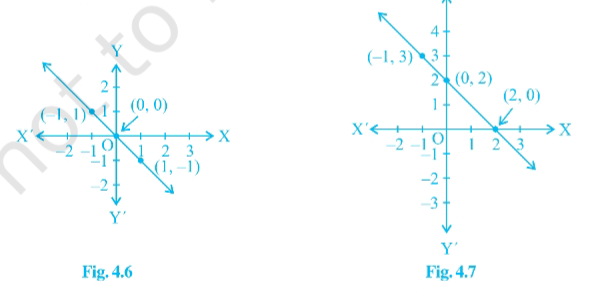
\includegraphics[width=\columnwidth]{chapters/9/figs/4.6-4.7.png}
\caption{Graph}
  \label{fig:4.6-4.7}
\end{figure}
\item If the work done by a body of a constant force is directly proportional 
to the distance travelled by the body,express this in the form of an equation
and draw the graph of the same by taking the varables and draw the graph of 
the same by taking the constant force as $5 units$.Also read from the graph the
work done when the distance travelled by the body is
\begin{enumerate}[label=(\roman*)]
\item $2$Units
\item $0$Unit
\end{enumerate}
\item Yamini and Fatima,two students of class IX of a school,together
 contributed \rupee~100 towards the prime minister's reief fund to help
 the earhquake victims.Write a linear equation which satisfies this data.
 (you may take their contributions  \rupee~x and \rupee~y.Draw the graph 
 of the same.
\item In Countries like USA and Canada temperature is measured in Celsius.
Here is a linear equation that converts Farenheit to celsius:
$F=\frac{9}{5}C+32$
\begin{enumerate}[label=(\roman*)]
\item Draw the graph of the linear equation above using Celsius for $x$
 axis and Farenheit for $y$ axis
\item If the temperature is $30\degree C$,what is the temperature in farenheight?
\item If the temperature is $95\degree F$,what is the temperature in celsius?
\item If the temperature is $0\degree C$.What is the temperature in Farenheit and if the temperature in celsius?
\item Is there a temperature Which is numerically same in both Farenheit and Celsius? If yes find it.
\end{enumerate}
\end{enumerate}

\section{10}
\subsection{Examples:-1-19 (10.3)}
\input{chapters/10/10.3.tex}
\subsection{10.3.1}
\input{chapters/10/10.3.1.tex}
\subsection{10.3.2}
\input{chapters/10/10.3.2.tex}
\subsection{10.3.3}
\begin{enumerate}
\item Solve the following pair of linear equations by the substitution method.
\begin{enumerate}[label=(\roman*)]    
	\item
	\begin{align}
   	 x+y=14 \\x-y=4
	\end{align}
    	\item 
	\begin{align}
	s-t=3
	\end{align}
	\item
	\begin{align}
    	3x-y=3\\ 9x-3y=9
	\end{align}
	\begin{align}   	
 	0.2x+0.3y=1.3\\ 0.4x+0.5y=23
	\end{align}
	\item     
	\begin{align}
	\sqrt{2x}+\sqrt{3y}=0\\ \sqrt{3x}-\sqrt{8y}=0
	\end{align}
	\item
	\begin{align}
    	\frac{3x}{2}-\frac{5y}{2}=-2\\ \frac{x}{3}+\frac{y}{2}=\frac{13}{6}
    	\end{align}
	\end{enumerate}
\item Solve $2x+3y=11$ and $2x+4y=-24$ and hence find the value of $m$ for which $y=mx+3$
\item Form the pair of linear equations for the following problems and find their solutions by the substitution method
    \begin{enumerate}[label=(\Roman*)]
    \item The difference between two numbers is $26$ and one number is three times the other. Find them.
    \item The larger of two supplementary angles exceeds the smaller by $18$ degrees. Find them.
    \item The coach of a cricket team buys $7$ balls and $6$ balls for \rupee~3800. Later, she buys $3$ bats and $5$ balls for \rupee~1750. Find the cost of each bat and each ball.
    \item The taxi charges in a city consist of a fixed charge together with the charges for the distance covered. For a distance of $10$ km, the charge paid is \rupee~105 and for a distance of $15$ km, the charge paid is \rupee~155. What are the fixed charges and the charge per km? How much does a person have to pay for travelling a distance of 25 km ? 
    \item A fraction becomes $\frac{9}{11}$ if $2$ is added to both the numerator and the denominator. If $3$ is added to both the numerator and the denominator, it becomes $\frac{5}{6}$. Find the fraction.
    \item Five years hence, the age of Jacob will be three times that of his son. Five years ago, Jacob's age was seven times that of his son. What are their present ages?
    \end{enumerate}
\end{enumerate}

\subsection{10.3.4}
\input{chapters/10/10.3.4.tex}
\subsection{10.3.5}
\input{chapters/10/10.3.5.tex}
\subsection{10.3.6}
\begin{enumerate}
\item Solve the following pair of equations by reducing them to a pair of linear equations:
\begin{enumerate}[label=(\roman*)]
\item
\begin{align}
\frac{1}{2x}+\frac{1}{3y}=2 \\ \frac{1}{3x}+\frac{1}{2y}=\frac{13}{6}
\end{align}
\item
\begin{align}
\frac{2}{\sqrt{x}}+\frac{3}{\sqrt{y}}=2\\
\frac{4}{\sqrt{x}}-\frac{9}{\sqrt{y}}=-1
\end{align}
\item
\begin{align}
\frac{4}{x}+3y=14\\ \frac{3}{x}-4y=23
\end{align}
\item
\begin{align}
\frac{5}{x-1}+\frac{1}{y-2}=2\\ \frac{6}{x-1}-\frac{3}{y-2}=1
\end{align}
\item
\begin{align}
\frac{7x-2y}{xy}=5\\ \frac{8x+7y}{xy}=15
\end{align}
\item
\begin{align}
6x+3y=6xy\\ 2x+4y=5xy
\end{align}
\item
\begin{align}
\frac{10}{x+y}+\frac{2}{x-y}=4\\ \frac{15}{x+y}-\frac{5}{x-y}=-2
\end{align}
\item
\begin{align}
\frac{1}{3x+y}+\frac{1}{3x-y}=\frac{3}{4}\\ \frac{1}{2(3x+y)}-\frac{1}{2(3x-y)}=\frac{-1}{8}
\end{align}
\end{enumerate}
\item Formulate the following problems as a pair of equations,and hence find their solutions:
\begin{enumerate}[label=(\roman*)]
\item Ritu can row downstream $20km$ in $2$ hours, and upstream $4km$ in $2$ hours. Find her speed of rowing in still water and the speed of the current.
\item $2$ women and $5$ men can together finish an embroidery work in $4$ days, while $3$ women and $6$ men can finish it in $3$ days. Find the time taken by $1$ women along to finish the work, and also that taken by $1$ men alone.
\item Roohi travels $300 km$ to her home partly by train and partly by bus. She takes $4$ hours if she travels $60km$ by train and the remaining by bus. If she travels $100km$ by train and the remaining by bus, she takes $10$ minutes longer. Find the speed of the train and the bus seperately.
\end{enumerate}
\end{enumerate}

\subsection{10.3.7}
\input{chapters/10/10.3.7.tex}
\chapter{Quadratic Equations}
\section{10}
\subsection{Examples:-1-18 (10.4)}                                               
\input{chapters/10/10.4.tex}
\subsection{10.4.1}
\input{chapters/10/10.4.1.tex}
\subsection{10.4.2}
\input{chapters/10/10.4.2.tex}
\subsection{10.4.3}
\input{chapters/10/10.4.3.tex}
\subsection{10.4.4}
\begin{enumerate}
\item Find the nature of the roots of the following quadratic equations. If real roots exist, find them:
\begin{enumerate}[label=(\roman*)]
\item $2x^2-3x+5=0$
\item $3x^2-4 sqrt 3x+4=0$
\item $2x^2-6x+3=0$
\end{enumerate}
\item Find the values of k for each of the following quadratic equations, so that they hav equal roots:
\begin{enumerate}[label=(\roman*)]
\item $2x^2=kx-3=0$
\item $kx(x-2)+6=0$
\end{enumerate}
\item Is it possible to design a rectangular mango grove whose length is twice its breadth, and the area is  $800m^2$? If so, find its length and breadth.
\item Is the following situation possible? If so, determine their present ages.
\\ The sum of the ages of the two friends is 20 years. Four years ago, the product of their ages in years was $48$.
\item Is it possible to design a rectangular park of perimeter 80m and area of $400m^2$. If so, find its length and breadth.
\end{enumerate}



\chapter{Coordinate Geometry}
\section{10}
\subsection{10.7.1}
\input{chapters/10/10.7.1.tex}
\subsection{10.7.2}
\input{chapters/10/10.7.2.tex}
\subsection{10.7.3}
\input{chapters/10/10.7.3.tex}
\subsection{10.7.4}
\input{chapters/10/10.7.4.tex}
\chapter{Straight Lines}
\section{11}
\subsection{11.10.1}
\input{chapters/11/11.10.1.tex}
\subsection{11.10.2}
\input{chapters/11/11.10.2.tex}
\subsection{11.10.3}
\input{chapters/11/11.10.3.tex}
\chapter{Trigonometry}
\section{Ratios}
\input{./chapters/trig/tri_geo_rt}
\section{The Baudhayana Theorem}
\input{./chapters/trig/tri_geo_baudh}
%
\section{Area of a Triangle}
\input{./chapters/trig/tri_geo_sincos}
\section{Angle Bisectors}
\input{./chapters/trig/ang.tex}
\section{Circumradius}
\input{./chapters/trig/tri_geo_cradius}
\section{Tangent}
\input{./chapters/trig/tangent}
\section{Identities}
\input{./chapters/trig/trig_id.tex}
\chapter{Analytic Geometry}
\section{Vectors}
\input{./chapters/coord/vector}
\section{Altitudes of a Triangle:Line Equation}
\input{./chapters/coord/tri_geo_alt}
\section{Circumcircle: Circle Equation}
\input{./chapters/coord/tri_geo_ccentre}
\section{Tangent}
\input{./chapters/coord/circ_geo_prop}
\chapter{Triangle}
\input{./chapters/exercises/tri_geo_exer}
\chapter{Quadrilateral}
\input{./chapters/exercises/quad_geo_exer}
%
\chapter{Circle}
\section{11}
\subsection{11.11.1}
In each of the following exercise \ref{prob:1} to \ref{prob:5}, find the equation of the circle with:
\begin{enumerate}[label=\arabic*.,ref=\thesubsection.\theenumi]
\item centre $(0,2)$ and radius $2$ \label{prob:1}
\item centre $(-2,3)$ and radius $4$
\item centre $\frac({1}{2},\frac{1}{4})$ and radius $\frac {1}{!2}$
\item centre $(1,1)$ and radius $2$
\item centre $(-a,-b)$ and radius $\sqrt{a^2-b^2}$  \label{prob:5}
\end{enumerate}
In each of the following exercise \ref{prob:6} to \ref{prob:9}, find the centre and radius of the circles
\begin{enumerate}[resume]
\item $(x-5)^2+(y-3)^2=36$ \label{prob:6}
\item $x^2+y^2-4x-8y-45=0$
\item $x^2+y^2-8x+10y-12=0$
\item $2x^2+2y^2-x=0$ \label{prob:9}
\end{enumerate}
\begin{enumerate}[resume]
\item Find the equation of the circle passing through the points $(4,1)$ and $(6,5)$ and whose centre is on the line $4x+y=16$.
\item Find the equation of the circle passing through the points $(2,3)$ and $(-1,1)$ and whose centre is on the line $x-3y-11=0$.
\item Find the equation of the circle with radius 5 whose centre lies on x-axis and passes through the point $(2,3)$.
\item Find the equation of the circle passing through $(0,0)$ and making intercepts $a$ and $b$ on the coordinate axes.
\item Find the equation of a circle with centre $(2,2)$ and passes through the point $(4,5)$.
\item Does the point $(-2.5,3.5)$ lie inside, outside or on the circle $x^2+y^2=25$.
\end{enumerate}



\input{./chapters/exercises/circ_geo_exer}
\chapter{Miscellaneous }
\input{./chapters/exercises/geo_misc}
\iffalse
%\include{ch02} 
\backmatter
\appendix
\chapter{Area of a Circle}
\input{./chapters/area/circ_geo_area}
\fi
%
%\chapter{Proofs}
%   \section{}
%\input{apps/defs.tex}

%  \section{}
%\input{apps/parab.tex}
%  \section{}
%\input{apps/nonparab.tex}
%		\section{}
%\input{apps/params.tex}
\latexprintindex

\end{document}

 

\item   Points $\vec{A}, \vec{B}, \vec{C}$ are defined to be collinear if 
		\begin{align}
			\rank{\myvec{1 & 1 & 1 \\ \vec{A}& \vec{B}&\vec{C}}} = 2
		\end{align}
Are the given points in
			\eqref{eq:tri-pts}
collinear?\\
\iffalse
\let\negmedspace\undefined
\let\negthickspace\undefined
\documentclass[journal,12pt,twocolumn]{IEEEtran}
\usepackage{cite}
\usepackage{amsmath,amssymb,amsfonts,amsthm}
\usepackage{algorithmic}
\usepackage{graphicx}
\usepackage{textcomp}
\usepackage{xcolor}
\usepackage{txfonts}
\usepackage{listings}
\usepackage{enumitem}
\usepackage{mathtools}
\usepackage{gensymb}
\usepackage[breaklinks=true]{hyperref}
\usepackage{tkz-euclide} % loads  TikZ and tkz-base
\usepackage{listings}
%\usepackage{gvv}
%
%\usepackage{setspace}
%\usepackage{gensymb}
%\doublespacing
%\singlespacing

%\usepackage{graphicx}
%\usepackage{amssymb}
%\usepackage{relsize}
%\usepackage[cmex10]{amsmath}
%\usepackage{amsthm}
%\interdisplaylinepenalty=2500
%\savesymbol{iint}
%\usepackage{txfonts}
%\restoresymbol{TXF}{iint}
%\usepackage{wasysym}
%\usepackage{amsthm}
%\usepackage{iithtlc}
%\usepackage{mathrsfs}
%\usepackage{txfonts}
%\usepackage{stfloats}
%\usepackage{bm}
%\usepackage{cite}
%\usepackage{cases}
%\usepackage{subfig}
%\usepackage{xtab}
%\usepackage{longtable}
%\usepackage{multirow}
%\usepackage{algorithm}
%\usepackage{algpseudocode}
%\usepackage{enumitem}
%\usepackage{mathtools}
%\usepackage{tikz}
%\usepackage{circuitikz}
%\usepackage{verbatim}
%\usepackage{tfrupee}
%\usepackage{stmaryrd}
%\usetkzobj{all}
%    \usepackage{color}                                            %%
%    \usepackage{array}                                            %%
%    \usepackage{longtable}                                        %%
%    \usepackage{calc}                                             %%
%    \usepackage{multirow}                                         %%
%    \usepackage{hhline}                                           %%
%    \usepackage{ifthen}                                           %%
  %optionally (for landscape tables embedded in another document): %%
%    \usepackage{lscape}     
%\usepackage{multicol}
%\usepackage{chngcntr}
%\usepackage{enumerate}

%\usepackage{wasysym}
%\documentclass[conference]{IEEEtran}
%\IEEEoverridecommandlockouts
% The preceding line is only needed to identify funding in the first footnote. If that is unneeded, please comment it out.

\newtheorem{theorem}{Theorem}[section]
\newtheorem{problem}{Problem}
\newtheorem{proposition}{Proposition}[section]
\newtheorem{lemma}{Lemma}[section]
\newtheorem{corollary}[theorem]{Corollary}
\newtheorem{example}{Example}[section]
\newtheorem{definition}[problem]{Definition}
%\newtheorem{thm}{Theorem}[section] 
%\newtheorem{defn}[thm]{Definition}
%\newtheorem{algorithm}{Algorithm}[section]
%\newtheorem{cor}{Corollary}
\newcommand{\BEQA}{\begin{eqnarray}}
\newcommand{\EEQA}{\end{eqnarray}}
\newcommand{\define}{\stackrel{\triangle}{=}}
\theoremstyle{remark}
\newtheorem{rem}{Remark}
\newcommand{\myvec}[1]{\ensuremath{\begin{pmatrix}#1\end{pmatrix}}}
\newcommand{\solution}{\noindent \textbf{Solution: }}
\providecommand{\brak}[1]{\ensuremath{\left(#1\right)}}
\providecommand{\rank}{\text{rank}}
\let\vec\mathbf

%\bibliographystyle{ieeetr}
\begin{document}
%

\bibliographystyle{IEEEtran}


\vspace{3cm}

\title{
%	\logo{
Assignment-1\\Probability and Random Processes
%	}
}
\author{ A.Rakesh Kumar EE22BTECH11005$^{*}$% <-this % stops a space
	%\thanks{*The author is with the Department
		%of Electrical Engineering, Indian Institute of Technology, Hyderabad
		%502285 India e-mail:  gadepall@iith.ac.in. All content in this manual is released under GNU GPL.  Free and open source.}
	
}	
%\title{
%	\logo{Matrix Analysis through Octave}{\begin{center}\includegraphics[scale=.24]{tlc}\end{center}}{}{HAMDSP}
%}


% paper title
% can use linebreaks \\ within to get better formatting as desired
%\title{Matrix Analysis through Octave}
%
%
% author names and IEEE memberships
% note positions of commas and nonbreaking spaces ( ~ ) LaTeX will not break
% a structure at a ~ so this keeps an author's name from being broken across
% two lines.
% use \thanks{} to gain access to the first footnote area
% a separate \thanks must be used for each paragraph as LaTeX2e's \thanks
% was not built to handle multiple paragraphs
%

%\author{<-this % stops a space
%\thanks{}}
%}
% note the % following the last \IEEEmembership and also \thanks - 
% these prevent an unwanted space from occurring between the last author name
% and the end of the author line. i.e., if you had this:
% 
% \author{....lastname \thanks{...} \thanks{...} }
%                     ^------------^------------^----Do not want these spaces!
%
% a space would be appended to the last name and could cause every name on that
% line to be shifted left slightly. This is one of those "LaTeX things". For
% instance, "\textbf{A} \textbf{B}" will typeset as "A B" not "AB". To get
% "AB" then you have to do: "\textbf{A}\textbf{B}"
% \thanks is no different in this regard, so shield the last } of each \thanks
% that ends a line with a % and do not let a space in before the next \thanks.
% Spaces after \IEEEmembership other than the last one are OK (and needed) as
% you are supposed to have spaces between the names. For what it is worth,
% this is a minor point as most people would not even notice if the said evil
% space somehow managed to creep in.



% The paper headers
%\markboth{Journal of \LaTeX\ Class Files,~Vol.~6, No.~1, January~2007}%
%{Shell \MakeLowercase{\textit{et al.}}: Bare Demo of IEEEtran.cls for Journals}
% The only time the second header will appear is for the odd numbered pages
% after the title page when using the twoside option.
% 
% *** Note that you probably will NOT want to include the author's ***
% *** name in the headers of peer review papers.                   ***
% You can use \ifCLASSOPTIONpeerreview for conditional compilation here if
% you desire.




% If you want to put a publisher's ID mark on the page you can do it like
% this:
%\IEEEpubid{0000--0000/00\$00.00~\copyright~2007 IEEE}
% Remember, if you use this you must call \IEEEpubidadjcol in the second
% column for its text to clear the IEEEpubid mark.



% make the title area
\maketitle

\newpage

%\tableofcontents

\bigskip

\renewcommand{\thefigure}{\theenumi}
\renewcommand{\thetable}{\theenumi}
%\renewcommand{\theequation}{\theenumi}

%\begin{abstract}
%%\boldmath
%In this letter, an algorithm for evaluating the exact analytical bit error rate  (BER)  for the piecewise linear (PL) combiner for  multiple relays is presented. Previous results were available only for upto three relays. The algorithm is unique in the sense that  the actual mathematical expressions, that are prohibitively large, need not be explicitly obtained. The diversity gain due to multiple relays is shown through plots of the analytical BER, well supported by simulations. 
%
%\end{abstract}
% IEEEtran.cls defaults to using nonbold math in the Abstract.
% This preserves the distinction between vectors and scalars. However,
% if the journal you are submitting to favors bold math in the abstract,
% then you can use LaTeX's standard command \boldmath at the very start
% of the abstract to achieve this. Many IEEE journals frown on math
% in the abstract anyway.

% Note that keywords are not normally used for peerreview papers.
%\begin{IEEEkeywords}
%Cooperative diversity, decode and forward, piecewise linear
%\end{IEEEkeywords}



% For peer review papers, you can put extra information on the cover
% page as needed:
% \ifCLASSOPTIONpeerreview
% \begin{center} \bfseries EDICS Category: 3-BBND \end{center}
% \fi
%
% For peerreview papers, this IEEEtran command inserts a page break and
% creates the second title. It will be ignored for other modes.
%\IEEEpeerreviewmaketitle
Question 1.1.3: Points A,B,C are defined to be collinear if
\begin{align} \rank \myvec{
1 & 1 & 1 \\
A & B & C
}=2 
\end{align}
Are the given points in (1.1) collinear?\\
\fi
\solution \\

Given, \begin{align}A=\myvec{
1 \\
-1
}, B=\myvec{
-4 \\
6
} , C=\myvec{
-3 \\
-5
}\\
\implies\myvec{
1 & 1 & 1 \\
A & B & C
}= \myvec{
1 & 1 & 1 \\
1 & -4 & -3 \\
-1 & 6 & -5}
\end{align}
Evaluating rank of the matrix using echelon form:
\begin{align}
\myvec{
1 & 1 & 1 \\
1 & -4 & -3 \\
-1 & 6 & -5}&\xleftrightarrow[]{R_2 \rightarrow R_2 - R_1}\myvec{
1 & 1 & 1 \\
0 & -5 & -4 \\
-1 & 6 & -5
}\\
\myvec{
1 & 1 & 1 \\
0 & -5 & -4 \\
-1 & 6 & -5
}&\xleftrightarrow[]{R_3 \rightarrow R_3 + R_2 - R_1}
\myvec{
1 & 1 & 1 \\
0 & -5 & -4 \\
0 & 0 & -10}
\end{align}
As the no.of non-zero rows are 3, the rank of the matrix is 3.\\
Hence,
\begin{align}\rank\myvec{
1 & 1 & 1 \\
A & B & C
}\neq 2 \end{align}
$\therefore$ The given points are not colinear.
\begin{figure}
\centering
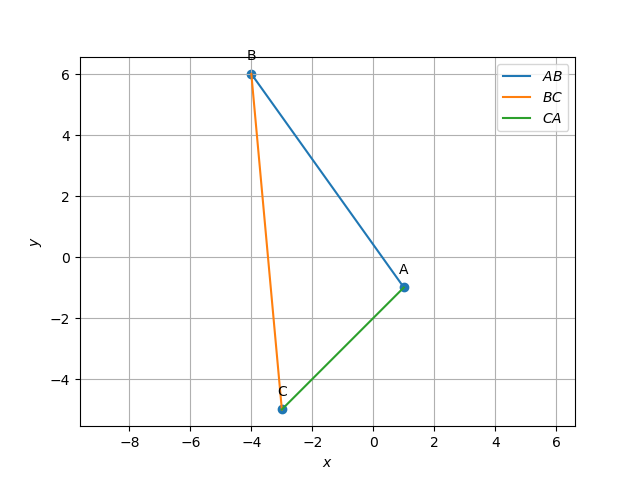
\includegraphics[width=\columnwidth]{figs/Figure_1}
\caption{$\vec{A}, \vec{B}, \vec{C}$ form a triangle.}
\label{fig:Figure_2}
\end{figure}

\item The parameteric form of the equation  of $AB$ is 
		\begin{align}
			\vec{x}=\vec{A}+k\vec{m}
		\end{align}
		where
		\begin{align}
\vec{m}=\vec{B}-\vec{A}
		\end{align}
is the direction vector of $AB$.
Find the parameteric equations of $AB, BC$ and $CA$.
\\
		%% Run LaTeX on this file several times to get Table of Contents,
%% cross-references, and citations.

\documentclass[11pt]{book}
\usepackage{gvv-book}
\usepackage{gvv}
%\usepackage{Wiley-AuthoringTemplate}
\usepackage[sectionbib,authoryear]{natbib}% for name-date citation comment the below line
%\usepackage[sectionbib,numbers]{natbib}% for numbered citation comment the above line

%%********************************************************************%%
%%       How many levels of section head would you like numbered?     %%
%% 0= no section numbers, 1= section, 2= section, 3= subsection %%
\setcounter{secnumdepth}{3}
%%********************************************************************%%
%%**********************************************************************%%
%%     How many levels of section head would you like to appear in the  %%
%%				Table of Contents?			%%
%% 0= chapter, 1= section, 2= section, 3= subsection titles.	%%
\setcounter{tocdepth}{2}
%%**********************************************************************%%

%\includeonly{ch01}
\makeindex

\begin{document}

\frontmatter
%%%%%%%%%%%%%%%%%%%%%%%%%%%%%%%%%%%%%%%%%%%%%%%%%%%%%%%%%%%%%%%%
%% Title Pages
%% Wiley will provide title and copyright page, but you can make
%% your own titlepages if you'd like anyway
%% Setting up title pages, type in the appropriate names here:

\booktitle{Geometry}

\subtitle{Through Algebra}

\AuAff{G. V. V. Sharma}


%% \\ will start a new line.
%% You may add \affil{} for affiliation, ie,
%\authors{Robert M. Groves\\
%\affil{Universitat de les Illes Balears}
%Floyd J. Fowler, Jr.\\
%\affil{University of New Mexico}
%}

%% Print Half Title and Title Page:
%\halftitlepage
\titlepage

%%%%%%%%%%%%%%%%%%%%%%%%%%%%%%%%%%%%%%%%%%%%%%%%%%%%%%%%%%%%%%%%
%% Copyright Page

\begin{copyrightpage}{2022}
%Title, etc
\end{copyrightpage}

% Note, you must use \ to start indented lines, ie,
% 
% \begin{copyrightpage}{2004}
% Survey Methodology / Robert M. Groves . . . [et al.].
% \       p. cm.---(Wiley series in survey methodology)
% \    ``Wiley-Interscience."
% \    Includes bibliographical references and index.
% \    ISBN 0-471-48348-6 (pbk.)
% \    1. Surveys---Methodology.  2. Social 
% \  sciences---Research---Statistical methods.  I. Groves, Robert M.  II. %
% Series.\\

% HA31.2.S873 2004
% 001.4'33---dc22                                             2004044064
% \end{copyrightpage}

%%%%%%%%%%%%%%%%%%%%%%%%%%%%%%%%%%%%%%%%%%%%%%%%%%%%%%%%%%%%%%%%
%% Only Dedication (optional) 

%\dedication{To my parents}

\tableofcontents

%\listoffigures %optional
%\listoftables  %optional

%% or Contributor Page for edited books
%% before \tableofcontents

%%%%%%%%%%%%%%%%%%%%%%%%%%%%%%%%%%%%%%%%%%%%%%%%%%%%%%%%%%%%%%%%
%  Contributors Page for Edited Book
%%%%%%%%%%%%%%%%%%%%%%%%%%%%%%%%%%%%%%%%%%%%%%%%%%%%%%%%%%%%%%%%

% If your book has chapters written by different authors,
% you'll need a Contributors page.

% Use \begin{contributors}...\end{contributors} and
% then enter each author with the \name{} command, followed
% by the affiliation information.

% \begin{contributors}
% \name{Masayki Abe,} Fujitsu Laboratories Ltd., Fujitsu Limited, Atsugi, Japan
%
% \name{L. A. Akers,} Center for Solid State Electronics Research, Arizona State University, Tempe, Arizona
%
% \name{G. H. Bernstein,} Department of Electrical and Computer Engineering, University of Notre Dame, Notre Dame, South Bend, Indiana; formerly of
% Center for Solid State Electronics Research, Arizona
% State University, Tempe, Arizona 
% \end{contributors}

%%%%%%%%%%%%%%%%%%%%%%%%%%%%%%%%%%%%%%%%%%%%%%%%%%%%%%%%%%%%%%%%
% Optional Foreword:

%\begin{foreword}
%\lipsum[1-2]
%\end{foreword}

%%%%%%%%%%%%%%%%%%%%%%%%%%%%%%%%%%%%%%%%%%%%%%%%%%%%%%%%%%%%%%%%
% Optional Preface:

%\begin{preface}
%\lipsum[1-1]
%\prefaceauthor{}
%\where{place\\
% date}
%\end{preface}

% ie,
% \begin{preface}
% This is an example preface.
% \prefaceauthor{R. K. Watts}
% \where{Durham, North Carolina\\
% September, 2004}

%%%%%%%%%%%%%%%%%%%%%%%%%%%%%%%%%%%%%%%%%%%%%%%%%%%%%%%%%%%%%%%%
% Optional Acknowledgments:

%\acknowledgments
%\lipsum[1-2]
%\authorinitials{I. R. S.}  

%%%%%%%%%%%%%%%%%%%%%%%%%%%%%%%%
%% Glossary Type of Environment:

% \begin{glossary}
% \term{<term>}{<description>}
% \end{glossary}

%%%%%%%%%%%%%%%%%%%%%%%%%%%%%%%%
%\begin{acronyms}
%\acro{ASTA}{Arrivals See Time Averages}
%\acro{BHCA}{Busy Hour Call Attempts}
%\acro{BR}{Bandwidth Reservation}
%\acro{b.u.}{bandwidth unit(s)}
%\acro{CAC}{Call / Connection Admission Control}
%\acro{CBP}{Call Blocking Probability(-ies)}
%\acro{CCS}{Centum Call Seconds}
%\acro{CDTM}{Connection Dependent Threshold Model}
%\acro{CS}{Complete Sharing}
%\acro{DiffServ}{Differentiated Services}
%\acro{EMLM}{Erlang Multirate Loss Model}
%\acro{erl}{The Erlang unit of traffic-load}
%\acro{FIFO}{First in - First out}
%\acro{GB}{Global balance}
%\acro{GoS}{Grade of Service}
%\acro{ICT}{Information and Communication Technology}
%\acro{IntServ}{Integrated Services}
%\acro{IP}{Internet Protocol}
%\acro{ITU-T}{International Telecommunication Unit -- Standardization sector}
%\acro{LB}{Local balance}
%\acro{LHS}{Left hand side}
%\acro{LIFO}{Last in - First out}
%\acro{MMPP}{Markov Modulated Poisson Process}
%\acro{MPLS}{Multiple Protocol Labeling Switching}
%\acro{MRM}{Multi-Retry Model}
%\acro{MTM}{Multi-Threshold Model}
%\acro{PASTA}{Poisson Arrivals See Time Averages}
%\acro{PDF}{Probability Distribution Function}
%\acro{pdf}{probability density function}
%\acro{PFS}{Product Form Solution}
%\acro{QoS}{Quality of Service}
%\acro{r.v.}{random variable(s)}
%\acro{RED}{random early detection}
%\acro{RHS}{Right hand side}
%\acro{RLA}{Reduced Load Approximation}
%\acro{SIRO}{service in random order}
%\acro{SRM}{Single-Retry Model}
%\acro{STM}{Single-Threshold Model}
%\acro{TCP}{Transport Control Protocol}
%\acro{TH}{Threshold(s)}
%\acro{UDP}{User Datagram Protocol}
%\end{acronyms}

\setcounter{page}{1}

\begin{introduction}
This book shows how to solve problems in geometry using trigonometry and coordinate geometry. 

\end{introduction}

\mainmatter

\chapter{Triangle}
Consider a triangle with vertices
		\begin{align}
			\label{eq:tri-pts}
			\vec{A} = \myvec{1 \\ -1},\,
			\vec{B} = \myvec{-4 \\ 6},\,
			\vec{C} = \myvec{-3 \\ -5}
		\end{align}
\section{Vectors}
%\renewcommand{\theequation}{\theenumi}
%\begin{enumerate}[label=\arabic*.,ref=\theenumi]
\begin{enumerate}[label=\thesection.\arabic*.,ref=\thesection.\theenumi]
\numberwithin{equation}{enumi}
\item The direction vector of $AB$ is defined as
		\begin{align}
			\vec{B}-
			\vec{A}
		\end{align}
Find the direction vectors of $AB, BC$ and $CA$.
\\
	\input{solutions/1/1/1/prob_1.tex}
	\item The length of side $BC$ is 
		\begin{align}
			\norm{\vec{B}-\vec{A}} \triangleq \sqrt{\brak{\vec{B}-\vec{A}}^{\top}{\vec{B}-\vec{A}}}
		\end{align}
		where
		\begin{align}
			\vec{A}^{\top}\triangleq\myvec{1 & -1}
		\end{align}
  \\		\input{solutions/1/1/2/main.tex}
\item   Points $\vec{A}, \vec{B}, \vec{C}$ are defined to be collinear if 
		\begin{align}
			\rank{\myvec{1 & 1 & 1 \\ \vec{A}& \vec{B}&\vec{C}}} = 2
		\end{align}
Are the given points in
			\eqref{eq:tri-pts}
collinear?\\
\input{solutions/1/1/3/main.tex}
\item The parameteric form of the equation  of $AB$ is 
		\begin{align}
			\vec{x}=\vec{A}+k\vec{m}
		\end{align}
		where
		\begin{align}
\vec{m}=\vec{B}-\vec{A}
		\end{align}
is the direction vector of $AB$.
Find the parameteric equations of $AB, BC$ and $CA$.
\\
		\input{solutions/1/1/4/main.tex}
\item The normal form of the equation of $AB$  is 
		\begin{align}
			\vec{n}^{\top}\brak{	\vec{x}-\vec{A}} = 0
		\end{align}
		where 
		\begin{align}
			\vec{n}^{\top}\vec{m}&=\vec{n}^{\top}\brak{\vec{B}-\vec{A}} = 0
			\\
			\text{or, } \vec{n}&=\myvec{0 & 1 \\ -1 & 0} \vec{m}
		\end{align}
Find the normal form of the equations of $AB, BC$ and $CA$.
\input{solutions/1/1/5/assign1.tex}
\input{solutions/1/1/5a/assignment1.tex}
\input{solutions/1/1/5c/main.tex}
\item The area of $\triangle ABC$ is defined as
		\begin{align}
			\frac{1}{2}\norm{{\brak{\vec{A}-\vec{B}}\times {\vec{A}-\vec{C}}}}
		\end{align}
		where
		\begin{align}
			\vec{A}\times\vec{B} \triangleq \mydet{1 & -4 \\-1 & 6}
		\end{align}
		Find the area of $\triangle ABC$.\\
  		\input{solutions/1/1/6/main.tex}
	\item Find the angles $A, B, C$ if 
    \label{prop:angle2d}
  \begin{align}
    \label{eq:angle2d}
			\cos A \triangleq 
\frac{\brak{\vec{B}-\vec{A}}^{\top}{\vec{C}-\vec{A}}}{\norm{\vec{B}-\vec{A}}\norm{\vec{C}-\vec{A}}}
  \end{align}\\
  	\input{solutions/1/1/7/main.tex}
\end{enumerate}

\section{Median}
%\renewcommand{\theequation}{\theenumi}
%\begin{enumerate}[label=\arabic*.,ref=\theenumi]
\begin{enumerate}[label=\thesection.\arabic*.,ref=\thesection.\theenumi]
\numberwithin{equation}{enumi}
\item If $\vec{D}$ divides $BC$ in the ratio $k : 1$,
		\begin{align}
			\vec{D}= \frac{k\vec{C}+\vec{B}}{k+1}
		\end{align}
		Find the mid points $\vec{D}, \vec{E}, \vec{F}$ of the sides $BC, CA$ and $AB$ respectively.
		\\
			\input{solutions/1/2/1/main.tex} 
	\item Find the equations of $AD, BE$ and $CF$.
	\item Find the intersection $\vec{G}$ of $BE$ and $CF$.
	\item Verify that 
		\begin{align}
			\frac{BG}{GE} = 
			\frac{CG}{GF} =
			\frac{AG}{GD} =2 
		\end{align}
	\item Show that $\vec{A}, \vec{G}$ and $\vec{D}$ are collinear.
	\item Verify that 
		\begin{align}
			\vec{G}=\frac{\vec{A}+\vec{B}+\vec{C}}{3}
		\end{align}
			$\vec{G}$ is known as the {\em centroid} of $\triangle ABC$.
   \\
		\input{solutions/1/2/6/main.tex}
	\item Verify that 
		\begin{align}
\vec{A}-\vec{F}=\vec{E}-\vec{D}
		\end{align}
		The quadrilateral $AFDE$ is defined to be a parallelogram.
\end{enumerate}

\section{Altitude}
%\renewcommand{\theequation}{\theenumi}
%\begin{enumerate}[label=\arabic*.,ref=\theenumi]
\begin{enumerate}[label=\thesection.\arabic*.,ref=\thesection.\theenumi]
\numberwithin{equation}{enumi}
\item $\vec{D}_1$ is a point on $BC$ such that
		\begin{align}
			AD_1 \perp BC
		\end{align}
		and $AD_1$ is defined to be the altitude. 
		Find the normal vector of $AD_1$.
  \\
		\input{solutions/1/3/1/main.tex}
	\item Find the equation of $AD_1$.

	\item Find the equations of the altitudes $BE_1$ and $CF_1$ to the sides $AC$ and $AB$ respectively. 
	\item Find the intersection $\vec{H}$ of $BE_1$ and $CF_1$.
	\item Verify that 
		\begin{align}
			\brak{\vec{A}-\vec{H}}^{\top}\brak{\vec{B}-\vec{C}} = 0
		\end{align}
  \\
  	\input{solutions/1/3/5/main.tex}
\end{enumerate}

\section{Perpendicular Bisector}
%\renewcommand{\theequation}{\theenumi}
%\begin{enumerate}[label=\arabic*.,ref=\theenumi]
\begin{enumerate}[label=\thesection.\arabic*.,ref=\thesection.\theenumi]
\numberwithin{equation}{enumi}

\item The equation of the perpendicular bisector of $BC$ is
		\begin{align}
			\label{eq:tri-perp-bisect}
			\brak{\vec{x}-\frac{\vec{B}+\vec{C}}{2}}\brak{\vec{B}-\vec{C}} = 0
		\end{align}
		Substitute numerical values and find the equations of the perpendicular bisectors of $AB, BC$ and $CA$.
	\\	\input{solutions/1/4/1/q1.4.1.tex}
	\item Find the intersection $\vec{O}$ of the perpendicular bisectors of $AB$ and $AC$.
 \\
 \input{solutions/1/4/2/main.tex}
	\item Verify that $\vec{O}$ satisfies
			\eqref{eq:tri-perp-bisect}.
$\vec{O}$ is known as the circumcentre.\\
   \input{solutions/1/4/3/main.tex}
		\item Verify that 
		\begin{align}
			OA = OB = OC 
		\end{align}
  \\
  \input{solutions/1/4/4/main.tex}
  \input{solutions/1/4/4(1)/main.tex}
	\item Draw the circle with centre at $\vec{O}$ and radius 
		\begin{align}
			R = OA
		\end{align}
		This is known as the {\em circumradius}. 
  \\  \input{solutions/1/4/5/assignment2.tex}
	\item Verify that 
		\begin{align}
			\angle BOC = 2\angle BAC.
		\end{align}\\
  \input{solutions/1/4/6/Q_1.4.6.tex}
	\item Let 
		\begin{align}
			\vec{P} = \myvec{\cos \theta & -\sin \theta \\ \sin \theta & \cos \theta}
		\end{align}
		Find $\theta$ if 
		\begin{align}
			\vec{C}-\vec{O}=\vec{P}\brak{\vec{A}-\vec{O}}
		\end{align}
\end{enumerate}

\section{Angle Bisector}
%\renewcommand{\theequation}{\theenumi}
%\begin{enumerate}[label=\arabic*.,ref=\theenumi]
\begin{enumerate}[label=\thesection.\arabic*.,ref=\thesection.\theenumi]
\numberwithin{equation}{enumi}
\item Suppose the equations $AB, BC$ and $CA$ are respectively given by 
		\begin{align}
			\label{eq:tri-sides}
			\vec{n}_i^{\top}\vec{x}=c_i \quad i = 1, 2, 3 
		\end{align}
		The equations of the respective angle bisectors are then given by 
		\begin{align}
			\frac{\vec{n}_i^{\top}\vec{x}-c_i}{\norm{\vec{n}_i}}
		=
	\pm	\frac{\vec{n}_j^{\top}\vec{x}-c_j}{\norm{\vec{n}_j}}
\quad i \ne j
		\end{align}
		Substitute numerical values and find the equations of the angle bisectors of $A, B$ and $C$.
	\\
		%\input{solutions/1/5/1/Assignment_1.tex}
  \input{solutions/1/5/1(1)/main.tex}
	\item Find the intersection $\vec{I}$ of the angle bisectors of $B$ and $C$.
 \\
		\input{solutions/1/5/2/main.tex}
	\item Using 
    \eqref{eq:angle2d}
verify that 
		\begin{align}
			\angle BAI = \angle CAI.
		\end{align}
	\item Find the distance from $\vec{I}$ to $BC$.  \\
        \input{solutions/1/5/4/main.tex}
	\item Repeat the above exercise for the sides $AB$ and $AC$.
	\item This distance is known as the {\em inradius} $r$.
	\item Draw a circle with center $\vec{I}$ and radius $r$.  $\vec{I}$ is known as the {\em incentre}.
	\item The equation of the {\em incircle} is given by 
		\begin{align}
			\norm{\vec{x}-\vec{I}}^2 = r^2
		\end{align}
		Find the parameteric equation of $BC$ and use it to verify that $BC$ intersects the incircle at exactly one point $\vec{D}_3$.  $BC$ is defined to be a {\em tangent} to the incircle.  $\vec{D}_3$ is defined to be {\em point of contact}.
	\\
		\input{solutions/1/5/8/main.tex}
  \item Find the other points of contact $\vec{E}_3$ and $\vec{F}_3$.
	\item Verify that 
		\begin{align}
			AE_3 = AF_3=m, BD_3 = BF_3=n, CD_3 = CE_3=p.
		\end{align}
	\item Obtain $m,n,p$ in terms of $a,b,c$, the sides of the triangle using a matrix equation.  Obtain the numerical values.
 \\
 		\input{solutions/1/5/11/main.tex}
\end{enumerate}

%
\chapter{Linear Equations}
\section{9}
\subsection{9.3.3}
\input{chapters/9/9.3.3.tex}
\subsection{9.4.1}
\begin{enumerate}[label=\arabic*.,ref=\theenumi]
\item The cost of a notebook is twice the cost of a pen.Write a linear
equation in two variables to represent this statement.
(Take the Cost of a notebook to be $x$ and that of a pen to be
$y$).
\item Express the following linear equation in the form $ax+by+c=0$
and indicate the values of $a,b$ and $c$ in each case:
%\begin{enumerate}
\begin{enumerate}[label=(\roman*),ref=\theenumi]
\item $2x+3y=9.3\overline{5}$
\item $x-\frac{y}{5}-10=10$
\item $-2x+3y=6$
\item $ x=3y$
\item $2x=-5y$
\item $3x+2=0$
\item $y-2=0$
\item $5=2x$
\end{enumerate}
\end{enumerate}

\subsection{9.4.2}
\input{chapters/9/9.4.2.tex}
\subsection{9.4.3}
\begin{enumerate}[label=\arabic*.,ref=\theenumi]
\item Draw the graph of each of the following linear equations in two variables:
\begin{enumerate}[label=(\roman*),ref=\theenumi]
\item $x+y=4$
\item $x-y=2$
\item $y=3x$
\item $3=2x+y$
\end{enumerate}
\item Give the equations of two lines passing through (2,14).How many more such lines are there and 
why?
\item If the point(3,4) lies on the graph of the equation $3y=ax+7$ find the value of a
\item The taxi fare in the city is as follows:for te first kilometre,the fare is \rupee~8 and for the 
subsquent distance is \rupee~5 per km.Taking the distance Covered as $x$ km and total fare as
\rupee~y.Write a linear equation for this information,and draw its graph.
\item From the choices given below,choose the equation whose graphs are given Fig 4.6 Fig 4.7
\\
For fig-4.6 
\begin{enumerate}[label=(\roman*)]
\item $y=x$
\item $x+y=0$
\item $y=2x$
\item $2+3y=7x$
\end{enumerate} 
For fig-4.7 
\begin{enumerate}[label=(\roman*)]
\item $y=x+2$
\item $y=x-2$
\item $y=-x+2$
\item $x+2y=6$
\end{enumerate}
\begin{figure}[ht]
\centering
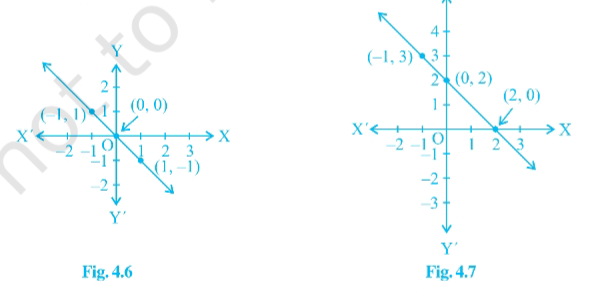
\includegraphics[width=\columnwidth]{chapters/9/figs/4.6-4.7.png}
\caption{Graph}
  \label{fig:4.6-4.7}
\end{figure}
\item If the work done by a body of a constant force is directly proportional 
to the distance travelled by the body,express this in the form of an equation
and draw the graph of the same by taking the varables and draw the graph of 
the same by taking the constant force as $5 units$.Also read from the graph the
work done when the distance travelled by the body is
\begin{enumerate}[label=(\roman*)]
\item $2$Units
\item $0$Unit
\end{enumerate}
\item Yamini and Fatima,two students of class IX of a school,together
 contributed \rupee~100 towards the prime minister's reief fund to help
 the earhquake victims.Write a linear equation which satisfies this data.
 (you may take their contributions  \rupee~x and \rupee~y.Draw the graph 
 of the same.
\item In Countries like USA and Canada temperature is measured in Celsius.
Here is a linear equation that converts Farenheit to celsius:
$F=\frac{9}{5}C+32$
\begin{enumerate}[label=(\roman*)]
\item Draw the graph of the linear equation above using Celsius for $x$
 axis and Farenheit for $y$ axis
\item If the temperature is $30\degree C$,what is the temperature in farenheight?
\item If the temperature is $95\degree F$,what is the temperature in celsius?
\item If the temperature is $0\degree C$.What is the temperature in Farenheit and if the temperature in celsius?
\item Is there a temperature Which is numerically same in both Farenheit and Celsius? If yes find it.
\end{enumerate}
\end{enumerate}

\section{10}
\subsection{Examples:-1-19 (10.3)}
\input{chapters/10/10.3.tex}
\subsection{10.3.1}
\input{chapters/10/10.3.1.tex}
\subsection{10.3.2}
\input{chapters/10/10.3.2.tex}
\subsection{10.3.3}
\begin{enumerate}
\item Solve the following pair of linear equations by the substitution method.
\begin{enumerate}[label=(\roman*)]    
	\item
	\begin{align}
   	 x+y=14 \\x-y=4
	\end{align}
    	\item 
	\begin{align}
	s-t=3
	\end{align}
	\item
	\begin{align}
    	3x-y=3\\ 9x-3y=9
	\end{align}
	\begin{align}   	
 	0.2x+0.3y=1.3\\ 0.4x+0.5y=23
	\end{align}
	\item     
	\begin{align}
	\sqrt{2x}+\sqrt{3y}=0\\ \sqrt{3x}-\sqrt{8y}=0
	\end{align}
	\item
	\begin{align}
    	\frac{3x}{2}-\frac{5y}{2}=-2\\ \frac{x}{3}+\frac{y}{2}=\frac{13}{6}
    	\end{align}
	\end{enumerate}
\item Solve $2x+3y=11$ and $2x+4y=-24$ and hence find the value of $m$ for which $y=mx+3$
\item Form the pair of linear equations for the following problems and find their solutions by the substitution method
    \begin{enumerate}[label=(\Roman*)]
    \item The difference between two numbers is $26$ and one number is three times the other. Find them.
    \item The larger of two supplementary angles exceeds the smaller by $18$ degrees. Find them.
    \item The coach of a cricket team buys $7$ balls and $6$ balls for \rupee~3800. Later, she buys $3$ bats and $5$ balls for \rupee~1750. Find the cost of each bat and each ball.
    \item The taxi charges in a city consist of a fixed charge together with the charges for the distance covered. For a distance of $10$ km, the charge paid is \rupee~105 and for a distance of $15$ km, the charge paid is \rupee~155. What are the fixed charges and the charge per km? How much does a person have to pay for travelling a distance of 25 km ? 
    \item A fraction becomes $\frac{9}{11}$ if $2$ is added to both the numerator and the denominator. If $3$ is added to both the numerator and the denominator, it becomes $\frac{5}{6}$. Find the fraction.
    \item Five years hence, the age of Jacob will be three times that of his son. Five years ago, Jacob's age was seven times that of his son. What are their present ages?
    \end{enumerate}
\end{enumerate}

\subsection{10.3.4}
\input{chapters/10/10.3.4.tex}
\subsection{10.3.5}
\input{chapters/10/10.3.5.tex}
\subsection{10.3.6}
\begin{enumerate}
\item Solve the following pair of equations by reducing them to a pair of linear equations:
\begin{enumerate}[label=(\roman*)]
\item
\begin{align}
\frac{1}{2x}+\frac{1}{3y}=2 \\ \frac{1}{3x}+\frac{1}{2y}=\frac{13}{6}
\end{align}
\item
\begin{align}
\frac{2}{\sqrt{x}}+\frac{3}{\sqrt{y}}=2\\
\frac{4}{\sqrt{x}}-\frac{9}{\sqrt{y}}=-1
\end{align}
\item
\begin{align}
\frac{4}{x}+3y=14\\ \frac{3}{x}-4y=23
\end{align}
\item
\begin{align}
\frac{5}{x-1}+\frac{1}{y-2}=2\\ \frac{6}{x-1}-\frac{3}{y-2}=1
\end{align}
\item
\begin{align}
\frac{7x-2y}{xy}=5\\ \frac{8x+7y}{xy}=15
\end{align}
\item
\begin{align}
6x+3y=6xy\\ 2x+4y=5xy
\end{align}
\item
\begin{align}
\frac{10}{x+y}+\frac{2}{x-y}=4\\ \frac{15}{x+y}-\frac{5}{x-y}=-2
\end{align}
\item
\begin{align}
\frac{1}{3x+y}+\frac{1}{3x-y}=\frac{3}{4}\\ \frac{1}{2(3x+y)}-\frac{1}{2(3x-y)}=\frac{-1}{8}
\end{align}
\end{enumerate}
\item Formulate the following problems as a pair of equations,and hence find their solutions:
\begin{enumerate}[label=(\roman*)]
\item Ritu can row downstream $20km$ in $2$ hours, and upstream $4km$ in $2$ hours. Find her speed of rowing in still water and the speed of the current.
\item $2$ women and $5$ men can together finish an embroidery work in $4$ days, while $3$ women and $6$ men can finish it in $3$ days. Find the time taken by $1$ women along to finish the work, and also that taken by $1$ men alone.
\item Roohi travels $300 km$ to her home partly by train and partly by bus. She takes $4$ hours if she travels $60km$ by train and the remaining by bus. If she travels $100km$ by train and the remaining by bus, she takes $10$ minutes longer. Find the speed of the train and the bus seperately.
\end{enumerate}
\end{enumerate}

\subsection{10.3.7}
\input{chapters/10/10.3.7.tex}
\chapter{Quadratic Equations}
\section{10}
\subsection{Examples:-1-18 (10.4)}                                               
\input{chapters/10/10.4.tex}
\subsection{10.4.1}
\input{chapters/10/10.4.1.tex}
\subsection{10.4.2}
\input{chapters/10/10.4.2.tex}
\subsection{10.4.3}
\input{chapters/10/10.4.3.tex}
\subsection{10.4.4}
\begin{enumerate}
\item Find the nature of the roots of the following quadratic equations. If real roots exist, find them:
\begin{enumerate}[label=(\roman*)]
\item $2x^2-3x+5=0$
\item $3x^2-4 sqrt 3x+4=0$
\item $2x^2-6x+3=0$
\end{enumerate}
\item Find the values of k for each of the following quadratic equations, so that they hav equal roots:
\begin{enumerate}[label=(\roman*)]
\item $2x^2=kx-3=0$
\item $kx(x-2)+6=0$
\end{enumerate}
\item Is it possible to design a rectangular mango grove whose length is twice its breadth, and the area is  $800m^2$? If so, find its length and breadth.
\item Is the following situation possible? If so, determine their present ages.
\\ The sum of the ages of the two friends is 20 years. Four years ago, the product of their ages in years was $48$.
\item Is it possible to design a rectangular park of perimeter 80m and area of $400m^2$. If so, find its length and breadth.
\end{enumerate}



\chapter{Coordinate Geometry}
\section{10}
\subsection{10.7.1}
\input{chapters/10/10.7.1.tex}
\subsection{10.7.2}
\input{chapters/10/10.7.2.tex}
\subsection{10.7.3}
\input{chapters/10/10.7.3.tex}
\subsection{10.7.4}
\input{chapters/10/10.7.4.tex}
\chapter{Straight Lines}
\section{11}
\subsection{11.10.1}
\input{chapters/11/11.10.1.tex}
\subsection{11.10.2}
\input{chapters/11/11.10.2.tex}
\subsection{11.10.3}
\input{chapters/11/11.10.3.tex}
\chapter{Trigonometry}
\section{Ratios}
\input{./chapters/trig/tri_geo_rt}
\section{The Baudhayana Theorem}
\input{./chapters/trig/tri_geo_baudh}
%
\section{Area of a Triangle}
\input{./chapters/trig/tri_geo_sincos}
\section{Angle Bisectors}
\input{./chapters/trig/ang.tex}
\section{Circumradius}
\input{./chapters/trig/tri_geo_cradius}
\section{Tangent}
\input{./chapters/trig/tangent}
\section{Identities}
\input{./chapters/trig/trig_id.tex}
\chapter{Analytic Geometry}
\section{Vectors}
\input{./chapters/coord/vector}
\section{Altitudes of a Triangle:Line Equation}
\input{./chapters/coord/tri_geo_alt}
\section{Circumcircle: Circle Equation}
\input{./chapters/coord/tri_geo_ccentre}
\section{Tangent}
\input{./chapters/coord/circ_geo_prop}
\chapter{Triangle}
\input{./chapters/exercises/tri_geo_exer}
\chapter{Quadrilateral}
\input{./chapters/exercises/quad_geo_exer}
%
\chapter{Circle}
\section{11}
\subsection{11.11.1}
In each of the following exercise \ref{prob:1} to \ref{prob:5}, find the equation of the circle with:
\begin{enumerate}[label=\arabic*.,ref=\thesubsection.\theenumi]
\item centre $(0,2)$ and radius $2$ \label{prob:1}
\item centre $(-2,3)$ and radius $4$
\item centre $\frac({1}{2},\frac{1}{4})$ and radius $\frac {1}{!2}$
\item centre $(1,1)$ and radius $2$
\item centre $(-a,-b)$ and radius $\sqrt{a^2-b^2}$  \label{prob:5}
\end{enumerate}
In each of the following exercise \ref{prob:6} to \ref{prob:9}, find the centre and radius of the circles
\begin{enumerate}[resume]
\item $(x-5)^2+(y-3)^2=36$ \label{prob:6}
\item $x^2+y^2-4x-8y-45=0$
\item $x^2+y^2-8x+10y-12=0$
\item $2x^2+2y^2-x=0$ \label{prob:9}
\end{enumerate}
\begin{enumerate}[resume]
\item Find the equation of the circle passing through the points $(4,1)$ and $(6,5)$ and whose centre is on the line $4x+y=16$.
\item Find the equation of the circle passing through the points $(2,3)$ and $(-1,1)$ and whose centre is on the line $x-3y-11=0$.
\item Find the equation of the circle with radius 5 whose centre lies on x-axis and passes through the point $(2,3)$.
\item Find the equation of the circle passing through $(0,0)$ and making intercepts $a$ and $b$ on the coordinate axes.
\item Find the equation of a circle with centre $(2,2)$ and passes through the point $(4,5)$.
\item Does the point $(-2.5,3.5)$ lie inside, outside or on the circle $x^2+y^2=25$.
\end{enumerate}



\input{./chapters/exercises/circ_geo_exer}
\chapter{Miscellaneous }
\input{./chapters/exercises/geo_misc}
\iffalse
%\include{ch02} 
\backmatter
\appendix
\chapter{Area of a Circle}
\input{./chapters/area/circ_geo_area}
\fi
%
%\chapter{Proofs}
%   \section{}
%\input{apps/defs.tex}

%  \section{}
%\input{apps/parab.tex}
%  \section{}
%\input{apps/nonparab.tex}
%		\section{}
%\input{apps/params.tex}
\latexprintindex

\end{document}

 

\item The normal form of the equation of $AB$  is 
		\begin{align}
			\vec{n}^{\top}\brak{	\vec{x}-\vec{A}} = 0
		\end{align}
		where 
		\begin{align}
			\vec{n}^{\top}\vec{m}&=\vec{n}^{\top}\brak{\vec{B}-\vec{A}} = 0
			\\
			\text{or, } \vec{n}&=\myvec{0 & 1 \\ -1 & 0} \vec{m}
		\end{align}
Find the normal form of the equations of $AB, BC$ and $CA$.
\input{solutions/1/1/5/assign1.tex}
\input{solutions/1/1/5a/assignment1.tex}
\iffalse
\documentclass[12pt]{article}
\usepackage{amsmath}
\usepackage{graphicx}
\begin{document}

\providecommand{\pr}[1]{\ensuremath{\Pr\left(#1\right)}}
\providecommand{\prt}[2]{\ensuremath{p_{#1}^{\left(#2\right)} }}        % own macro for this question
\providecommand{\qfunc}[1]{\ensuremath{Q\left(#1\right)}}
\providecommand{\sbrak}[1]{\ensuremath{{}\left[#1\right]}}
\providecommand{\lsbrak}[1]{\ensuremath{{}\left[#1\right.}}
\providecommand{\rsbrak}[1]{\ensuremath{{}\left.#1\right]}}
\providecommand{\brak}[1]{\ensuremath{\left(#1\right)}}
\providecommand{\lbrak}[1]{\ensuremath{\left(#1\right.}}
\providecommand{\rbrak}[1]{\ensuremath{\left.#1\right)}}
\providecommand{\cbrak}[1]{\ensuremath{\left\{#1\right\}}}
\providecommand{\lcbrak}[1]{\ensuremath{\left\{#1\right.}}
\providecommand{\rcbrak}[1]{\ensuremath{\left.#1\right\}}}
\newcommand{\sgn}{\mathop{\mathrm{sgn}}}
\providecommand{\abs}[1]{\left\vert#1\right\vert}
\providecommand{\res}[1]{\Res\displaylimits_{#1}} 
\providecommand{\norm}[1]{\left\lVert#1\right\rVert}
%\providecommand{\norm}[1]{\lVert#1\rVert}
\providecommand{\mtx}[1]{\mathbf{#1}}
\providecommand{\mean}[1]{E\left[ #1 \right]}
\providecommand{\cond}[2]{#1\middle|#2}
\providecommand{\fourier}{\overset{\mathcal{F}}{ \rightleftharpoons}}
\newenvironment{amatrix}[1]{%
  \left(\begin{array}{@{}*{#1}{c}|c@{}}
}{%
  \end{array}\right)
}
%\providecommand{\hilbert}{\overset{\mathcal{H}}{ \rightleftharpoons}}
%\providecommand{\system}{\overset{\mathcal{H}}{ \longleftrightarrow}}
	%\newcommand{\solution}[2]{\textbf{Solution:}{#1}}
\newcommand{\solution}{\noindent \textbf{Solution: }}
\newcommand{\cosec}{\,\text{cosec}\,}
\providecommand{\dec}[2]{\ensuremath{\overset{#1}{\underset{#2}{\gtrless}}}}
\newcommand{\myvec}[1]{\ensuremath{\begin{pmatrix}#1\end{pmatrix}}}
\newcommand{\mydet}[1]{\ensuremath{\begin{vmatrix}#1\end{vmatrix}}}
\newcommand{\myaugvec}[2]{\ensuremath{\begin{amatrix}{#1}#2\end{amatrix}}}
\providecommand{\rank}{\text{rank}}
\providecommand{\pr}[1]{\ensuremath{\Pr\left(#1\right)}}
\providecommand{\qfunc}[1]{\ensuremath{Q\left(#1\right)}}
	\newcommand*{\permcomb}[4][0mu]{{{}^{#3}\mkern#1#2_{#4}}}
\newcommand*{\perm}[1][-3mu]{\permcomb[#1]{P}}
\newcommand*{\comb}[1][-1mu]{\permcomb[#1]{C}}
\providecommand{\qfunc}[1]{\ensuremath{Q\left(#1\right)}}
\providecommand{\gauss}[2]{\mathcal{N}\ensuremath{\left(#1,#2\right)}}
\providecommand{\diff}[2]{\ensuremath{\frac{d{#1}}{d{#2}}}}
\providecommand{\myceil}[1]{\left \lceil #1 \right \rceil }
\newcommand\figref{Fig.~\ref}
\newcommand\tabref{Table~\ref}
\newcommand{\sinc}{\,\text{sinc}\,}
\newcommand{\rect}{\,\text{rect}\,}
%%
%	%\newcommand{\solution}[2]{\textbf{Solution:}{#1}}
%\newcommand{\solution}{\noindent \textbf{Solution: }}
%\newcommand{\cosec}{\,\text{cosec}\,}
%\numberwithin{equation}{section}
%\numberwithin{equation}{subsection}
%\numberwithin{problem}{section}
%\numberwithin{definition}{section}
%\makeatletter
%\@addtoreset{figure}{problem}
%\makeatother

%\let\StandardTheFigure\thefigure
\let\vec\mathbf
Q 1.1.5. The normal form of the equation of $AB$ is
\begin{align}
\vec{n}^{\top}\myvec{\vec{x}-\vec{A}} = 0
\end{align}
where
\begin{align}
\vec{n}^{\top}\vec{m} &= \vec{n}^{\top}\myvec{\vec{B} - \vec{A}} = 0 \\
\text{or, } \vec{n} &= \myvec{0&1 \\ -1&0} \vec{m}
\end{align}
Find the normal form of the equations of $AB$, $BC$ and $CA$.\\
\fi
\solution
The direction vector for $CA$ vector is given by
\begin{align}
\vec{m} &= \vec{A} - \vec{C}\\
&= \myvec{1 \\ -1} - \myvec{-3 \\ -5}\\
&= \myvec{4 \\ 4}
\end{align}
Now, normal vector is given by
\begin{align}
\vec{n} &= \myvec{0&1 \\ -1&0}\vec{m}\\
&= \myvec{0&1 \\ -1&0}\myvec{4 \\ 4}\\
&= \myvec{4 \\ -4}\\
\implies \vec{n}^{\top} &= \myvec{4&-4}
\end{align}
Therefore, normal form of equation of line $CA$ is
\begin{align}
\vec{n}^{\top}(\vec{x} - \vec{C}) &= 0 \\
\implies \vec{n}^{\top}{\vec{x}} - \vec{n}^{\top}{\vec{C}} &= 0 \\
\implies \vec{n}^{\top}{\vec{x}} &= \vec{n}^{\top}{\vec{C}} \\
\implies \myvec{4&-4}{\vec{x}} &= \myvec{4&-4}\myvec{-3 \\ -5} \\
&= -12 + 20 \\
&= 8 
\end{align}
Hence, the required equation of $CA$ is
\begin{align}
\label{eq:CA}
\myvec{4&-4}{\vec{x}} &= 8 
\end{align}
\begin{figure}
\centering
\includegraphics[width=\columnwidth]{solutions/1/1/5/figs/fig.png}
\caption{Line CA generated using python}
\label{fig: line_CA_py}
\end{figure}

\item The area of $\triangle ABC$ is defined as
		\begin{align}
			\frac{1}{2}\norm{{\brak{\vec{A}-\vec{B}}\times {\vec{A}-\vec{C}}}}
		\end{align}
		where
		\begin{align}
			\vec{A}\times\vec{B} \triangleq \mydet{1 & -4 \\-1 & 6}
		\end{align}
		Find the area of $\triangle ABC$.\\
  		%% Run LaTeX on this file several times to get Table of Contents,
%% cross-references, and citations.

\documentclass[11pt]{book}
\usepackage{gvv-book}
\usepackage{gvv}
%\usepackage{Wiley-AuthoringTemplate}
\usepackage[sectionbib,authoryear]{natbib}% for name-date citation comment the below line
%\usepackage[sectionbib,numbers]{natbib}% for numbered citation comment the above line

%%********************************************************************%%
%%       How many levels of section head would you like numbered?     %%
%% 0= no section numbers, 1= section, 2= section, 3= subsection %%
\setcounter{secnumdepth}{3}
%%********************************************************************%%
%%**********************************************************************%%
%%     How many levels of section head would you like to appear in the  %%
%%				Table of Contents?			%%
%% 0= chapter, 1= section, 2= section, 3= subsection titles.	%%
\setcounter{tocdepth}{2}
%%**********************************************************************%%

%\includeonly{ch01}
\makeindex

\begin{document}

\frontmatter
%%%%%%%%%%%%%%%%%%%%%%%%%%%%%%%%%%%%%%%%%%%%%%%%%%%%%%%%%%%%%%%%
%% Title Pages
%% Wiley will provide title and copyright page, but you can make
%% your own titlepages if you'd like anyway
%% Setting up title pages, type in the appropriate names here:

\booktitle{Geometry}

\subtitle{Through Algebra}

\AuAff{G. V. V. Sharma}


%% \\ will start a new line.
%% You may add \affil{} for affiliation, ie,
%\authors{Robert M. Groves\\
%\affil{Universitat de les Illes Balears}
%Floyd J. Fowler, Jr.\\
%\affil{University of New Mexico}
%}

%% Print Half Title and Title Page:
%\halftitlepage
\titlepage

%%%%%%%%%%%%%%%%%%%%%%%%%%%%%%%%%%%%%%%%%%%%%%%%%%%%%%%%%%%%%%%%
%% Copyright Page

\begin{copyrightpage}{2022}
%Title, etc
\end{copyrightpage}

% Note, you must use \ to start indented lines, ie,
% 
% \begin{copyrightpage}{2004}
% Survey Methodology / Robert M. Groves . . . [et al.].
% \       p. cm.---(Wiley series in survey methodology)
% \    ``Wiley-Interscience."
% \    Includes bibliographical references and index.
% \    ISBN 0-471-48348-6 (pbk.)
% \    1. Surveys---Methodology.  2. Social 
% \  sciences---Research---Statistical methods.  I. Groves, Robert M.  II. %
% Series.\\

% HA31.2.S873 2004
% 001.4'33---dc22                                             2004044064
% \end{copyrightpage}

%%%%%%%%%%%%%%%%%%%%%%%%%%%%%%%%%%%%%%%%%%%%%%%%%%%%%%%%%%%%%%%%
%% Only Dedication (optional) 

%\dedication{To my parents}

\tableofcontents

%\listoffigures %optional
%\listoftables  %optional

%% or Contributor Page for edited books
%% before \tableofcontents

%%%%%%%%%%%%%%%%%%%%%%%%%%%%%%%%%%%%%%%%%%%%%%%%%%%%%%%%%%%%%%%%
%  Contributors Page for Edited Book
%%%%%%%%%%%%%%%%%%%%%%%%%%%%%%%%%%%%%%%%%%%%%%%%%%%%%%%%%%%%%%%%

% If your book has chapters written by different authors,
% you'll need a Contributors page.

% Use \begin{contributors}...\end{contributors} and
% then enter each author with the \name{} command, followed
% by the affiliation information.

% \begin{contributors}
% \name{Masayki Abe,} Fujitsu Laboratories Ltd., Fujitsu Limited, Atsugi, Japan
%
% \name{L. A. Akers,} Center for Solid State Electronics Research, Arizona State University, Tempe, Arizona
%
% \name{G. H. Bernstein,} Department of Electrical and Computer Engineering, University of Notre Dame, Notre Dame, South Bend, Indiana; formerly of
% Center for Solid State Electronics Research, Arizona
% State University, Tempe, Arizona 
% \end{contributors}

%%%%%%%%%%%%%%%%%%%%%%%%%%%%%%%%%%%%%%%%%%%%%%%%%%%%%%%%%%%%%%%%
% Optional Foreword:

%\begin{foreword}
%\lipsum[1-2]
%\end{foreword}

%%%%%%%%%%%%%%%%%%%%%%%%%%%%%%%%%%%%%%%%%%%%%%%%%%%%%%%%%%%%%%%%
% Optional Preface:

%\begin{preface}
%\lipsum[1-1]
%\prefaceauthor{}
%\where{place\\
% date}
%\end{preface}

% ie,
% \begin{preface}
% This is an example preface.
% \prefaceauthor{R. K. Watts}
% \where{Durham, North Carolina\\
% September, 2004}

%%%%%%%%%%%%%%%%%%%%%%%%%%%%%%%%%%%%%%%%%%%%%%%%%%%%%%%%%%%%%%%%
% Optional Acknowledgments:

%\acknowledgments
%\lipsum[1-2]
%\authorinitials{I. R. S.}  

%%%%%%%%%%%%%%%%%%%%%%%%%%%%%%%%
%% Glossary Type of Environment:

% \begin{glossary}
% \term{<term>}{<description>}
% \end{glossary}

%%%%%%%%%%%%%%%%%%%%%%%%%%%%%%%%
%\begin{acronyms}
%\acro{ASTA}{Arrivals See Time Averages}
%\acro{BHCA}{Busy Hour Call Attempts}
%\acro{BR}{Bandwidth Reservation}
%\acro{b.u.}{bandwidth unit(s)}
%\acro{CAC}{Call / Connection Admission Control}
%\acro{CBP}{Call Blocking Probability(-ies)}
%\acro{CCS}{Centum Call Seconds}
%\acro{CDTM}{Connection Dependent Threshold Model}
%\acro{CS}{Complete Sharing}
%\acro{DiffServ}{Differentiated Services}
%\acro{EMLM}{Erlang Multirate Loss Model}
%\acro{erl}{The Erlang unit of traffic-load}
%\acro{FIFO}{First in - First out}
%\acro{GB}{Global balance}
%\acro{GoS}{Grade of Service}
%\acro{ICT}{Information and Communication Technology}
%\acro{IntServ}{Integrated Services}
%\acro{IP}{Internet Protocol}
%\acro{ITU-T}{International Telecommunication Unit -- Standardization sector}
%\acro{LB}{Local balance}
%\acro{LHS}{Left hand side}
%\acro{LIFO}{Last in - First out}
%\acro{MMPP}{Markov Modulated Poisson Process}
%\acro{MPLS}{Multiple Protocol Labeling Switching}
%\acro{MRM}{Multi-Retry Model}
%\acro{MTM}{Multi-Threshold Model}
%\acro{PASTA}{Poisson Arrivals See Time Averages}
%\acro{PDF}{Probability Distribution Function}
%\acro{pdf}{probability density function}
%\acro{PFS}{Product Form Solution}
%\acro{QoS}{Quality of Service}
%\acro{r.v.}{random variable(s)}
%\acro{RED}{random early detection}
%\acro{RHS}{Right hand side}
%\acro{RLA}{Reduced Load Approximation}
%\acro{SIRO}{service in random order}
%\acro{SRM}{Single-Retry Model}
%\acro{STM}{Single-Threshold Model}
%\acro{TCP}{Transport Control Protocol}
%\acro{TH}{Threshold(s)}
%\acro{UDP}{User Datagram Protocol}
%\end{acronyms}

\setcounter{page}{1}

\begin{introduction}
This book shows how to solve problems in geometry using trigonometry and coordinate geometry. 

\end{introduction}

\mainmatter

\chapter{Triangle}
Consider a triangle with vertices
		\begin{align}
			\label{eq:tri-pts}
			\vec{A} = \myvec{1 \\ -1},\,
			\vec{B} = \myvec{-4 \\ 6},\,
			\vec{C} = \myvec{-3 \\ -5}
		\end{align}
\section{Vectors}
%\renewcommand{\theequation}{\theenumi}
%\begin{enumerate}[label=\arabic*.,ref=\theenumi]
\begin{enumerate}[label=\thesection.\arabic*.,ref=\thesection.\theenumi]
\numberwithin{equation}{enumi}
\item The direction vector of $AB$ is defined as
		\begin{align}
			\vec{B}-
			\vec{A}
		\end{align}
Find the direction vectors of $AB, BC$ and $CA$.
\\
	\input{solutions/1/1/1/prob_1.tex}
	\item The length of side $BC$ is 
		\begin{align}
			\norm{\vec{B}-\vec{A}} \triangleq \sqrt{\brak{\vec{B}-\vec{A}}^{\top}{\vec{B}-\vec{A}}}
		\end{align}
		where
		\begin{align}
			\vec{A}^{\top}\triangleq\myvec{1 & -1}
		\end{align}
  \\		\input{solutions/1/1/2/main.tex}
\item   Points $\vec{A}, \vec{B}, \vec{C}$ are defined to be collinear if 
		\begin{align}
			\rank{\myvec{1 & 1 & 1 \\ \vec{A}& \vec{B}&\vec{C}}} = 2
		\end{align}
Are the given points in
			\eqref{eq:tri-pts}
collinear?\\
\input{solutions/1/1/3/main.tex}
\item The parameteric form of the equation  of $AB$ is 
		\begin{align}
			\vec{x}=\vec{A}+k\vec{m}
		\end{align}
		where
		\begin{align}
\vec{m}=\vec{B}-\vec{A}
		\end{align}
is the direction vector of $AB$.
Find the parameteric equations of $AB, BC$ and $CA$.
\\
		\input{solutions/1/1/4/main.tex}
\item The normal form of the equation of $AB$  is 
		\begin{align}
			\vec{n}^{\top}\brak{	\vec{x}-\vec{A}} = 0
		\end{align}
		where 
		\begin{align}
			\vec{n}^{\top}\vec{m}&=\vec{n}^{\top}\brak{\vec{B}-\vec{A}} = 0
			\\
			\text{or, } \vec{n}&=\myvec{0 & 1 \\ -1 & 0} \vec{m}
		\end{align}
Find the normal form of the equations of $AB, BC$ and $CA$.
\input{solutions/1/1/5/assign1.tex}
\input{solutions/1/1/5a/assignment1.tex}
\input{solutions/1/1/5c/main.tex}
\item The area of $\triangle ABC$ is defined as
		\begin{align}
			\frac{1}{2}\norm{{\brak{\vec{A}-\vec{B}}\times {\vec{A}-\vec{C}}}}
		\end{align}
		where
		\begin{align}
			\vec{A}\times\vec{B} \triangleq \mydet{1 & -4 \\-1 & 6}
		\end{align}
		Find the area of $\triangle ABC$.\\
  		\input{solutions/1/1/6/main.tex}
	\item Find the angles $A, B, C$ if 
    \label{prop:angle2d}
  \begin{align}
    \label{eq:angle2d}
			\cos A \triangleq 
\frac{\brak{\vec{B}-\vec{A}}^{\top}{\vec{C}-\vec{A}}}{\norm{\vec{B}-\vec{A}}\norm{\vec{C}-\vec{A}}}
  \end{align}\\
  	\input{solutions/1/1/7/main.tex}
\end{enumerate}

\section{Median}
%\renewcommand{\theequation}{\theenumi}
%\begin{enumerate}[label=\arabic*.,ref=\theenumi]
\begin{enumerate}[label=\thesection.\arabic*.,ref=\thesection.\theenumi]
\numberwithin{equation}{enumi}
\item If $\vec{D}$ divides $BC$ in the ratio $k : 1$,
		\begin{align}
			\vec{D}= \frac{k\vec{C}+\vec{B}}{k+1}
		\end{align}
		Find the mid points $\vec{D}, \vec{E}, \vec{F}$ of the sides $BC, CA$ and $AB$ respectively.
		\\
			\input{solutions/1/2/1/main.tex} 
	\item Find the equations of $AD, BE$ and $CF$.
	\item Find the intersection $\vec{G}$ of $BE$ and $CF$.
	\item Verify that 
		\begin{align}
			\frac{BG}{GE} = 
			\frac{CG}{GF} =
			\frac{AG}{GD} =2 
		\end{align}
	\item Show that $\vec{A}, \vec{G}$ and $\vec{D}$ are collinear.
	\item Verify that 
		\begin{align}
			\vec{G}=\frac{\vec{A}+\vec{B}+\vec{C}}{3}
		\end{align}
			$\vec{G}$ is known as the {\em centroid} of $\triangle ABC$.
   \\
		\input{solutions/1/2/6/main.tex}
	\item Verify that 
		\begin{align}
\vec{A}-\vec{F}=\vec{E}-\vec{D}
		\end{align}
		The quadrilateral $AFDE$ is defined to be a parallelogram.
\end{enumerate}

\section{Altitude}
%\renewcommand{\theequation}{\theenumi}
%\begin{enumerate}[label=\arabic*.,ref=\theenumi]
\begin{enumerate}[label=\thesection.\arabic*.,ref=\thesection.\theenumi]
\numberwithin{equation}{enumi}
\item $\vec{D}_1$ is a point on $BC$ such that
		\begin{align}
			AD_1 \perp BC
		\end{align}
		and $AD_1$ is defined to be the altitude. 
		Find the normal vector of $AD_1$.
  \\
		\input{solutions/1/3/1/main.tex}
	\item Find the equation of $AD_1$.

	\item Find the equations of the altitudes $BE_1$ and $CF_1$ to the sides $AC$ and $AB$ respectively. 
	\item Find the intersection $\vec{H}$ of $BE_1$ and $CF_1$.
	\item Verify that 
		\begin{align}
			\brak{\vec{A}-\vec{H}}^{\top}\brak{\vec{B}-\vec{C}} = 0
		\end{align}
  \\
  	\input{solutions/1/3/5/main.tex}
\end{enumerate}

\section{Perpendicular Bisector}
%\renewcommand{\theequation}{\theenumi}
%\begin{enumerate}[label=\arabic*.,ref=\theenumi]
\begin{enumerate}[label=\thesection.\arabic*.,ref=\thesection.\theenumi]
\numberwithin{equation}{enumi}

\item The equation of the perpendicular bisector of $BC$ is
		\begin{align}
			\label{eq:tri-perp-bisect}
			\brak{\vec{x}-\frac{\vec{B}+\vec{C}}{2}}\brak{\vec{B}-\vec{C}} = 0
		\end{align}
		Substitute numerical values and find the equations of the perpendicular bisectors of $AB, BC$ and $CA$.
	\\	\input{solutions/1/4/1/q1.4.1.tex}
	\item Find the intersection $\vec{O}$ of the perpendicular bisectors of $AB$ and $AC$.
 \\
 \input{solutions/1/4/2/main.tex}
	\item Verify that $\vec{O}$ satisfies
			\eqref{eq:tri-perp-bisect}.
$\vec{O}$ is known as the circumcentre.\\
   \input{solutions/1/4/3/main.tex}
		\item Verify that 
		\begin{align}
			OA = OB = OC 
		\end{align}
  \\
  \input{solutions/1/4/4/main.tex}
  \input{solutions/1/4/4(1)/main.tex}
	\item Draw the circle with centre at $\vec{O}$ and radius 
		\begin{align}
			R = OA
		\end{align}
		This is known as the {\em circumradius}. 
  \\  \input{solutions/1/4/5/assignment2.tex}
	\item Verify that 
		\begin{align}
			\angle BOC = 2\angle BAC.
		\end{align}\\
  \input{solutions/1/4/6/Q_1.4.6.tex}
	\item Let 
		\begin{align}
			\vec{P} = \myvec{\cos \theta & -\sin \theta \\ \sin \theta & \cos \theta}
		\end{align}
		Find $\theta$ if 
		\begin{align}
			\vec{C}-\vec{O}=\vec{P}\brak{\vec{A}-\vec{O}}
		\end{align}
\end{enumerate}

\section{Angle Bisector}
%\renewcommand{\theequation}{\theenumi}
%\begin{enumerate}[label=\arabic*.,ref=\theenumi]
\begin{enumerate}[label=\thesection.\arabic*.,ref=\thesection.\theenumi]
\numberwithin{equation}{enumi}
\item Suppose the equations $AB, BC$ and $CA$ are respectively given by 
		\begin{align}
			\label{eq:tri-sides}
			\vec{n}_i^{\top}\vec{x}=c_i \quad i = 1, 2, 3 
		\end{align}
		The equations of the respective angle bisectors are then given by 
		\begin{align}
			\frac{\vec{n}_i^{\top}\vec{x}-c_i}{\norm{\vec{n}_i}}
		=
	\pm	\frac{\vec{n}_j^{\top}\vec{x}-c_j}{\norm{\vec{n}_j}}
\quad i \ne j
		\end{align}
		Substitute numerical values and find the equations of the angle bisectors of $A, B$ and $C$.
	\\
		%\input{solutions/1/5/1/Assignment_1.tex}
  \input{solutions/1/5/1(1)/main.tex}
	\item Find the intersection $\vec{I}$ of the angle bisectors of $B$ and $C$.
 \\
		\input{solutions/1/5/2/main.tex}
	\item Using 
    \eqref{eq:angle2d}
verify that 
		\begin{align}
			\angle BAI = \angle CAI.
		\end{align}
	\item Find the distance from $\vec{I}$ to $BC$.  \\
        \input{solutions/1/5/4/main.tex}
	\item Repeat the above exercise for the sides $AB$ and $AC$.
	\item This distance is known as the {\em inradius} $r$.
	\item Draw a circle with center $\vec{I}$ and radius $r$.  $\vec{I}$ is known as the {\em incentre}.
	\item The equation of the {\em incircle} is given by 
		\begin{align}
			\norm{\vec{x}-\vec{I}}^2 = r^2
		\end{align}
		Find the parameteric equation of $BC$ and use it to verify that $BC$ intersects the incircle at exactly one point $\vec{D}_3$.  $BC$ is defined to be a {\em tangent} to the incircle.  $\vec{D}_3$ is defined to be {\em point of contact}.
	\\
		\input{solutions/1/5/8/main.tex}
  \item Find the other points of contact $\vec{E}_3$ and $\vec{F}_3$.
	\item Verify that 
		\begin{align}
			AE_3 = AF_3=m, BD_3 = BF_3=n, CD_3 = CE_3=p.
		\end{align}
	\item Obtain $m,n,p$ in terms of $a,b,c$, the sides of the triangle using a matrix equation.  Obtain the numerical values.
 \\
 		\input{solutions/1/5/11/main.tex}
\end{enumerate}

%
\chapter{Linear Equations}
\section{9}
\subsection{9.3.3}
\input{chapters/9/9.3.3.tex}
\subsection{9.4.1}
\begin{enumerate}[label=\arabic*.,ref=\theenumi]
\item The cost of a notebook is twice the cost of a pen.Write a linear
equation in two variables to represent this statement.
(Take the Cost of a notebook to be $x$ and that of a pen to be
$y$).
\item Express the following linear equation in the form $ax+by+c=0$
and indicate the values of $a,b$ and $c$ in each case:
%\begin{enumerate}
\begin{enumerate}[label=(\roman*),ref=\theenumi]
\item $2x+3y=9.3\overline{5}$
\item $x-\frac{y}{5}-10=10$
\item $-2x+3y=6$
\item $ x=3y$
\item $2x=-5y$
\item $3x+2=0$
\item $y-2=0$
\item $5=2x$
\end{enumerate}
\end{enumerate}

\subsection{9.4.2}
\input{chapters/9/9.4.2.tex}
\subsection{9.4.3}
\begin{enumerate}[label=\arabic*.,ref=\theenumi]
\item Draw the graph of each of the following linear equations in two variables:
\begin{enumerate}[label=(\roman*),ref=\theenumi]
\item $x+y=4$
\item $x-y=2$
\item $y=3x$
\item $3=2x+y$
\end{enumerate}
\item Give the equations of two lines passing through (2,14).How many more such lines are there and 
why?
\item If the point(3,4) lies on the graph of the equation $3y=ax+7$ find the value of a
\item The taxi fare in the city is as follows:for te first kilometre,the fare is \rupee~8 and for the 
subsquent distance is \rupee~5 per km.Taking the distance Covered as $x$ km and total fare as
\rupee~y.Write a linear equation for this information,and draw its graph.
\item From the choices given below,choose the equation whose graphs are given Fig 4.6 Fig 4.7
\\
For fig-4.6 
\begin{enumerate}[label=(\roman*)]
\item $y=x$
\item $x+y=0$
\item $y=2x$
\item $2+3y=7x$
\end{enumerate} 
For fig-4.7 
\begin{enumerate}[label=(\roman*)]
\item $y=x+2$
\item $y=x-2$
\item $y=-x+2$
\item $x+2y=6$
\end{enumerate}
\begin{figure}[ht]
\centering
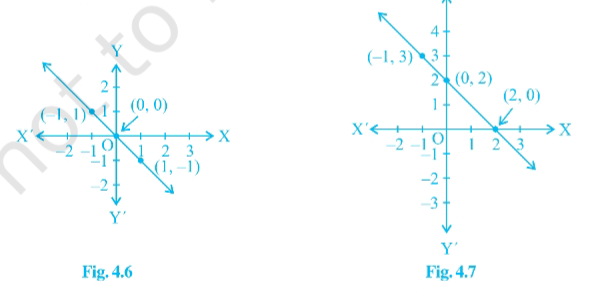
\includegraphics[width=\columnwidth]{chapters/9/figs/4.6-4.7.png}
\caption{Graph}
  \label{fig:4.6-4.7}
\end{figure}
\item If the work done by a body of a constant force is directly proportional 
to the distance travelled by the body,express this in the form of an equation
and draw the graph of the same by taking the varables and draw the graph of 
the same by taking the constant force as $5 units$.Also read from the graph the
work done when the distance travelled by the body is
\begin{enumerate}[label=(\roman*)]
\item $2$Units
\item $0$Unit
\end{enumerate}
\item Yamini and Fatima,two students of class IX of a school,together
 contributed \rupee~100 towards the prime minister's reief fund to help
 the earhquake victims.Write a linear equation which satisfies this data.
 (you may take their contributions  \rupee~x and \rupee~y.Draw the graph 
 of the same.
\item In Countries like USA and Canada temperature is measured in Celsius.
Here is a linear equation that converts Farenheit to celsius:
$F=\frac{9}{5}C+32$
\begin{enumerate}[label=(\roman*)]
\item Draw the graph of the linear equation above using Celsius for $x$
 axis and Farenheit for $y$ axis
\item If the temperature is $30\degree C$,what is the temperature in farenheight?
\item If the temperature is $95\degree F$,what is the temperature in celsius?
\item If the temperature is $0\degree C$.What is the temperature in Farenheit and if the temperature in celsius?
\item Is there a temperature Which is numerically same in both Farenheit and Celsius? If yes find it.
\end{enumerate}
\end{enumerate}

\section{10}
\subsection{Examples:-1-19 (10.3)}
\input{chapters/10/10.3.tex}
\subsection{10.3.1}
\input{chapters/10/10.3.1.tex}
\subsection{10.3.2}
\input{chapters/10/10.3.2.tex}
\subsection{10.3.3}
\begin{enumerate}
\item Solve the following pair of linear equations by the substitution method.
\begin{enumerate}[label=(\roman*)]    
	\item
	\begin{align}
   	 x+y=14 \\x-y=4
	\end{align}
    	\item 
	\begin{align}
	s-t=3
	\end{align}
	\item
	\begin{align}
    	3x-y=3\\ 9x-3y=9
	\end{align}
	\begin{align}   	
 	0.2x+0.3y=1.3\\ 0.4x+0.5y=23
	\end{align}
	\item     
	\begin{align}
	\sqrt{2x}+\sqrt{3y}=0\\ \sqrt{3x}-\sqrt{8y}=0
	\end{align}
	\item
	\begin{align}
    	\frac{3x}{2}-\frac{5y}{2}=-2\\ \frac{x}{3}+\frac{y}{2}=\frac{13}{6}
    	\end{align}
	\end{enumerate}
\item Solve $2x+3y=11$ and $2x+4y=-24$ and hence find the value of $m$ for which $y=mx+3$
\item Form the pair of linear equations for the following problems and find their solutions by the substitution method
    \begin{enumerate}[label=(\Roman*)]
    \item The difference between two numbers is $26$ and one number is three times the other. Find them.
    \item The larger of two supplementary angles exceeds the smaller by $18$ degrees. Find them.
    \item The coach of a cricket team buys $7$ balls and $6$ balls for \rupee~3800. Later, she buys $3$ bats and $5$ balls for \rupee~1750. Find the cost of each bat and each ball.
    \item The taxi charges in a city consist of a fixed charge together with the charges for the distance covered. For a distance of $10$ km, the charge paid is \rupee~105 and for a distance of $15$ km, the charge paid is \rupee~155. What are the fixed charges and the charge per km? How much does a person have to pay for travelling a distance of 25 km ? 
    \item A fraction becomes $\frac{9}{11}$ if $2$ is added to both the numerator and the denominator. If $3$ is added to both the numerator and the denominator, it becomes $\frac{5}{6}$. Find the fraction.
    \item Five years hence, the age of Jacob will be three times that of his son. Five years ago, Jacob's age was seven times that of his son. What are their present ages?
    \end{enumerate}
\end{enumerate}

\subsection{10.3.4}
\input{chapters/10/10.3.4.tex}
\subsection{10.3.5}
\input{chapters/10/10.3.5.tex}
\subsection{10.3.6}
\begin{enumerate}
\item Solve the following pair of equations by reducing them to a pair of linear equations:
\begin{enumerate}[label=(\roman*)]
\item
\begin{align}
\frac{1}{2x}+\frac{1}{3y}=2 \\ \frac{1}{3x}+\frac{1}{2y}=\frac{13}{6}
\end{align}
\item
\begin{align}
\frac{2}{\sqrt{x}}+\frac{3}{\sqrt{y}}=2\\
\frac{4}{\sqrt{x}}-\frac{9}{\sqrt{y}}=-1
\end{align}
\item
\begin{align}
\frac{4}{x}+3y=14\\ \frac{3}{x}-4y=23
\end{align}
\item
\begin{align}
\frac{5}{x-1}+\frac{1}{y-2}=2\\ \frac{6}{x-1}-\frac{3}{y-2}=1
\end{align}
\item
\begin{align}
\frac{7x-2y}{xy}=5\\ \frac{8x+7y}{xy}=15
\end{align}
\item
\begin{align}
6x+3y=6xy\\ 2x+4y=5xy
\end{align}
\item
\begin{align}
\frac{10}{x+y}+\frac{2}{x-y}=4\\ \frac{15}{x+y}-\frac{5}{x-y}=-2
\end{align}
\item
\begin{align}
\frac{1}{3x+y}+\frac{1}{3x-y}=\frac{3}{4}\\ \frac{1}{2(3x+y)}-\frac{1}{2(3x-y)}=\frac{-1}{8}
\end{align}
\end{enumerate}
\item Formulate the following problems as a pair of equations,and hence find their solutions:
\begin{enumerate}[label=(\roman*)]
\item Ritu can row downstream $20km$ in $2$ hours, and upstream $4km$ in $2$ hours. Find her speed of rowing in still water and the speed of the current.
\item $2$ women and $5$ men can together finish an embroidery work in $4$ days, while $3$ women and $6$ men can finish it in $3$ days. Find the time taken by $1$ women along to finish the work, and also that taken by $1$ men alone.
\item Roohi travels $300 km$ to her home partly by train and partly by bus. She takes $4$ hours if she travels $60km$ by train and the remaining by bus. If she travels $100km$ by train and the remaining by bus, she takes $10$ minutes longer. Find the speed of the train and the bus seperately.
\end{enumerate}
\end{enumerate}

\subsection{10.3.7}
\input{chapters/10/10.3.7.tex}
\chapter{Quadratic Equations}
\section{10}
\subsection{Examples:-1-18 (10.4)}                                               
\input{chapters/10/10.4.tex}
\subsection{10.4.1}
\input{chapters/10/10.4.1.tex}
\subsection{10.4.2}
\input{chapters/10/10.4.2.tex}
\subsection{10.4.3}
\input{chapters/10/10.4.3.tex}
\subsection{10.4.4}
\begin{enumerate}
\item Find the nature of the roots of the following quadratic equations. If real roots exist, find them:
\begin{enumerate}[label=(\roman*)]
\item $2x^2-3x+5=0$
\item $3x^2-4 sqrt 3x+4=0$
\item $2x^2-6x+3=0$
\end{enumerate}
\item Find the values of k for each of the following quadratic equations, so that they hav equal roots:
\begin{enumerate}[label=(\roman*)]
\item $2x^2=kx-3=0$
\item $kx(x-2)+6=0$
\end{enumerate}
\item Is it possible to design a rectangular mango grove whose length is twice its breadth, and the area is  $800m^2$? If so, find its length and breadth.
\item Is the following situation possible? If so, determine their present ages.
\\ The sum of the ages of the two friends is 20 years. Four years ago, the product of their ages in years was $48$.
\item Is it possible to design a rectangular park of perimeter 80m and area of $400m^2$. If so, find its length and breadth.
\end{enumerate}



\chapter{Coordinate Geometry}
\section{10}
\subsection{10.7.1}
\input{chapters/10/10.7.1.tex}
\subsection{10.7.2}
\input{chapters/10/10.7.2.tex}
\subsection{10.7.3}
\input{chapters/10/10.7.3.tex}
\subsection{10.7.4}
\input{chapters/10/10.7.4.tex}
\chapter{Straight Lines}
\section{11}
\subsection{11.10.1}
\input{chapters/11/11.10.1.tex}
\subsection{11.10.2}
\input{chapters/11/11.10.2.tex}
\subsection{11.10.3}
\input{chapters/11/11.10.3.tex}
\chapter{Trigonometry}
\section{Ratios}
\input{./chapters/trig/tri_geo_rt}
\section{The Baudhayana Theorem}
\input{./chapters/trig/tri_geo_baudh}
%
\section{Area of a Triangle}
\input{./chapters/trig/tri_geo_sincos}
\section{Angle Bisectors}
\input{./chapters/trig/ang.tex}
\section{Circumradius}
\input{./chapters/trig/tri_geo_cradius}
\section{Tangent}
\input{./chapters/trig/tangent}
\section{Identities}
\input{./chapters/trig/trig_id.tex}
\chapter{Analytic Geometry}
\section{Vectors}
\input{./chapters/coord/vector}
\section{Altitudes of a Triangle:Line Equation}
\input{./chapters/coord/tri_geo_alt}
\section{Circumcircle: Circle Equation}
\input{./chapters/coord/tri_geo_ccentre}
\section{Tangent}
\input{./chapters/coord/circ_geo_prop}
\chapter{Triangle}
\input{./chapters/exercises/tri_geo_exer}
\chapter{Quadrilateral}
\input{./chapters/exercises/quad_geo_exer}
%
\chapter{Circle}
\section{11}
\subsection{11.11.1}
In each of the following exercise \ref{prob:1} to \ref{prob:5}, find the equation of the circle with:
\begin{enumerate}[label=\arabic*.,ref=\thesubsection.\theenumi]
\item centre $(0,2)$ and radius $2$ \label{prob:1}
\item centre $(-2,3)$ and radius $4$
\item centre $\frac({1}{2},\frac{1}{4})$ and radius $\frac {1}{!2}$
\item centre $(1,1)$ and radius $2$
\item centre $(-a,-b)$ and radius $\sqrt{a^2-b^2}$  \label{prob:5}
\end{enumerate}
In each of the following exercise \ref{prob:6} to \ref{prob:9}, find the centre and radius of the circles
\begin{enumerate}[resume]
\item $(x-5)^2+(y-3)^2=36$ \label{prob:6}
\item $x^2+y^2-4x-8y-45=0$
\item $x^2+y^2-8x+10y-12=0$
\item $2x^2+2y^2-x=0$ \label{prob:9}
\end{enumerate}
\begin{enumerate}[resume]
\item Find the equation of the circle passing through the points $(4,1)$ and $(6,5)$ and whose centre is on the line $4x+y=16$.
\item Find the equation of the circle passing through the points $(2,3)$ and $(-1,1)$ and whose centre is on the line $x-3y-11=0$.
\item Find the equation of the circle with radius 5 whose centre lies on x-axis and passes through the point $(2,3)$.
\item Find the equation of the circle passing through $(0,0)$ and making intercepts $a$ and $b$ on the coordinate axes.
\item Find the equation of a circle with centre $(2,2)$ and passes through the point $(4,5)$.
\item Does the point $(-2.5,3.5)$ lie inside, outside or on the circle $x^2+y^2=25$.
\end{enumerate}



\input{./chapters/exercises/circ_geo_exer}
\chapter{Miscellaneous }
\input{./chapters/exercises/geo_misc}
\iffalse
%\include{ch02} 
\backmatter
\appendix
\chapter{Area of a Circle}
\input{./chapters/area/circ_geo_area}
\fi
%
%\chapter{Proofs}
%   \section{}
%\input{apps/defs.tex}

%  \section{}
%\input{apps/parab.tex}
%  \section{}
%\input{apps/nonparab.tex}
%		\section{}
%\input{apps/params.tex}
\latexprintindex

\end{document}

 

	\item Find the angles $A, B, C$ if 
    \label{prop:angle2d}
  \begin{align}
    \label{eq:angle2d}
			\cos A \triangleq 
\frac{\brak{\vec{B}-\vec{A}}^{\top}{\vec{C}-\vec{A}}}{\norm{\vec{B}-\vec{A}}\norm{\vec{C}-\vec{A}}}
  \end{align}\\
  	%% Run LaTeX on this file several times to get Table of Contents,
%% cross-references, and citations.

\documentclass[11pt]{book}
\usepackage{gvv-book}
\usepackage{gvv}
%\usepackage{Wiley-AuthoringTemplate}
\usepackage[sectionbib,authoryear]{natbib}% for name-date citation comment the below line
%\usepackage[sectionbib,numbers]{natbib}% for numbered citation comment the above line

%%********************************************************************%%
%%       How many levels of section head would you like numbered?     %%
%% 0= no section numbers, 1= section, 2= section, 3= subsection %%
\setcounter{secnumdepth}{3}
%%********************************************************************%%
%%**********************************************************************%%
%%     How many levels of section head would you like to appear in the  %%
%%				Table of Contents?			%%
%% 0= chapter, 1= section, 2= section, 3= subsection titles.	%%
\setcounter{tocdepth}{2}
%%**********************************************************************%%

%\includeonly{ch01}
\makeindex

\begin{document}

\frontmatter
%%%%%%%%%%%%%%%%%%%%%%%%%%%%%%%%%%%%%%%%%%%%%%%%%%%%%%%%%%%%%%%%
%% Title Pages
%% Wiley will provide title and copyright page, but you can make
%% your own titlepages if you'd like anyway
%% Setting up title pages, type in the appropriate names here:

\booktitle{Geometry}

\subtitle{Through Algebra}

\AuAff{G. V. V. Sharma}


%% \\ will start a new line.
%% You may add \affil{} for affiliation, ie,
%\authors{Robert M. Groves\\
%\affil{Universitat de les Illes Balears}
%Floyd J. Fowler, Jr.\\
%\affil{University of New Mexico}
%}

%% Print Half Title and Title Page:
%\halftitlepage
\titlepage

%%%%%%%%%%%%%%%%%%%%%%%%%%%%%%%%%%%%%%%%%%%%%%%%%%%%%%%%%%%%%%%%
%% Copyright Page

\begin{copyrightpage}{2022}
%Title, etc
\end{copyrightpage}

% Note, you must use \ to start indented lines, ie,
% 
% \begin{copyrightpage}{2004}
% Survey Methodology / Robert M. Groves . . . [et al.].
% \       p. cm.---(Wiley series in survey methodology)
% \    ``Wiley-Interscience."
% \    Includes bibliographical references and index.
% \    ISBN 0-471-48348-6 (pbk.)
% \    1. Surveys---Methodology.  2. Social 
% \  sciences---Research---Statistical methods.  I. Groves, Robert M.  II. %
% Series.\\

% HA31.2.S873 2004
% 001.4'33---dc22                                             2004044064
% \end{copyrightpage}

%%%%%%%%%%%%%%%%%%%%%%%%%%%%%%%%%%%%%%%%%%%%%%%%%%%%%%%%%%%%%%%%
%% Only Dedication (optional) 

%\dedication{To my parents}

\tableofcontents

%\listoffigures %optional
%\listoftables  %optional

%% or Contributor Page for edited books
%% before \tableofcontents

%%%%%%%%%%%%%%%%%%%%%%%%%%%%%%%%%%%%%%%%%%%%%%%%%%%%%%%%%%%%%%%%
%  Contributors Page for Edited Book
%%%%%%%%%%%%%%%%%%%%%%%%%%%%%%%%%%%%%%%%%%%%%%%%%%%%%%%%%%%%%%%%

% If your book has chapters written by different authors,
% you'll need a Contributors page.

% Use \begin{contributors}...\end{contributors} and
% then enter each author with the \name{} command, followed
% by the affiliation information.

% \begin{contributors}
% \name{Masayki Abe,} Fujitsu Laboratories Ltd., Fujitsu Limited, Atsugi, Japan
%
% \name{L. A. Akers,} Center for Solid State Electronics Research, Arizona State University, Tempe, Arizona
%
% \name{G. H. Bernstein,} Department of Electrical and Computer Engineering, University of Notre Dame, Notre Dame, South Bend, Indiana; formerly of
% Center for Solid State Electronics Research, Arizona
% State University, Tempe, Arizona 
% \end{contributors}

%%%%%%%%%%%%%%%%%%%%%%%%%%%%%%%%%%%%%%%%%%%%%%%%%%%%%%%%%%%%%%%%
% Optional Foreword:

%\begin{foreword}
%\lipsum[1-2]
%\end{foreword}

%%%%%%%%%%%%%%%%%%%%%%%%%%%%%%%%%%%%%%%%%%%%%%%%%%%%%%%%%%%%%%%%
% Optional Preface:

%\begin{preface}
%\lipsum[1-1]
%\prefaceauthor{}
%\where{place\\
% date}
%\end{preface}

% ie,
% \begin{preface}
% This is an example preface.
% \prefaceauthor{R. K. Watts}
% \where{Durham, North Carolina\\
% September, 2004}

%%%%%%%%%%%%%%%%%%%%%%%%%%%%%%%%%%%%%%%%%%%%%%%%%%%%%%%%%%%%%%%%
% Optional Acknowledgments:

%\acknowledgments
%\lipsum[1-2]
%\authorinitials{I. R. S.}  

%%%%%%%%%%%%%%%%%%%%%%%%%%%%%%%%
%% Glossary Type of Environment:

% \begin{glossary}
% \term{<term>}{<description>}
% \end{glossary}

%%%%%%%%%%%%%%%%%%%%%%%%%%%%%%%%
%\begin{acronyms}
%\acro{ASTA}{Arrivals See Time Averages}
%\acro{BHCA}{Busy Hour Call Attempts}
%\acro{BR}{Bandwidth Reservation}
%\acro{b.u.}{bandwidth unit(s)}
%\acro{CAC}{Call / Connection Admission Control}
%\acro{CBP}{Call Blocking Probability(-ies)}
%\acro{CCS}{Centum Call Seconds}
%\acro{CDTM}{Connection Dependent Threshold Model}
%\acro{CS}{Complete Sharing}
%\acro{DiffServ}{Differentiated Services}
%\acro{EMLM}{Erlang Multirate Loss Model}
%\acro{erl}{The Erlang unit of traffic-load}
%\acro{FIFO}{First in - First out}
%\acro{GB}{Global balance}
%\acro{GoS}{Grade of Service}
%\acro{ICT}{Information and Communication Technology}
%\acro{IntServ}{Integrated Services}
%\acro{IP}{Internet Protocol}
%\acro{ITU-T}{International Telecommunication Unit -- Standardization sector}
%\acro{LB}{Local balance}
%\acro{LHS}{Left hand side}
%\acro{LIFO}{Last in - First out}
%\acro{MMPP}{Markov Modulated Poisson Process}
%\acro{MPLS}{Multiple Protocol Labeling Switching}
%\acro{MRM}{Multi-Retry Model}
%\acro{MTM}{Multi-Threshold Model}
%\acro{PASTA}{Poisson Arrivals See Time Averages}
%\acro{PDF}{Probability Distribution Function}
%\acro{pdf}{probability density function}
%\acro{PFS}{Product Form Solution}
%\acro{QoS}{Quality of Service}
%\acro{r.v.}{random variable(s)}
%\acro{RED}{random early detection}
%\acro{RHS}{Right hand side}
%\acro{RLA}{Reduced Load Approximation}
%\acro{SIRO}{service in random order}
%\acro{SRM}{Single-Retry Model}
%\acro{STM}{Single-Threshold Model}
%\acro{TCP}{Transport Control Protocol}
%\acro{TH}{Threshold(s)}
%\acro{UDP}{User Datagram Protocol}
%\end{acronyms}

\setcounter{page}{1}

\begin{introduction}
This book shows how to solve problems in geometry using trigonometry and coordinate geometry. 

\end{introduction}

\mainmatter

\chapter{Triangle}
Consider a triangle with vertices
		\begin{align}
			\label{eq:tri-pts}
			\vec{A} = \myvec{1 \\ -1},\,
			\vec{B} = \myvec{-4 \\ 6},\,
			\vec{C} = \myvec{-3 \\ -5}
		\end{align}
\section{Vectors}
%\renewcommand{\theequation}{\theenumi}
%\begin{enumerate}[label=\arabic*.,ref=\theenumi]
\begin{enumerate}[label=\thesection.\arabic*.,ref=\thesection.\theenumi]
\numberwithin{equation}{enumi}
\item The direction vector of $AB$ is defined as
		\begin{align}
			\vec{B}-
			\vec{A}
		\end{align}
Find the direction vectors of $AB, BC$ and $CA$.
\\
	\input{solutions/1/1/1/prob_1.tex}
	\item The length of side $BC$ is 
		\begin{align}
			\norm{\vec{B}-\vec{A}} \triangleq \sqrt{\brak{\vec{B}-\vec{A}}^{\top}{\vec{B}-\vec{A}}}
		\end{align}
		where
		\begin{align}
			\vec{A}^{\top}\triangleq\myvec{1 & -1}
		\end{align}
  \\		\input{solutions/1/1/2/main.tex}
\item   Points $\vec{A}, \vec{B}, \vec{C}$ are defined to be collinear if 
		\begin{align}
			\rank{\myvec{1 & 1 & 1 \\ \vec{A}& \vec{B}&\vec{C}}} = 2
		\end{align}
Are the given points in
			\eqref{eq:tri-pts}
collinear?\\
\input{solutions/1/1/3/main.tex}
\item The parameteric form of the equation  of $AB$ is 
		\begin{align}
			\vec{x}=\vec{A}+k\vec{m}
		\end{align}
		where
		\begin{align}
\vec{m}=\vec{B}-\vec{A}
		\end{align}
is the direction vector of $AB$.
Find the parameteric equations of $AB, BC$ and $CA$.
\\
		\input{solutions/1/1/4/main.tex}
\item The normal form of the equation of $AB$  is 
		\begin{align}
			\vec{n}^{\top}\brak{	\vec{x}-\vec{A}} = 0
		\end{align}
		where 
		\begin{align}
			\vec{n}^{\top}\vec{m}&=\vec{n}^{\top}\brak{\vec{B}-\vec{A}} = 0
			\\
			\text{or, } \vec{n}&=\myvec{0 & 1 \\ -1 & 0} \vec{m}
		\end{align}
Find the normal form of the equations of $AB, BC$ and $CA$.
\input{solutions/1/1/5/assign1.tex}
\input{solutions/1/1/5a/assignment1.tex}
\input{solutions/1/1/5c/main.tex}
\item The area of $\triangle ABC$ is defined as
		\begin{align}
			\frac{1}{2}\norm{{\brak{\vec{A}-\vec{B}}\times {\vec{A}-\vec{C}}}}
		\end{align}
		where
		\begin{align}
			\vec{A}\times\vec{B} \triangleq \mydet{1 & -4 \\-1 & 6}
		\end{align}
		Find the area of $\triangle ABC$.\\
  		\input{solutions/1/1/6/main.tex}
	\item Find the angles $A, B, C$ if 
    \label{prop:angle2d}
  \begin{align}
    \label{eq:angle2d}
			\cos A \triangleq 
\frac{\brak{\vec{B}-\vec{A}}^{\top}{\vec{C}-\vec{A}}}{\norm{\vec{B}-\vec{A}}\norm{\vec{C}-\vec{A}}}
  \end{align}\\
  	\input{solutions/1/1/7/main.tex}
\end{enumerate}

\section{Median}
%\renewcommand{\theequation}{\theenumi}
%\begin{enumerate}[label=\arabic*.,ref=\theenumi]
\begin{enumerate}[label=\thesection.\arabic*.,ref=\thesection.\theenumi]
\numberwithin{equation}{enumi}
\item If $\vec{D}$ divides $BC$ in the ratio $k : 1$,
		\begin{align}
			\vec{D}= \frac{k\vec{C}+\vec{B}}{k+1}
		\end{align}
		Find the mid points $\vec{D}, \vec{E}, \vec{F}$ of the sides $BC, CA$ and $AB$ respectively.
		\\
			\input{solutions/1/2/1/main.tex} 
	\item Find the equations of $AD, BE$ and $CF$.
	\item Find the intersection $\vec{G}$ of $BE$ and $CF$.
	\item Verify that 
		\begin{align}
			\frac{BG}{GE} = 
			\frac{CG}{GF} =
			\frac{AG}{GD} =2 
		\end{align}
	\item Show that $\vec{A}, \vec{G}$ and $\vec{D}$ are collinear.
	\item Verify that 
		\begin{align}
			\vec{G}=\frac{\vec{A}+\vec{B}+\vec{C}}{3}
		\end{align}
			$\vec{G}$ is known as the {\em centroid} of $\triangle ABC$.
   \\
		\input{solutions/1/2/6/main.tex}
	\item Verify that 
		\begin{align}
\vec{A}-\vec{F}=\vec{E}-\vec{D}
		\end{align}
		The quadrilateral $AFDE$ is defined to be a parallelogram.
\end{enumerate}

\section{Altitude}
%\renewcommand{\theequation}{\theenumi}
%\begin{enumerate}[label=\arabic*.,ref=\theenumi]
\begin{enumerate}[label=\thesection.\arabic*.,ref=\thesection.\theenumi]
\numberwithin{equation}{enumi}
\item $\vec{D}_1$ is a point on $BC$ such that
		\begin{align}
			AD_1 \perp BC
		\end{align}
		and $AD_1$ is defined to be the altitude. 
		Find the normal vector of $AD_1$.
  \\
		\input{solutions/1/3/1/main.tex}
	\item Find the equation of $AD_1$.

	\item Find the equations of the altitudes $BE_1$ and $CF_1$ to the sides $AC$ and $AB$ respectively. 
	\item Find the intersection $\vec{H}$ of $BE_1$ and $CF_1$.
	\item Verify that 
		\begin{align}
			\brak{\vec{A}-\vec{H}}^{\top}\brak{\vec{B}-\vec{C}} = 0
		\end{align}
  \\
  	\input{solutions/1/3/5/main.tex}
\end{enumerate}

\section{Perpendicular Bisector}
%\renewcommand{\theequation}{\theenumi}
%\begin{enumerate}[label=\arabic*.,ref=\theenumi]
\begin{enumerate}[label=\thesection.\arabic*.,ref=\thesection.\theenumi]
\numberwithin{equation}{enumi}

\item The equation of the perpendicular bisector of $BC$ is
		\begin{align}
			\label{eq:tri-perp-bisect}
			\brak{\vec{x}-\frac{\vec{B}+\vec{C}}{2}}\brak{\vec{B}-\vec{C}} = 0
		\end{align}
		Substitute numerical values and find the equations of the perpendicular bisectors of $AB, BC$ and $CA$.
	\\	\input{solutions/1/4/1/q1.4.1.tex}
	\item Find the intersection $\vec{O}$ of the perpendicular bisectors of $AB$ and $AC$.
 \\
 \input{solutions/1/4/2/main.tex}
	\item Verify that $\vec{O}$ satisfies
			\eqref{eq:tri-perp-bisect}.
$\vec{O}$ is known as the circumcentre.\\
   \input{solutions/1/4/3/main.tex}
		\item Verify that 
		\begin{align}
			OA = OB = OC 
		\end{align}
  \\
  \input{solutions/1/4/4/main.tex}
  \input{solutions/1/4/4(1)/main.tex}
	\item Draw the circle with centre at $\vec{O}$ and radius 
		\begin{align}
			R = OA
		\end{align}
		This is known as the {\em circumradius}. 
  \\  \input{solutions/1/4/5/assignment2.tex}
	\item Verify that 
		\begin{align}
			\angle BOC = 2\angle BAC.
		\end{align}\\
  \input{solutions/1/4/6/Q_1.4.6.tex}
	\item Let 
		\begin{align}
			\vec{P} = \myvec{\cos \theta & -\sin \theta \\ \sin \theta & \cos \theta}
		\end{align}
		Find $\theta$ if 
		\begin{align}
			\vec{C}-\vec{O}=\vec{P}\brak{\vec{A}-\vec{O}}
		\end{align}
\end{enumerate}

\section{Angle Bisector}
%\renewcommand{\theequation}{\theenumi}
%\begin{enumerate}[label=\arabic*.,ref=\theenumi]
\begin{enumerate}[label=\thesection.\arabic*.,ref=\thesection.\theenumi]
\numberwithin{equation}{enumi}
\item Suppose the equations $AB, BC$ and $CA$ are respectively given by 
		\begin{align}
			\label{eq:tri-sides}
			\vec{n}_i^{\top}\vec{x}=c_i \quad i = 1, 2, 3 
		\end{align}
		The equations of the respective angle bisectors are then given by 
		\begin{align}
			\frac{\vec{n}_i^{\top}\vec{x}-c_i}{\norm{\vec{n}_i}}
		=
	\pm	\frac{\vec{n}_j^{\top}\vec{x}-c_j}{\norm{\vec{n}_j}}
\quad i \ne j
		\end{align}
		Substitute numerical values and find the equations of the angle bisectors of $A, B$ and $C$.
	\\
		%\input{solutions/1/5/1/Assignment_1.tex}
  \input{solutions/1/5/1(1)/main.tex}
	\item Find the intersection $\vec{I}$ of the angle bisectors of $B$ and $C$.
 \\
		\input{solutions/1/5/2/main.tex}
	\item Using 
    \eqref{eq:angle2d}
verify that 
		\begin{align}
			\angle BAI = \angle CAI.
		\end{align}
	\item Find the distance from $\vec{I}$ to $BC$.  \\
        \input{solutions/1/5/4/main.tex}
	\item Repeat the above exercise for the sides $AB$ and $AC$.
	\item This distance is known as the {\em inradius} $r$.
	\item Draw a circle with center $\vec{I}$ and radius $r$.  $\vec{I}$ is known as the {\em incentre}.
	\item The equation of the {\em incircle} is given by 
		\begin{align}
			\norm{\vec{x}-\vec{I}}^2 = r^2
		\end{align}
		Find the parameteric equation of $BC$ and use it to verify that $BC$ intersects the incircle at exactly one point $\vec{D}_3$.  $BC$ is defined to be a {\em tangent} to the incircle.  $\vec{D}_3$ is defined to be {\em point of contact}.
	\\
		\input{solutions/1/5/8/main.tex}
  \item Find the other points of contact $\vec{E}_3$ and $\vec{F}_3$.
	\item Verify that 
		\begin{align}
			AE_3 = AF_3=m, BD_3 = BF_3=n, CD_3 = CE_3=p.
		\end{align}
	\item Obtain $m,n,p$ in terms of $a,b,c$, the sides of the triangle using a matrix equation.  Obtain the numerical values.
 \\
 		\input{solutions/1/5/11/main.tex}
\end{enumerate}

%
\chapter{Linear Equations}
\section{9}
\subsection{9.3.3}
\input{chapters/9/9.3.3.tex}
\subsection{9.4.1}
\begin{enumerate}[label=\arabic*.,ref=\theenumi]
\item The cost of a notebook is twice the cost of a pen.Write a linear
equation in two variables to represent this statement.
(Take the Cost of a notebook to be $x$ and that of a pen to be
$y$).
\item Express the following linear equation in the form $ax+by+c=0$
and indicate the values of $a,b$ and $c$ in each case:
%\begin{enumerate}
\begin{enumerate}[label=(\roman*),ref=\theenumi]
\item $2x+3y=9.3\overline{5}$
\item $x-\frac{y}{5}-10=10$
\item $-2x+3y=6$
\item $ x=3y$
\item $2x=-5y$
\item $3x+2=0$
\item $y-2=0$
\item $5=2x$
\end{enumerate}
\end{enumerate}

\subsection{9.4.2}
\input{chapters/9/9.4.2.tex}
\subsection{9.4.3}
\begin{enumerate}[label=\arabic*.,ref=\theenumi]
\item Draw the graph of each of the following linear equations in two variables:
\begin{enumerate}[label=(\roman*),ref=\theenumi]
\item $x+y=4$
\item $x-y=2$
\item $y=3x$
\item $3=2x+y$
\end{enumerate}
\item Give the equations of two lines passing through (2,14).How many more such lines are there and 
why?
\item If the point(3,4) lies on the graph of the equation $3y=ax+7$ find the value of a
\item The taxi fare in the city is as follows:for te first kilometre,the fare is \rupee~8 and for the 
subsquent distance is \rupee~5 per km.Taking the distance Covered as $x$ km and total fare as
\rupee~y.Write a linear equation for this information,and draw its graph.
\item From the choices given below,choose the equation whose graphs are given Fig 4.6 Fig 4.7
\\
For fig-4.6 
\begin{enumerate}[label=(\roman*)]
\item $y=x$
\item $x+y=0$
\item $y=2x$
\item $2+3y=7x$
\end{enumerate} 
For fig-4.7 
\begin{enumerate}[label=(\roman*)]
\item $y=x+2$
\item $y=x-2$
\item $y=-x+2$
\item $x+2y=6$
\end{enumerate}
\begin{figure}[ht]
\centering
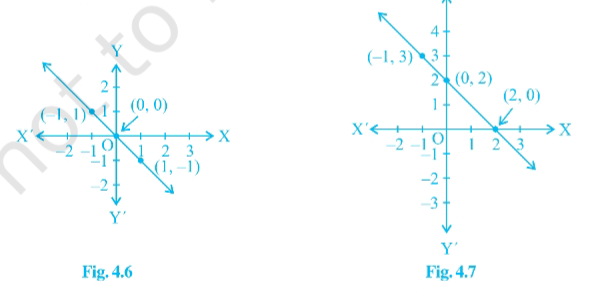
\includegraphics[width=\columnwidth]{chapters/9/figs/4.6-4.7.png}
\caption{Graph}
  \label{fig:4.6-4.7}
\end{figure}
\item If the work done by a body of a constant force is directly proportional 
to the distance travelled by the body,express this in the form of an equation
and draw the graph of the same by taking the varables and draw the graph of 
the same by taking the constant force as $5 units$.Also read from the graph the
work done when the distance travelled by the body is
\begin{enumerate}[label=(\roman*)]
\item $2$Units
\item $0$Unit
\end{enumerate}
\item Yamini and Fatima,two students of class IX of a school,together
 contributed \rupee~100 towards the prime minister's reief fund to help
 the earhquake victims.Write a linear equation which satisfies this data.
 (you may take their contributions  \rupee~x and \rupee~y.Draw the graph 
 of the same.
\item In Countries like USA and Canada temperature is measured in Celsius.
Here is a linear equation that converts Farenheit to celsius:
$F=\frac{9}{5}C+32$
\begin{enumerate}[label=(\roman*)]
\item Draw the graph of the linear equation above using Celsius for $x$
 axis and Farenheit for $y$ axis
\item If the temperature is $30\degree C$,what is the temperature in farenheight?
\item If the temperature is $95\degree F$,what is the temperature in celsius?
\item If the temperature is $0\degree C$.What is the temperature in Farenheit and if the temperature in celsius?
\item Is there a temperature Which is numerically same in both Farenheit and Celsius? If yes find it.
\end{enumerate}
\end{enumerate}

\section{10}
\subsection{Examples:-1-19 (10.3)}
\input{chapters/10/10.3.tex}
\subsection{10.3.1}
\input{chapters/10/10.3.1.tex}
\subsection{10.3.2}
\input{chapters/10/10.3.2.tex}
\subsection{10.3.3}
\begin{enumerate}
\item Solve the following pair of linear equations by the substitution method.
\begin{enumerate}[label=(\roman*)]    
	\item
	\begin{align}
   	 x+y=14 \\x-y=4
	\end{align}
    	\item 
	\begin{align}
	s-t=3
	\end{align}
	\item
	\begin{align}
    	3x-y=3\\ 9x-3y=9
	\end{align}
	\begin{align}   	
 	0.2x+0.3y=1.3\\ 0.4x+0.5y=23
	\end{align}
	\item     
	\begin{align}
	\sqrt{2x}+\sqrt{3y}=0\\ \sqrt{3x}-\sqrt{8y}=0
	\end{align}
	\item
	\begin{align}
    	\frac{3x}{2}-\frac{5y}{2}=-2\\ \frac{x}{3}+\frac{y}{2}=\frac{13}{6}
    	\end{align}
	\end{enumerate}
\item Solve $2x+3y=11$ and $2x+4y=-24$ and hence find the value of $m$ for which $y=mx+3$
\item Form the pair of linear equations for the following problems and find their solutions by the substitution method
    \begin{enumerate}[label=(\Roman*)]
    \item The difference between two numbers is $26$ and one number is three times the other. Find them.
    \item The larger of two supplementary angles exceeds the smaller by $18$ degrees. Find them.
    \item The coach of a cricket team buys $7$ balls and $6$ balls for \rupee~3800. Later, she buys $3$ bats and $5$ balls for \rupee~1750. Find the cost of each bat and each ball.
    \item The taxi charges in a city consist of a fixed charge together with the charges for the distance covered. For a distance of $10$ km, the charge paid is \rupee~105 and for a distance of $15$ km, the charge paid is \rupee~155. What are the fixed charges and the charge per km? How much does a person have to pay for travelling a distance of 25 km ? 
    \item A fraction becomes $\frac{9}{11}$ if $2$ is added to both the numerator and the denominator. If $3$ is added to both the numerator and the denominator, it becomes $\frac{5}{6}$. Find the fraction.
    \item Five years hence, the age of Jacob will be three times that of his son. Five years ago, Jacob's age was seven times that of his son. What are their present ages?
    \end{enumerate}
\end{enumerate}

\subsection{10.3.4}
\input{chapters/10/10.3.4.tex}
\subsection{10.3.5}
\input{chapters/10/10.3.5.tex}
\subsection{10.3.6}
\begin{enumerate}
\item Solve the following pair of equations by reducing them to a pair of linear equations:
\begin{enumerate}[label=(\roman*)]
\item
\begin{align}
\frac{1}{2x}+\frac{1}{3y}=2 \\ \frac{1}{3x}+\frac{1}{2y}=\frac{13}{6}
\end{align}
\item
\begin{align}
\frac{2}{\sqrt{x}}+\frac{3}{\sqrt{y}}=2\\
\frac{4}{\sqrt{x}}-\frac{9}{\sqrt{y}}=-1
\end{align}
\item
\begin{align}
\frac{4}{x}+3y=14\\ \frac{3}{x}-4y=23
\end{align}
\item
\begin{align}
\frac{5}{x-1}+\frac{1}{y-2}=2\\ \frac{6}{x-1}-\frac{3}{y-2}=1
\end{align}
\item
\begin{align}
\frac{7x-2y}{xy}=5\\ \frac{8x+7y}{xy}=15
\end{align}
\item
\begin{align}
6x+3y=6xy\\ 2x+4y=5xy
\end{align}
\item
\begin{align}
\frac{10}{x+y}+\frac{2}{x-y}=4\\ \frac{15}{x+y}-\frac{5}{x-y}=-2
\end{align}
\item
\begin{align}
\frac{1}{3x+y}+\frac{1}{3x-y}=\frac{3}{4}\\ \frac{1}{2(3x+y)}-\frac{1}{2(3x-y)}=\frac{-1}{8}
\end{align}
\end{enumerate}
\item Formulate the following problems as a pair of equations,and hence find their solutions:
\begin{enumerate}[label=(\roman*)]
\item Ritu can row downstream $20km$ in $2$ hours, and upstream $4km$ in $2$ hours. Find her speed of rowing in still water and the speed of the current.
\item $2$ women and $5$ men can together finish an embroidery work in $4$ days, while $3$ women and $6$ men can finish it in $3$ days. Find the time taken by $1$ women along to finish the work, and also that taken by $1$ men alone.
\item Roohi travels $300 km$ to her home partly by train and partly by bus. She takes $4$ hours if she travels $60km$ by train and the remaining by bus. If she travels $100km$ by train and the remaining by bus, she takes $10$ minutes longer. Find the speed of the train and the bus seperately.
\end{enumerate}
\end{enumerate}

\subsection{10.3.7}
\input{chapters/10/10.3.7.tex}
\chapter{Quadratic Equations}
\section{10}
\subsection{Examples:-1-18 (10.4)}                                               
\input{chapters/10/10.4.tex}
\subsection{10.4.1}
\input{chapters/10/10.4.1.tex}
\subsection{10.4.2}
\input{chapters/10/10.4.2.tex}
\subsection{10.4.3}
\input{chapters/10/10.4.3.tex}
\subsection{10.4.4}
\begin{enumerate}
\item Find the nature of the roots of the following quadratic equations. If real roots exist, find them:
\begin{enumerate}[label=(\roman*)]
\item $2x^2-3x+5=0$
\item $3x^2-4 sqrt 3x+4=0$
\item $2x^2-6x+3=0$
\end{enumerate}
\item Find the values of k for each of the following quadratic equations, so that they hav equal roots:
\begin{enumerate}[label=(\roman*)]
\item $2x^2=kx-3=0$
\item $kx(x-2)+6=0$
\end{enumerate}
\item Is it possible to design a rectangular mango grove whose length is twice its breadth, and the area is  $800m^2$? If so, find its length and breadth.
\item Is the following situation possible? If so, determine their present ages.
\\ The sum of the ages of the two friends is 20 years. Four years ago, the product of their ages in years was $48$.
\item Is it possible to design a rectangular park of perimeter 80m and area of $400m^2$. If so, find its length and breadth.
\end{enumerate}



\chapter{Coordinate Geometry}
\section{10}
\subsection{10.7.1}
\input{chapters/10/10.7.1.tex}
\subsection{10.7.2}
\input{chapters/10/10.7.2.tex}
\subsection{10.7.3}
\input{chapters/10/10.7.3.tex}
\subsection{10.7.4}
\input{chapters/10/10.7.4.tex}
\chapter{Straight Lines}
\section{11}
\subsection{11.10.1}
\input{chapters/11/11.10.1.tex}
\subsection{11.10.2}
\input{chapters/11/11.10.2.tex}
\subsection{11.10.3}
\input{chapters/11/11.10.3.tex}
\chapter{Trigonometry}
\section{Ratios}
\input{./chapters/trig/tri_geo_rt}
\section{The Baudhayana Theorem}
\input{./chapters/trig/tri_geo_baudh}
%
\section{Area of a Triangle}
\input{./chapters/trig/tri_geo_sincos}
\section{Angle Bisectors}
\input{./chapters/trig/ang.tex}
\section{Circumradius}
\input{./chapters/trig/tri_geo_cradius}
\section{Tangent}
\input{./chapters/trig/tangent}
\section{Identities}
\input{./chapters/trig/trig_id.tex}
\chapter{Analytic Geometry}
\section{Vectors}
\input{./chapters/coord/vector}
\section{Altitudes of a Triangle:Line Equation}
\input{./chapters/coord/tri_geo_alt}
\section{Circumcircle: Circle Equation}
\input{./chapters/coord/tri_geo_ccentre}
\section{Tangent}
\input{./chapters/coord/circ_geo_prop}
\chapter{Triangle}
\input{./chapters/exercises/tri_geo_exer}
\chapter{Quadrilateral}
\input{./chapters/exercises/quad_geo_exer}
%
\chapter{Circle}
\section{11}
\subsection{11.11.1}
In each of the following exercise \ref{prob:1} to \ref{prob:5}, find the equation of the circle with:
\begin{enumerate}[label=\arabic*.,ref=\thesubsection.\theenumi]
\item centre $(0,2)$ and radius $2$ \label{prob:1}
\item centre $(-2,3)$ and radius $4$
\item centre $\frac({1}{2},\frac{1}{4})$ and radius $\frac {1}{!2}$
\item centre $(1,1)$ and radius $2$
\item centre $(-a,-b)$ and radius $\sqrt{a^2-b^2}$  \label{prob:5}
\end{enumerate}
In each of the following exercise \ref{prob:6} to \ref{prob:9}, find the centre and radius of the circles
\begin{enumerate}[resume]
\item $(x-5)^2+(y-3)^2=36$ \label{prob:6}
\item $x^2+y^2-4x-8y-45=0$
\item $x^2+y^2-8x+10y-12=0$
\item $2x^2+2y^2-x=0$ \label{prob:9}
\end{enumerate}
\begin{enumerate}[resume]
\item Find the equation of the circle passing through the points $(4,1)$ and $(6,5)$ and whose centre is on the line $4x+y=16$.
\item Find the equation of the circle passing through the points $(2,3)$ and $(-1,1)$ and whose centre is on the line $x-3y-11=0$.
\item Find the equation of the circle with radius 5 whose centre lies on x-axis and passes through the point $(2,3)$.
\item Find the equation of the circle passing through $(0,0)$ and making intercepts $a$ and $b$ on the coordinate axes.
\item Find the equation of a circle with centre $(2,2)$ and passes through the point $(4,5)$.
\item Does the point $(-2.5,3.5)$ lie inside, outside or on the circle $x^2+y^2=25$.
\end{enumerate}



\input{./chapters/exercises/circ_geo_exer}
\chapter{Miscellaneous }
\input{./chapters/exercises/geo_misc}
\iffalse
%\include{ch02} 
\backmatter
\appendix
\chapter{Area of a Circle}
\input{./chapters/area/circ_geo_area}
\fi
%
%\chapter{Proofs}
%   \section{}
%\input{apps/defs.tex}

%  \section{}
%\input{apps/parab.tex}
%  \section{}
%\input{apps/nonparab.tex}
%		\section{}
%\input{apps/params.tex}
\latexprintindex

\end{document}

 

\end{enumerate}

\section{Median}
%\renewcommand{\theequation}{\theenumi}
%\begin{enumerate}[label=\arabic*.,ref=\theenumi]
\begin{enumerate}[label=\thesection.\arabic*.,ref=\thesection.\theenumi]
\numberwithin{equation}{enumi}
\item If $\vec{D}$ divides $BC$ in the ratio $k : 1$,
		\begin{align}
			\vec{D}= \frac{k\vec{C}+\vec{B}}{k+1}
		\end{align}
		Find the mid points $\vec{D}, \vec{E}, \vec{F}$ of the sides $BC, CA$ and $AB$ respectively.
		\\
			\iffalse
\let\negmedspace\undefined
\let\negthickspace\undefined
\documentclass[journal,12pt,twocolumn]{IEEEtran}
\usepackage{cite}
\usepackage{amsmath,amssymb,amsfonts,amsthm}
\usepackage{algorithmic}
\usepackage{graphicx}
\usepackage{textcomp}
\usepackage{xcolor}
\usepackage{txfonts}
\usepackage{listings}
\usepackage{enumitem}
\usepackage{mathtools}
\usepackage{gensymb}
\usepackage[breaklinks=true]{hyperref}
\usepackage{tkz-euclide} % loads  TikZ and tkz-base
\usepackage{listings}
\usepackage{gvv}
%
%\usepackage{setspace}
%\usepackage{gensymb}
%\doublespacing
%\singlespacing

%\usepackage{graphicx}
%\usepackage{amssymb}
%\usepackage{relsize}
%\usepackage[cmex10]{amsmath}
%\usepackage{amsthm}
%\interdisplaylinepenalty=2500
%\savesymbol{iint}
%\usepackage{txfonts}
%\restoresymbol{TXF}{iint}
%\usepackage{wasysym}
%\usepackage{amsthm}
%\usepackage{iithtlc}
%\usepackage{mathrsfs}
%\usepackage{txfonts}
%\usepackage{stfloats}
%\usepackage{bm}
%\usepackage{cite}
%\usepackage{cases}
%\usepackage{subfig}
%\usepackage{xtab}
%\usepackage{longtable}
%\usepackage{multirow}
%\usepackage{algorithm}
%\usepackage{algpseudocode}
%\usepackage{enumitem}
%\usepackage{mathtools}
%\usepackage{tikz}
%\usepackage{circuitikz}
%\usepackage{verbatim}
%\usepackage{tfrupee}
%\usepackage{stmaryrd}
%\usetkzobj{all}
%    \usepackage{color}                                            %%
%    \usepackage{array}                                            %%
%    \usepackage{longtable}                                        %%
%    \usepackage{calc}                                             %%
%    \usepackage{multirow}                                         %%
%    \usepackage{hhline}                                           %%
%    \usepackage{ifthen}                                           %%
  %optionally (for landscape tables embedded in another document): %%
%    \usepackage{lscape}     
%\usepackage{multicol}
%\usepackage{chngcntr}
%\usepackage{enumerate}

%\usepackage{wasysym}
%\documentclass[conference]{IEEEtran}
%\IEEEoverridecommandlockouts
% The preceding line is only needed to identify funding in the first footnote. If that is unneeded, please comment it out.

\newtheorem{theorem}{Theorem}[section]
\newtheorem{problem}{Problem}
\newtheorem{proposition}{Proposition}[section]
\newtheorem{lemma}{Lemma}[section]
\newtheorem{corollary}[theorem]{Corollary}
\newtheorem{example}{Example}[section]
\newtheorem{definition}[problem]{Definition}
%\newtheorem{thm}{Theorem}[section] 
%\newtheorem{defn}[thm]{Definition}
%\newtheorem{algorithm}{Algorithm}[section]
%\newtheorem{cor}{Corollary}
\newcommand{\BEQA}{\begin{eqnarray}}
\newcommand{\EEQA}{\end{eqnarray}}
\newcommand{\define}{\stackrel{\triangle}{=}}
\theoremstyle{remark}
\newtheorem{rem}{Remark}

%\bibliographystyle{ieeetr}
\begin{document}
%
\parindent 0px
\bibliographystyle{IEEEtran}


\vspace{3cm}

\title{
%	\logo{
Solution to 1.2.1
%	}
}
\author{Devansh Jain - EE22BTECH11018}	
%\title{
%	\logo{Matrix Analysis through Octave}{\begin{center}\includegraphics[scale=.24]{tlc}\end{center}}{}{HAMDSP}
%}


% paper title
% can use linebreaks \\ within to get better formatting as desired
%\title{Matrix Analysis through Octave}
%
%
% author names and IEEE memberships
% note positions of commas and nonbreaking spaces ( ~ ) LaTeX will not break
% a structure at a ~ so this keeps an author's name from being broken across
% two lines.
% use \thanks{} to gain access to the first footnote area
% a separate \thanks must be used for each paragraph as LaTeX2e's \thanks
% was not built to handle multiple paragraphs
%

%\author{<-this % stops a space
%\thanks{}}
%}
% note the % following the last \IEEEmembership and also \thanks - 
% these prevent an unwanted space from occurring between the last author name
% and the end of the author line. i.e., if you had this:
% 
% \author{....lastname \thanks{...} \thanks{...} }
%                     ^------------^------------^----Do not want these spaces!
%
% a space would be appended to the last name and could cause every name on that
% line to be shifted left slightly. This is one of those "LaTeX things". For
% instance, "\textbf{A} \textbf{B}" will typeset as "A B" not "AB". To get
% "AB" then you have to do: "\textbf{A}\textbf{B}"
% \thanks is no different in this regard, so shield the last } of each \thanks
% that ends a line with a % and do not let a space in before the next \thanks.
% Spaces after \IEEEmembership other than the last one are OK (and needed) as
% you are supposed to have spaces between the names. For what it is worth,
% this is a minor point as most people would not even notice if the said evil
% space somehow managed to creep in.



% The paper headers
%\markboth{Journal of \LaTeX\ Class Files,~Vol.~6, No.~1, January~2007}%
%{Shell \MakeLowercase{\textit{et al.}}: Bare Demo of IEEEtran.cls for Journals}
% The only time the second header will appear is for the odd numbered pages
% after the title page when using the twoside option.
% 
% *** Note that you probably will NOT want to include the author's ***
% *** name in the headers of peer review papers.                   ***
% You can use \ifCLASSOPTIONpeerreview for conditional compilation here if
% you desire.




% If you want to put a publisher's ID mark on the page you can do it like
% this:
%\IEEEpubid{0000--0000/00\$00.00~\copyright~2007 IEEE}
% Remember, if you use this you must call \IEEEpubidadjcol in the second
% column for its text to clear the IEEEpubid mark.



% make the title area
\maketitle

\newpage

%\tableofcontents

\bigskip

\renewcommand{\thefigure}{\theenumi}
\renewcommand{\thetable}{\theenumi}
%\renewcommand{\theequation}{\theenumi}

%\begin{abstract}
%%\boldmath
%In this letter, an algorithm for evaluating the exact analytical bit error rate  (BER)  for the piecewise linear (PL) combiner for  multiple relays is presented. Previous results were available only for upto three relays. The algorithm is unique in the sense that  the actual mathematical expressions, that are prohibitively large, need not be explicitly obtained. The diversity gain due to multiple relays is shown through plots of the analytical BER, well supported by simulations. 
%
%\end{abstract}
% IEEEtran.cls defaults to using nonbold math in the Abstract.
% This preserves the distinction between vectors and scalars. However,
% if the journal you are submitting to favors bold math in the abstract,
% then you can use LaTeX's standard command \boldmath at the very start
% of the abstract to achieve this. Many IEEE journals frown on math
% in the abstract anyway.

% Note that keywords are not normally used for peerreview papers.
%\begin{IEEEkeywords}
%Cooperative diversity, decode and forward, piecewise linear
%\end{IEEEkeywords}



% For peer review papers, you can put extra information on the cover
% page as needed:
% \ifCLASSOPTIONpeerreview
% \begin{center} \bfseries EDICS Category: 3-BBND \end{center}
% \fi
%
% For peerreview papers, this IEEEtran command inserts a page break and
% creates the second title. It will be ignored for other modes.
%\IEEEpeerreviewmaketitle
Question:
If $\vec{D}$ divides $BC$ in the ratio $k : 1$,
\begin{align}
\vec{D}= \frac{k\vec{C}+\vec{B}}{k+1}
\end{align}
Find the mid points $\vec{D}, \vec{E}, \vec{F}$ of the sides $BC, CA$ and $AB$ respectively.
\newline
Given:
\begin{align}
\vec{A} &= \myvec{1\\-1\\}\\
\vec{B} &= \myvec{-4\\6\\}\\
\vec{C} &= \myvec{-3\\-5\\}
\end{align}
\fi
\solution
Since $\vec{D}$ is the midpoint of $BC$,
\begin{align}
k &= 1\\
\implies \vec{D} &= \frac{\vec{C} + \vec{B}}{2}\\
&= \frac{1}{2}\myvec{-7\\1}
\end{align}
Similarly,
\begin{align}
\vec{E} &= \frac{\vec{A} + \vec{C}}{2}\\
&= \myvec{-1\\-3}\\
\vec{F} &= \frac{\vec{A} + \vec{B}}{2}\\
&= \frac{1}{2}\myvec{-3\\5}
\end{align}
\begin{figure}[H]
\centering
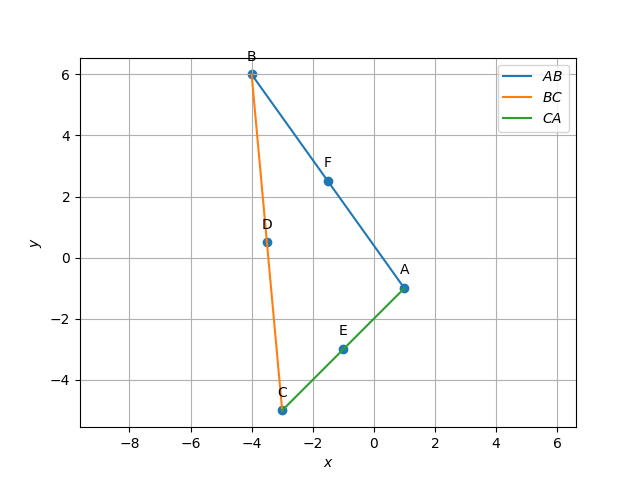
\includegraphics[width=\columnwidth]{solutions/1/2/1/figs/figure.png}
\caption{Triangle ABC with midpoints D,E and F}
\end{figure}
 
	\item Find the equations of $AD, BE$ and $CF$.
	\item Find the intersection $\vec{G}$ of $BE$ and $CF$.
	\item Verify that 
		\begin{align}
			\frac{BG}{GE} = 
			\frac{CG}{GF} =
			\frac{AG}{GD} =2 
		\end{align}
	\item Show that $\vec{A}, \vec{G}$ and $\vec{D}$ are collinear.
	\item Verify that 
		\begin{align}
			\vec{G}=\frac{\vec{A}+\vec{B}+\vec{C}}{3}
		\end{align}
			$\vec{G}$ is known as the {\em centroid} of $\triangle ABC$.
   \\
		%% Run LaTeX on this file several times to get Table of Contents,
%% cross-references, and citations.

\documentclass[11pt]{book}
\usepackage{gvv-book}
\usepackage{gvv}
%\usepackage{Wiley-AuthoringTemplate}
\usepackage[sectionbib,authoryear]{natbib}% for name-date citation comment the below line
%\usepackage[sectionbib,numbers]{natbib}% for numbered citation comment the above line

%%********************************************************************%%
%%       How many levels of section head would you like numbered?     %%
%% 0= no section numbers, 1= section, 2= section, 3= subsection %%
\setcounter{secnumdepth}{3}
%%********************************************************************%%
%%**********************************************************************%%
%%     How many levels of section head would you like to appear in the  %%
%%				Table of Contents?			%%
%% 0= chapter, 1= section, 2= section, 3= subsection titles.	%%
\setcounter{tocdepth}{2}
%%**********************************************************************%%

%\includeonly{ch01}
\makeindex

\begin{document}

\frontmatter
%%%%%%%%%%%%%%%%%%%%%%%%%%%%%%%%%%%%%%%%%%%%%%%%%%%%%%%%%%%%%%%%
%% Title Pages
%% Wiley will provide title and copyright page, but you can make
%% your own titlepages if you'd like anyway
%% Setting up title pages, type in the appropriate names here:

\booktitle{Geometry}

\subtitle{Through Algebra}

\AuAff{G. V. V. Sharma}


%% \\ will start a new line.
%% You may add \affil{} for affiliation, ie,
%\authors{Robert M. Groves\\
%\affil{Universitat de les Illes Balears}
%Floyd J. Fowler, Jr.\\
%\affil{University of New Mexico}
%}

%% Print Half Title and Title Page:
%\halftitlepage
\titlepage

%%%%%%%%%%%%%%%%%%%%%%%%%%%%%%%%%%%%%%%%%%%%%%%%%%%%%%%%%%%%%%%%
%% Copyright Page

\begin{copyrightpage}{2022}
%Title, etc
\end{copyrightpage}

% Note, you must use \ to start indented lines, ie,
% 
% \begin{copyrightpage}{2004}
% Survey Methodology / Robert M. Groves . . . [et al.].
% \       p. cm.---(Wiley series in survey methodology)
% \    ``Wiley-Interscience."
% \    Includes bibliographical references and index.
% \    ISBN 0-471-48348-6 (pbk.)
% \    1. Surveys---Methodology.  2. Social 
% \  sciences---Research---Statistical methods.  I. Groves, Robert M.  II. %
% Series.\\

% HA31.2.S873 2004
% 001.4'33---dc22                                             2004044064
% \end{copyrightpage}

%%%%%%%%%%%%%%%%%%%%%%%%%%%%%%%%%%%%%%%%%%%%%%%%%%%%%%%%%%%%%%%%
%% Only Dedication (optional) 

%\dedication{To my parents}

\tableofcontents

%\listoffigures %optional
%\listoftables  %optional

%% or Contributor Page for edited books
%% before \tableofcontents

%%%%%%%%%%%%%%%%%%%%%%%%%%%%%%%%%%%%%%%%%%%%%%%%%%%%%%%%%%%%%%%%
%  Contributors Page for Edited Book
%%%%%%%%%%%%%%%%%%%%%%%%%%%%%%%%%%%%%%%%%%%%%%%%%%%%%%%%%%%%%%%%

% If your book has chapters written by different authors,
% you'll need a Contributors page.

% Use \begin{contributors}...\end{contributors} and
% then enter each author with the \name{} command, followed
% by the affiliation information.

% \begin{contributors}
% \name{Masayki Abe,} Fujitsu Laboratories Ltd., Fujitsu Limited, Atsugi, Japan
%
% \name{L. A. Akers,} Center for Solid State Electronics Research, Arizona State University, Tempe, Arizona
%
% \name{G. H. Bernstein,} Department of Electrical and Computer Engineering, University of Notre Dame, Notre Dame, South Bend, Indiana; formerly of
% Center for Solid State Electronics Research, Arizona
% State University, Tempe, Arizona 
% \end{contributors}

%%%%%%%%%%%%%%%%%%%%%%%%%%%%%%%%%%%%%%%%%%%%%%%%%%%%%%%%%%%%%%%%
% Optional Foreword:

%\begin{foreword}
%\lipsum[1-2]
%\end{foreword}

%%%%%%%%%%%%%%%%%%%%%%%%%%%%%%%%%%%%%%%%%%%%%%%%%%%%%%%%%%%%%%%%
% Optional Preface:

%\begin{preface}
%\lipsum[1-1]
%\prefaceauthor{}
%\where{place\\
% date}
%\end{preface}

% ie,
% \begin{preface}
% This is an example preface.
% \prefaceauthor{R. K. Watts}
% \where{Durham, North Carolina\\
% September, 2004}

%%%%%%%%%%%%%%%%%%%%%%%%%%%%%%%%%%%%%%%%%%%%%%%%%%%%%%%%%%%%%%%%
% Optional Acknowledgments:

%\acknowledgments
%\lipsum[1-2]
%\authorinitials{I. R. S.}  

%%%%%%%%%%%%%%%%%%%%%%%%%%%%%%%%
%% Glossary Type of Environment:

% \begin{glossary}
% \term{<term>}{<description>}
% \end{glossary}

%%%%%%%%%%%%%%%%%%%%%%%%%%%%%%%%
%\begin{acronyms}
%\acro{ASTA}{Arrivals See Time Averages}
%\acro{BHCA}{Busy Hour Call Attempts}
%\acro{BR}{Bandwidth Reservation}
%\acro{b.u.}{bandwidth unit(s)}
%\acro{CAC}{Call / Connection Admission Control}
%\acro{CBP}{Call Blocking Probability(-ies)}
%\acro{CCS}{Centum Call Seconds}
%\acro{CDTM}{Connection Dependent Threshold Model}
%\acro{CS}{Complete Sharing}
%\acro{DiffServ}{Differentiated Services}
%\acro{EMLM}{Erlang Multirate Loss Model}
%\acro{erl}{The Erlang unit of traffic-load}
%\acro{FIFO}{First in - First out}
%\acro{GB}{Global balance}
%\acro{GoS}{Grade of Service}
%\acro{ICT}{Information and Communication Technology}
%\acro{IntServ}{Integrated Services}
%\acro{IP}{Internet Protocol}
%\acro{ITU-T}{International Telecommunication Unit -- Standardization sector}
%\acro{LB}{Local balance}
%\acro{LHS}{Left hand side}
%\acro{LIFO}{Last in - First out}
%\acro{MMPP}{Markov Modulated Poisson Process}
%\acro{MPLS}{Multiple Protocol Labeling Switching}
%\acro{MRM}{Multi-Retry Model}
%\acro{MTM}{Multi-Threshold Model}
%\acro{PASTA}{Poisson Arrivals See Time Averages}
%\acro{PDF}{Probability Distribution Function}
%\acro{pdf}{probability density function}
%\acro{PFS}{Product Form Solution}
%\acro{QoS}{Quality of Service}
%\acro{r.v.}{random variable(s)}
%\acro{RED}{random early detection}
%\acro{RHS}{Right hand side}
%\acro{RLA}{Reduced Load Approximation}
%\acro{SIRO}{service in random order}
%\acro{SRM}{Single-Retry Model}
%\acro{STM}{Single-Threshold Model}
%\acro{TCP}{Transport Control Protocol}
%\acro{TH}{Threshold(s)}
%\acro{UDP}{User Datagram Protocol}
%\end{acronyms}

\setcounter{page}{1}

\begin{introduction}
This book shows how to solve problems in geometry using trigonometry and coordinate geometry. 

\end{introduction}

\mainmatter

\chapter{Triangle}
Consider a triangle with vertices
		\begin{align}
			\label{eq:tri-pts}
			\vec{A} = \myvec{1 \\ -1},\,
			\vec{B} = \myvec{-4 \\ 6},\,
			\vec{C} = \myvec{-3 \\ -5}
		\end{align}
\section{Vectors}
%\renewcommand{\theequation}{\theenumi}
%\begin{enumerate}[label=\arabic*.,ref=\theenumi]
\begin{enumerate}[label=\thesection.\arabic*.,ref=\thesection.\theenumi]
\numberwithin{equation}{enumi}
\item The direction vector of $AB$ is defined as
		\begin{align}
			\vec{B}-
			\vec{A}
		\end{align}
Find the direction vectors of $AB, BC$ and $CA$.
\\
	\input{solutions/1/1/1/prob_1.tex}
	\item The length of side $BC$ is 
		\begin{align}
			\norm{\vec{B}-\vec{A}} \triangleq \sqrt{\brak{\vec{B}-\vec{A}}^{\top}{\vec{B}-\vec{A}}}
		\end{align}
		where
		\begin{align}
			\vec{A}^{\top}\triangleq\myvec{1 & -1}
		\end{align}
  \\		\input{solutions/1/1/2/main.tex}
\item   Points $\vec{A}, \vec{B}, \vec{C}$ are defined to be collinear if 
		\begin{align}
			\rank{\myvec{1 & 1 & 1 \\ \vec{A}& \vec{B}&\vec{C}}} = 2
		\end{align}
Are the given points in
			\eqref{eq:tri-pts}
collinear?\\
\input{solutions/1/1/3/main.tex}
\item The parameteric form of the equation  of $AB$ is 
		\begin{align}
			\vec{x}=\vec{A}+k\vec{m}
		\end{align}
		where
		\begin{align}
\vec{m}=\vec{B}-\vec{A}
		\end{align}
is the direction vector of $AB$.
Find the parameteric equations of $AB, BC$ and $CA$.
\\
		\input{solutions/1/1/4/main.tex}
\item The normal form of the equation of $AB$  is 
		\begin{align}
			\vec{n}^{\top}\brak{	\vec{x}-\vec{A}} = 0
		\end{align}
		where 
		\begin{align}
			\vec{n}^{\top}\vec{m}&=\vec{n}^{\top}\brak{\vec{B}-\vec{A}} = 0
			\\
			\text{or, } \vec{n}&=\myvec{0 & 1 \\ -1 & 0} \vec{m}
		\end{align}
Find the normal form of the equations of $AB, BC$ and $CA$.
\input{solutions/1/1/5/assign1.tex}
\input{solutions/1/1/5a/assignment1.tex}
\input{solutions/1/1/5c/main.tex}
\item The area of $\triangle ABC$ is defined as
		\begin{align}
			\frac{1}{2}\norm{{\brak{\vec{A}-\vec{B}}\times {\vec{A}-\vec{C}}}}
		\end{align}
		where
		\begin{align}
			\vec{A}\times\vec{B} \triangleq \mydet{1 & -4 \\-1 & 6}
		\end{align}
		Find the area of $\triangle ABC$.\\
  		\input{solutions/1/1/6/main.tex}
	\item Find the angles $A, B, C$ if 
    \label{prop:angle2d}
  \begin{align}
    \label{eq:angle2d}
			\cos A \triangleq 
\frac{\brak{\vec{B}-\vec{A}}^{\top}{\vec{C}-\vec{A}}}{\norm{\vec{B}-\vec{A}}\norm{\vec{C}-\vec{A}}}
  \end{align}\\
  	\input{solutions/1/1/7/main.tex}
\end{enumerate}

\section{Median}
%\renewcommand{\theequation}{\theenumi}
%\begin{enumerate}[label=\arabic*.,ref=\theenumi]
\begin{enumerate}[label=\thesection.\arabic*.,ref=\thesection.\theenumi]
\numberwithin{equation}{enumi}
\item If $\vec{D}$ divides $BC$ in the ratio $k : 1$,
		\begin{align}
			\vec{D}= \frac{k\vec{C}+\vec{B}}{k+1}
		\end{align}
		Find the mid points $\vec{D}, \vec{E}, \vec{F}$ of the sides $BC, CA$ and $AB$ respectively.
		\\
			\input{solutions/1/2/1/main.tex} 
	\item Find the equations of $AD, BE$ and $CF$.
	\item Find the intersection $\vec{G}$ of $BE$ and $CF$.
	\item Verify that 
		\begin{align}
			\frac{BG}{GE} = 
			\frac{CG}{GF} =
			\frac{AG}{GD} =2 
		\end{align}
	\item Show that $\vec{A}, \vec{G}$ and $\vec{D}$ are collinear.
	\item Verify that 
		\begin{align}
			\vec{G}=\frac{\vec{A}+\vec{B}+\vec{C}}{3}
		\end{align}
			$\vec{G}$ is known as the {\em centroid} of $\triangle ABC$.
   \\
		\input{solutions/1/2/6/main.tex}
	\item Verify that 
		\begin{align}
\vec{A}-\vec{F}=\vec{E}-\vec{D}
		\end{align}
		The quadrilateral $AFDE$ is defined to be a parallelogram.
\end{enumerate}

\section{Altitude}
%\renewcommand{\theequation}{\theenumi}
%\begin{enumerate}[label=\arabic*.,ref=\theenumi]
\begin{enumerate}[label=\thesection.\arabic*.,ref=\thesection.\theenumi]
\numberwithin{equation}{enumi}
\item $\vec{D}_1$ is a point on $BC$ such that
		\begin{align}
			AD_1 \perp BC
		\end{align}
		and $AD_1$ is defined to be the altitude. 
		Find the normal vector of $AD_1$.
  \\
		\input{solutions/1/3/1/main.tex}
	\item Find the equation of $AD_1$.

	\item Find the equations of the altitudes $BE_1$ and $CF_1$ to the sides $AC$ and $AB$ respectively. 
	\item Find the intersection $\vec{H}$ of $BE_1$ and $CF_1$.
	\item Verify that 
		\begin{align}
			\brak{\vec{A}-\vec{H}}^{\top}\brak{\vec{B}-\vec{C}} = 0
		\end{align}
  \\
  	\input{solutions/1/3/5/main.tex}
\end{enumerate}

\section{Perpendicular Bisector}
%\renewcommand{\theequation}{\theenumi}
%\begin{enumerate}[label=\arabic*.,ref=\theenumi]
\begin{enumerate}[label=\thesection.\arabic*.,ref=\thesection.\theenumi]
\numberwithin{equation}{enumi}

\item The equation of the perpendicular bisector of $BC$ is
		\begin{align}
			\label{eq:tri-perp-bisect}
			\brak{\vec{x}-\frac{\vec{B}+\vec{C}}{2}}\brak{\vec{B}-\vec{C}} = 0
		\end{align}
		Substitute numerical values and find the equations of the perpendicular bisectors of $AB, BC$ and $CA$.
	\\	\input{solutions/1/4/1/q1.4.1.tex}
	\item Find the intersection $\vec{O}$ of the perpendicular bisectors of $AB$ and $AC$.
 \\
 \input{solutions/1/4/2/main.tex}
	\item Verify that $\vec{O}$ satisfies
			\eqref{eq:tri-perp-bisect}.
$\vec{O}$ is known as the circumcentre.\\
   \input{solutions/1/4/3/main.tex}
		\item Verify that 
		\begin{align}
			OA = OB = OC 
		\end{align}
  \\
  \input{solutions/1/4/4/main.tex}
  \input{solutions/1/4/4(1)/main.tex}
	\item Draw the circle with centre at $\vec{O}$ and radius 
		\begin{align}
			R = OA
		\end{align}
		This is known as the {\em circumradius}. 
  \\  \input{solutions/1/4/5/assignment2.tex}
	\item Verify that 
		\begin{align}
			\angle BOC = 2\angle BAC.
		\end{align}\\
  \input{solutions/1/4/6/Q_1.4.6.tex}
	\item Let 
		\begin{align}
			\vec{P} = \myvec{\cos \theta & -\sin \theta \\ \sin \theta & \cos \theta}
		\end{align}
		Find $\theta$ if 
		\begin{align}
			\vec{C}-\vec{O}=\vec{P}\brak{\vec{A}-\vec{O}}
		\end{align}
\end{enumerate}

\section{Angle Bisector}
%\renewcommand{\theequation}{\theenumi}
%\begin{enumerate}[label=\arabic*.,ref=\theenumi]
\begin{enumerate}[label=\thesection.\arabic*.,ref=\thesection.\theenumi]
\numberwithin{equation}{enumi}
\item Suppose the equations $AB, BC$ and $CA$ are respectively given by 
		\begin{align}
			\label{eq:tri-sides}
			\vec{n}_i^{\top}\vec{x}=c_i \quad i = 1, 2, 3 
		\end{align}
		The equations of the respective angle bisectors are then given by 
		\begin{align}
			\frac{\vec{n}_i^{\top}\vec{x}-c_i}{\norm{\vec{n}_i}}
		=
	\pm	\frac{\vec{n}_j^{\top}\vec{x}-c_j}{\norm{\vec{n}_j}}
\quad i \ne j
		\end{align}
		Substitute numerical values and find the equations of the angle bisectors of $A, B$ and $C$.
	\\
		%\input{solutions/1/5/1/Assignment_1.tex}
  \input{solutions/1/5/1(1)/main.tex}
	\item Find the intersection $\vec{I}$ of the angle bisectors of $B$ and $C$.
 \\
		\input{solutions/1/5/2/main.tex}
	\item Using 
    \eqref{eq:angle2d}
verify that 
		\begin{align}
			\angle BAI = \angle CAI.
		\end{align}
	\item Find the distance from $\vec{I}$ to $BC$.  \\
        \input{solutions/1/5/4/main.tex}
	\item Repeat the above exercise for the sides $AB$ and $AC$.
	\item This distance is known as the {\em inradius} $r$.
	\item Draw a circle with center $\vec{I}$ and radius $r$.  $\vec{I}$ is known as the {\em incentre}.
	\item The equation of the {\em incircle} is given by 
		\begin{align}
			\norm{\vec{x}-\vec{I}}^2 = r^2
		\end{align}
		Find the parameteric equation of $BC$ and use it to verify that $BC$ intersects the incircle at exactly one point $\vec{D}_3$.  $BC$ is defined to be a {\em tangent} to the incircle.  $\vec{D}_3$ is defined to be {\em point of contact}.
	\\
		\input{solutions/1/5/8/main.tex}
  \item Find the other points of contact $\vec{E}_3$ and $\vec{F}_3$.
	\item Verify that 
		\begin{align}
			AE_3 = AF_3=m, BD_3 = BF_3=n, CD_3 = CE_3=p.
		\end{align}
	\item Obtain $m,n,p$ in terms of $a,b,c$, the sides of the triangle using a matrix equation.  Obtain the numerical values.
 \\
 		\input{solutions/1/5/11/main.tex}
\end{enumerate}

%
\chapter{Linear Equations}
\section{9}
\subsection{9.3.3}
\input{chapters/9/9.3.3.tex}
\subsection{9.4.1}
\begin{enumerate}[label=\arabic*.,ref=\theenumi]
\item The cost of a notebook is twice the cost of a pen.Write a linear
equation in two variables to represent this statement.
(Take the Cost of a notebook to be $x$ and that of a pen to be
$y$).
\item Express the following linear equation in the form $ax+by+c=0$
and indicate the values of $a,b$ and $c$ in each case:
%\begin{enumerate}
\begin{enumerate}[label=(\roman*),ref=\theenumi]
\item $2x+3y=9.3\overline{5}$
\item $x-\frac{y}{5}-10=10$
\item $-2x+3y=6$
\item $ x=3y$
\item $2x=-5y$
\item $3x+2=0$
\item $y-2=0$
\item $5=2x$
\end{enumerate}
\end{enumerate}

\subsection{9.4.2}
\input{chapters/9/9.4.2.tex}
\subsection{9.4.3}
\begin{enumerate}[label=\arabic*.,ref=\theenumi]
\item Draw the graph of each of the following linear equations in two variables:
\begin{enumerate}[label=(\roman*),ref=\theenumi]
\item $x+y=4$
\item $x-y=2$
\item $y=3x$
\item $3=2x+y$
\end{enumerate}
\item Give the equations of two lines passing through (2,14).How many more such lines are there and 
why?
\item If the point(3,4) lies on the graph of the equation $3y=ax+7$ find the value of a
\item The taxi fare in the city is as follows:for te first kilometre,the fare is \rupee~8 and for the 
subsquent distance is \rupee~5 per km.Taking the distance Covered as $x$ km and total fare as
\rupee~y.Write a linear equation for this information,and draw its graph.
\item From the choices given below,choose the equation whose graphs are given Fig 4.6 Fig 4.7
\\
For fig-4.6 
\begin{enumerate}[label=(\roman*)]
\item $y=x$
\item $x+y=0$
\item $y=2x$
\item $2+3y=7x$
\end{enumerate} 
For fig-4.7 
\begin{enumerate}[label=(\roman*)]
\item $y=x+2$
\item $y=x-2$
\item $y=-x+2$
\item $x+2y=6$
\end{enumerate}
\begin{figure}[ht]
\centering
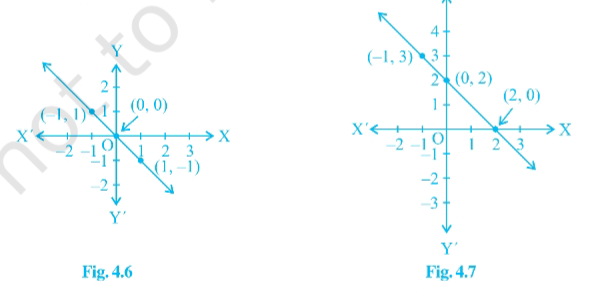
\includegraphics[width=\columnwidth]{chapters/9/figs/4.6-4.7.png}
\caption{Graph}
  \label{fig:4.6-4.7}
\end{figure}
\item If the work done by a body of a constant force is directly proportional 
to the distance travelled by the body,express this in the form of an equation
and draw the graph of the same by taking the varables and draw the graph of 
the same by taking the constant force as $5 units$.Also read from the graph the
work done when the distance travelled by the body is
\begin{enumerate}[label=(\roman*)]
\item $2$Units
\item $0$Unit
\end{enumerate}
\item Yamini and Fatima,two students of class IX of a school,together
 contributed \rupee~100 towards the prime minister's reief fund to help
 the earhquake victims.Write a linear equation which satisfies this data.
 (you may take their contributions  \rupee~x and \rupee~y.Draw the graph 
 of the same.
\item In Countries like USA and Canada temperature is measured in Celsius.
Here is a linear equation that converts Farenheit to celsius:
$F=\frac{9}{5}C+32$
\begin{enumerate}[label=(\roman*)]
\item Draw the graph of the linear equation above using Celsius for $x$
 axis and Farenheit for $y$ axis
\item If the temperature is $30\degree C$,what is the temperature in farenheight?
\item If the temperature is $95\degree F$,what is the temperature in celsius?
\item If the temperature is $0\degree C$.What is the temperature in Farenheit and if the temperature in celsius?
\item Is there a temperature Which is numerically same in both Farenheit and Celsius? If yes find it.
\end{enumerate}
\end{enumerate}

\section{10}
\subsection{Examples:-1-19 (10.3)}
\input{chapters/10/10.3.tex}
\subsection{10.3.1}
\input{chapters/10/10.3.1.tex}
\subsection{10.3.2}
\input{chapters/10/10.3.2.tex}
\subsection{10.3.3}
\begin{enumerate}
\item Solve the following pair of linear equations by the substitution method.
\begin{enumerate}[label=(\roman*)]    
	\item
	\begin{align}
   	 x+y=14 \\x-y=4
	\end{align}
    	\item 
	\begin{align}
	s-t=3
	\end{align}
	\item
	\begin{align}
    	3x-y=3\\ 9x-3y=9
	\end{align}
	\begin{align}   	
 	0.2x+0.3y=1.3\\ 0.4x+0.5y=23
	\end{align}
	\item     
	\begin{align}
	\sqrt{2x}+\sqrt{3y}=0\\ \sqrt{3x}-\sqrt{8y}=0
	\end{align}
	\item
	\begin{align}
    	\frac{3x}{2}-\frac{5y}{2}=-2\\ \frac{x}{3}+\frac{y}{2}=\frac{13}{6}
    	\end{align}
	\end{enumerate}
\item Solve $2x+3y=11$ and $2x+4y=-24$ and hence find the value of $m$ for which $y=mx+3$
\item Form the pair of linear equations for the following problems and find their solutions by the substitution method
    \begin{enumerate}[label=(\Roman*)]
    \item The difference between two numbers is $26$ and one number is three times the other. Find them.
    \item The larger of two supplementary angles exceeds the smaller by $18$ degrees. Find them.
    \item The coach of a cricket team buys $7$ balls and $6$ balls for \rupee~3800. Later, she buys $3$ bats and $5$ balls for \rupee~1750. Find the cost of each bat and each ball.
    \item The taxi charges in a city consist of a fixed charge together with the charges for the distance covered. For a distance of $10$ km, the charge paid is \rupee~105 and for a distance of $15$ km, the charge paid is \rupee~155. What are the fixed charges and the charge per km? How much does a person have to pay for travelling a distance of 25 km ? 
    \item A fraction becomes $\frac{9}{11}$ if $2$ is added to both the numerator and the denominator. If $3$ is added to both the numerator and the denominator, it becomes $\frac{5}{6}$. Find the fraction.
    \item Five years hence, the age of Jacob will be three times that of his son. Five years ago, Jacob's age was seven times that of his son. What are their present ages?
    \end{enumerate}
\end{enumerate}

\subsection{10.3.4}
\input{chapters/10/10.3.4.tex}
\subsection{10.3.5}
\input{chapters/10/10.3.5.tex}
\subsection{10.3.6}
\begin{enumerate}
\item Solve the following pair of equations by reducing them to a pair of linear equations:
\begin{enumerate}[label=(\roman*)]
\item
\begin{align}
\frac{1}{2x}+\frac{1}{3y}=2 \\ \frac{1}{3x}+\frac{1}{2y}=\frac{13}{6}
\end{align}
\item
\begin{align}
\frac{2}{\sqrt{x}}+\frac{3}{\sqrt{y}}=2\\
\frac{4}{\sqrt{x}}-\frac{9}{\sqrt{y}}=-1
\end{align}
\item
\begin{align}
\frac{4}{x}+3y=14\\ \frac{3}{x}-4y=23
\end{align}
\item
\begin{align}
\frac{5}{x-1}+\frac{1}{y-2}=2\\ \frac{6}{x-1}-\frac{3}{y-2}=1
\end{align}
\item
\begin{align}
\frac{7x-2y}{xy}=5\\ \frac{8x+7y}{xy}=15
\end{align}
\item
\begin{align}
6x+3y=6xy\\ 2x+4y=5xy
\end{align}
\item
\begin{align}
\frac{10}{x+y}+\frac{2}{x-y}=4\\ \frac{15}{x+y}-\frac{5}{x-y}=-2
\end{align}
\item
\begin{align}
\frac{1}{3x+y}+\frac{1}{3x-y}=\frac{3}{4}\\ \frac{1}{2(3x+y)}-\frac{1}{2(3x-y)}=\frac{-1}{8}
\end{align}
\end{enumerate}
\item Formulate the following problems as a pair of equations,and hence find their solutions:
\begin{enumerate}[label=(\roman*)]
\item Ritu can row downstream $20km$ in $2$ hours, and upstream $4km$ in $2$ hours. Find her speed of rowing in still water and the speed of the current.
\item $2$ women and $5$ men can together finish an embroidery work in $4$ days, while $3$ women and $6$ men can finish it in $3$ days. Find the time taken by $1$ women along to finish the work, and also that taken by $1$ men alone.
\item Roohi travels $300 km$ to her home partly by train and partly by bus. She takes $4$ hours if she travels $60km$ by train and the remaining by bus. If she travels $100km$ by train and the remaining by bus, she takes $10$ minutes longer. Find the speed of the train and the bus seperately.
\end{enumerate}
\end{enumerate}

\subsection{10.3.7}
\input{chapters/10/10.3.7.tex}
\chapter{Quadratic Equations}
\section{10}
\subsection{Examples:-1-18 (10.4)}                                               
\input{chapters/10/10.4.tex}
\subsection{10.4.1}
\input{chapters/10/10.4.1.tex}
\subsection{10.4.2}
\input{chapters/10/10.4.2.tex}
\subsection{10.4.3}
\input{chapters/10/10.4.3.tex}
\subsection{10.4.4}
\begin{enumerate}
\item Find the nature of the roots of the following quadratic equations. If real roots exist, find them:
\begin{enumerate}[label=(\roman*)]
\item $2x^2-3x+5=0$
\item $3x^2-4 sqrt 3x+4=0$
\item $2x^2-6x+3=0$
\end{enumerate}
\item Find the values of k for each of the following quadratic equations, so that they hav equal roots:
\begin{enumerate}[label=(\roman*)]
\item $2x^2=kx-3=0$
\item $kx(x-2)+6=0$
\end{enumerate}
\item Is it possible to design a rectangular mango grove whose length is twice its breadth, and the area is  $800m^2$? If so, find its length and breadth.
\item Is the following situation possible? If so, determine their present ages.
\\ The sum of the ages of the two friends is 20 years. Four years ago, the product of their ages in years was $48$.
\item Is it possible to design a rectangular park of perimeter 80m and area of $400m^2$. If so, find its length and breadth.
\end{enumerate}



\chapter{Coordinate Geometry}
\section{10}
\subsection{10.7.1}
\input{chapters/10/10.7.1.tex}
\subsection{10.7.2}
\input{chapters/10/10.7.2.tex}
\subsection{10.7.3}
\input{chapters/10/10.7.3.tex}
\subsection{10.7.4}
\input{chapters/10/10.7.4.tex}
\chapter{Straight Lines}
\section{11}
\subsection{11.10.1}
\input{chapters/11/11.10.1.tex}
\subsection{11.10.2}
\input{chapters/11/11.10.2.tex}
\subsection{11.10.3}
\input{chapters/11/11.10.3.tex}
\chapter{Trigonometry}
\section{Ratios}
\input{./chapters/trig/tri_geo_rt}
\section{The Baudhayana Theorem}
\input{./chapters/trig/tri_geo_baudh}
%
\section{Area of a Triangle}
\input{./chapters/trig/tri_geo_sincos}
\section{Angle Bisectors}
\input{./chapters/trig/ang.tex}
\section{Circumradius}
\input{./chapters/trig/tri_geo_cradius}
\section{Tangent}
\input{./chapters/trig/tangent}
\section{Identities}
\input{./chapters/trig/trig_id.tex}
\chapter{Analytic Geometry}
\section{Vectors}
\input{./chapters/coord/vector}
\section{Altitudes of a Triangle:Line Equation}
\input{./chapters/coord/tri_geo_alt}
\section{Circumcircle: Circle Equation}
\input{./chapters/coord/tri_geo_ccentre}
\section{Tangent}
\input{./chapters/coord/circ_geo_prop}
\chapter{Triangle}
\input{./chapters/exercises/tri_geo_exer}
\chapter{Quadrilateral}
\input{./chapters/exercises/quad_geo_exer}
%
\chapter{Circle}
\section{11}
\subsection{11.11.1}
In each of the following exercise \ref{prob:1} to \ref{prob:5}, find the equation of the circle with:
\begin{enumerate}[label=\arabic*.,ref=\thesubsection.\theenumi]
\item centre $(0,2)$ and radius $2$ \label{prob:1}
\item centre $(-2,3)$ and radius $4$
\item centre $\frac({1}{2},\frac{1}{4})$ and radius $\frac {1}{!2}$
\item centre $(1,1)$ and radius $2$
\item centre $(-a,-b)$ and radius $\sqrt{a^2-b^2}$  \label{prob:5}
\end{enumerate}
In each of the following exercise \ref{prob:6} to \ref{prob:9}, find the centre and radius of the circles
\begin{enumerate}[resume]
\item $(x-5)^2+(y-3)^2=36$ \label{prob:6}
\item $x^2+y^2-4x-8y-45=0$
\item $x^2+y^2-8x+10y-12=0$
\item $2x^2+2y^2-x=0$ \label{prob:9}
\end{enumerate}
\begin{enumerate}[resume]
\item Find the equation of the circle passing through the points $(4,1)$ and $(6,5)$ and whose centre is on the line $4x+y=16$.
\item Find the equation of the circle passing through the points $(2,3)$ and $(-1,1)$ and whose centre is on the line $x-3y-11=0$.
\item Find the equation of the circle with radius 5 whose centre lies on x-axis and passes through the point $(2,3)$.
\item Find the equation of the circle passing through $(0,0)$ and making intercepts $a$ and $b$ on the coordinate axes.
\item Find the equation of a circle with centre $(2,2)$ and passes through the point $(4,5)$.
\item Does the point $(-2.5,3.5)$ lie inside, outside or on the circle $x^2+y^2=25$.
\end{enumerate}



\input{./chapters/exercises/circ_geo_exer}
\chapter{Miscellaneous }
\input{./chapters/exercises/geo_misc}
\iffalse
%\include{ch02} 
\backmatter
\appendix
\chapter{Area of a Circle}
\input{./chapters/area/circ_geo_area}
\fi
%
%\chapter{Proofs}
%   \section{}
%\input{apps/defs.tex}

%  \section{}
%\input{apps/parab.tex}
%  \section{}
%\input{apps/nonparab.tex}
%		\section{}
%\input{apps/params.tex}
\latexprintindex

\end{document}

 

	\item Verify that 
		\begin{align}
\vec{A}-\vec{F}=\vec{E}-\vec{D}
		\end{align}
		The quadrilateral $AFDE$ is defined to be a parallelogram.
\end{enumerate}

\section{Altitude}
%\renewcommand{\theequation}{\theenumi}
%\begin{enumerate}[label=\arabic*.,ref=\theenumi]
\begin{enumerate}[label=\thesection.\arabic*.,ref=\thesection.\theenumi]
\numberwithin{equation}{enumi}
\item $\vec{D}_1$ is a point on $BC$ such that
		\begin{align}
			AD_1 \perp BC
		\end{align}
		and $AD_1$ is defined to be the altitude. 
		Find the normal vector of $AD_1$.
  \\
		%% Run LaTeX on this file several times to get Table of Contents,
%% cross-references, and citations.

\documentclass[11pt]{book}
\usepackage{gvv-book}
\usepackage{gvv}
%\usepackage{Wiley-AuthoringTemplate}
\usepackage[sectionbib,authoryear]{natbib}% for name-date citation comment the below line
%\usepackage[sectionbib,numbers]{natbib}% for numbered citation comment the above line

%%********************************************************************%%
%%       How many levels of section head would you like numbered?     %%
%% 0= no section numbers, 1= section, 2= section, 3= subsection %%
\setcounter{secnumdepth}{3}
%%********************************************************************%%
%%**********************************************************************%%
%%     How many levels of section head would you like to appear in the  %%
%%				Table of Contents?			%%
%% 0= chapter, 1= section, 2= section, 3= subsection titles.	%%
\setcounter{tocdepth}{2}
%%**********************************************************************%%

%\includeonly{ch01}
\makeindex

\begin{document}

\frontmatter
%%%%%%%%%%%%%%%%%%%%%%%%%%%%%%%%%%%%%%%%%%%%%%%%%%%%%%%%%%%%%%%%
%% Title Pages
%% Wiley will provide title and copyright page, but you can make
%% your own titlepages if you'd like anyway
%% Setting up title pages, type in the appropriate names here:

\booktitle{Geometry}

\subtitle{Through Algebra}

\AuAff{G. V. V. Sharma}


%% \\ will start a new line.
%% You may add \affil{} for affiliation, ie,
%\authors{Robert M. Groves\\
%\affil{Universitat de les Illes Balears}
%Floyd J. Fowler, Jr.\\
%\affil{University of New Mexico}
%}

%% Print Half Title and Title Page:
%\halftitlepage
\titlepage

%%%%%%%%%%%%%%%%%%%%%%%%%%%%%%%%%%%%%%%%%%%%%%%%%%%%%%%%%%%%%%%%
%% Copyright Page

\begin{copyrightpage}{2022}
%Title, etc
\end{copyrightpage}

% Note, you must use \ to start indented lines, ie,
% 
% \begin{copyrightpage}{2004}
% Survey Methodology / Robert M. Groves . . . [et al.].
% \       p. cm.---(Wiley series in survey methodology)
% \    ``Wiley-Interscience."
% \    Includes bibliographical references and index.
% \    ISBN 0-471-48348-6 (pbk.)
% \    1. Surveys---Methodology.  2. Social 
% \  sciences---Research---Statistical methods.  I. Groves, Robert M.  II. %
% Series.\\

% HA31.2.S873 2004
% 001.4'33---dc22                                             2004044064
% \end{copyrightpage}

%%%%%%%%%%%%%%%%%%%%%%%%%%%%%%%%%%%%%%%%%%%%%%%%%%%%%%%%%%%%%%%%
%% Only Dedication (optional) 

%\dedication{To my parents}

\tableofcontents

%\listoffigures %optional
%\listoftables  %optional

%% or Contributor Page for edited books
%% before \tableofcontents

%%%%%%%%%%%%%%%%%%%%%%%%%%%%%%%%%%%%%%%%%%%%%%%%%%%%%%%%%%%%%%%%
%  Contributors Page for Edited Book
%%%%%%%%%%%%%%%%%%%%%%%%%%%%%%%%%%%%%%%%%%%%%%%%%%%%%%%%%%%%%%%%

% If your book has chapters written by different authors,
% you'll need a Contributors page.

% Use \begin{contributors}...\end{contributors} and
% then enter each author with the \name{} command, followed
% by the affiliation information.

% \begin{contributors}
% \name{Masayki Abe,} Fujitsu Laboratories Ltd., Fujitsu Limited, Atsugi, Japan
%
% \name{L. A. Akers,} Center for Solid State Electronics Research, Arizona State University, Tempe, Arizona
%
% \name{G. H. Bernstein,} Department of Electrical and Computer Engineering, University of Notre Dame, Notre Dame, South Bend, Indiana; formerly of
% Center for Solid State Electronics Research, Arizona
% State University, Tempe, Arizona 
% \end{contributors}

%%%%%%%%%%%%%%%%%%%%%%%%%%%%%%%%%%%%%%%%%%%%%%%%%%%%%%%%%%%%%%%%
% Optional Foreword:

%\begin{foreword}
%\lipsum[1-2]
%\end{foreword}

%%%%%%%%%%%%%%%%%%%%%%%%%%%%%%%%%%%%%%%%%%%%%%%%%%%%%%%%%%%%%%%%
% Optional Preface:

%\begin{preface}
%\lipsum[1-1]
%\prefaceauthor{}
%\where{place\\
% date}
%\end{preface}

% ie,
% \begin{preface}
% This is an example preface.
% \prefaceauthor{R. K. Watts}
% \where{Durham, North Carolina\\
% September, 2004}

%%%%%%%%%%%%%%%%%%%%%%%%%%%%%%%%%%%%%%%%%%%%%%%%%%%%%%%%%%%%%%%%
% Optional Acknowledgments:

%\acknowledgments
%\lipsum[1-2]
%\authorinitials{I. R. S.}  

%%%%%%%%%%%%%%%%%%%%%%%%%%%%%%%%
%% Glossary Type of Environment:

% \begin{glossary}
% \term{<term>}{<description>}
% \end{glossary}

%%%%%%%%%%%%%%%%%%%%%%%%%%%%%%%%
%\begin{acronyms}
%\acro{ASTA}{Arrivals See Time Averages}
%\acro{BHCA}{Busy Hour Call Attempts}
%\acro{BR}{Bandwidth Reservation}
%\acro{b.u.}{bandwidth unit(s)}
%\acro{CAC}{Call / Connection Admission Control}
%\acro{CBP}{Call Blocking Probability(-ies)}
%\acro{CCS}{Centum Call Seconds}
%\acro{CDTM}{Connection Dependent Threshold Model}
%\acro{CS}{Complete Sharing}
%\acro{DiffServ}{Differentiated Services}
%\acro{EMLM}{Erlang Multirate Loss Model}
%\acro{erl}{The Erlang unit of traffic-load}
%\acro{FIFO}{First in - First out}
%\acro{GB}{Global balance}
%\acro{GoS}{Grade of Service}
%\acro{ICT}{Information and Communication Technology}
%\acro{IntServ}{Integrated Services}
%\acro{IP}{Internet Protocol}
%\acro{ITU-T}{International Telecommunication Unit -- Standardization sector}
%\acro{LB}{Local balance}
%\acro{LHS}{Left hand side}
%\acro{LIFO}{Last in - First out}
%\acro{MMPP}{Markov Modulated Poisson Process}
%\acro{MPLS}{Multiple Protocol Labeling Switching}
%\acro{MRM}{Multi-Retry Model}
%\acro{MTM}{Multi-Threshold Model}
%\acro{PASTA}{Poisson Arrivals See Time Averages}
%\acro{PDF}{Probability Distribution Function}
%\acro{pdf}{probability density function}
%\acro{PFS}{Product Form Solution}
%\acro{QoS}{Quality of Service}
%\acro{r.v.}{random variable(s)}
%\acro{RED}{random early detection}
%\acro{RHS}{Right hand side}
%\acro{RLA}{Reduced Load Approximation}
%\acro{SIRO}{service in random order}
%\acro{SRM}{Single-Retry Model}
%\acro{STM}{Single-Threshold Model}
%\acro{TCP}{Transport Control Protocol}
%\acro{TH}{Threshold(s)}
%\acro{UDP}{User Datagram Protocol}
%\end{acronyms}

\setcounter{page}{1}

\begin{introduction}
This book shows how to solve problems in geometry using trigonometry and coordinate geometry. 

\end{introduction}

\mainmatter

\chapter{Triangle}
Consider a triangle with vertices
		\begin{align}
			\label{eq:tri-pts}
			\vec{A} = \myvec{1 \\ -1},\,
			\vec{B} = \myvec{-4 \\ 6},\,
			\vec{C} = \myvec{-3 \\ -5}
		\end{align}
\section{Vectors}
%\renewcommand{\theequation}{\theenumi}
%\begin{enumerate}[label=\arabic*.,ref=\theenumi]
\begin{enumerate}[label=\thesection.\arabic*.,ref=\thesection.\theenumi]
\numberwithin{equation}{enumi}
\item The direction vector of $AB$ is defined as
		\begin{align}
			\vec{B}-
			\vec{A}
		\end{align}
Find the direction vectors of $AB, BC$ and $CA$.
\\
	\input{solutions/1/1/1/prob_1.tex}
	\item The length of side $BC$ is 
		\begin{align}
			\norm{\vec{B}-\vec{A}} \triangleq \sqrt{\brak{\vec{B}-\vec{A}}^{\top}{\vec{B}-\vec{A}}}
		\end{align}
		where
		\begin{align}
			\vec{A}^{\top}\triangleq\myvec{1 & -1}
		\end{align}
  \\		\input{solutions/1/1/2/main.tex}
\item   Points $\vec{A}, \vec{B}, \vec{C}$ are defined to be collinear if 
		\begin{align}
			\rank{\myvec{1 & 1 & 1 \\ \vec{A}& \vec{B}&\vec{C}}} = 2
		\end{align}
Are the given points in
			\eqref{eq:tri-pts}
collinear?\\
\input{solutions/1/1/3/main.tex}
\item The parameteric form of the equation  of $AB$ is 
		\begin{align}
			\vec{x}=\vec{A}+k\vec{m}
		\end{align}
		where
		\begin{align}
\vec{m}=\vec{B}-\vec{A}
		\end{align}
is the direction vector of $AB$.
Find the parameteric equations of $AB, BC$ and $CA$.
\\
		\input{solutions/1/1/4/main.tex}
\item The normal form of the equation of $AB$  is 
		\begin{align}
			\vec{n}^{\top}\brak{	\vec{x}-\vec{A}} = 0
		\end{align}
		where 
		\begin{align}
			\vec{n}^{\top}\vec{m}&=\vec{n}^{\top}\brak{\vec{B}-\vec{A}} = 0
			\\
			\text{or, } \vec{n}&=\myvec{0 & 1 \\ -1 & 0} \vec{m}
		\end{align}
Find the normal form of the equations of $AB, BC$ and $CA$.
\input{solutions/1/1/5/assign1.tex}
\input{solutions/1/1/5a/assignment1.tex}
\input{solutions/1/1/5c/main.tex}
\item The area of $\triangle ABC$ is defined as
		\begin{align}
			\frac{1}{2}\norm{{\brak{\vec{A}-\vec{B}}\times {\vec{A}-\vec{C}}}}
		\end{align}
		where
		\begin{align}
			\vec{A}\times\vec{B} \triangleq \mydet{1 & -4 \\-1 & 6}
		\end{align}
		Find the area of $\triangle ABC$.\\
  		\input{solutions/1/1/6/main.tex}
	\item Find the angles $A, B, C$ if 
    \label{prop:angle2d}
  \begin{align}
    \label{eq:angle2d}
			\cos A \triangleq 
\frac{\brak{\vec{B}-\vec{A}}^{\top}{\vec{C}-\vec{A}}}{\norm{\vec{B}-\vec{A}}\norm{\vec{C}-\vec{A}}}
  \end{align}\\
  	\input{solutions/1/1/7/main.tex}
\end{enumerate}

\section{Median}
%\renewcommand{\theequation}{\theenumi}
%\begin{enumerate}[label=\arabic*.,ref=\theenumi]
\begin{enumerate}[label=\thesection.\arabic*.,ref=\thesection.\theenumi]
\numberwithin{equation}{enumi}
\item If $\vec{D}$ divides $BC$ in the ratio $k : 1$,
		\begin{align}
			\vec{D}= \frac{k\vec{C}+\vec{B}}{k+1}
		\end{align}
		Find the mid points $\vec{D}, \vec{E}, \vec{F}$ of the sides $BC, CA$ and $AB$ respectively.
		\\
			\input{solutions/1/2/1/main.tex} 
	\item Find the equations of $AD, BE$ and $CF$.
	\item Find the intersection $\vec{G}$ of $BE$ and $CF$.
	\item Verify that 
		\begin{align}
			\frac{BG}{GE} = 
			\frac{CG}{GF} =
			\frac{AG}{GD} =2 
		\end{align}
	\item Show that $\vec{A}, \vec{G}$ and $\vec{D}$ are collinear.
	\item Verify that 
		\begin{align}
			\vec{G}=\frac{\vec{A}+\vec{B}+\vec{C}}{3}
		\end{align}
			$\vec{G}$ is known as the {\em centroid} of $\triangle ABC$.
   \\
		\input{solutions/1/2/6/main.tex}
	\item Verify that 
		\begin{align}
\vec{A}-\vec{F}=\vec{E}-\vec{D}
		\end{align}
		The quadrilateral $AFDE$ is defined to be a parallelogram.
\end{enumerate}

\section{Altitude}
%\renewcommand{\theequation}{\theenumi}
%\begin{enumerate}[label=\arabic*.,ref=\theenumi]
\begin{enumerate}[label=\thesection.\arabic*.,ref=\thesection.\theenumi]
\numberwithin{equation}{enumi}
\item $\vec{D}_1$ is a point on $BC$ such that
		\begin{align}
			AD_1 \perp BC
		\end{align}
		and $AD_1$ is defined to be the altitude. 
		Find the normal vector of $AD_1$.
  \\
		\input{solutions/1/3/1/main.tex}
	\item Find the equation of $AD_1$.

	\item Find the equations of the altitudes $BE_1$ and $CF_1$ to the sides $AC$ and $AB$ respectively. 
	\item Find the intersection $\vec{H}$ of $BE_1$ and $CF_1$.
	\item Verify that 
		\begin{align}
			\brak{\vec{A}-\vec{H}}^{\top}\brak{\vec{B}-\vec{C}} = 0
		\end{align}
  \\
  	\input{solutions/1/3/5/main.tex}
\end{enumerate}

\section{Perpendicular Bisector}
%\renewcommand{\theequation}{\theenumi}
%\begin{enumerate}[label=\arabic*.,ref=\theenumi]
\begin{enumerate}[label=\thesection.\arabic*.,ref=\thesection.\theenumi]
\numberwithin{equation}{enumi}

\item The equation of the perpendicular bisector of $BC$ is
		\begin{align}
			\label{eq:tri-perp-bisect}
			\brak{\vec{x}-\frac{\vec{B}+\vec{C}}{2}}\brak{\vec{B}-\vec{C}} = 0
		\end{align}
		Substitute numerical values and find the equations of the perpendicular bisectors of $AB, BC$ and $CA$.
	\\	\input{solutions/1/4/1/q1.4.1.tex}
	\item Find the intersection $\vec{O}$ of the perpendicular bisectors of $AB$ and $AC$.
 \\
 \input{solutions/1/4/2/main.tex}
	\item Verify that $\vec{O}$ satisfies
			\eqref{eq:tri-perp-bisect}.
$\vec{O}$ is known as the circumcentre.\\
   \input{solutions/1/4/3/main.tex}
		\item Verify that 
		\begin{align}
			OA = OB = OC 
		\end{align}
  \\
  \input{solutions/1/4/4/main.tex}
  \input{solutions/1/4/4(1)/main.tex}
	\item Draw the circle with centre at $\vec{O}$ and radius 
		\begin{align}
			R = OA
		\end{align}
		This is known as the {\em circumradius}. 
  \\  \input{solutions/1/4/5/assignment2.tex}
	\item Verify that 
		\begin{align}
			\angle BOC = 2\angle BAC.
		\end{align}\\
  \input{solutions/1/4/6/Q_1.4.6.tex}
	\item Let 
		\begin{align}
			\vec{P} = \myvec{\cos \theta & -\sin \theta \\ \sin \theta & \cos \theta}
		\end{align}
		Find $\theta$ if 
		\begin{align}
			\vec{C}-\vec{O}=\vec{P}\brak{\vec{A}-\vec{O}}
		\end{align}
\end{enumerate}

\section{Angle Bisector}
%\renewcommand{\theequation}{\theenumi}
%\begin{enumerate}[label=\arabic*.,ref=\theenumi]
\begin{enumerate}[label=\thesection.\arabic*.,ref=\thesection.\theenumi]
\numberwithin{equation}{enumi}
\item Suppose the equations $AB, BC$ and $CA$ are respectively given by 
		\begin{align}
			\label{eq:tri-sides}
			\vec{n}_i^{\top}\vec{x}=c_i \quad i = 1, 2, 3 
		\end{align}
		The equations of the respective angle bisectors are then given by 
		\begin{align}
			\frac{\vec{n}_i^{\top}\vec{x}-c_i}{\norm{\vec{n}_i}}
		=
	\pm	\frac{\vec{n}_j^{\top}\vec{x}-c_j}{\norm{\vec{n}_j}}
\quad i \ne j
		\end{align}
		Substitute numerical values and find the equations of the angle bisectors of $A, B$ and $C$.
	\\
		%\input{solutions/1/5/1/Assignment_1.tex}
  \input{solutions/1/5/1(1)/main.tex}
	\item Find the intersection $\vec{I}$ of the angle bisectors of $B$ and $C$.
 \\
		\input{solutions/1/5/2/main.tex}
	\item Using 
    \eqref{eq:angle2d}
verify that 
		\begin{align}
			\angle BAI = \angle CAI.
		\end{align}
	\item Find the distance from $\vec{I}$ to $BC$.  \\
        \input{solutions/1/5/4/main.tex}
	\item Repeat the above exercise for the sides $AB$ and $AC$.
	\item This distance is known as the {\em inradius} $r$.
	\item Draw a circle with center $\vec{I}$ and radius $r$.  $\vec{I}$ is known as the {\em incentre}.
	\item The equation of the {\em incircle} is given by 
		\begin{align}
			\norm{\vec{x}-\vec{I}}^2 = r^2
		\end{align}
		Find the parameteric equation of $BC$ and use it to verify that $BC$ intersects the incircle at exactly one point $\vec{D}_3$.  $BC$ is defined to be a {\em tangent} to the incircle.  $\vec{D}_3$ is defined to be {\em point of contact}.
	\\
		\input{solutions/1/5/8/main.tex}
  \item Find the other points of contact $\vec{E}_3$ and $\vec{F}_3$.
	\item Verify that 
		\begin{align}
			AE_3 = AF_3=m, BD_3 = BF_3=n, CD_3 = CE_3=p.
		\end{align}
	\item Obtain $m,n,p$ in terms of $a,b,c$, the sides of the triangle using a matrix equation.  Obtain the numerical values.
 \\
 		\input{solutions/1/5/11/main.tex}
\end{enumerate}

%
\chapter{Linear Equations}
\section{9}
\subsection{9.3.3}
\input{chapters/9/9.3.3.tex}
\subsection{9.4.1}
\begin{enumerate}[label=\arabic*.,ref=\theenumi]
\item The cost of a notebook is twice the cost of a pen.Write a linear
equation in two variables to represent this statement.
(Take the Cost of a notebook to be $x$ and that of a pen to be
$y$).
\item Express the following linear equation in the form $ax+by+c=0$
and indicate the values of $a,b$ and $c$ in each case:
%\begin{enumerate}
\begin{enumerate}[label=(\roman*),ref=\theenumi]
\item $2x+3y=9.3\overline{5}$
\item $x-\frac{y}{5}-10=10$
\item $-2x+3y=6$
\item $ x=3y$
\item $2x=-5y$
\item $3x+2=0$
\item $y-2=0$
\item $5=2x$
\end{enumerate}
\end{enumerate}

\subsection{9.4.2}
\input{chapters/9/9.4.2.tex}
\subsection{9.4.3}
\begin{enumerate}[label=\arabic*.,ref=\theenumi]
\item Draw the graph of each of the following linear equations in two variables:
\begin{enumerate}[label=(\roman*),ref=\theenumi]
\item $x+y=4$
\item $x-y=2$
\item $y=3x$
\item $3=2x+y$
\end{enumerate}
\item Give the equations of two lines passing through (2,14).How many more such lines are there and 
why?
\item If the point(3,4) lies on the graph of the equation $3y=ax+7$ find the value of a
\item The taxi fare in the city is as follows:for te first kilometre,the fare is \rupee~8 and for the 
subsquent distance is \rupee~5 per km.Taking the distance Covered as $x$ km and total fare as
\rupee~y.Write a linear equation for this information,and draw its graph.
\item From the choices given below,choose the equation whose graphs are given Fig 4.6 Fig 4.7
\\
For fig-4.6 
\begin{enumerate}[label=(\roman*)]
\item $y=x$
\item $x+y=0$
\item $y=2x$
\item $2+3y=7x$
\end{enumerate} 
For fig-4.7 
\begin{enumerate}[label=(\roman*)]
\item $y=x+2$
\item $y=x-2$
\item $y=-x+2$
\item $x+2y=6$
\end{enumerate}
\begin{figure}[ht]
\centering
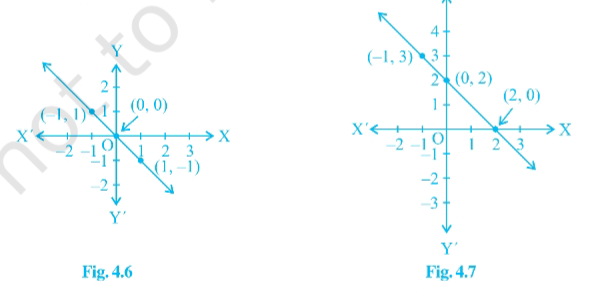
\includegraphics[width=\columnwidth]{chapters/9/figs/4.6-4.7.png}
\caption{Graph}
  \label{fig:4.6-4.7}
\end{figure}
\item If the work done by a body of a constant force is directly proportional 
to the distance travelled by the body,express this in the form of an equation
and draw the graph of the same by taking the varables and draw the graph of 
the same by taking the constant force as $5 units$.Also read from the graph the
work done when the distance travelled by the body is
\begin{enumerate}[label=(\roman*)]
\item $2$Units
\item $0$Unit
\end{enumerate}
\item Yamini and Fatima,two students of class IX of a school,together
 contributed \rupee~100 towards the prime minister's reief fund to help
 the earhquake victims.Write a linear equation which satisfies this data.
 (you may take their contributions  \rupee~x and \rupee~y.Draw the graph 
 of the same.
\item In Countries like USA and Canada temperature is measured in Celsius.
Here is a linear equation that converts Farenheit to celsius:
$F=\frac{9}{5}C+32$
\begin{enumerate}[label=(\roman*)]
\item Draw the graph of the linear equation above using Celsius for $x$
 axis and Farenheit for $y$ axis
\item If the temperature is $30\degree C$,what is the temperature in farenheight?
\item If the temperature is $95\degree F$,what is the temperature in celsius?
\item If the temperature is $0\degree C$.What is the temperature in Farenheit and if the temperature in celsius?
\item Is there a temperature Which is numerically same in both Farenheit and Celsius? If yes find it.
\end{enumerate}
\end{enumerate}

\section{10}
\subsection{Examples:-1-19 (10.3)}
\input{chapters/10/10.3.tex}
\subsection{10.3.1}
\input{chapters/10/10.3.1.tex}
\subsection{10.3.2}
\input{chapters/10/10.3.2.tex}
\subsection{10.3.3}
\begin{enumerate}
\item Solve the following pair of linear equations by the substitution method.
\begin{enumerate}[label=(\roman*)]    
	\item
	\begin{align}
   	 x+y=14 \\x-y=4
	\end{align}
    	\item 
	\begin{align}
	s-t=3
	\end{align}
	\item
	\begin{align}
    	3x-y=3\\ 9x-3y=9
	\end{align}
	\begin{align}   	
 	0.2x+0.3y=1.3\\ 0.4x+0.5y=23
	\end{align}
	\item     
	\begin{align}
	\sqrt{2x}+\sqrt{3y}=0\\ \sqrt{3x}-\sqrt{8y}=0
	\end{align}
	\item
	\begin{align}
    	\frac{3x}{2}-\frac{5y}{2}=-2\\ \frac{x}{3}+\frac{y}{2}=\frac{13}{6}
    	\end{align}
	\end{enumerate}
\item Solve $2x+3y=11$ and $2x+4y=-24$ and hence find the value of $m$ for which $y=mx+3$
\item Form the pair of linear equations for the following problems and find their solutions by the substitution method
    \begin{enumerate}[label=(\Roman*)]
    \item The difference between two numbers is $26$ and one number is three times the other. Find them.
    \item The larger of two supplementary angles exceeds the smaller by $18$ degrees. Find them.
    \item The coach of a cricket team buys $7$ balls and $6$ balls for \rupee~3800. Later, she buys $3$ bats and $5$ balls for \rupee~1750. Find the cost of each bat and each ball.
    \item The taxi charges in a city consist of a fixed charge together with the charges for the distance covered. For a distance of $10$ km, the charge paid is \rupee~105 and for a distance of $15$ km, the charge paid is \rupee~155. What are the fixed charges and the charge per km? How much does a person have to pay for travelling a distance of 25 km ? 
    \item A fraction becomes $\frac{9}{11}$ if $2$ is added to both the numerator and the denominator. If $3$ is added to both the numerator and the denominator, it becomes $\frac{5}{6}$. Find the fraction.
    \item Five years hence, the age of Jacob will be three times that of his son. Five years ago, Jacob's age was seven times that of his son. What are their present ages?
    \end{enumerate}
\end{enumerate}

\subsection{10.3.4}
\input{chapters/10/10.3.4.tex}
\subsection{10.3.5}
\input{chapters/10/10.3.5.tex}
\subsection{10.3.6}
\begin{enumerate}
\item Solve the following pair of equations by reducing them to a pair of linear equations:
\begin{enumerate}[label=(\roman*)]
\item
\begin{align}
\frac{1}{2x}+\frac{1}{3y}=2 \\ \frac{1}{3x}+\frac{1}{2y}=\frac{13}{6}
\end{align}
\item
\begin{align}
\frac{2}{\sqrt{x}}+\frac{3}{\sqrt{y}}=2\\
\frac{4}{\sqrt{x}}-\frac{9}{\sqrt{y}}=-1
\end{align}
\item
\begin{align}
\frac{4}{x}+3y=14\\ \frac{3}{x}-4y=23
\end{align}
\item
\begin{align}
\frac{5}{x-1}+\frac{1}{y-2}=2\\ \frac{6}{x-1}-\frac{3}{y-2}=1
\end{align}
\item
\begin{align}
\frac{7x-2y}{xy}=5\\ \frac{8x+7y}{xy}=15
\end{align}
\item
\begin{align}
6x+3y=6xy\\ 2x+4y=5xy
\end{align}
\item
\begin{align}
\frac{10}{x+y}+\frac{2}{x-y}=4\\ \frac{15}{x+y}-\frac{5}{x-y}=-2
\end{align}
\item
\begin{align}
\frac{1}{3x+y}+\frac{1}{3x-y}=\frac{3}{4}\\ \frac{1}{2(3x+y)}-\frac{1}{2(3x-y)}=\frac{-1}{8}
\end{align}
\end{enumerate}
\item Formulate the following problems as a pair of equations,and hence find their solutions:
\begin{enumerate}[label=(\roman*)]
\item Ritu can row downstream $20km$ in $2$ hours, and upstream $4km$ in $2$ hours. Find her speed of rowing in still water and the speed of the current.
\item $2$ women and $5$ men can together finish an embroidery work in $4$ days, while $3$ women and $6$ men can finish it in $3$ days. Find the time taken by $1$ women along to finish the work, and also that taken by $1$ men alone.
\item Roohi travels $300 km$ to her home partly by train and partly by bus. She takes $4$ hours if she travels $60km$ by train and the remaining by bus. If she travels $100km$ by train and the remaining by bus, she takes $10$ minutes longer. Find the speed of the train and the bus seperately.
\end{enumerate}
\end{enumerate}

\subsection{10.3.7}
\input{chapters/10/10.3.7.tex}
\chapter{Quadratic Equations}
\section{10}
\subsection{Examples:-1-18 (10.4)}                                               
\input{chapters/10/10.4.tex}
\subsection{10.4.1}
\input{chapters/10/10.4.1.tex}
\subsection{10.4.2}
\input{chapters/10/10.4.2.tex}
\subsection{10.4.3}
\input{chapters/10/10.4.3.tex}
\subsection{10.4.4}
\begin{enumerate}
\item Find the nature of the roots of the following quadratic equations. If real roots exist, find them:
\begin{enumerate}[label=(\roman*)]
\item $2x^2-3x+5=0$
\item $3x^2-4 sqrt 3x+4=0$
\item $2x^2-6x+3=0$
\end{enumerate}
\item Find the values of k for each of the following quadratic equations, so that they hav equal roots:
\begin{enumerate}[label=(\roman*)]
\item $2x^2=kx-3=0$
\item $kx(x-2)+6=0$
\end{enumerate}
\item Is it possible to design a rectangular mango grove whose length is twice its breadth, and the area is  $800m^2$? If so, find its length and breadth.
\item Is the following situation possible? If so, determine their present ages.
\\ The sum of the ages of the two friends is 20 years. Four years ago, the product of their ages in years was $48$.
\item Is it possible to design a rectangular park of perimeter 80m and area of $400m^2$. If so, find its length and breadth.
\end{enumerate}



\chapter{Coordinate Geometry}
\section{10}
\subsection{10.7.1}
\input{chapters/10/10.7.1.tex}
\subsection{10.7.2}
\input{chapters/10/10.7.2.tex}
\subsection{10.7.3}
\input{chapters/10/10.7.3.tex}
\subsection{10.7.4}
\input{chapters/10/10.7.4.tex}
\chapter{Straight Lines}
\section{11}
\subsection{11.10.1}
\input{chapters/11/11.10.1.tex}
\subsection{11.10.2}
\input{chapters/11/11.10.2.tex}
\subsection{11.10.3}
\input{chapters/11/11.10.3.tex}
\chapter{Trigonometry}
\section{Ratios}
\input{./chapters/trig/tri_geo_rt}
\section{The Baudhayana Theorem}
\input{./chapters/trig/tri_geo_baudh}
%
\section{Area of a Triangle}
\input{./chapters/trig/tri_geo_sincos}
\section{Angle Bisectors}
\input{./chapters/trig/ang.tex}
\section{Circumradius}
\input{./chapters/trig/tri_geo_cradius}
\section{Tangent}
\input{./chapters/trig/tangent}
\section{Identities}
\input{./chapters/trig/trig_id.tex}
\chapter{Analytic Geometry}
\section{Vectors}
\input{./chapters/coord/vector}
\section{Altitudes of a Triangle:Line Equation}
\input{./chapters/coord/tri_geo_alt}
\section{Circumcircle: Circle Equation}
\input{./chapters/coord/tri_geo_ccentre}
\section{Tangent}
\input{./chapters/coord/circ_geo_prop}
\chapter{Triangle}
\input{./chapters/exercises/tri_geo_exer}
\chapter{Quadrilateral}
\input{./chapters/exercises/quad_geo_exer}
%
\chapter{Circle}
\section{11}
\subsection{11.11.1}
In each of the following exercise \ref{prob:1} to \ref{prob:5}, find the equation of the circle with:
\begin{enumerate}[label=\arabic*.,ref=\thesubsection.\theenumi]
\item centre $(0,2)$ and radius $2$ \label{prob:1}
\item centre $(-2,3)$ and radius $4$
\item centre $\frac({1}{2},\frac{1}{4})$ and radius $\frac {1}{!2}$
\item centre $(1,1)$ and radius $2$
\item centre $(-a,-b)$ and radius $\sqrt{a^2-b^2}$  \label{prob:5}
\end{enumerate}
In each of the following exercise \ref{prob:6} to \ref{prob:9}, find the centre and radius of the circles
\begin{enumerate}[resume]
\item $(x-5)^2+(y-3)^2=36$ \label{prob:6}
\item $x^2+y^2-4x-8y-45=0$
\item $x^2+y^2-8x+10y-12=0$
\item $2x^2+2y^2-x=0$ \label{prob:9}
\end{enumerate}
\begin{enumerate}[resume]
\item Find the equation of the circle passing through the points $(4,1)$ and $(6,5)$ and whose centre is on the line $4x+y=16$.
\item Find the equation of the circle passing through the points $(2,3)$ and $(-1,1)$ and whose centre is on the line $x-3y-11=0$.
\item Find the equation of the circle with radius 5 whose centre lies on x-axis and passes through the point $(2,3)$.
\item Find the equation of the circle passing through $(0,0)$ and making intercepts $a$ and $b$ on the coordinate axes.
\item Find the equation of a circle with centre $(2,2)$ and passes through the point $(4,5)$.
\item Does the point $(-2.5,3.5)$ lie inside, outside or on the circle $x^2+y^2=25$.
\end{enumerate}



\input{./chapters/exercises/circ_geo_exer}
\chapter{Miscellaneous }
\input{./chapters/exercises/geo_misc}
\iffalse
%\include{ch02} 
\backmatter
\appendix
\chapter{Area of a Circle}
\input{./chapters/area/circ_geo_area}
\fi
%
%\chapter{Proofs}
%   \section{}
%\input{apps/defs.tex}

%  \section{}
%\input{apps/parab.tex}
%  \section{}
%\input{apps/nonparab.tex}
%		\section{}
%\input{apps/params.tex}
\latexprintindex

\end{document}

 

	\item Find the equation of $AD_1$.

	\item Find the equations of the altitudes $BE_1$ and $CF_1$ to the sides $AC$ and $AB$ respectively. 
	\item Find the intersection $\vec{H}$ of $BE_1$ and $CF_1$.
	\item Verify that 
		\begin{align}
			\brak{\vec{A}-\vec{H}}^{\top}\brak{\vec{B}-\vec{C}} = 0
		\end{align}
  \\
  	\iffalse
\let\negmedspace\undefined
\let\negthickspace\undefined
\documentclass[journal,12pt,twocolumn]{IEEEtran}
\usepackage{cite}
\usepackage{amsmath,amssymb,amsfonts,amsthm}
\usepackage{algorithmic}
\usepackage{graphicx}
\usepackage{textcomp}
\usepackage{xcolor}
\usepackage{txfonts}
\usepackage{listings}
\usepackage{enumitem}
\usepackage{mathtools}
\usepackage{gensymb}
\usepackage[breaklinks=true]{hyperref}
\usepackage{tkz-euclide} % loads  TikZ and tkz-base
\usepackage{listings}
\usepackage{gvv}
%
%\usepackage{setspace}
%\usepackage{gensymb}
%\doublespacing
%\singlespacing

%\usepackage{graphicx}
%\usepackage{amssymb}
%\usepackage{relsize}
%\usepackage[cmex10]{amsmath}
%\usepackage{amsthm}
%\interdisplaylinepenalty=2500
%\savesymbol{iint}
%\usepackage{txfonts}
%\restoresymbol{TXF}{iint}
%\usepackage{wasysym}
%\usepackage{amsthm}
%\usepackage{iithtlc}
%\usepackage{mathrsfs}
%\usepackage{txfonts}
%\usepackage{stfloats}
%\usepackage{bm}
%\usepackage{cite}
%\usepackage{cases}
%\usepackage{subfig}
%\usepackage{xtab}
%\usepackage{longtable}
%\usepackage{multirow}
%\usepackage{algorithm}
%\usepackage{algpseudocode}
%\usepackage{enumitem}
%\usepackage{mathtools}
%\usepackage{tikz}
%\usepackage{circuitikz}
%\usepackage{verbatim}
%\usepackage{tfrupee}
%\usepackage{stmaryrd}
%\usetkzobj{all}
%    \usepackage{color}                                            %%
%    \usepackage{array}                                            %%
%    \usepackage{longtable}                                        %%
%    \usepackage{calc}                                             %%
%    \usepackage{multirow}                                         %%
%    \usepackage{hhline}                                           %%
%    \usepackage{ifthen}                                           %%
  %optionally (for landscape tables embedded in another document): %%
%    \usepackage{lscape}     
%\usepackage{multicol}
%\usepackage{chngcntr}
%\usepackage{enumerate}

%\usepackage{wasysym}
%\documentclass[conference]{IEEEtran}
%\IEEEoverridecommandlockouts
% The preceding line is only needed to identify funding in the first footnote. If that is unneeded, please comment it out.

\newtheorem{theorem}{Theorem}[section]
\newtheorem{problem}{Problem}
\newtheorem{proposition}{Proposition}[section]
\newtheorem{lemma}{Lemma}[section]
\newtheorem{corollary}[theorem]{Corollary}
\newtheorem{example}{Example}[section]
\newtheorem{definition}[problem]{Definition}
%\newtheorem{thm}{Theorem}[section] 
%\newtheorem{defn}[thm]{Definition}
%\newtheorem{algorithm}{Algorithm}[section]
%\newtheorem{cor}{Corollary}
\newcommand{\BEQA}{\begin{eqnarray}}
\newcommand{\EEQA}{\end{eqnarray}}
\newcommand{\define}{\stackrel{\triangle}{=}}
\theoremstyle{remark}
\newtheorem{rem}{Remark}

%\bibliographystyle{ieeetr}
\begin{document}
%

\bibliographystyle{IEEEtran}


\vspace{3cm}

\title{
%	\logo{
Solution of Question 1.3.5
%	}
}
\author{ Gagan Singla - EE22BTECH11021$^{*}$% <-this % stops a space
	
}	
%\title{
%	\logo{Matrix Analysis through Octave}{\begin{center}\includegraphics[scale=.24]{tlc}\end{center}}{}{HAMDSP}
%}


% paper title
% can use linebreaks \\ within to get better formatting as desired
%\title{Matrix Analysis through Octave}
%
%
% author names and IEEE memberships
% note positions of commas and nonbreaking spaces ( ~ ) LaTeX will not break
% a structure at a ~ so this keeps an author's name from being broken across
% two lines.
% use \thanks{} to gain access to the first footnote area
% a separate \thanks must be used for each paragraph as LaTeX2e's \thanks
% was not built to handle multiple paragraphs
%

%\author{<-this % stops a space
%\thanks{}}
%}
% note the % following the last \IEEEmembership and also \thanks - 
% these prevent an unwanted space from occurring between the last author name
% and the end of the author line. i.e., if you had this:
% 
% \author{....lastname \thanks{...} \thanks{...} }
%                     ^------------^------------^----Do not want these spaces!
%
% a space would be appended to the last name and could cause every name on that
% line to be shifted left slightly. This is one of those "LaTeX things". For
% instance, "\textbf{A} \textbf{B}" will typeset as "A B" not "AB". To get
% "AB" then you have to do: "\textbf{A}\textbf{B}"
% \thanks is no different in this regard, so shield the last } of each \thanks
% that ends a line with a % and do not let a space in before the next \thanks.
% Spaces after \IEEEmembership other than the last one are OK (and needed) as
% you are supposed to have spaces between the names. For what it is worth,
% this is a minor point as most people would not even notice if the said evil
% space somehow managed to creep in.



% The paper headers
%\markboth{Journal of \LaTeX\ Class Files,~Vol.~6, No.~1, January~2007}%
%{Shell \MakeLowercase{\textit{et al.}}: Bare Demo of IEEEtran.cls for Journals}
% The only time the second header will appear is for the odd numbered pages
% after the title page when using the twoside option.
% 
% *** Note that you probably will NOT want to include the author's ***
% *** name in the headers of peer review papers.                   ***
% You can use \ifCLASSOPTIONpeerreview for conditional compilation here if
% you desire.




% If you want to put a publisher's ID mark on the page you can do it like
% this:
%\IEEEpubid{0000--0000/00\$00.00~\copyright~2007 IEEE}
% Remember, if you use this you must call \IEEEpubidadjcol in the second
% column for its text to clear the IEEEpubid mark.



% make the title area
\maketitle

\newpage

%\tableofcontents

\bigskip

\renewcommand{\thefigure}{\theenumi}
\renewcommand{\thetable}{\theenumi}
%\renewcommand{\theequation}{\theenumi}

%\begin{abstract}
%%\boldmath
%In this letter, an algorithm for evaluating the exact analytical bit error rate  (BER)  for the piecewise linear (PL) combiner for  multiple relays is presented. Previous results were available only for upto three relays. The algorithm is unique in the sense that  the actual mathematical expressions, that are prohibitively large, need not be explicitly obtained. The diversity gain due to multiple relays is shown through plots of the analytical BER, well supported by simulations. 
%
%\end{abstract}
% IEEEtran.cls defaults to using nonbold math in the Abstract.
% This preserves the distinction between vectors and scalars. However,
% if the journal you are submitting to favors bold math in the abstract,
% then you can use LaTeX's standard command \boldmath at the very start
% of the abstract to achieve this. Many IEEE journals frown on math
% in the abstract anyway.

% Note that keywords are not normally used for peerreview papers.
%\begin{IEEEkeywords}
%Cooperative diversity, decode and forward, piecewise linear
%\end{IEEEkeywords}



% For peer review papers, you can put extra information on the cover
% page as needed:
% \ifCLASSOPTIONpeerreview
% \begin{center} \bfseries EDICS Category: 3-BBND \end{center}
% \fi
%
% For peerreview papers, this IEEEtran command inserts a page break and
% creates the second title. It will be ignored for other modes.
%\IEEEpeerreviewmaketitle

%\renewcommand{\theequation}{\theenumi}
%\subsection{Problem}

%\section{Chemistry}
%\begin{enumerate}[label=\arabic*.,ref=\thesection.\theenumi]
%\numberwithin{equation}{enumi}

Question: We are given a triangle with vertices $\vec{A}, \vec{B}, \vec{C}$ and the point of intersection of the altitudes drawn from the vertices $\vec{B}$ and $\vec{C}$ is $\vec{H}$. We have to prove that
\begin{align}
\brak{\vec{A} - \vec{H}}^{\top}\brak{\vec{B} - \vec{C}} &= 0
\end{align}
\fi
\solution
\begin{align}
\vec{A} &= \myvec{1\\-1}\\
\vec{B} &= \myvec{-4\\6}\\
\vec{C} &= \myvec{-3\\-5}
\end{align}
The point of intersection of altitutes $BE_1$ and $CF_1$ is:
\begin{align}
\vec{H} &= \myvec{\frac{17}{6}\\\frac{-5}{6}}
\end{align}

\begin{figure}
\centering
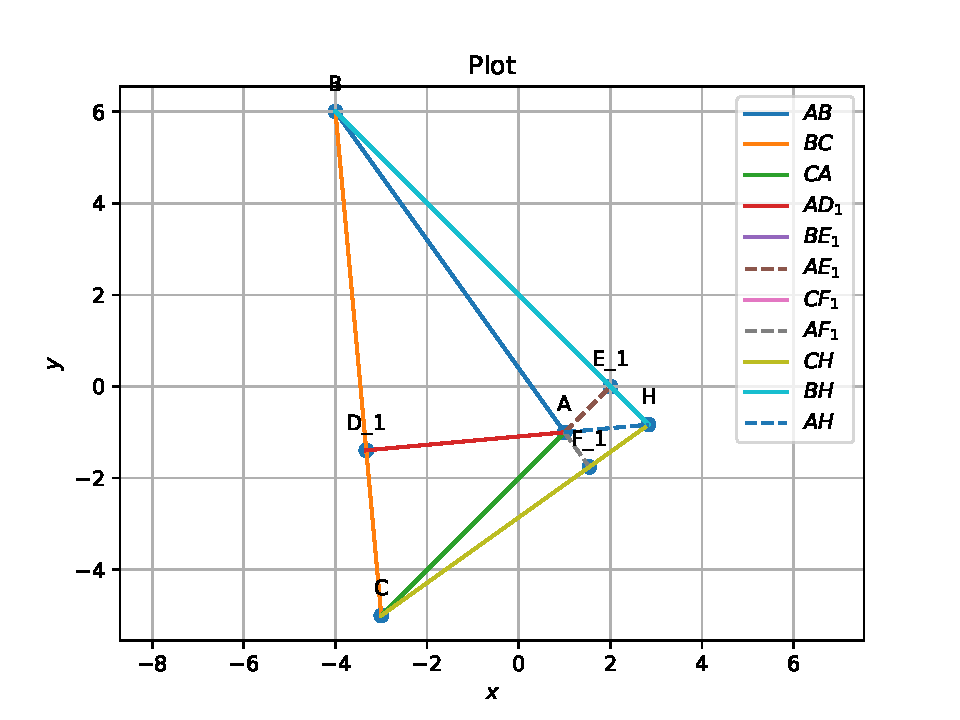
\includegraphics[width=\columnwidth]{solutions/1/3/5/figs/tri_sss.pdf}
\caption{Plot}
\label{fig:Plot}
\end{figure}

Now,
\begin{align}
\vec{A} - \vec{H} &= \myvec{\frac{-11}{6}\\\frac{-1}{6}}\\
\brak{\vec{A} - \vec{H}}^{\top} &= \myvec{\frac{-11}{6}&\frac{-1}{6}}\\
\vec{B} - \vec{C} &= \myvec{-1\\11}\\
\brak{\vec{A} - \vec{H}}^{\top}\brak{\vec{B} - \vec{C}} &= \myvec{\frac{-11}{6}&\frac{-1}{6}}\myvec{-1\\11}\\
&= \frac{11}{6} - \frac{11}{6}\\
&= 0
\end{align}




\end{enumerate}

\section{Perpendicular Bisector}
%\renewcommand{\theequation}{\theenumi}
%\begin{enumerate}[label=\arabic*.,ref=\theenumi]
\begin{enumerate}[label=\thesection.\arabic*.,ref=\thesection.\theenumi]
\numberwithin{equation}{enumi}

\item The equation of the perpendicular bisector of $BC$ is
		\begin{align}
			\label{eq:tri-perp-bisect}
			\brak{\vec{x}-\frac{\vec{B}+\vec{C}}{2}}\brak{\vec{B}-\vec{C}} = 0
		\end{align}
		Substitute numerical values and find the equations of the perpendicular bisectors of $AB, BC$ and $CA$.
	\\	\input{solutions/1/4/1/q1.4.1.tex}
	\item Find the intersection $\vec{O}$ of the perpendicular bisectors of $AB$ and $AC$.
 \\
 %% Run LaTeX on this file several times to get Table of Contents,
%% cross-references, and citations.

\documentclass[11pt]{book}
\usepackage{gvv-book}
\usepackage{gvv}
%\usepackage{Wiley-AuthoringTemplate}
\usepackage[sectionbib,authoryear]{natbib}% for name-date citation comment the below line
%\usepackage[sectionbib,numbers]{natbib}% for numbered citation comment the above line

%%********************************************************************%%
%%       How many levels of section head would you like numbered?     %%
%% 0= no section numbers, 1= section, 2= section, 3= subsection %%
\setcounter{secnumdepth}{3}
%%********************************************************************%%
%%**********************************************************************%%
%%     How many levels of section head would you like to appear in the  %%
%%				Table of Contents?			%%
%% 0= chapter, 1= section, 2= section, 3= subsection titles.	%%
\setcounter{tocdepth}{2}
%%**********************************************************************%%

%\includeonly{ch01}
\makeindex

\begin{document}

\frontmatter
%%%%%%%%%%%%%%%%%%%%%%%%%%%%%%%%%%%%%%%%%%%%%%%%%%%%%%%%%%%%%%%%
%% Title Pages
%% Wiley will provide title and copyright page, but you can make
%% your own titlepages if you'd like anyway
%% Setting up title pages, type in the appropriate names here:

\booktitle{Geometry}

\subtitle{Through Algebra}

\AuAff{G. V. V. Sharma}


%% \\ will start a new line.
%% You may add \affil{} for affiliation, ie,
%\authors{Robert M. Groves\\
%\affil{Universitat de les Illes Balears}
%Floyd J. Fowler, Jr.\\
%\affil{University of New Mexico}
%}

%% Print Half Title and Title Page:
%\halftitlepage
\titlepage

%%%%%%%%%%%%%%%%%%%%%%%%%%%%%%%%%%%%%%%%%%%%%%%%%%%%%%%%%%%%%%%%
%% Copyright Page

\begin{copyrightpage}{2022}
%Title, etc
\end{copyrightpage}

% Note, you must use \ to start indented lines, ie,
% 
% \begin{copyrightpage}{2004}
% Survey Methodology / Robert M. Groves . . . [et al.].
% \       p. cm.---(Wiley series in survey methodology)
% \    ``Wiley-Interscience."
% \    Includes bibliographical references and index.
% \    ISBN 0-471-48348-6 (pbk.)
% \    1. Surveys---Methodology.  2. Social 
% \  sciences---Research---Statistical methods.  I. Groves, Robert M.  II. %
% Series.\\

% HA31.2.S873 2004
% 001.4'33---dc22                                             2004044064
% \end{copyrightpage}

%%%%%%%%%%%%%%%%%%%%%%%%%%%%%%%%%%%%%%%%%%%%%%%%%%%%%%%%%%%%%%%%
%% Only Dedication (optional) 

%\dedication{To my parents}

\tableofcontents

%\listoffigures %optional
%\listoftables  %optional

%% or Contributor Page for edited books
%% before \tableofcontents

%%%%%%%%%%%%%%%%%%%%%%%%%%%%%%%%%%%%%%%%%%%%%%%%%%%%%%%%%%%%%%%%
%  Contributors Page for Edited Book
%%%%%%%%%%%%%%%%%%%%%%%%%%%%%%%%%%%%%%%%%%%%%%%%%%%%%%%%%%%%%%%%

% If your book has chapters written by different authors,
% you'll need a Contributors page.

% Use \begin{contributors}...\end{contributors} and
% then enter each author with the \name{} command, followed
% by the affiliation information.

% \begin{contributors}
% \name{Masayki Abe,} Fujitsu Laboratories Ltd., Fujitsu Limited, Atsugi, Japan
%
% \name{L. A. Akers,} Center for Solid State Electronics Research, Arizona State University, Tempe, Arizona
%
% \name{G. H. Bernstein,} Department of Electrical and Computer Engineering, University of Notre Dame, Notre Dame, South Bend, Indiana; formerly of
% Center for Solid State Electronics Research, Arizona
% State University, Tempe, Arizona 
% \end{contributors}

%%%%%%%%%%%%%%%%%%%%%%%%%%%%%%%%%%%%%%%%%%%%%%%%%%%%%%%%%%%%%%%%
% Optional Foreword:

%\begin{foreword}
%\lipsum[1-2]
%\end{foreword}

%%%%%%%%%%%%%%%%%%%%%%%%%%%%%%%%%%%%%%%%%%%%%%%%%%%%%%%%%%%%%%%%
% Optional Preface:

%\begin{preface}
%\lipsum[1-1]
%\prefaceauthor{}
%\where{place\\
% date}
%\end{preface}

% ie,
% \begin{preface}
% This is an example preface.
% \prefaceauthor{R. K. Watts}
% \where{Durham, North Carolina\\
% September, 2004}

%%%%%%%%%%%%%%%%%%%%%%%%%%%%%%%%%%%%%%%%%%%%%%%%%%%%%%%%%%%%%%%%
% Optional Acknowledgments:

%\acknowledgments
%\lipsum[1-2]
%\authorinitials{I. R. S.}  

%%%%%%%%%%%%%%%%%%%%%%%%%%%%%%%%
%% Glossary Type of Environment:

% \begin{glossary}
% \term{<term>}{<description>}
% \end{glossary}

%%%%%%%%%%%%%%%%%%%%%%%%%%%%%%%%
%\begin{acronyms}
%\acro{ASTA}{Arrivals See Time Averages}
%\acro{BHCA}{Busy Hour Call Attempts}
%\acro{BR}{Bandwidth Reservation}
%\acro{b.u.}{bandwidth unit(s)}
%\acro{CAC}{Call / Connection Admission Control}
%\acro{CBP}{Call Blocking Probability(-ies)}
%\acro{CCS}{Centum Call Seconds}
%\acro{CDTM}{Connection Dependent Threshold Model}
%\acro{CS}{Complete Sharing}
%\acro{DiffServ}{Differentiated Services}
%\acro{EMLM}{Erlang Multirate Loss Model}
%\acro{erl}{The Erlang unit of traffic-load}
%\acro{FIFO}{First in - First out}
%\acro{GB}{Global balance}
%\acro{GoS}{Grade of Service}
%\acro{ICT}{Information and Communication Technology}
%\acro{IntServ}{Integrated Services}
%\acro{IP}{Internet Protocol}
%\acro{ITU-T}{International Telecommunication Unit -- Standardization sector}
%\acro{LB}{Local balance}
%\acro{LHS}{Left hand side}
%\acro{LIFO}{Last in - First out}
%\acro{MMPP}{Markov Modulated Poisson Process}
%\acro{MPLS}{Multiple Protocol Labeling Switching}
%\acro{MRM}{Multi-Retry Model}
%\acro{MTM}{Multi-Threshold Model}
%\acro{PASTA}{Poisson Arrivals See Time Averages}
%\acro{PDF}{Probability Distribution Function}
%\acro{pdf}{probability density function}
%\acro{PFS}{Product Form Solution}
%\acro{QoS}{Quality of Service}
%\acro{r.v.}{random variable(s)}
%\acro{RED}{random early detection}
%\acro{RHS}{Right hand side}
%\acro{RLA}{Reduced Load Approximation}
%\acro{SIRO}{service in random order}
%\acro{SRM}{Single-Retry Model}
%\acro{STM}{Single-Threshold Model}
%\acro{TCP}{Transport Control Protocol}
%\acro{TH}{Threshold(s)}
%\acro{UDP}{User Datagram Protocol}
%\end{acronyms}

\setcounter{page}{1}

\begin{introduction}
This book shows how to solve problems in geometry using trigonometry and coordinate geometry. 

\end{introduction}

\mainmatter

\chapter{Triangle}
Consider a triangle with vertices
		\begin{align}
			\label{eq:tri-pts}
			\vec{A} = \myvec{1 \\ -1},\,
			\vec{B} = \myvec{-4 \\ 6},\,
			\vec{C} = \myvec{-3 \\ -5}
		\end{align}
\section{Vectors}
%\renewcommand{\theequation}{\theenumi}
%\begin{enumerate}[label=\arabic*.,ref=\theenumi]
\begin{enumerate}[label=\thesection.\arabic*.,ref=\thesection.\theenumi]
\numberwithin{equation}{enumi}
\item The direction vector of $AB$ is defined as
		\begin{align}
			\vec{B}-
			\vec{A}
		\end{align}
Find the direction vectors of $AB, BC$ and $CA$.
\\
	\input{solutions/1/1/1/prob_1.tex}
	\item The length of side $BC$ is 
		\begin{align}
			\norm{\vec{B}-\vec{A}} \triangleq \sqrt{\brak{\vec{B}-\vec{A}}^{\top}{\vec{B}-\vec{A}}}
		\end{align}
		where
		\begin{align}
			\vec{A}^{\top}\triangleq\myvec{1 & -1}
		\end{align}
  \\		\input{solutions/1/1/2/main.tex}
\item   Points $\vec{A}, \vec{B}, \vec{C}$ are defined to be collinear if 
		\begin{align}
			\rank{\myvec{1 & 1 & 1 \\ \vec{A}& \vec{B}&\vec{C}}} = 2
		\end{align}
Are the given points in
			\eqref{eq:tri-pts}
collinear?\\
\input{solutions/1/1/3/main.tex}
\item The parameteric form of the equation  of $AB$ is 
		\begin{align}
			\vec{x}=\vec{A}+k\vec{m}
		\end{align}
		where
		\begin{align}
\vec{m}=\vec{B}-\vec{A}
		\end{align}
is the direction vector of $AB$.
Find the parameteric equations of $AB, BC$ and $CA$.
\\
		\input{solutions/1/1/4/main.tex}
\item The normal form of the equation of $AB$  is 
		\begin{align}
			\vec{n}^{\top}\brak{	\vec{x}-\vec{A}} = 0
		\end{align}
		where 
		\begin{align}
			\vec{n}^{\top}\vec{m}&=\vec{n}^{\top}\brak{\vec{B}-\vec{A}} = 0
			\\
			\text{or, } \vec{n}&=\myvec{0 & 1 \\ -1 & 0} \vec{m}
		\end{align}
Find the normal form of the equations of $AB, BC$ and $CA$.
\input{solutions/1/1/5/assign1.tex}
\input{solutions/1/1/5a/assignment1.tex}
\input{solutions/1/1/5c/main.tex}
\item The area of $\triangle ABC$ is defined as
		\begin{align}
			\frac{1}{2}\norm{{\brak{\vec{A}-\vec{B}}\times {\vec{A}-\vec{C}}}}
		\end{align}
		where
		\begin{align}
			\vec{A}\times\vec{B} \triangleq \mydet{1 & -4 \\-1 & 6}
		\end{align}
		Find the area of $\triangle ABC$.\\
  		\input{solutions/1/1/6/main.tex}
	\item Find the angles $A, B, C$ if 
    \label{prop:angle2d}
  \begin{align}
    \label{eq:angle2d}
			\cos A \triangleq 
\frac{\brak{\vec{B}-\vec{A}}^{\top}{\vec{C}-\vec{A}}}{\norm{\vec{B}-\vec{A}}\norm{\vec{C}-\vec{A}}}
  \end{align}\\
  	\input{solutions/1/1/7/main.tex}
\end{enumerate}

\section{Median}
%\renewcommand{\theequation}{\theenumi}
%\begin{enumerate}[label=\arabic*.,ref=\theenumi]
\begin{enumerate}[label=\thesection.\arabic*.,ref=\thesection.\theenumi]
\numberwithin{equation}{enumi}
\item If $\vec{D}$ divides $BC$ in the ratio $k : 1$,
		\begin{align}
			\vec{D}= \frac{k\vec{C}+\vec{B}}{k+1}
		\end{align}
		Find the mid points $\vec{D}, \vec{E}, \vec{F}$ of the sides $BC, CA$ and $AB$ respectively.
		\\
			\input{solutions/1/2/1/main.tex} 
	\item Find the equations of $AD, BE$ and $CF$.
	\item Find the intersection $\vec{G}$ of $BE$ and $CF$.
	\item Verify that 
		\begin{align}
			\frac{BG}{GE} = 
			\frac{CG}{GF} =
			\frac{AG}{GD} =2 
		\end{align}
	\item Show that $\vec{A}, \vec{G}$ and $\vec{D}$ are collinear.
	\item Verify that 
		\begin{align}
			\vec{G}=\frac{\vec{A}+\vec{B}+\vec{C}}{3}
		\end{align}
			$\vec{G}$ is known as the {\em centroid} of $\triangle ABC$.
   \\
		\input{solutions/1/2/6/main.tex}
	\item Verify that 
		\begin{align}
\vec{A}-\vec{F}=\vec{E}-\vec{D}
		\end{align}
		The quadrilateral $AFDE$ is defined to be a parallelogram.
\end{enumerate}

\section{Altitude}
%\renewcommand{\theequation}{\theenumi}
%\begin{enumerate}[label=\arabic*.,ref=\theenumi]
\begin{enumerate}[label=\thesection.\arabic*.,ref=\thesection.\theenumi]
\numberwithin{equation}{enumi}
\item $\vec{D}_1$ is a point on $BC$ such that
		\begin{align}
			AD_1 \perp BC
		\end{align}
		and $AD_1$ is defined to be the altitude. 
		Find the normal vector of $AD_1$.
  \\
		\input{solutions/1/3/1/main.tex}
	\item Find the equation of $AD_1$.

	\item Find the equations of the altitudes $BE_1$ and $CF_1$ to the sides $AC$ and $AB$ respectively. 
	\item Find the intersection $\vec{H}$ of $BE_1$ and $CF_1$.
	\item Verify that 
		\begin{align}
			\brak{\vec{A}-\vec{H}}^{\top}\brak{\vec{B}-\vec{C}} = 0
		\end{align}
  \\
  	\input{solutions/1/3/5/main.tex}
\end{enumerate}

\section{Perpendicular Bisector}
%\renewcommand{\theequation}{\theenumi}
%\begin{enumerate}[label=\arabic*.,ref=\theenumi]
\begin{enumerate}[label=\thesection.\arabic*.,ref=\thesection.\theenumi]
\numberwithin{equation}{enumi}

\item The equation of the perpendicular bisector of $BC$ is
		\begin{align}
			\label{eq:tri-perp-bisect}
			\brak{\vec{x}-\frac{\vec{B}+\vec{C}}{2}}\brak{\vec{B}-\vec{C}} = 0
		\end{align}
		Substitute numerical values and find the equations of the perpendicular bisectors of $AB, BC$ and $CA$.
	\\	\input{solutions/1/4/1/q1.4.1.tex}
	\item Find the intersection $\vec{O}$ of the perpendicular bisectors of $AB$ and $AC$.
 \\
 \input{solutions/1/4/2/main.tex}
	\item Verify that $\vec{O}$ satisfies
			\eqref{eq:tri-perp-bisect}.
$\vec{O}$ is known as the circumcentre.\\
   \input{solutions/1/4/3/main.tex}
		\item Verify that 
		\begin{align}
			OA = OB = OC 
		\end{align}
  \\
  \input{solutions/1/4/4/main.tex}
  \input{solutions/1/4/4(1)/main.tex}
	\item Draw the circle with centre at $\vec{O}$ and radius 
		\begin{align}
			R = OA
		\end{align}
		This is known as the {\em circumradius}. 
  \\  \input{solutions/1/4/5/assignment2.tex}
	\item Verify that 
		\begin{align}
			\angle BOC = 2\angle BAC.
		\end{align}\\
  \input{solutions/1/4/6/Q_1.4.6.tex}
	\item Let 
		\begin{align}
			\vec{P} = \myvec{\cos \theta & -\sin \theta \\ \sin \theta & \cos \theta}
		\end{align}
		Find $\theta$ if 
		\begin{align}
			\vec{C}-\vec{O}=\vec{P}\brak{\vec{A}-\vec{O}}
		\end{align}
\end{enumerate}

\section{Angle Bisector}
%\renewcommand{\theequation}{\theenumi}
%\begin{enumerate}[label=\arabic*.,ref=\theenumi]
\begin{enumerate}[label=\thesection.\arabic*.,ref=\thesection.\theenumi]
\numberwithin{equation}{enumi}
\item Suppose the equations $AB, BC$ and $CA$ are respectively given by 
		\begin{align}
			\label{eq:tri-sides}
			\vec{n}_i^{\top}\vec{x}=c_i \quad i = 1, 2, 3 
		\end{align}
		The equations of the respective angle bisectors are then given by 
		\begin{align}
			\frac{\vec{n}_i^{\top}\vec{x}-c_i}{\norm{\vec{n}_i}}
		=
	\pm	\frac{\vec{n}_j^{\top}\vec{x}-c_j}{\norm{\vec{n}_j}}
\quad i \ne j
		\end{align}
		Substitute numerical values and find the equations of the angle bisectors of $A, B$ and $C$.
	\\
		%\input{solutions/1/5/1/Assignment_1.tex}
  \input{solutions/1/5/1(1)/main.tex}
	\item Find the intersection $\vec{I}$ of the angle bisectors of $B$ and $C$.
 \\
		\input{solutions/1/5/2/main.tex}
	\item Using 
    \eqref{eq:angle2d}
verify that 
		\begin{align}
			\angle BAI = \angle CAI.
		\end{align}
	\item Find the distance from $\vec{I}$ to $BC$.  \\
        \input{solutions/1/5/4/main.tex}
	\item Repeat the above exercise for the sides $AB$ and $AC$.
	\item This distance is known as the {\em inradius} $r$.
	\item Draw a circle with center $\vec{I}$ and radius $r$.  $\vec{I}$ is known as the {\em incentre}.
	\item The equation of the {\em incircle} is given by 
		\begin{align}
			\norm{\vec{x}-\vec{I}}^2 = r^2
		\end{align}
		Find the parameteric equation of $BC$ and use it to verify that $BC$ intersects the incircle at exactly one point $\vec{D}_3$.  $BC$ is defined to be a {\em tangent} to the incircle.  $\vec{D}_3$ is defined to be {\em point of contact}.
	\\
		\input{solutions/1/5/8/main.tex}
  \item Find the other points of contact $\vec{E}_3$ and $\vec{F}_3$.
	\item Verify that 
		\begin{align}
			AE_3 = AF_3=m, BD_3 = BF_3=n, CD_3 = CE_3=p.
		\end{align}
	\item Obtain $m,n,p$ in terms of $a,b,c$, the sides of the triangle using a matrix equation.  Obtain the numerical values.
 \\
 		\input{solutions/1/5/11/main.tex}
\end{enumerate}

%
\chapter{Linear Equations}
\section{9}
\subsection{9.3.3}
\input{chapters/9/9.3.3.tex}
\subsection{9.4.1}
\begin{enumerate}[label=\arabic*.,ref=\theenumi]
\item The cost of a notebook is twice the cost of a pen.Write a linear
equation in two variables to represent this statement.
(Take the Cost of a notebook to be $x$ and that of a pen to be
$y$).
\item Express the following linear equation in the form $ax+by+c=0$
and indicate the values of $a,b$ and $c$ in each case:
%\begin{enumerate}
\begin{enumerate}[label=(\roman*),ref=\theenumi]
\item $2x+3y=9.3\overline{5}$
\item $x-\frac{y}{5}-10=10$
\item $-2x+3y=6$
\item $ x=3y$
\item $2x=-5y$
\item $3x+2=0$
\item $y-2=0$
\item $5=2x$
\end{enumerate}
\end{enumerate}

\subsection{9.4.2}
\input{chapters/9/9.4.2.tex}
\subsection{9.4.3}
\begin{enumerate}[label=\arabic*.,ref=\theenumi]
\item Draw the graph of each of the following linear equations in two variables:
\begin{enumerate}[label=(\roman*),ref=\theenumi]
\item $x+y=4$
\item $x-y=2$
\item $y=3x$
\item $3=2x+y$
\end{enumerate}
\item Give the equations of two lines passing through (2,14).How many more such lines are there and 
why?
\item If the point(3,4) lies on the graph of the equation $3y=ax+7$ find the value of a
\item The taxi fare in the city is as follows:for te first kilometre,the fare is \rupee~8 and for the 
subsquent distance is \rupee~5 per km.Taking the distance Covered as $x$ km and total fare as
\rupee~y.Write a linear equation for this information,and draw its graph.
\item From the choices given below,choose the equation whose graphs are given Fig 4.6 Fig 4.7
\\
For fig-4.6 
\begin{enumerate}[label=(\roman*)]
\item $y=x$
\item $x+y=0$
\item $y=2x$
\item $2+3y=7x$
\end{enumerate} 
For fig-4.7 
\begin{enumerate}[label=(\roman*)]
\item $y=x+2$
\item $y=x-2$
\item $y=-x+2$
\item $x+2y=6$
\end{enumerate}
\begin{figure}[ht]
\centering
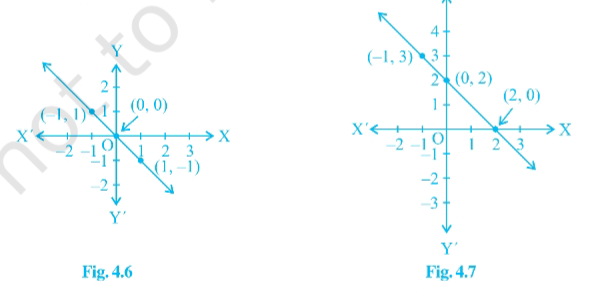
\includegraphics[width=\columnwidth]{chapters/9/figs/4.6-4.7.png}
\caption{Graph}
  \label{fig:4.6-4.7}
\end{figure}
\item If the work done by a body of a constant force is directly proportional 
to the distance travelled by the body,express this in the form of an equation
and draw the graph of the same by taking the varables and draw the graph of 
the same by taking the constant force as $5 units$.Also read from the graph the
work done when the distance travelled by the body is
\begin{enumerate}[label=(\roman*)]
\item $2$Units
\item $0$Unit
\end{enumerate}
\item Yamini and Fatima,two students of class IX of a school,together
 contributed \rupee~100 towards the prime minister's reief fund to help
 the earhquake victims.Write a linear equation which satisfies this data.
 (you may take their contributions  \rupee~x and \rupee~y.Draw the graph 
 of the same.
\item In Countries like USA and Canada temperature is measured in Celsius.
Here is a linear equation that converts Farenheit to celsius:
$F=\frac{9}{5}C+32$
\begin{enumerate}[label=(\roman*)]
\item Draw the graph of the linear equation above using Celsius for $x$
 axis and Farenheit for $y$ axis
\item If the temperature is $30\degree C$,what is the temperature in farenheight?
\item If the temperature is $95\degree F$,what is the temperature in celsius?
\item If the temperature is $0\degree C$.What is the temperature in Farenheit and if the temperature in celsius?
\item Is there a temperature Which is numerically same in both Farenheit and Celsius? If yes find it.
\end{enumerate}
\end{enumerate}

\section{10}
\subsection{Examples:-1-19 (10.3)}
\input{chapters/10/10.3.tex}
\subsection{10.3.1}
\input{chapters/10/10.3.1.tex}
\subsection{10.3.2}
\input{chapters/10/10.3.2.tex}
\subsection{10.3.3}
\begin{enumerate}
\item Solve the following pair of linear equations by the substitution method.
\begin{enumerate}[label=(\roman*)]    
	\item
	\begin{align}
   	 x+y=14 \\x-y=4
	\end{align}
    	\item 
	\begin{align}
	s-t=3
	\end{align}
	\item
	\begin{align}
    	3x-y=3\\ 9x-3y=9
	\end{align}
	\begin{align}   	
 	0.2x+0.3y=1.3\\ 0.4x+0.5y=23
	\end{align}
	\item     
	\begin{align}
	\sqrt{2x}+\sqrt{3y}=0\\ \sqrt{3x}-\sqrt{8y}=0
	\end{align}
	\item
	\begin{align}
    	\frac{3x}{2}-\frac{5y}{2}=-2\\ \frac{x}{3}+\frac{y}{2}=\frac{13}{6}
    	\end{align}
	\end{enumerate}
\item Solve $2x+3y=11$ and $2x+4y=-24$ and hence find the value of $m$ for which $y=mx+3$
\item Form the pair of linear equations for the following problems and find their solutions by the substitution method
    \begin{enumerate}[label=(\Roman*)]
    \item The difference between two numbers is $26$ and one number is three times the other. Find them.
    \item The larger of two supplementary angles exceeds the smaller by $18$ degrees. Find them.
    \item The coach of a cricket team buys $7$ balls and $6$ balls for \rupee~3800. Later, she buys $3$ bats and $5$ balls for \rupee~1750. Find the cost of each bat and each ball.
    \item The taxi charges in a city consist of a fixed charge together with the charges for the distance covered. For a distance of $10$ km, the charge paid is \rupee~105 and for a distance of $15$ km, the charge paid is \rupee~155. What are the fixed charges and the charge per km? How much does a person have to pay for travelling a distance of 25 km ? 
    \item A fraction becomes $\frac{9}{11}$ if $2$ is added to both the numerator and the denominator. If $3$ is added to both the numerator and the denominator, it becomes $\frac{5}{6}$. Find the fraction.
    \item Five years hence, the age of Jacob will be three times that of his son. Five years ago, Jacob's age was seven times that of his son. What are their present ages?
    \end{enumerate}
\end{enumerate}

\subsection{10.3.4}
\input{chapters/10/10.3.4.tex}
\subsection{10.3.5}
\input{chapters/10/10.3.5.tex}
\subsection{10.3.6}
\begin{enumerate}
\item Solve the following pair of equations by reducing them to a pair of linear equations:
\begin{enumerate}[label=(\roman*)]
\item
\begin{align}
\frac{1}{2x}+\frac{1}{3y}=2 \\ \frac{1}{3x}+\frac{1}{2y}=\frac{13}{6}
\end{align}
\item
\begin{align}
\frac{2}{\sqrt{x}}+\frac{3}{\sqrt{y}}=2\\
\frac{4}{\sqrt{x}}-\frac{9}{\sqrt{y}}=-1
\end{align}
\item
\begin{align}
\frac{4}{x}+3y=14\\ \frac{3}{x}-4y=23
\end{align}
\item
\begin{align}
\frac{5}{x-1}+\frac{1}{y-2}=2\\ \frac{6}{x-1}-\frac{3}{y-2}=1
\end{align}
\item
\begin{align}
\frac{7x-2y}{xy}=5\\ \frac{8x+7y}{xy}=15
\end{align}
\item
\begin{align}
6x+3y=6xy\\ 2x+4y=5xy
\end{align}
\item
\begin{align}
\frac{10}{x+y}+\frac{2}{x-y}=4\\ \frac{15}{x+y}-\frac{5}{x-y}=-2
\end{align}
\item
\begin{align}
\frac{1}{3x+y}+\frac{1}{3x-y}=\frac{3}{4}\\ \frac{1}{2(3x+y)}-\frac{1}{2(3x-y)}=\frac{-1}{8}
\end{align}
\end{enumerate}
\item Formulate the following problems as a pair of equations,and hence find their solutions:
\begin{enumerate}[label=(\roman*)]
\item Ritu can row downstream $20km$ in $2$ hours, and upstream $4km$ in $2$ hours. Find her speed of rowing in still water and the speed of the current.
\item $2$ women and $5$ men can together finish an embroidery work in $4$ days, while $3$ women and $6$ men can finish it in $3$ days. Find the time taken by $1$ women along to finish the work, and also that taken by $1$ men alone.
\item Roohi travels $300 km$ to her home partly by train and partly by bus. She takes $4$ hours if she travels $60km$ by train and the remaining by bus. If she travels $100km$ by train and the remaining by bus, she takes $10$ minutes longer. Find the speed of the train and the bus seperately.
\end{enumerate}
\end{enumerate}

\subsection{10.3.7}
\input{chapters/10/10.3.7.tex}
\chapter{Quadratic Equations}
\section{10}
\subsection{Examples:-1-18 (10.4)}                                               
\input{chapters/10/10.4.tex}
\subsection{10.4.1}
\input{chapters/10/10.4.1.tex}
\subsection{10.4.2}
\input{chapters/10/10.4.2.tex}
\subsection{10.4.3}
\input{chapters/10/10.4.3.tex}
\subsection{10.4.4}
\begin{enumerate}
\item Find the nature of the roots of the following quadratic equations. If real roots exist, find them:
\begin{enumerate}[label=(\roman*)]
\item $2x^2-3x+5=0$
\item $3x^2-4 sqrt 3x+4=0$
\item $2x^2-6x+3=0$
\end{enumerate}
\item Find the values of k for each of the following quadratic equations, so that they hav equal roots:
\begin{enumerate}[label=(\roman*)]
\item $2x^2=kx-3=0$
\item $kx(x-2)+6=0$
\end{enumerate}
\item Is it possible to design a rectangular mango grove whose length is twice its breadth, and the area is  $800m^2$? If so, find its length and breadth.
\item Is the following situation possible? If so, determine their present ages.
\\ The sum of the ages of the two friends is 20 years. Four years ago, the product of their ages in years was $48$.
\item Is it possible to design a rectangular park of perimeter 80m and area of $400m^2$. If so, find its length and breadth.
\end{enumerate}



\chapter{Coordinate Geometry}
\section{10}
\subsection{10.7.1}
\input{chapters/10/10.7.1.tex}
\subsection{10.7.2}
\input{chapters/10/10.7.2.tex}
\subsection{10.7.3}
\input{chapters/10/10.7.3.tex}
\subsection{10.7.4}
\input{chapters/10/10.7.4.tex}
\chapter{Straight Lines}
\section{11}
\subsection{11.10.1}
\input{chapters/11/11.10.1.tex}
\subsection{11.10.2}
\input{chapters/11/11.10.2.tex}
\subsection{11.10.3}
\input{chapters/11/11.10.3.tex}
\chapter{Trigonometry}
\section{Ratios}
\input{./chapters/trig/tri_geo_rt}
\section{The Baudhayana Theorem}
\input{./chapters/trig/tri_geo_baudh}
%
\section{Area of a Triangle}
\input{./chapters/trig/tri_geo_sincos}
\section{Angle Bisectors}
\input{./chapters/trig/ang.tex}
\section{Circumradius}
\input{./chapters/trig/tri_geo_cradius}
\section{Tangent}
\input{./chapters/trig/tangent}
\section{Identities}
\input{./chapters/trig/trig_id.tex}
\chapter{Analytic Geometry}
\section{Vectors}
\input{./chapters/coord/vector}
\section{Altitudes of a Triangle:Line Equation}
\input{./chapters/coord/tri_geo_alt}
\section{Circumcircle: Circle Equation}
\input{./chapters/coord/tri_geo_ccentre}
\section{Tangent}
\input{./chapters/coord/circ_geo_prop}
\chapter{Triangle}
\input{./chapters/exercises/tri_geo_exer}
\chapter{Quadrilateral}
\input{./chapters/exercises/quad_geo_exer}
%
\chapter{Circle}
\section{11}
\subsection{11.11.1}
In each of the following exercise \ref{prob:1} to \ref{prob:5}, find the equation of the circle with:
\begin{enumerate}[label=\arabic*.,ref=\thesubsection.\theenumi]
\item centre $(0,2)$ and radius $2$ \label{prob:1}
\item centre $(-2,3)$ and radius $4$
\item centre $\frac({1}{2},\frac{1}{4})$ and radius $\frac {1}{!2}$
\item centre $(1,1)$ and radius $2$
\item centre $(-a,-b)$ and radius $\sqrt{a^2-b^2}$  \label{prob:5}
\end{enumerate}
In each of the following exercise \ref{prob:6} to \ref{prob:9}, find the centre and radius of the circles
\begin{enumerate}[resume]
\item $(x-5)^2+(y-3)^2=36$ \label{prob:6}
\item $x^2+y^2-4x-8y-45=0$
\item $x^2+y^2-8x+10y-12=0$
\item $2x^2+2y^2-x=0$ \label{prob:9}
\end{enumerate}
\begin{enumerate}[resume]
\item Find the equation of the circle passing through the points $(4,1)$ and $(6,5)$ and whose centre is on the line $4x+y=16$.
\item Find the equation of the circle passing through the points $(2,3)$ and $(-1,1)$ and whose centre is on the line $x-3y-11=0$.
\item Find the equation of the circle with radius 5 whose centre lies on x-axis and passes through the point $(2,3)$.
\item Find the equation of the circle passing through $(0,0)$ and making intercepts $a$ and $b$ on the coordinate axes.
\item Find the equation of a circle with centre $(2,2)$ and passes through the point $(4,5)$.
\item Does the point $(-2.5,3.5)$ lie inside, outside or on the circle $x^2+y^2=25$.
\end{enumerate}



\input{./chapters/exercises/circ_geo_exer}
\chapter{Miscellaneous }
\input{./chapters/exercises/geo_misc}
\iffalse
%\include{ch02} 
\backmatter
\appendix
\chapter{Area of a Circle}
\input{./chapters/area/circ_geo_area}
\fi
%
%\chapter{Proofs}
%   \section{}
%\input{apps/defs.tex}

%  \section{}
%\input{apps/parab.tex}
%  \section{}
%\input{apps/nonparab.tex}
%		\section{}
%\input{apps/params.tex}
\latexprintindex

\end{document}

 

	\item Verify that $\vec{O}$ satisfies
			\eqref{eq:tri-perp-bisect}.
$\vec{O}$ is known as the circumcentre.\\
   %% Run LaTeX on this file several times to get Table of Contents,
%% cross-references, and citations.

\documentclass[11pt]{book}
\usepackage{gvv-book}
\usepackage{gvv}
%\usepackage{Wiley-AuthoringTemplate}
\usepackage[sectionbib,authoryear]{natbib}% for name-date citation comment the below line
%\usepackage[sectionbib,numbers]{natbib}% for numbered citation comment the above line

%%********************************************************************%%
%%       How many levels of section head would you like numbered?     %%
%% 0= no section numbers, 1= section, 2= section, 3= subsection %%
\setcounter{secnumdepth}{3}
%%********************************************************************%%
%%**********************************************************************%%
%%     How many levels of section head would you like to appear in the  %%
%%				Table of Contents?			%%
%% 0= chapter, 1= section, 2= section, 3= subsection titles.	%%
\setcounter{tocdepth}{2}
%%**********************************************************************%%

%\includeonly{ch01}
\makeindex

\begin{document}

\frontmatter
%%%%%%%%%%%%%%%%%%%%%%%%%%%%%%%%%%%%%%%%%%%%%%%%%%%%%%%%%%%%%%%%
%% Title Pages
%% Wiley will provide title and copyright page, but you can make
%% your own titlepages if you'd like anyway
%% Setting up title pages, type in the appropriate names here:

\booktitle{Geometry}

\subtitle{Through Algebra}

\AuAff{G. V. V. Sharma}


%% \\ will start a new line.
%% You may add \affil{} for affiliation, ie,
%\authors{Robert M. Groves\\
%\affil{Universitat de les Illes Balears}
%Floyd J. Fowler, Jr.\\
%\affil{University of New Mexico}
%}

%% Print Half Title and Title Page:
%\halftitlepage
\titlepage

%%%%%%%%%%%%%%%%%%%%%%%%%%%%%%%%%%%%%%%%%%%%%%%%%%%%%%%%%%%%%%%%
%% Copyright Page

\begin{copyrightpage}{2022}
%Title, etc
\end{copyrightpage}

% Note, you must use \ to start indented lines, ie,
% 
% \begin{copyrightpage}{2004}
% Survey Methodology / Robert M. Groves . . . [et al.].
% \       p. cm.---(Wiley series in survey methodology)
% \    ``Wiley-Interscience."
% \    Includes bibliographical references and index.
% \    ISBN 0-471-48348-6 (pbk.)
% \    1. Surveys---Methodology.  2. Social 
% \  sciences---Research---Statistical methods.  I. Groves, Robert M.  II. %
% Series.\\

% HA31.2.S873 2004
% 001.4'33---dc22                                             2004044064
% \end{copyrightpage}

%%%%%%%%%%%%%%%%%%%%%%%%%%%%%%%%%%%%%%%%%%%%%%%%%%%%%%%%%%%%%%%%
%% Only Dedication (optional) 

%\dedication{To my parents}

\tableofcontents

%\listoffigures %optional
%\listoftables  %optional

%% or Contributor Page for edited books
%% before \tableofcontents

%%%%%%%%%%%%%%%%%%%%%%%%%%%%%%%%%%%%%%%%%%%%%%%%%%%%%%%%%%%%%%%%
%  Contributors Page for Edited Book
%%%%%%%%%%%%%%%%%%%%%%%%%%%%%%%%%%%%%%%%%%%%%%%%%%%%%%%%%%%%%%%%

% If your book has chapters written by different authors,
% you'll need a Contributors page.

% Use \begin{contributors}...\end{contributors} and
% then enter each author with the \name{} command, followed
% by the affiliation information.

% \begin{contributors}
% \name{Masayki Abe,} Fujitsu Laboratories Ltd., Fujitsu Limited, Atsugi, Japan
%
% \name{L. A. Akers,} Center for Solid State Electronics Research, Arizona State University, Tempe, Arizona
%
% \name{G. H. Bernstein,} Department of Electrical and Computer Engineering, University of Notre Dame, Notre Dame, South Bend, Indiana; formerly of
% Center for Solid State Electronics Research, Arizona
% State University, Tempe, Arizona 
% \end{contributors}

%%%%%%%%%%%%%%%%%%%%%%%%%%%%%%%%%%%%%%%%%%%%%%%%%%%%%%%%%%%%%%%%
% Optional Foreword:

%\begin{foreword}
%\lipsum[1-2]
%\end{foreword}

%%%%%%%%%%%%%%%%%%%%%%%%%%%%%%%%%%%%%%%%%%%%%%%%%%%%%%%%%%%%%%%%
% Optional Preface:

%\begin{preface}
%\lipsum[1-1]
%\prefaceauthor{}
%\where{place\\
% date}
%\end{preface}

% ie,
% \begin{preface}
% This is an example preface.
% \prefaceauthor{R. K. Watts}
% \where{Durham, North Carolina\\
% September, 2004}

%%%%%%%%%%%%%%%%%%%%%%%%%%%%%%%%%%%%%%%%%%%%%%%%%%%%%%%%%%%%%%%%
% Optional Acknowledgments:

%\acknowledgments
%\lipsum[1-2]
%\authorinitials{I. R. S.}  

%%%%%%%%%%%%%%%%%%%%%%%%%%%%%%%%
%% Glossary Type of Environment:

% \begin{glossary}
% \term{<term>}{<description>}
% \end{glossary}

%%%%%%%%%%%%%%%%%%%%%%%%%%%%%%%%
%\begin{acronyms}
%\acro{ASTA}{Arrivals See Time Averages}
%\acro{BHCA}{Busy Hour Call Attempts}
%\acro{BR}{Bandwidth Reservation}
%\acro{b.u.}{bandwidth unit(s)}
%\acro{CAC}{Call / Connection Admission Control}
%\acro{CBP}{Call Blocking Probability(-ies)}
%\acro{CCS}{Centum Call Seconds}
%\acro{CDTM}{Connection Dependent Threshold Model}
%\acro{CS}{Complete Sharing}
%\acro{DiffServ}{Differentiated Services}
%\acro{EMLM}{Erlang Multirate Loss Model}
%\acro{erl}{The Erlang unit of traffic-load}
%\acro{FIFO}{First in - First out}
%\acro{GB}{Global balance}
%\acro{GoS}{Grade of Service}
%\acro{ICT}{Information and Communication Technology}
%\acro{IntServ}{Integrated Services}
%\acro{IP}{Internet Protocol}
%\acro{ITU-T}{International Telecommunication Unit -- Standardization sector}
%\acro{LB}{Local balance}
%\acro{LHS}{Left hand side}
%\acro{LIFO}{Last in - First out}
%\acro{MMPP}{Markov Modulated Poisson Process}
%\acro{MPLS}{Multiple Protocol Labeling Switching}
%\acro{MRM}{Multi-Retry Model}
%\acro{MTM}{Multi-Threshold Model}
%\acro{PASTA}{Poisson Arrivals See Time Averages}
%\acro{PDF}{Probability Distribution Function}
%\acro{pdf}{probability density function}
%\acro{PFS}{Product Form Solution}
%\acro{QoS}{Quality of Service}
%\acro{r.v.}{random variable(s)}
%\acro{RED}{random early detection}
%\acro{RHS}{Right hand side}
%\acro{RLA}{Reduced Load Approximation}
%\acro{SIRO}{service in random order}
%\acro{SRM}{Single-Retry Model}
%\acro{STM}{Single-Threshold Model}
%\acro{TCP}{Transport Control Protocol}
%\acro{TH}{Threshold(s)}
%\acro{UDP}{User Datagram Protocol}
%\end{acronyms}

\setcounter{page}{1}

\begin{introduction}
This book shows how to solve problems in geometry using trigonometry and coordinate geometry. 

\end{introduction}

\mainmatter

\chapter{Triangle}
Consider a triangle with vertices
		\begin{align}
			\label{eq:tri-pts}
			\vec{A} = \myvec{1 \\ -1},\,
			\vec{B} = \myvec{-4 \\ 6},\,
			\vec{C} = \myvec{-3 \\ -5}
		\end{align}
\section{Vectors}
%\renewcommand{\theequation}{\theenumi}
%\begin{enumerate}[label=\arabic*.,ref=\theenumi]
\begin{enumerate}[label=\thesection.\arabic*.,ref=\thesection.\theenumi]
\numberwithin{equation}{enumi}
\item The direction vector of $AB$ is defined as
		\begin{align}
			\vec{B}-
			\vec{A}
		\end{align}
Find the direction vectors of $AB, BC$ and $CA$.
\\
	\input{solutions/1/1/1/prob_1.tex}
	\item The length of side $BC$ is 
		\begin{align}
			\norm{\vec{B}-\vec{A}} \triangleq \sqrt{\brak{\vec{B}-\vec{A}}^{\top}{\vec{B}-\vec{A}}}
		\end{align}
		where
		\begin{align}
			\vec{A}^{\top}\triangleq\myvec{1 & -1}
		\end{align}
  \\		\input{solutions/1/1/2/main.tex}
\item   Points $\vec{A}, \vec{B}, \vec{C}$ are defined to be collinear if 
		\begin{align}
			\rank{\myvec{1 & 1 & 1 \\ \vec{A}& \vec{B}&\vec{C}}} = 2
		\end{align}
Are the given points in
			\eqref{eq:tri-pts}
collinear?\\
\input{solutions/1/1/3/main.tex}
\item The parameteric form of the equation  of $AB$ is 
		\begin{align}
			\vec{x}=\vec{A}+k\vec{m}
		\end{align}
		where
		\begin{align}
\vec{m}=\vec{B}-\vec{A}
		\end{align}
is the direction vector of $AB$.
Find the parameteric equations of $AB, BC$ and $CA$.
\\
		\input{solutions/1/1/4/main.tex}
\item The normal form of the equation of $AB$  is 
		\begin{align}
			\vec{n}^{\top}\brak{	\vec{x}-\vec{A}} = 0
		\end{align}
		where 
		\begin{align}
			\vec{n}^{\top}\vec{m}&=\vec{n}^{\top}\brak{\vec{B}-\vec{A}} = 0
			\\
			\text{or, } \vec{n}&=\myvec{0 & 1 \\ -1 & 0} \vec{m}
		\end{align}
Find the normal form of the equations of $AB, BC$ and $CA$.
\input{solutions/1/1/5/assign1.tex}
\input{solutions/1/1/5a/assignment1.tex}
\input{solutions/1/1/5c/main.tex}
\item The area of $\triangle ABC$ is defined as
		\begin{align}
			\frac{1}{2}\norm{{\brak{\vec{A}-\vec{B}}\times {\vec{A}-\vec{C}}}}
		\end{align}
		where
		\begin{align}
			\vec{A}\times\vec{B} \triangleq \mydet{1 & -4 \\-1 & 6}
		\end{align}
		Find the area of $\triangle ABC$.\\
  		\input{solutions/1/1/6/main.tex}
	\item Find the angles $A, B, C$ if 
    \label{prop:angle2d}
  \begin{align}
    \label{eq:angle2d}
			\cos A \triangleq 
\frac{\brak{\vec{B}-\vec{A}}^{\top}{\vec{C}-\vec{A}}}{\norm{\vec{B}-\vec{A}}\norm{\vec{C}-\vec{A}}}
  \end{align}\\
  	\input{solutions/1/1/7/main.tex}
\end{enumerate}

\section{Median}
%\renewcommand{\theequation}{\theenumi}
%\begin{enumerate}[label=\arabic*.,ref=\theenumi]
\begin{enumerate}[label=\thesection.\arabic*.,ref=\thesection.\theenumi]
\numberwithin{equation}{enumi}
\item If $\vec{D}$ divides $BC$ in the ratio $k : 1$,
		\begin{align}
			\vec{D}= \frac{k\vec{C}+\vec{B}}{k+1}
		\end{align}
		Find the mid points $\vec{D}, \vec{E}, \vec{F}$ of the sides $BC, CA$ and $AB$ respectively.
		\\
			\input{solutions/1/2/1/main.tex} 
	\item Find the equations of $AD, BE$ and $CF$.
	\item Find the intersection $\vec{G}$ of $BE$ and $CF$.
	\item Verify that 
		\begin{align}
			\frac{BG}{GE} = 
			\frac{CG}{GF} =
			\frac{AG}{GD} =2 
		\end{align}
	\item Show that $\vec{A}, \vec{G}$ and $\vec{D}$ are collinear.
	\item Verify that 
		\begin{align}
			\vec{G}=\frac{\vec{A}+\vec{B}+\vec{C}}{3}
		\end{align}
			$\vec{G}$ is known as the {\em centroid} of $\triangle ABC$.
   \\
		\input{solutions/1/2/6/main.tex}
	\item Verify that 
		\begin{align}
\vec{A}-\vec{F}=\vec{E}-\vec{D}
		\end{align}
		The quadrilateral $AFDE$ is defined to be a parallelogram.
\end{enumerate}

\section{Altitude}
%\renewcommand{\theequation}{\theenumi}
%\begin{enumerate}[label=\arabic*.,ref=\theenumi]
\begin{enumerate}[label=\thesection.\arabic*.,ref=\thesection.\theenumi]
\numberwithin{equation}{enumi}
\item $\vec{D}_1$ is a point on $BC$ such that
		\begin{align}
			AD_1 \perp BC
		\end{align}
		and $AD_1$ is defined to be the altitude. 
		Find the normal vector of $AD_1$.
  \\
		\input{solutions/1/3/1/main.tex}
	\item Find the equation of $AD_1$.

	\item Find the equations of the altitudes $BE_1$ and $CF_1$ to the sides $AC$ and $AB$ respectively. 
	\item Find the intersection $\vec{H}$ of $BE_1$ and $CF_1$.
	\item Verify that 
		\begin{align}
			\brak{\vec{A}-\vec{H}}^{\top}\brak{\vec{B}-\vec{C}} = 0
		\end{align}
  \\
  	\input{solutions/1/3/5/main.tex}
\end{enumerate}

\section{Perpendicular Bisector}
%\renewcommand{\theequation}{\theenumi}
%\begin{enumerate}[label=\arabic*.,ref=\theenumi]
\begin{enumerate}[label=\thesection.\arabic*.,ref=\thesection.\theenumi]
\numberwithin{equation}{enumi}

\item The equation of the perpendicular bisector of $BC$ is
		\begin{align}
			\label{eq:tri-perp-bisect}
			\brak{\vec{x}-\frac{\vec{B}+\vec{C}}{2}}\brak{\vec{B}-\vec{C}} = 0
		\end{align}
		Substitute numerical values and find the equations of the perpendicular bisectors of $AB, BC$ and $CA$.
	\\	\input{solutions/1/4/1/q1.4.1.tex}
	\item Find the intersection $\vec{O}$ of the perpendicular bisectors of $AB$ and $AC$.
 \\
 \input{solutions/1/4/2/main.tex}
	\item Verify that $\vec{O}$ satisfies
			\eqref{eq:tri-perp-bisect}.
$\vec{O}$ is known as the circumcentre.\\
   \input{solutions/1/4/3/main.tex}
		\item Verify that 
		\begin{align}
			OA = OB = OC 
		\end{align}
  \\
  \input{solutions/1/4/4/main.tex}
  \input{solutions/1/4/4(1)/main.tex}
	\item Draw the circle with centre at $\vec{O}$ and radius 
		\begin{align}
			R = OA
		\end{align}
		This is known as the {\em circumradius}. 
  \\  \input{solutions/1/4/5/assignment2.tex}
	\item Verify that 
		\begin{align}
			\angle BOC = 2\angle BAC.
		\end{align}\\
  \input{solutions/1/4/6/Q_1.4.6.tex}
	\item Let 
		\begin{align}
			\vec{P} = \myvec{\cos \theta & -\sin \theta \\ \sin \theta & \cos \theta}
		\end{align}
		Find $\theta$ if 
		\begin{align}
			\vec{C}-\vec{O}=\vec{P}\brak{\vec{A}-\vec{O}}
		\end{align}
\end{enumerate}

\section{Angle Bisector}
%\renewcommand{\theequation}{\theenumi}
%\begin{enumerate}[label=\arabic*.,ref=\theenumi]
\begin{enumerate}[label=\thesection.\arabic*.,ref=\thesection.\theenumi]
\numberwithin{equation}{enumi}
\item Suppose the equations $AB, BC$ and $CA$ are respectively given by 
		\begin{align}
			\label{eq:tri-sides}
			\vec{n}_i^{\top}\vec{x}=c_i \quad i = 1, 2, 3 
		\end{align}
		The equations of the respective angle bisectors are then given by 
		\begin{align}
			\frac{\vec{n}_i^{\top}\vec{x}-c_i}{\norm{\vec{n}_i}}
		=
	\pm	\frac{\vec{n}_j^{\top}\vec{x}-c_j}{\norm{\vec{n}_j}}
\quad i \ne j
		\end{align}
		Substitute numerical values and find the equations of the angle bisectors of $A, B$ and $C$.
	\\
		%\input{solutions/1/5/1/Assignment_1.tex}
  \input{solutions/1/5/1(1)/main.tex}
	\item Find the intersection $\vec{I}$ of the angle bisectors of $B$ and $C$.
 \\
		\input{solutions/1/5/2/main.tex}
	\item Using 
    \eqref{eq:angle2d}
verify that 
		\begin{align}
			\angle BAI = \angle CAI.
		\end{align}
	\item Find the distance from $\vec{I}$ to $BC$.  \\
        \input{solutions/1/5/4/main.tex}
	\item Repeat the above exercise for the sides $AB$ and $AC$.
	\item This distance is known as the {\em inradius} $r$.
	\item Draw a circle with center $\vec{I}$ and radius $r$.  $\vec{I}$ is known as the {\em incentre}.
	\item The equation of the {\em incircle} is given by 
		\begin{align}
			\norm{\vec{x}-\vec{I}}^2 = r^2
		\end{align}
		Find the parameteric equation of $BC$ and use it to verify that $BC$ intersects the incircle at exactly one point $\vec{D}_3$.  $BC$ is defined to be a {\em tangent} to the incircle.  $\vec{D}_3$ is defined to be {\em point of contact}.
	\\
		\input{solutions/1/5/8/main.tex}
  \item Find the other points of contact $\vec{E}_3$ and $\vec{F}_3$.
	\item Verify that 
		\begin{align}
			AE_3 = AF_3=m, BD_3 = BF_3=n, CD_3 = CE_3=p.
		\end{align}
	\item Obtain $m,n,p$ in terms of $a,b,c$, the sides of the triangle using a matrix equation.  Obtain the numerical values.
 \\
 		\input{solutions/1/5/11/main.tex}
\end{enumerate}

%
\chapter{Linear Equations}
\section{9}
\subsection{9.3.3}
\input{chapters/9/9.3.3.tex}
\subsection{9.4.1}
\begin{enumerate}[label=\arabic*.,ref=\theenumi]
\item The cost of a notebook is twice the cost of a pen.Write a linear
equation in two variables to represent this statement.
(Take the Cost of a notebook to be $x$ and that of a pen to be
$y$).
\item Express the following linear equation in the form $ax+by+c=0$
and indicate the values of $a,b$ and $c$ in each case:
%\begin{enumerate}
\begin{enumerate}[label=(\roman*),ref=\theenumi]
\item $2x+3y=9.3\overline{5}$
\item $x-\frac{y}{5}-10=10$
\item $-2x+3y=6$
\item $ x=3y$
\item $2x=-5y$
\item $3x+2=0$
\item $y-2=0$
\item $5=2x$
\end{enumerate}
\end{enumerate}

\subsection{9.4.2}
\input{chapters/9/9.4.2.tex}
\subsection{9.4.3}
\begin{enumerate}[label=\arabic*.,ref=\theenumi]
\item Draw the graph of each of the following linear equations in two variables:
\begin{enumerate}[label=(\roman*),ref=\theenumi]
\item $x+y=4$
\item $x-y=2$
\item $y=3x$
\item $3=2x+y$
\end{enumerate}
\item Give the equations of two lines passing through (2,14).How many more such lines are there and 
why?
\item If the point(3,4) lies on the graph of the equation $3y=ax+7$ find the value of a
\item The taxi fare in the city is as follows:for te first kilometre,the fare is \rupee~8 and for the 
subsquent distance is \rupee~5 per km.Taking the distance Covered as $x$ km and total fare as
\rupee~y.Write a linear equation for this information,and draw its graph.
\item From the choices given below,choose the equation whose graphs are given Fig 4.6 Fig 4.7
\\
For fig-4.6 
\begin{enumerate}[label=(\roman*)]
\item $y=x$
\item $x+y=0$
\item $y=2x$
\item $2+3y=7x$
\end{enumerate} 
For fig-4.7 
\begin{enumerate}[label=(\roman*)]
\item $y=x+2$
\item $y=x-2$
\item $y=-x+2$
\item $x+2y=6$
\end{enumerate}
\begin{figure}[ht]
\centering
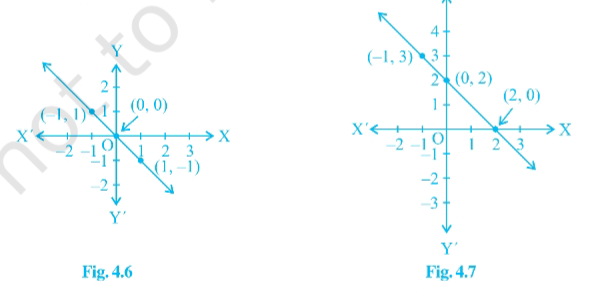
\includegraphics[width=\columnwidth]{chapters/9/figs/4.6-4.7.png}
\caption{Graph}
  \label{fig:4.6-4.7}
\end{figure}
\item If the work done by a body of a constant force is directly proportional 
to the distance travelled by the body,express this in the form of an equation
and draw the graph of the same by taking the varables and draw the graph of 
the same by taking the constant force as $5 units$.Also read from the graph the
work done when the distance travelled by the body is
\begin{enumerate}[label=(\roman*)]
\item $2$Units
\item $0$Unit
\end{enumerate}
\item Yamini and Fatima,two students of class IX of a school,together
 contributed \rupee~100 towards the prime minister's reief fund to help
 the earhquake victims.Write a linear equation which satisfies this data.
 (you may take their contributions  \rupee~x and \rupee~y.Draw the graph 
 of the same.
\item In Countries like USA and Canada temperature is measured in Celsius.
Here is a linear equation that converts Farenheit to celsius:
$F=\frac{9}{5}C+32$
\begin{enumerate}[label=(\roman*)]
\item Draw the graph of the linear equation above using Celsius for $x$
 axis and Farenheit for $y$ axis
\item If the temperature is $30\degree C$,what is the temperature in farenheight?
\item If the temperature is $95\degree F$,what is the temperature in celsius?
\item If the temperature is $0\degree C$.What is the temperature in Farenheit and if the temperature in celsius?
\item Is there a temperature Which is numerically same in both Farenheit and Celsius? If yes find it.
\end{enumerate}
\end{enumerate}

\section{10}
\subsection{Examples:-1-19 (10.3)}
\input{chapters/10/10.3.tex}
\subsection{10.3.1}
\input{chapters/10/10.3.1.tex}
\subsection{10.3.2}
\input{chapters/10/10.3.2.tex}
\subsection{10.3.3}
\begin{enumerate}
\item Solve the following pair of linear equations by the substitution method.
\begin{enumerate}[label=(\roman*)]    
	\item
	\begin{align}
   	 x+y=14 \\x-y=4
	\end{align}
    	\item 
	\begin{align}
	s-t=3
	\end{align}
	\item
	\begin{align}
    	3x-y=3\\ 9x-3y=9
	\end{align}
	\begin{align}   	
 	0.2x+0.3y=1.3\\ 0.4x+0.5y=23
	\end{align}
	\item     
	\begin{align}
	\sqrt{2x}+\sqrt{3y}=0\\ \sqrt{3x}-\sqrt{8y}=0
	\end{align}
	\item
	\begin{align}
    	\frac{3x}{2}-\frac{5y}{2}=-2\\ \frac{x}{3}+\frac{y}{2}=\frac{13}{6}
    	\end{align}
	\end{enumerate}
\item Solve $2x+3y=11$ and $2x+4y=-24$ and hence find the value of $m$ for which $y=mx+3$
\item Form the pair of linear equations for the following problems and find their solutions by the substitution method
    \begin{enumerate}[label=(\Roman*)]
    \item The difference between two numbers is $26$ and one number is three times the other. Find them.
    \item The larger of two supplementary angles exceeds the smaller by $18$ degrees. Find them.
    \item The coach of a cricket team buys $7$ balls and $6$ balls for \rupee~3800. Later, she buys $3$ bats and $5$ balls for \rupee~1750. Find the cost of each bat and each ball.
    \item The taxi charges in a city consist of a fixed charge together with the charges for the distance covered. For a distance of $10$ km, the charge paid is \rupee~105 and for a distance of $15$ km, the charge paid is \rupee~155. What are the fixed charges and the charge per km? How much does a person have to pay for travelling a distance of 25 km ? 
    \item A fraction becomes $\frac{9}{11}$ if $2$ is added to both the numerator and the denominator. If $3$ is added to both the numerator and the denominator, it becomes $\frac{5}{6}$. Find the fraction.
    \item Five years hence, the age of Jacob will be three times that of his son. Five years ago, Jacob's age was seven times that of his son. What are their present ages?
    \end{enumerate}
\end{enumerate}

\subsection{10.3.4}
\input{chapters/10/10.3.4.tex}
\subsection{10.3.5}
\input{chapters/10/10.3.5.tex}
\subsection{10.3.6}
\begin{enumerate}
\item Solve the following pair of equations by reducing them to a pair of linear equations:
\begin{enumerate}[label=(\roman*)]
\item
\begin{align}
\frac{1}{2x}+\frac{1}{3y}=2 \\ \frac{1}{3x}+\frac{1}{2y}=\frac{13}{6}
\end{align}
\item
\begin{align}
\frac{2}{\sqrt{x}}+\frac{3}{\sqrt{y}}=2\\
\frac{4}{\sqrt{x}}-\frac{9}{\sqrt{y}}=-1
\end{align}
\item
\begin{align}
\frac{4}{x}+3y=14\\ \frac{3}{x}-4y=23
\end{align}
\item
\begin{align}
\frac{5}{x-1}+\frac{1}{y-2}=2\\ \frac{6}{x-1}-\frac{3}{y-2}=1
\end{align}
\item
\begin{align}
\frac{7x-2y}{xy}=5\\ \frac{8x+7y}{xy}=15
\end{align}
\item
\begin{align}
6x+3y=6xy\\ 2x+4y=5xy
\end{align}
\item
\begin{align}
\frac{10}{x+y}+\frac{2}{x-y}=4\\ \frac{15}{x+y}-\frac{5}{x-y}=-2
\end{align}
\item
\begin{align}
\frac{1}{3x+y}+\frac{1}{3x-y}=\frac{3}{4}\\ \frac{1}{2(3x+y)}-\frac{1}{2(3x-y)}=\frac{-1}{8}
\end{align}
\end{enumerate}
\item Formulate the following problems as a pair of equations,and hence find their solutions:
\begin{enumerate}[label=(\roman*)]
\item Ritu can row downstream $20km$ in $2$ hours, and upstream $4km$ in $2$ hours. Find her speed of rowing in still water and the speed of the current.
\item $2$ women and $5$ men can together finish an embroidery work in $4$ days, while $3$ women and $6$ men can finish it in $3$ days. Find the time taken by $1$ women along to finish the work, and also that taken by $1$ men alone.
\item Roohi travels $300 km$ to her home partly by train and partly by bus. She takes $4$ hours if she travels $60km$ by train and the remaining by bus. If she travels $100km$ by train and the remaining by bus, she takes $10$ minutes longer. Find the speed of the train and the bus seperately.
\end{enumerate}
\end{enumerate}

\subsection{10.3.7}
\input{chapters/10/10.3.7.tex}
\chapter{Quadratic Equations}
\section{10}
\subsection{Examples:-1-18 (10.4)}                                               
\input{chapters/10/10.4.tex}
\subsection{10.4.1}
\input{chapters/10/10.4.1.tex}
\subsection{10.4.2}
\input{chapters/10/10.4.2.tex}
\subsection{10.4.3}
\input{chapters/10/10.4.3.tex}
\subsection{10.4.4}
\begin{enumerate}
\item Find the nature of the roots of the following quadratic equations. If real roots exist, find them:
\begin{enumerate}[label=(\roman*)]
\item $2x^2-3x+5=0$
\item $3x^2-4 sqrt 3x+4=0$
\item $2x^2-6x+3=0$
\end{enumerate}
\item Find the values of k for each of the following quadratic equations, so that they hav equal roots:
\begin{enumerate}[label=(\roman*)]
\item $2x^2=kx-3=0$
\item $kx(x-2)+6=0$
\end{enumerate}
\item Is it possible to design a rectangular mango grove whose length is twice its breadth, and the area is  $800m^2$? If so, find its length and breadth.
\item Is the following situation possible? If so, determine their present ages.
\\ The sum of the ages of the two friends is 20 years. Four years ago, the product of their ages in years was $48$.
\item Is it possible to design a rectangular park of perimeter 80m and area of $400m^2$. If so, find its length and breadth.
\end{enumerate}



\chapter{Coordinate Geometry}
\section{10}
\subsection{10.7.1}
\input{chapters/10/10.7.1.tex}
\subsection{10.7.2}
\input{chapters/10/10.7.2.tex}
\subsection{10.7.3}
\input{chapters/10/10.7.3.tex}
\subsection{10.7.4}
\input{chapters/10/10.7.4.tex}
\chapter{Straight Lines}
\section{11}
\subsection{11.10.1}
\input{chapters/11/11.10.1.tex}
\subsection{11.10.2}
\input{chapters/11/11.10.2.tex}
\subsection{11.10.3}
\input{chapters/11/11.10.3.tex}
\chapter{Trigonometry}
\section{Ratios}
\input{./chapters/trig/tri_geo_rt}
\section{The Baudhayana Theorem}
\input{./chapters/trig/tri_geo_baudh}
%
\section{Area of a Triangle}
\input{./chapters/trig/tri_geo_sincos}
\section{Angle Bisectors}
\input{./chapters/trig/ang.tex}
\section{Circumradius}
\input{./chapters/trig/tri_geo_cradius}
\section{Tangent}
\input{./chapters/trig/tangent}
\section{Identities}
\input{./chapters/trig/trig_id.tex}
\chapter{Analytic Geometry}
\section{Vectors}
\input{./chapters/coord/vector}
\section{Altitudes of a Triangle:Line Equation}
\input{./chapters/coord/tri_geo_alt}
\section{Circumcircle: Circle Equation}
\input{./chapters/coord/tri_geo_ccentre}
\section{Tangent}
\input{./chapters/coord/circ_geo_prop}
\chapter{Triangle}
\input{./chapters/exercises/tri_geo_exer}
\chapter{Quadrilateral}
\input{./chapters/exercises/quad_geo_exer}
%
\chapter{Circle}
\section{11}
\subsection{11.11.1}
In each of the following exercise \ref{prob:1} to \ref{prob:5}, find the equation of the circle with:
\begin{enumerate}[label=\arabic*.,ref=\thesubsection.\theenumi]
\item centre $(0,2)$ and radius $2$ \label{prob:1}
\item centre $(-2,3)$ and radius $4$
\item centre $\frac({1}{2},\frac{1}{4})$ and radius $\frac {1}{!2}$
\item centre $(1,1)$ and radius $2$
\item centre $(-a,-b)$ and radius $\sqrt{a^2-b^2}$  \label{prob:5}
\end{enumerate}
In each of the following exercise \ref{prob:6} to \ref{prob:9}, find the centre and radius of the circles
\begin{enumerate}[resume]
\item $(x-5)^2+(y-3)^2=36$ \label{prob:6}
\item $x^2+y^2-4x-8y-45=0$
\item $x^2+y^2-8x+10y-12=0$
\item $2x^2+2y^2-x=0$ \label{prob:9}
\end{enumerate}
\begin{enumerate}[resume]
\item Find the equation of the circle passing through the points $(4,1)$ and $(6,5)$ and whose centre is on the line $4x+y=16$.
\item Find the equation of the circle passing through the points $(2,3)$ and $(-1,1)$ and whose centre is on the line $x-3y-11=0$.
\item Find the equation of the circle with radius 5 whose centre lies on x-axis and passes through the point $(2,3)$.
\item Find the equation of the circle passing through $(0,0)$ and making intercepts $a$ and $b$ on the coordinate axes.
\item Find the equation of a circle with centre $(2,2)$ and passes through the point $(4,5)$.
\item Does the point $(-2.5,3.5)$ lie inside, outside or on the circle $x^2+y^2=25$.
\end{enumerate}



\input{./chapters/exercises/circ_geo_exer}
\chapter{Miscellaneous }
\input{./chapters/exercises/geo_misc}
\iffalse
%\include{ch02} 
\backmatter
\appendix
\chapter{Area of a Circle}
\input{./chapters/area/circ_geo_area}
\fi
%
%\chapter{Proofs}
%   \section{}
%\input{apps/defs.tex}

%  \section{}
%\input{apps/parab.tex}
%  \section{}
%\input{apps/nonparab.tex}
%		\section{}
%\input{apps/params.tex}
\latexprintindex

\end{document}

 

		\item Verify that 
		\begin{align}
			OA = OB = OC 
		\end{align}
  \\
  \iffalse
\documentclass{article}
\title{Assignment-1}
\author{Chaithanya - EE22BTECH11045}
\usepackage{amsmath}
\usepackage{amssymb}
\usepackage{graphicx}
\usepackage{hyperref}
\begin{document}
\providecommand{\pr}[1]{\ensuremath{\Pr\left(#1\right)}}
\providecommand{\prt}[2]{\ensuremath{p_{#1}^{\left(#2\right)} }}        % own macro for this question
\providecommand{\qfunc}[1]{\ensuremath{Q\left(#1\right)}}
\providecommand{\sbrak}[1]{\ensuremath{{}\left[#1\right]}}
\providecommand{\lsbrak}[1]{\ensuremath{{}\left[#1\right.}}
\providecommand{\rsbrak}[1]{\ensuremath{{}\left.#1\right]}}
\providecommand{\brak}[1]{\ensuremath{\left(#1\right)}}
\providecommand{\lbrak}[1]{\ensuremath{\left(#1\right.}}
\providecommand{\rbrak}[1]{\ensuremath{\left.#1\right)}}
\providecommand{\cbrak}[1]{\ensuremath{\left\{#1\right\}}}
\providecommand{\lcbrak}[1]{\ensuremath{\left\{#1\right.}}
\providecommand{\rcbrak}[1]{\ensuremath{\left.#1\right\}}}
\newcommand{\sgn}{\mathop{\mathrm{sgn}}}
\providecommand{\abs}[1]{\left\vert#1\right\vert}
\providecommand{\res}[1]{\Res\displaylimits_{#1}} 
\providecommand{\norm}[1]{\left\lVert#1\right\rVert}
%\providecommand{\norm}[1]{\lVert#1\rVert}
\providecommand{\mtx}[1]{\mathbf{#1}}
\providecommand{\mean}[1]{E\left[ #1 \right]}
\providecommand{\cond}[2]{#1\middle|#2}
\providecommand{\fourier}{\overset{\mathcal{F}}{ \rightleftharpoons}}
\newenvironment{amatrix}[1]{%
  \left(\begin{array}{@{}*{#1}{c}|c@{}}
}{%
  \end{array}\right)
}
%\providecommand{\hilbert}{\overset{\mathcal{H}}{ \rightleftharpoons}}
%\providecommand{\system}{\overset{\mathcal{H}}{ \longleftrightarrow}}
	%\newcommand{\solution}[2]{\textbf{Solution:}{#1}}
\newcommand{\solution}{\noindent \textbf{Solution: }}
\newcommand{\cosec}{\,\text{cosec}\,}
\providecommand{\dec}[2]{\ensuremath{\overset{#1}{\underset{#2}{\gtrless}}}}
\newcommand{\myvec}[1]{\ensuremath{\begin{pmatrix}#1\end{pmatrix}}}
\newcommand{\mydet}[1]{\ensuremath{\begin{vmatrix}#1\end{vmatrix}}}
\newcommand{\myaugvec}[2]{\ensuremath{\begin{amatrix}{#1}#2\end{amatrix}}}
\providecommand{\rank}{\text{rank}}
\providecommand{\pr}[1]{\ensuremath{\Pr\left(#1\right)}}
\providecommand{\qfunc}[1]{\ensuremath{Q\left(#1\right)}}
	\newcommand*{\permcomb}[4][0mu]{{{}^{#3}\mkern#1#2_{#4}}}
\newcommand*{\perm}[1][-3mu]{\permcomb[#1]{P}}
\newcommand*{\comb}[1][-1mu]{\permcomb[#1]{C}}
\providecommand{\qfunc}[1]{\ensuremath{Q\left(#1\right)}}
\providecommand{\gauss}[2]{\mathcal{N}\ensuremath{\left(#1,#2\right)}}
\providecommand{\diff}[2]{\ensuremath{\frac{d{#1}}{d{#2}}}}
\providecommand{\myceil}[1]{\left \lceil #1 \right \rceil }
\newcommand\figref{Fig.~\ref}
\newcommand\tabref{Table~\ref}
\newcommand{\sinc}{\,\text{sinc}\,}
\newcommand{\rect}{\,\text{rect}\,}
%%
%	%\newcommand{\solution}[2]{\textbf{Solution:}{#1}}
%\newcommand{\solution}{\noindent \textbf{Solution: }}
%\newcommand{\cosec}{\,\text{cosec}\,}
%\numberwithin{equation}{section}
%\numberwithin{equation}{subsection}
%\numberwithin{problem}{section}
%\numberwithin{definition}{section}
%\makeatletter
%\@addtoreset{figure}{problem}
%\makeatother

%\let\StandardTheFigure\thefigure
\let\vec\mathbf
\maketitle
\noindent \textbf{1.4.4} Verify that
\begin{align}
OA = OB = OC
\end{align}
\fi
\solution
Given \begin{align}
\vec{A} &= \myvec{1\\-1}\\
\vec{B} &= \myvec{-4\\6}\\
\vec{C} &= \myvec{-3\\-5}
\end{align}
From problem-1.4.2 :
\begin{align}
O &= \myvec{\frac{-53}{12} \\ \frac{-5}{12}}\\
 &= \myvec{-4.4167\\ 0.4167}
\end{align}
\begin{enumerate}
\item 
\begin{align}
OA &= \sqrt{(\vec{O}-\vec{A})^{\top}(\vec{O}-\vec{A})}\\
&= \sqrt{\myvec{-5.4167 & 1.4167} \myvec{-5.4167\\1.4167}}\\
 &= \sqrt{31.3476}\\
 &= 5.5988
\end{align}
\item 
\begin{align}
OB &= \sqrt{(\vec{O}-\vec{B})^{\top}(\vec{O}-\vec{B})}\\
 &= \sqrt{\myvec{-0.4167 & -5.5833} \myvec{-0.4167\\-5.5833}}\\
 &= \sqrt{31.3468}\\
 &= 5.5988
\end{align}
\item 
\begin{align}
OC &= \sqrt{(\vec{O}-\vec{C})^{\top}(\vec{O}-\vec{C})}\\
 &= \sqrt{\myvec{-1.4167 & 5.4167}  \myvec{-1.4167\\5.4167}}\\
&= \sqrt{31.3476}\\
 &= 5.5988
\end{align}
\end{enumerate}
From above, 
\begin{align}
OA = OB = OC
\end{align}
Hence verified.

  \iffalse
\documentclass{article}
\title{Assignment-1}
\author{Chaithanya - EE22BTECH11045}
\usepackage{amsmath}
\usepackage{amssymb}
\usepackage{graphicx}
\usepackage{hyperref}
\begin{document}
\providecommand{\pr}[1]{\ensuremath{\Pr\left(#1\right)}}
\providecommand{\prt}[2]{\ensuremath{p_{#1}^{\left(#2\right)} }}        % own macro for this question
\providecommand{\qfunc}[1]{\ensuremath{Q\left(#1\right)}}
\providecommand{\sbrak}[1]{\ensuremath{{}\left[#1\right]}}
\providecommand{\lsbrak}[1]{\ensuremath{{}\left[#1\right.}}
\providecommand{\rsbrak}[1]{\ensuremath{{}\left.#1\right]}}
\providecommand{\brak}[1]{\ensuremath{\left(#1\right)}}
\providecommand{\lbrak}[1]{\ensuremath{\left(#1\right.}}
\providecommand{\rbrak}[1]{\ensuremath{\left.#1\right)}}
\providecommand{\cbrak}[1]{\ensuremath{\left\{#1\right\}}}
\providecommand{\lcbrak}[1]{\ensuremath{\left\{#1\right.}}
\providecommand{\rcbrak}[1]{\ensuremath{\left.#1\right\}}}
\newcommand{\sgn}{\mathop{\mathrm{sgn}}}
\providecommand{\abs}[1]{\left\vert#1\right\vert}
\providecommand{\res}[1]{\Res\displaylimits_{#1}} 
\providecommand{\norm}[1]{\left\lVert#1\right\rVert}
%\providecommand{\norm}[1]{\lVert#1\rVert}
\providecommand{\mtx}[1]{\mathbf{#1}}
\providecommand{\mean}[1]{E\left[ #1 \right]}
\providecommand{\cond}[2]{#1\middle|#2}
\providecommand{\fourier}{\overset{\mathcal{F}}{ \rightleftharpoons}}
\newenvironment{amatrix}[1]{%
  \left(\begin{array}{@{}*{#1}{c}|c@{}}
}{%
  \end{array}\right)
}
%\providecommand{\hilbert}{\overset{\mathcal{H}}{ \rightleftharpoons}}
%\providecommand{\system}{\overset{\mathcal{H}}{ \longleftrightarrow}}
	%\newcommand{\solution}[2]{\textbf{Solution:}{#1}}
\newcommand{\solution}{\noindent \textbf{Solution: }}
\newcommand{\cosec}{\,\text{cosec}\,}
\providecommand{\dec}[2]{\ensuremath{\overset{#1}{\underset{#2}{\gtrless}}}}
\newcommand{\myvec}[1]{\ensuremath{\begin{pmatrix}#1\end{pmatrix}}}
\newcommand{\mydet}[1]{\ensuremath{\begin{vmatrix}#1\end{vmatrix}}}
\newcommand{\myaugvec}[2]{\ensuremath{\begin{amatrix}{#1}#2\end{amatrix}}}
\providecommand{\rank}{\text{rank}}
\providecommand{\pr}[1]{\ensuremath{\Pr\left(#1\right)}}
\providecommand{\qfunc}[1]{\ensuremath{Q\left(#1\right)}}
	\newcommand*{\permcomb}[4][0mu]{{{}^{#3}\mkern#1#2_{#4}}}
\newcommand*{\perm}[1][-3mu]{\permcomb[#1]{P}}
\newcommand*{\comb}[1][-1mu]{\permcomb[#1]{C}}
\providecommand{\qfunc}[1]{\ensuremath{Q\left(#1\right)}}
\providecommand{\gauss}[2]{\mathcal{N}\ensuremath{\left(#1,#2\right)}}
\providecommand{\diff}[2]{\ensuremath{\frac{d{#1}}{d{#2}}}}
\providecommand{\myceil}[1]{\left \lceil #1 \right \rceil }
\newcommand\figref{Fig.~\ref}
\newcommand\tabref{Table~\ref}
\newcommand{\sinc}{\,\text{sinc}\,}
\newcommand{\rect}{\,\text{rect}\,}
%%
%	%\newcommand{\solution}[2]{\textbf{Solution:}{#1}}
%\newcommand{\solution}{\noindent \textbf{Solution: }}
%\newcommand{\cosec}{\,\text{cosec}\,}
%\numberwithin{equation}{section}
%\numberwithin{equation}{subsection}
%\numberwithin{problem}{section}
%\numberwithin{definition}{section}
%\makeatletter
%\@addtoreset{figure}{problem}
%\makeatother

%\let\StandardTheFigure\thefigure
\let\vec\mathbf
\maketitle
\noindent \textbf{1.4.4} Verify that
\begin{align}
OA = OB = OC
\end{align}
\fi
\solution
Given \begin{align}
\vec{A} &= \myvec{1\\-1}\\
\vec{B} &= \myvec{-4\\6}\\
\vec{C} &= \myvec{-3\\-5}
\end{align}
From problem-1.4.2 :
\begin{align}
O &= \myvec{\frac{-53}{12} \\ \frac{-5}{12}}\\
 &= \myvec{-4.4167\\ 0.4167}
\end{align}
\begin{enumerate}
\item 
\begin{align}
OA &= \sqrt{(\vec{O}-\vec{A})^{\top}(\vec{O}-\vec{A})}\\
&= \sqrt{\myvec{-5.4167 & 1.4167} \myvec{-5.4167\\1.4167}}\\
 &= \sqrt{31.3476}\\
 &= 5.5988
\end{align}
\item 
\begin{align}
OB &= \sqrt{(\vec{O}-\vec{B})^{\top}(\vec{O}-\vec{B})}\\
 &= \sqrt{\myvec{-0.4167 & -5.5833} \myvec{-0.4167\\-5.5833}}\\
 &= \sqrt{31.3468}\\
 &= 5.5988
\end{align}
\item 
\begin{align}
OC &= \sqrt{(\vec{O}-\vec{C})^{\top}(\vec{O}-\vec{C})}\\
 &= \sqrt{\myvec{-1.4167 & 5.4167}  \myvec{-1.4167\\5.4167}}\\
&= \sqrt{31.3476}\\
 &= 5.5988
\end{align}
\end{enumerate}
From above, 
\begin{align}
OA = OB = OC
\end{align}
Hence verified.

	\item Draw the circle with centre at $\vec{O}$ and radius 
		\begin{align}
			R = OA
		\end{align}
		This is known as the {\em circumradius}. 
  \\  \input{solutions/1/4/5/assignment2.tex}
	\item Verify that 
		\begin{align}
			\angle BOC = 2\angle BAC.
		\end{align}\\
  \input{solutions/1/4/6/Q_1.4.6.tex}
	\item Let 
		\begin{align}
			\vec{P} = \myvec{\cos \theta & -\sin \theta \\ \sin \theta & \cos \theta}
		\end{align}
		Find $\theta$ if 
		\begin{align}
			\vec{C}-\vec{O}=\vec{P}\brak{\vec{A}-\vec{O}}
		\end{align}
\end{enumerate}

\section{Angle Bisector}
%\renewcommand{\theequation}{\theenumi}
%\begin{enumerate}[label=\arabic*.,ref=\theenumi]
\begin{enumerate}[label=\thesection.\arabic*.,ref=\thesection.\theenumi]
\numberwithin{equation}{enumi}
\item Suppose the equations $AB, BC$ and $CA$ are respectively given by 
		\begin{align}
			\label{eq:tri-sides}
			\vec{n}_i^{\top}\vec{x}=c_i \quad i = 1, 2, 3 
		\end{align}
		The equations of the respective angle bisectors are then given by 
		\begin{align}
			\frac{\vec{n}_i^{\top}\vec{x}-c_i}{\norm{\vec{n}_i}}
		=
	\pm	\frac{\vec{n}_j^{\top}\vec{x}-c_j}{\norm{\vec{n}_j}}
\quad i \ne j
		\end{align}
		Substitute numerical values and find the equations of the angle bisectors of $A, B$ and $C$.
	\\
		%\input{solutions/1/5/1/Assignment_1.tex}
  %% Run LaTeX on this file several times to get Table of Contents,
%% cross-references, and citations.

\documentclass[11pt]{book}
\usepackage{gvv-book}
\usepackage{gvv}
%\usepackage{Wiley-AuthoringTemplate}
\usepackage[sectionbib,authoryear]{natbib}% for name-date citation comment the below line
%\usepackage[sectionbib,numbers]{natbib}% for numbered citation comment the above line

%%********************************************************************%%
%%       How many levels of section head would you like numbered?     %%
%% 0= no section numbers, 1= section, 2= section, 3= subsection %%
\setcounter{secnumdepth}{3}
%%********************************************************************%%
%%**********************************************************************%%
%%     How many levels of section head would you like to appear in the  %%
%%				Table of Contents?			%%
%% 0= chapter, 1= section, 2= section, 3= subsection titles.	%%
\setcounter{tocdepth}{2}
%%**********************************************************************%%

%\includeonly{ch01}
\makeindex

\begin{document}

\frontmatter
%%%%%%%%%%%%%%%%%%%%%%%%%%%%%%%%%%%%%%%%%%%%%%%%%%%%%%%%%%%%%%%%
%% Title Pages
%% Wiley will provide title and copyright page, but you can make
%% your own titlepages if you'd like anyway
%% Setting up title pages, type in the appropriate names here:

\booktitle{Geometry}

\subtitle{Through Algebra}

\AuAff{G. V. V. Sharma}


%% \\ will start a new line.
%% You may add \affil{} for affiliation, ie,
%\authors{Robert M. Groves\\
%\affil{Universitat de les Illes Balears}
%Floyd J. Fowler, Jr.\\
%\affil{University of New Mexico}
%}

%% Print Half Title and Title Page:
%\halftitlepage
\titlepage

%%%%%%%%%%%%%%%%%%%%%%%%%%%%%%%%%%%%%%%%%%%%%%%%%%%%%%%%%%%%%%%%
%% Copyright Page

\begin{copyrightpage}{2022}
%Title, etc
\end{copyrightpage}

% Note, you must use \ to start indented lines, ie,
% 
% \begin{copyrightpage}{2004}
% Survey Methodology / Robert M. Groves . . . [et al.].
% \       p. cm.---(Wiley series in survey methodology)
% \    ``Wiley-Interscience."
% \    Includes bibliographical references and index.
% \    ISBN 0-471-48348-6 (pbk.)
% \    1. Surveys---Methodology.  2. Social 
% \  sciences---Research---Statistical methods.  I. Groves, Robert M.  II. %
% Series.\\

% HA31.2.S873 2004
% 001.4'33---dc22                                             2004044064
% \end{copyrightpage}

%%%%%%%%%%%%%%%%%%%%%%%%%%%%%%%%%%%%%%%%%%%%%%%%%%%%%%%%%%%%%%%%
%% Only Dedication (optional) 

%\dedication{To my parents}

\tableofcontents

%\listoffigures %optional
%\listoftables  %optional

%% or Contributor Page for edited books
%% before \tableofcontents

%%%%%%%%%%%%%%%%%%%%%%%%%%%%%%%%%%%%%%%%%%%%%%%%%%%%%%%%%%%%%%%%
%  Contributors Page for Edited Book
%%%%%%%%%%%%%%%%%%%%%%%%%%%%%%%%%%%%%%%%%%%%%%%%%%%%%%%%%%%%%%%%

% If your book has chapters written by different authors,
% you'll need a Contributors page.

% Use \begin{contributors}...\end{contributors} and
% then enter each author with the \name{} command, followed
% by the affiliation information.

% \begin{contributors}
% \name{Masayki Abe,} Fujitsu Laboratories Ltd., Fujitsu Limited, Atsugi, Japan
%
% \name{L. A. Akers,} Center for Solid State Electronics Research, Arizona State University, Tempe, Arizona
%
% \name{G. H. Bernstein,} Department of Electrical and Computer Engineering, University of Notre Dame, Notre Dame, South Bend, Indiana; formerly of
% Center for Solid State Electronics Research, Arizona
% State University, Tempe, Arizona 
% \end{contributors}

%%%%%%%%%%%%%%%%%%%%%%%%%%%%%%%%%%%%%%%%%%%%%%%%%%%%%%%%%%%%%%%%
% Optional Foreword:

%\begin{foreword}
%\lipsum[1-2]
%\end{foreword}

%%%%%%%%%%%%%%%%%%%%%%%%%%%%%%%%%%%%%%%%%%%%%%%%%%%%%%%%%%%%%%%%
% Optional Preface:

%\begin{preface}
%\lipsum[1-1]
%\prefaceauthor{}
%\where{place\\
% date}
%\end{preface}

% ie,
% \begin{preface}
% This is an example preface.
% \prefaceauthor{R. K. Watts}
% \where{Durham, North Carolina\\
% September, 2004}

%%%%%%%%%%%%%%%%%%%%%%%%%%%%%%%%%%%%%%%%%%%%%%%%%%%%%%%%%%%%%%%%
% Optional Acknowledgments:

%\acknowledgments
%\lipsum[1-2]
%\authorinitials{I. R. S.}  

%%%%%%%%%%%%%%%%%%%%%%%%%%%%%%%%
%% Glossary Type of Environment:

% \begin{glossary}
% \term{<term>}{<description>}
% \end{glossary}

%%%%%%%%%%%%%%%%%%%%%%%%%%%%%%%%
%\begin{acronyms}
%\acro{ASTA}{Arrivals See Time Averages}
%\acro{BHCA}{Busy Hour Call Attempts}
%\acro{BR}{Bandwidth Reservation}
%\acro{b.u.}{bandwidth unit(s)}
%\acro{CAC}{Call / Connection Admission Control}
%\acro{CBP}{Call Blocking Probability(-ies)}
%\acro{CCS}{Centum Call Seconds}
%\acro{CDTM}{Connection Dependent Threshold Model}
%\acro{CS}{Complete Sharing}
%\acro{DiffServ}{Differentiated Services}
%\acro{EMLM}{Erlang Multirate Loss Model}
%\acro{erl}{The Erlang unit of traffic-load}
%\acro{FIFO}{First in - First out}
%\acro{GB}{Global balance}
%\acro{GoS}{Grade of Service}
%\acro{ICT}{Information and Communication Technology}
%\acro{IntServ}{Integrated Services}
%\acro{IP}{Internet Protocol}
%\acro{ITU-T}{International Telecommunication Unit -- Standardization sector}
%\acro{LB}{Local balance}
%\acro{LHS}{Left hand side}
%\acro{LIFO}{Last in - First out}
%\acro{MMPP}{Markov Modulated Poisson Process}
%\acro{MPLS}{Multiple Protocol Labeling Switching}
%\acro{MRM}{Multi-Retry Model}
%\acro{MTM}{Multi-Threshold Model}
%\acro{PASTA}{Poisson Arrivals See Time Averages}
%\acro{PDF}{Probability Distribution Function}
%\acro{pdf}{probability density function}
%\acro{PFS}{Product Form Solution}
%\acro{QoS}{Quality of Service}
%\acro{r.v.}{random variable(s)}
%\acro{RED}{random early detection}
%\acro{RHS}{Right hand side}
%\acro{RLA}{Reduced Load Approximation}
%\acro{SIRO}{service in random order}
%\acro{SRM}{Single-Retry Model}
%\acro{STM}{Single-Threshold Model}
%\acro{TCP}{Transport Control Protocol}
%\acro{TH}{Threshold(s)}
%\acro{UDP}{User Datagram Protocol}
%\end{acronyms}

\setcounter{page}{1}

\begin{introduction}
This book shows how to solve problems in geometry using trigonometry and coordinate geometry. 

\end{introduction}

\mainmatter

\chapter{Triangle}
Consider a triangle with vertices
		\begin{align}
			\label{eq:tri-pts}
			\vec{A} = \myvec{1 \\ -1},\,
			\vec{B} = \myvec{-4 \\ 6},\,
			\vec{C} = \myvec{-3 \\ -5}
		\end{align}
\section{Vectors}
%\renewcommand{\theequation}{\theenumi}
%\begin{enumerate}[label=\arabic*.,ref=\theenumi]
\begin{enumerate}[label=\thesection.\arabic*.,ref=\thesection.\theenumi]
\numberwithin{equation}{enumi}
\item The direction vector of $AB$ is defined as
		\begin{align}
			\vec{B}-
			\vec{A}
		\end{align}
Find the direction vectors of $AB, BC$ and $CA$.
\\
	\input{solutions/1/1/1/prob_1.tex}
	\item The length of side $BC$ is 
		\begin{align}
			\norm{\vec{B}-\vec{A}} \triangleq \sqrt{\brak{\vec{B}-\vec{A}}^{\top}{\vec{B}-\vec{A}}}
		\end{align}
		where
		\begin{align}
			\vec{A}^{\top}\triangleq\myvec{1 & -1}
		\end{align}
  \\		\input{solutions/1/1/2/main.tex}
\item   Points $\vec{A}, \vec{B}, \vec{C}$ are defined to be collinear if 
		\begin{align}
			\rank{\myvec{1 & 1 & 1 \\ \vec{A}& \vec{B}&\vec{C}}} = 2
		\end{align}
Are the given points in
			\eqref{eq:tri-pts}
collinear?\\
\input{solutions/1/1/3/main.tex}
\item The parameteric form of the equation  of $AB$ is 
		\begin{align}
			\vec{x}=\vec{A}+k\vec{m}
		\end{align}
		where
		\begin{align}
\vec{m}=\vec{B}-\vec{A}
		\end{align}
is the direction vector of $AB$.
Find the parameteric equations of $AB, BC$ and $CA$.
\\
		\input{solutions/1/1/4/main.tex}
\item The normal form of the equation of $AB$  is 
		\begin{align}
			\vec{n}^{\top}\brak{	\vec{x}-\vec{A}} = 0
		\end{align}
		where 
		\begin{align}
			\vec{n}^{\top}\vec{m}&=\vec{n}^{\top}\brak{\vec{B}-\vec{A}} = 0
			\\
			\text{or, } \vec{n}&=\myvec{0 & 1 \\ -1 & 0} \vec{m}
		\end{align}
Find the normal form of the equations of $AB, BC$ and $CA$.
\input{solutions/1/1/5/assign1.tex}
\input{solutions/1/1/5a/assignment1.tex}
\input{solutions/1/1/5c/main.tex}
\item The area of $\triangle ABC$ is defined as
		\begin{align}
			\frac{1}{2}\norm{{\brak{\vec{A}-\vec{B}}\times {\vec{A}-\vec{C}}}}
		\end{align}
		where
		\begin{align}
			\vec{A}\times\vec{B} \triangleq \mydet{1 & -4 \\-1 & 6}
		\end{align}
		Find the area of $\triangle ABC$.\\
  		\input{solutions/1/1/6/main.tex}
	\item Find the angles $A, B, C$ if 
    \label{prop:angle2d}
  \begin{align}
    \label{eq:angle2d}
			\cos A \triangleq 
\frac{\brak{\vec{B}-\vec{A}}^{\top}{\vec{C}-\vec{A}}}{\norm{\vec{B}-\vec{A}}\norm{\vec{C}-\vec{A}}}
  \end{align}\\
  	\input{solutions/1/1/7/main.tex}
\end{enumerate}

\section{Median}
%\renewcommand{\theequation}{\theenumi}
%\begin{enumerate}[label=\arabic*.,ref=\theenumi]
\begin{enumerate}[label=\thesection.\arabic*.,ref=\thesection.\theenumi]
\numberwithin{equation}{enumi}
\item If $\vec{D}$ divides $BC$ in the ratio $k : 1$,
		\begin{align}
			\vec{D}= \frac{k\vec{C}+\vec{B}}{k+1}
		\end{align}
		Find the mid points $\vec{D}, \vec{E}, \vec{F}$ of the sides $BC, CA$ and $AB$ respectively.
		\\
			\input{solutions/1/2/1/main.tex} 
	\item Find the equations of $AD, BE$ and $CF$.
	\item Find the intersection $\vec{G}$ of $BE$ and $CF$.
	\item Verify that 
		\begin{align}
			\frac{BG}{GE} = 
			\frac{CG}{GF} =
			\frac{AG}{GD} =2 
		\end{align}
	\item Show that $\vec{A}, \vec{G}$ and $\vec{D}$ are collinear.
	\item Verify that 
		\begin{align}
			\vec{G}=\frac{\vec{A}+\vec{B}+\vec{C}}{3}
		\end{align}
			$\vec{G}$ is known as the {\em centroid} of $\triangle ABC$.
   \\
		\input{solutions/1/2/6/main.tex}
	\item Verify that 
		\begin{align}
\vec{A}-\vec{F}=\vec{E}-\vec{D}
		\end{align}
		The quadrilateral $AFDE$ is defined to be a parallelogram.
\end{enumerate}

\section{Altitude}
%\renewcommand{\theequation}{\theenumi}
%\begin{enumerate}[label=\arabic*.,ref=\theenumi]
\begin{enumerate}[label=\thesection.\arabic*.,ref=\thesection.\theenumi]
\numberwithin{equation}{enumi}
\item $\vec{D}_1$ is a point on $BC$ such that
		\begin{align}
			AD_1 \perp BC
		\end{align}
		and $AD_1$ is defined to be the altitude. 
		Find the normal vector of $AD_1$.
  \\
		\input{solutions/1/3/1/main.tex}
	\item Find the equation of $AD_1$.

	\item Find the equations of the altitudes $BE_1$ and $CF_1$ to the sides $AC$ and $AB$ respectively. 
	\item Find the intersection $\vec{H}$ of $BE_1$ and $CF_1$.
	\item Verify that 
		\begin{align}
			\brak{\vec{A}-\vec{H}}^{\top}\brak{\vec{B}-\vec{C}} = 0
		\end{align}
  \\
  	\input{solutions/1/3/5/main.tex}
\end{enumerate}

\section{Perpendicular Bisector}
%\renewcommand{\theequation}{\theenumi}
%\begin{enumerate}[label=\arabic*.,ref=\theenumi]
\begin{enumerate}[label=\thesection.\arabic*.,ref=\thesection.\theenumi]
\numberwithin{equation}{enumi}

\item The equation of the perpendicular bisector of $BC$ is
		\begin{align}
			\label{eq:tri-perp-bisect}
			\brak{\vec{x}-\frac{\vec{B}+\vec{C}}{2}}\brak{\vec{B}-\vec{C}} = 0
		\end{align}
		Substitute numerical values and find the equations of the perpendicular bisectors of $AB, BC$ and $CA$.
	\\	\input{solutions/1/4/1/q1.4.1.tex}
	\item Find the intersection $\vec{O}$ of the perpendicular bisectors of $AB$ and $AC$.
 \\
 \input{solutions/1/4/2/main.tex}
	\item Verify that $\vec{O}$ satisfies
			\eqref{eq:tri-perp-bisect}.
$\vec{O}$ is known as the circumcentre.\\
   \input{solutions/1/4/3/main.tex}
		\item Verify that 
		\begin{align}
			OA = OB = OC 
		\end{align}
  \\
  \input{solutions/1/4/4/main.tex}
  \input{solutions/1/4/4(1)/main.tex}
	\item Draw the circle with centre at $\vec{O}$ and radius 
		\begin{align}
			R = OA
		\end{align}
		This is known as the {\em circumradius}. 
  \\  \input{solutions/1/4/5/assignment2.tex}
	\item Verify that 
		\begin{align}
			\angle BOC = 2\angle BAC.
		\end{align}\\
  \input{solutions/1/4/6/Q_1.4.6.tex}
	\item Let 
		\begin{align}
			\vec{P} = \myvec{\cos \theta & -\sin \theta \\ \sin \theta & \cos \theta}
		\end{align}
		Find $\theta$ if 
		\begin{align}
			\vec{C}-\vec{O}=\vec{P}\brak{\vec{A}-\vec{O}}
		\end{align}
\end{enumerate}

\section{Angle Bisector}
%\renewcommand{\theequation}{\theenumi}
%\begin{enumerate}[label=\arabic*.,ref=\theenumi]
\begin{enumerate}[label=\thesection.\arabic*.,ref=\thesection.\theenumi]
\numberwithin{equation}{enumi}
\item Suppose the equations $AB, BC$ and $CA$ are respectively given by 
		\begin{align}
			\label{eq:tri-sides}
			\vec{n}_i^{\top}\vec{x}=c_i \quad i = 1, 2, 3 
		\end{align}
		The equations of the respective angle bisectors are then given by 
		\begin{align}
			\frac{\vec{n}_i^{\top}\vec{x}-c_i}{\norm{\vec{n}_i}}
		=
	\pm	\frac{\vec{n}_j^{\top}\vec{x}-c_j}{\norm{\vec{n}_j}}
\quad i \ne j
		\end{align}
		Substitute numerical values and find the equations of the angle bisectors of $A, B$ and $C$.
	\\
		%\input{solutions/1/5/1/Assignment_1.tex}
  \input{solutions/1/5/1(1)/main.tex}
	\item Find the intersection $\vec{I}$ of the angle bisectors of $B$ and $C$.
 \\
		\input{solutions/1/5/2/main.tex}
	\item Using 
    \eqref{eq:angle2d}
verify that 
		\begin{align}
			\angle BAI = \angle CAI.
		\end{align}
	\item Find the distance from $\vec{I}$ to $BC$.  \\
        \input{solutions/1/5/4/main.tex}
	\item Repeat the above exercise for the sides $AB$ and $AC$.
	\item This distance is known as the {\em inradius} $r$.
	\item Draw a circle with center $\vec{I}$ and radius $r$.  $\vec{I}$ is known as the {\em incentre}.
	\item The equation of the {\em incircle} is given by 
		\begin{align}
			\norm{\vec{x}-\vec{I}}^2 = r^2
		\end{align}
		Find the parameteric equation of $BC$ and use it to verify that $BC$ intersects the incircle at exactly one point $\vec{D}_3$.  $BC$ is defined to be a {\em tangent} to the incircle.  $\vec{D}_3$ is defined to be {\em point of contact}.
	\\
		\input{solutions/1/5/8/main.tex}
  \item Find the other points of contact $\vec{E}_3$ and $\vec{F}_3$.
	\item Verify that 
		\begin{align}
			AE_3 = AF_3=m, BD_3 = BF_3=n, CD_3 = CE_3=p.
		\end{align}
	\item Obtain $m,n,p$ in terms of $a,b,c$, the sides of the triangle using a matrix equation.  Obtain the numerical values.
 \\
 		\input{solutions/1/5/11/main.tex}
\end{enumerate}

%
\chapter{Linear Equations}
\section{9}
\subsection{9.3.3}
\input{chapters/9/9.3.3.tex}
\subsection{9.4.1}
\begin{enumerate}[label=\arabic*.,ref=\theenumi]
\item The cost of a notebook is twice the cost of a pen.Write a linear
equation in two variables to represent this statement.
(Take the Cost of a notebook to be $x$ and that of a pen to be
$y$).
\item Express the following linear equation in the form $ax+by+c=0$
and indicate the values of $a,b$ and $c$ in each case:
%\begin{enumerate}
\begin{enumerate}[label=(\roman*),ref=\theenumi]
\item $2x+3y=9.3\overline{5}$
\item $x-\frac{y}{5}-10=10$
\item $-2x+3y=6$
\item $ x=3y$
\item $2x=-5y$
\item $3x+2=0$
\item $y-2=0$
\item $5=2x$
\end{enumerate}
\end{enumerate}

\subsection{9.4.2}
\input{chapters/9/9.4.2.tex}
\subsection{9.4.3}
\begin{enumerate}[label=\arabic*.,ref=\theenumi]
\item Draw the graph of each of the following linear equations in two variables:
\begin{enumerate}[label=(\roman*),ref=\theenumi]
\item $x+y=4$
\item $x-y=2$
\item $y=3x$
\item $3=2x+y$
\end{enumerate}
\item Give the equations of two lines passing through (2,14).How many more such lines are there and 
why?
\item If the point(3,4) lies on the graph of the equation $3y=ax+7$ find the value of a
\item The taxi fare in the city is as follows:for te first kilometre,the fare is \rupee~8 and for the 
subsquent distance is \rupee~5 per km.Taking the distance Covered as $x$ km and total fare as
\rupee~y.Write a linear equation for this information,and draw its graph.
\item From the choices given below,choose the equation whose graphs are given Fig 4.6 Fig 4.7
\\
For fig-4.6 
\begin{enumerate}[label=(\roman*)]
\item $y=x$
\item $x+y=0$
\item $y=2x$
\item $2+3y=7x$
\end{enumerate} 
For fig-4.7 
\begin{enumerate}[label=(\roman*)]
\item $y=x+2$
\item $y=x-2$
\item $y=-x+2$
\item $x+2y=6$
\end{enumerate}
\begin{figure}[ht]
\centering
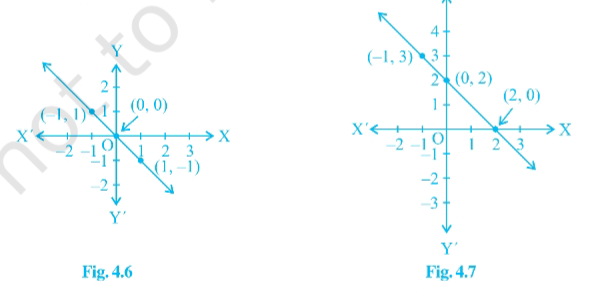
\includegraphics[width=\columnwidth]{chapters/9/figs/4.6-4.7.png}
\caption{Graph}
  \label{fig:4.6-4.7}
\end{figure}
\item If the work done by a body of a constant force is directly proportional 
to the distance travelled by the body,express this in the form of an equation
and draw the graph of the same by taking the varables and draw the graph of 
the same by taking the constant force as $5 units$.Also read from the graph the
work done when the distance travelled by the body is
\begin{enumerate}[label=(\roman*)]
\item $2$Units
\item $0$Unit
\end{enumerate}
\item Yamini and Fatima,two students of class IX of a school,together
 contributed \rupee~100 towards the prime minister's reief fund to help
 the earhquake victims.Write a linear equation which satisfies this data.
 (you may take their contributions  \rupee~x and \rupee~y.Draw the graph 
 of the same.
\item In Countries like USA and Canada temperature is measured in Celsius.
Here is a linear equation that converts Farenheit to celsius:
$F=\frac{9}{5}C+32$
\begin{enumerate}[label=(\roman*)]
\item Draw the graph of the linear equation above using Celsius for $x$
 axis and Farenheit for $y$ axis
\item If the temperature is $30\degree C$,what is the temperature in farenheight?
\item If the temperature is $95\degree F$,what is the temperature in celsius?
\item If the temperature is $0\degree C$.What is the temperature in Farenheit and if the temperature in celsius?
\item Is there a temperature Which is numerically same in both Farenheit and Celsius? If yes find it.
\end{enumerate}
\end{enumerate}

\section{10}
\subsection{Examples:-1-19 (10.3)}
\input{chapters/10/10.3.tex}
\subsection{10.3.1}
\input{chapters/10/10.3.1.tex}
\subsection{10.3.2}
\input{chapters/10/10.3.2.tex}
\subsection{10.3.3}
\begin{enumerate}
\item Solve the following pair of linear equations by the substitution method.
\begin{enumerate}[label=(\roman*)]    
	\item
	\begin{align}
   	 x+y=14 \\x-y=4
	\end{align}
    	\item 
	\begin{align}
	s-t=3
	\end{align}
	\item
	\begin{align}
    	3x-y=3\\ 9x-3y=9
	\end{align}
	\begin{align}   	
 	0.2x+0.3y=1.3\\ 0.4x+0.5y=23
	\end{align}
	\item     
	\begin{align}
	\sqrt{2x}+\sqrt{3y}=0\\ \sqrt{3x}-\sqrt{8y}=0
	\end{align}
	\item
	\begin{align}
    	\frac{3x}{2}-\frac{5y}{2}=-2\\ \frac{x}{3}+\frac{y}{2}=\frac{13}{6}
    	\end{align}
	\end{enumerate}
\item Solve $2x+3y=11$ and $2x+4y=-24$ and hence find the value of $m$ for which $y=mx+3$
\item Form the pair of linear equations for the following problems and find their solutions by the substitution method
    \begin{enumerate}[label=(\Roman*)]
    \item The difference between two numbers is $26$ and one number is three times the other. Find them.
    \item The larger of two supplementary angles exceeds the smaller by $18$ degrees. Find them.
    \item The coach of a cricket team buys $7$ balls and $6$ balls for \rupee~3800. Later, she buys $3$ bats and $5$ balls for \rupee~1750. Find the cost of each bat and each ball.
    \item The taxi charges in a city consist of a fixed charge together with the charges for the distance covered. For a distance of $10$ km, the charge paid is \rupee~105 and for a distance of $15$ km, the charge paid is \rupee~155. What are the fixed charges and the charge per km? How much does a person have to pay for travelling a distance of 25 km ? 
    \item A fraction becomes $\frac{9}{11}$ if $2$ is added to both the numerator and the denominator. If $3$ is added to both the numerator and the denominator, it becomes $\frac{5}{6}$. Find the fraction.
    \item Five years hence, the age of Jacob will be three times that of his son. Five years ago, Jacob's age was seven times that of his son. What are their present ages?
    \end{enumerate}
\end{enumerate}

\subsection{10.3.4}
\input{chapters/10/10.3.4.tex}
\subsection{10.3.5}
\input{chapters/10/10.3.5.tex}
\subsection{10.3.6}
\begin{enumerate}
\item Solve the following pair of equations by reducing them to a pair of linear equations:
\begin{enumerate}[label=(\roman*)]
\item
\begin{align}
\frac{1}{2x}+\frac{1}{3y}=2 \\ \frac{1}{3x}+\frac{1}{2y}=\frac{13}{6}
\end{align}
\item
\begin{align}
\frac{2}{\sqrt{x}}+\frac{3}{\sqrt{y}}=2\\
\frac{4}{\sqrt{x}}-\frac{9}{\sqrt{y}}=-1
\end{align}
\item
\begin{align}
\frac{4}{x}+3y=14\\ \frac{3}{x}-4y=23
\end{align}
\item
\begin{align}
\frac{5}{x-1}+\frac{1}{y-2}=2\\ \frac{6}{x-1}-\frac{3}{y-2}=1
\end{align}
\item
\begin{align}
\frac{7x-2y}{xy}=5\\ \frac{8x+7y}{xy}=15
\end{align}
\item
\begin{align}
6x+3y=6xy\\ 2x+4y=5xy
\end{align}
\item
\begin{align}
\frac{10}{x+y}+\frac{2}{x-y}=4\\ \frac{15}{x+y}-\frac{5}{x-y}=-2
\end{align}
\item
\begin{align}
\frac{1}{3x+y}+\frac{1}{3x-y}=\frac{3}{4}\\ \frac{1}{2(3x+y)}-\frac{1}{2(3x-y)}=\frac{-1}{8}
\end{align}
\end{enumerate}
\item Formulate the following problems as a pair of equations,and hence find their solutions:
\begin{enumerate}[label=(\roman*)]
\item Ritu can row downstream $20km$ in $2$ hours, and upstream $4km$ in $2$ hours. Find her speed of rowing in still water and the speed of the current.
\item $2$ women and $5$ men can together finish an embroidery work in $4$ days, while $3$ women and $6$ men can finish it in $3$ days. Find the time taken by $1$ women along to finish the work, and also that taken by $1$ men alone.
\item Roohi travels $300 km$ to her home partly by train and partly by bus. She takes $4$ hours if she travels $60km$ by train and the remaining by bus. If she travels $100km$ by train and the remaining by bus, she takes $10$ minutes longer. Find the speed of the train and the bus seperately.
\end{enumerate}
\end{enumerate}

\subsection{10.3.7}
\input{chapters/10/10.3.7.tex}
\chapter{Quadratic Equations}
\section{10}
\subsection{Examples:-1-18 (10.4)}                                               
\input{chapters/10/10.4.tex}
\subsection{10.4.1}
\input{chapters/10/10.4.1.tex}
\subsection{10.4.2}
\input{chapters/10/10.4.2.tex}
\subsection{10.4.3}
\input{chapters/10/10.4.3.tex}
\subsection{10.4.4}
\begin{enumerate}
\item Find the nature of the roots of the following quadratic equations. If real roots exist, find them:
\begin{enumerate}[label=(\roman*)]
\item $2x^2-3x+5=0$
\item $3x^2-4 sqrt 3x+4=0$
\item $2x^2-6x+3=0$
\end{enumerate}
\item Find the values of k for each of the following quadratic equations, so that they hav equal roots:
\begin{enumerate}[label=(\roman*)]
\item $2x^2=kx-3=0$
\item $kx(x-2)+6=0$
\end{enumerate}
\item Is it possible to design a rectangular mango grove whose length is twice its breadth, and the area is  $800m^2$? If so, find its length and breadth.
\item Is the following situation possible? If so, determine their present ages.
\\ The sum of the ages of the two friends is 20 years. Four years ago, the product of their ages in years was $48$.
\item Is it possible to design a rectangular park of perimeter 80m and area of $400m^2$. If so, find its length and breadth.
\end{enumerate}



\chapter{Coordinate Geometry}
\section{10}
\subsection{10.7.1}
\input{chapters/10/10.7.1.tex}
\subsection{10.7.2}
\input{chapters/10/10.7.2.tex}
\subsection{10.7.3}
\input{chapters/10/10.7.3.tex}
\subsection{10.7.4}
\input{chapters/10/10.7.4.tex}
\chapter{Straight Lines}
\section{11}
\subsection{11.10.1}
\input{chapters/11/11.10.1.tex}
\subsection{11.10.2}
\input{chapters/11/11.10.2.tex}
\subsection{11.10.3}
\input{chapters/11/11.10.3.tex}
\chapter{Trigonometry}
\section{Ratios}
\input{./chapters/trig/tri_geo_rt}
\section{The Baudhayana Theorem}
\input{./chapters/trig/tri_geo_baudh}
%
\section{Area of a Triangle}
\input{./chapters/trig/tri_geo_sincos}
\section{Angle Bisectors}
\input{./chapters/trig/ang.tex}
\section{Circumradius}
\input{./chapters/trig/tri_geo_cradius}
\section{Tangent}
\input{./chapters/trig/tangent}
\section{Identities}
\input{./chapters/trig/trig_id.tex}
\chapter{Analytic Geometry}
\section{Vectors}
\input{./chapters/coord/vector}
\section{Altitudes of a Triangle:Line Equation}
\input{./chapters/coord/tri_geo_alt}
\section{Circumcircle: Circle Equation}
\input{./chapters/coord/tri_geo_ccentre}
\section{Tangent}
\input{./chapters/coord/circ_geo_prop}
\chapter{Triangle}
\input{./chapters/exercises/tri_geo_exer}
\chapter{Quadrilateral}
\input{./chapters/exercises/quad_geo_exer}
%
\chapter{Circle}
\section{11}
\subsection{11.11.1}
In each of the following exercise \ref{prob:1} to \ref{prob:5}, find the equation of the circle with:
\begin{enumerate}[label=\arabic*.,ref=\thesubsection.\theenumi]
\item centre $(0,2)$ and radius $2$ \label{prob:1}
\item centre $(-2,3)$ and radius $4$
\item centre $\frac({1}{2},\frac{1}{4})$ and radius $\frac {1}{!2}$
\item centre $(1,1)$ and radius $2$
\item centre $(-a,-b)$ and radius $\sqrt{a^2-b^2}$  \label{prob:5}
\end{enumerate}
In each of the following exercise \ref{prob:6} to \ref{prob:9}, find the centre and radius of the circles
\begin{enumerate}[resume]
\item $(x-5)^2+(y-3)^2=36$ \label{prob:6}
\item $x^2+y^2-4x-8y-45=0$
\item $x^2+y^2-8x+10y-12=0$
\item $2x^2+2y^2-x=0$ \label{prob:9}
\end{enumerate}
\begin{enumerate}[resume]
\item Find the equation of the circle passing through the points $(4,1)$ and $(6,5)$ and whose centre is on the line $4x+y=16$.
\item Find the equation of the circle passing through the points $(2,3)$ and $(-1,1)$ and whose centre is on the line $x-3y-11=0$.
\item Find the equation of the circle with radius 5 whose centre lies on x-axis and passes through the point $(2,3)$.
\item Find the equation of the circle passing through $(0,0)$ and making intercepts $a$ and $b$ on the coordinate axes.
\item Find the equation of a circle with centre $(2,2)$ and passes through the point $(4,5)$.
\item Does the point $(-2.5,3.5)$ lie inside, outside or on the circle $x^2+y^2=25$.
\end{enumerate}



\input{./chapters/exercises/circ_geo_exer}
\chapter{Miscellaneous }
\input{./chapters/exercises/geo_misc}
\iffalse
%\include{ch02} 
\backmatter
\appendix
\chapter{Area of a Circle}
\input{./chapters/area/circ_geo_area}
\fi
%
%\chapter{Proofs}
%   \section{}
%\input{apps/defs.tex}

%  \section{}
%\input{apps/parab.tex}
%  \section{}
%\input{apps/nonparab.tex}
%		\section{}
%\input{apps/params.tex}
\latexprintindex

\end{document}

 

	\item Find the intersection $\vec{I}$ of the angle bisectors of $B$ and $C$.
 \\
		\iffalse
\documentclass[journal,12pt,twocolumn]{IEEEtran}
\usepackage{cite}
\usepackage{amsmath,amssymb,amsfonts,amsthm}
\usepackage{algorithmic}
\usepackage{graphicx}
\usepackage{textcomp}
\usepackage{xcolor}
\usepackage{txfonts}
\usepackage{listings}
\usepackage{enumitem}
\usepackage{mathtools}
\usepackage{gensymb}
\usepackage[breaklinks=true]{hyperref}
\usepackage{tkz-euclide} % loads  TikZ and tkz-base
\usepackage{listings}
\usepackage{float}


\begin{document}
\providecommand{\pr}[1]{\ensuremath{\Pr\left(#1\right)}}
\providecommand{\prt}[2]{\ensuremath{p_{#1}^{\left(#2\right)} }}        % own macro for this question
\providecommand{\qfunc}[1]{\ensuremath{Q\left(#1\right)}}
\providecommand{\sbrak}[1]{\ensuremath{{}\left[#1\right]}}
\providecommand{\lsbrak}[1]{\ensuremath{{}\left[#1\right.}}
\providecommand{\rsbrak}[1]{\ensuremath{{}\left.#1\right]}}
\providecommand{\brak}[1]{\ensuremath{\left(#1\right)}}
\providecommand{\lbrak}[1]{\ensuremath{\left(#1\right.}}
\providecommand{\rbrak}[1]{\ensuremath{\left.#1\right)}}
\providecommand{\cbrak}[1]{\ensuremath{\left\{#1\right\}}}
\providecommand{\lcbrak}[1]{\ensuremath{\left\{#1\right.}}
\providecommand{\rcbrak}[1]{\ensuremath{\left.#1\right\}}}
\newcommand{\sgn}{\mathop{\mathrm{sgn}}}
\providecommand{\abs}[1]{\left\vert#1\right\vert}
\providecommand{\res}[1]{\Res\displaylimits_{#1}} 
\providecommand{\norm}[1]{\left\lVert#1\right\rVert}
%\providecommand{\norm}[1]{\lVert#1\rVert}
\providecommand{\mtx}[1]{\mathbf{#1}}
\providecommand{\mean}[1]{E\left[ #1 \right]}
\providecommand{\cond}[2]{#1\middle|#2}
\providecommand{\fourier}{\overset{\mathcal{F}}{ \rightleftharpoons}}
\newenvironment{amatrix}[1]{%
  \left(\begin{array}{@{}*{#1}{c}|c@{}}
}{%
  \end{array}\right)
}
%\providecommand{\hilbert}{\overset{\mathcal{H}}{ \rightleftharpoons}}
%\providecommand{\system}{\overset{\mathcal{H}}{ \longleftrightarrow}}
	%\newcommand{\solution}[2]{\textbf{Solution:}{#1}}
\newcommand{\solution}{\noindent \textbf{Solution: }}
\newcommand{\cosec}{\,\text{cosec}\,}
\providecommand{\dec}[2]{\ensuremath{\overset{#1}{\underset{#2}{\gtrless}}}}
\newcommand{\myvec}[1]{\ensuremath{\begin{pmatrix}#1\end{pmatrix}}}
\newcommand{\mydet}[1]{\ensuremath{\begin{vmatrix}#1\end{vmatrix}}}
\newcommand{\myaugvec}[2]{\ensuremath{\begin{amatrix}{#1}#2\end{amatrix}}}
\providecommand{\rank}{\text{rank}}
\providecommand{\pr}[1]{\ensuremath{\Pr\left(#1\right)}}
\providecommand{\qfunc}[1]{\ensuremath{Q\left(#1\right)}}
	\newcommand*{\permcomb}[4][0mu]{{{}^{#3}\mkern#1#2_{#4}}}
\newcommand*{\perm}[1][-3mu]{\permcomb[#1]{P}}
\newcommand*{\comb}[1][-1mu]{\permcomb[#1]{C}}
\providecommand{\qfunc}[1]{\ensuremath{Q\left(#1\right)}}
\providecommand{\gauss}[2]{\mathcal{N}\ensuremath{\left(#1,#2\right)}}
\providecommand{\diff}[2]{\ensuremath{\frac{d{#1}}{d{#2}}}}
\providecommand{\myceil}[1]{\left \lceil #1 \right \rceil }
\newcommand\figref{Fig.~\ref}
\newcommand\tabref{Table~\ref}
\newcommand{\sinc}{\,\text{sinc}\,}
\newcommand{\rect}{\,\text{rect}\,}
%%
%	%\newcommand{\solution}[2]{\textbf{Solution:}{#1}}
%\newcommand{\solution}{\noindent \textbf{Solution: }}
%\newcommand{\cosec}{\,\text{cosec}\,}
%\numberwithin{equation}{section}
%\numberwithin{equation}{subsection}
%\numberwithin{problem}{section}
%\numberwithin{definition}{section}
%\makeatletter
%\@addtoreset{figure}{problem}
%\makeatother

%\let\StandardTheFigure\thefigure
\let\vec\mathbf

\bibliographystyle{IEEEtran}


\vspace{3cm}

Question 1.5.2\\
Find the intersection $\vec{I}$ of the angle bisectors of $\vec{B}$ and $\vec{C}$\\
\fi
\textbf{Solution}:\\
From \ref{eq:1.5.1} the bisectors of $\vec{B}$ and $\vec{C}$ are obtained as 
\begin{align}
\myvec{
\frac{11}{\sqrt{122}}+\frac{7}{\sqrt{74}} & \frac{1}{\sqrt{122}}+\frac{5}{\sqrt{74}}\\
}
\vec{x}
=\frac{2}{\sqrt{74}}-\frac{38}{\sqrt{122}}
\end{align}
and 
\begin{align}
\myvec{
\frac{11}{\sqrt{122}}+\frac{1}{\sqrt{2}} & \frac{1}{\sqrt{122}}-\frac{1}{\sqrt{2}}\\
}
\vec{x}
=\frac{2}{\sqrt{2}}-\frac{38}{\sqrt{122}}
\end{align}
respectively.
The pair of linear equations can be solved using the Augmented matrix $\myvec{
\vec{P}|\vec{Q}}$
Here,
\begin{align}
\vec{P}&=\myvec{
\frac{11}{\sqrt{122}}+\frac{7}{\sqrt{74}} & \frac{1}{\sqrt{122}}+\frac{5}{\sqrt{74}}\\
\frac{11}{\sqrt{122}}+\frac{1}{\sqrt{2}} & \frac{1}{\sqrt{122}}-\frac{1}{\sqrt{2}}\\
}\\
\vec{Q}&=\myvec{
\frac{2}{\sqrt{74}}-\frac{38}{\sqrt{122}}\
\frac{2}{\sqrt{2}}-\frac{38}{\sqrt{122}}\\
}\\
\myaugvec{1}{\vec{P}&\vec{Q}} 
 &= \myaugvec{2}
 {
\frac{11}{\sqrt{122}}+\frac{7}{\sqrt{74}} & \frac{1}{\sqrt{122}}+\frac{5}{\sqrt{74}} & \frac{2}{\sqrt{74}}-\frac{38}{\sqrt{122}} \\
\frac{11}{\sqrt{122}}+\frac{1}{\sqrt{2}} & \frac{1}{\sqrt{122}}-\frac{1}{\sqrt{2}} & \frac{2}{\sqrt{2}}-\frac{38}{\sqrt{122}} \\
}
\end{align}
The augmented matrix is converted into decimal notations for easier calculations and then can be solved using row reduction as follows 
\begin{align}
\myaugvec{2}
{
1.81 & 0.67 & -3.21 \\
 1.7 & -0.62 & -2.03\\
}
 \xleftrightarrow[]{R_2\leftarrow 1.7R_1-1.81R_2}
\myaugvec{2}
{1.81 & 0.67 & -3.21 \\
0 & 1.33 & -1.05\\
}\\
\xleftrightarrow[]{R_1\leftarrow 1.33R_1-0.67R_2}
\myaugvec{2}
{1.81 & 0 & -2.68 \\
0 & 1.33 & -1.05\\
}\\
\xleftrightarrow[]{R_1\leftarrow \frac{R_1}{1.81}}
\myaugvec{2}
{
1 & 0 & -1.48 \\
0 & 1.33 & -1.05\\
}\\
\xleftrightarrow[]{R_2\leftarrow \frac{R_2}{1.33}}
\myaugvec{2}{1 & 0 & -1.48 \\ 0 & 1 & -0.79} 
\end{align}
We obtain 
\begin{align}
\vec{I}=\myvec{-1.48\\-0.79}
\end{align}
\begin{figure}[H]
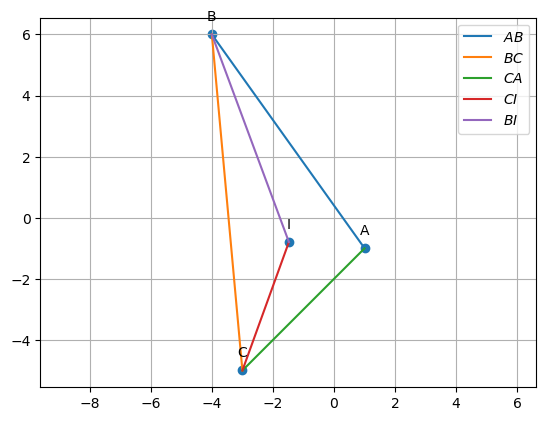
\includegraphics[width=\columnwidth]{solutions/1/5/2/figs/Incentre.png}
\caption{Intersection point $\vec{I}$ of angle bisectors of $\vec{B}$and$\vec{C}$ plotted using python}
\label{fig:i_tri_py}
\end{figure}



	\item Using 
    \eqref{eq:angle2d}
verify that 
		\begin{align}
			\angle BAI = \angle CAI.
		\end{align}
	\item Find the distance from $\vec{I}$ to $BC$.  \\
        \iffalse
\let\negmedspace\undefined
\let\negthickspace\undefined
\documentclass[journal,12pt,twocolumn]{IEEEtran}
\usepackage{cite}
\usepackage{amsmath,amssymb,amsfonts,amsthm}
\usepackage{algorithmic}
\usepackage{graphicx}
\usepackage{textcomp}
\usepackage{xcolor}
\usepackage{txfonts}
\usepackage{listings}
\usepackage{enumitem}
\usepackage{mathtools}
\usepackage{gensymb}
\usepackage[breaklinks=true]{hyperref}
\usepackage{tkz-euclide} % loads  TikZ and tkz-base
\usepackage{listings}
%\usepackage{gvv}

\newtheorem{theorem}{Theorem}[section]
\newtheorem{problem}{Problem}
\newtheorem{proposition}{Proposition}[section]
\newtheorem{lemma}{Lemma}[section]
\newtheorem{corollary}[theorem]{Corollary}
\newtheorem{example}{Example}[section]
\newtheorem{definition}[problem]{Definition}
\newcommand{\BEQA}{\begin{eqnarray}}
\newcommand{\EEQA}{\end{eqnarray}}
\newcommand{\define}{\stackrel{\triangle}{=}}
\theoremstyle{remark}
\newtheorem{rem}{Remark}

\begin{document}
\bibliographystyle{IEEEtran}
\vspace{3cm}
\title{
%	\logo{
Assignment
%	}
}
\author{ Antalene (EE22BTECH11008)}
\maketitle
\renewcommand{\thefigure}{\theenumi}
\renewcommand{\thetable}{\theenumi}

\providecommand{\pr}[1]{\ensuremath{\Pr\left(#1\right)}}
\providecommand{\prt}[2]{\ensuremath{p_{#1}^{\left(#2\right)} }}        % own macro for this question
\providecommand{\qfunc}[1]{\ensuremath{Q\left(#1\right)}}
\providecommand{\sbrak}[1]{\ensuremath{{}\left[#1\right]}}
\providecommand{\lsbrak}[1]{\ensuremath{{}\left[#1\right.}}
\providecommand{\rsbrak}[1]{\ensuremath{{}\left.#1\right]}}
\providecommand{\brak}[1]{\ensuremath{\left(#1\right)}}
\providecommand{\lbrak}[1]{\ensuremath{\left(#1\right.}}
\providecommand{\rbrak}[1]{\ensuremath{\left.#1\right)}}
\providecommand{\cbrak}[1]{\ensuremath{\left\{#1\right\}}}
\providecommand{\lcbrak}[1]{\ensuremath{\left\{#1\right.}}
\providecommand{\rcbrak}[1]{\ensuremath{\left.#1\right\}}}
\newcommand{\sgn}{\mathop{\mathrm{sgn}}}
\providecommand{\abs}[1]{\left\vert#1\right\vert}
\providecommand{\res}[1]{\Res\displaylimits_{#1}} 
\providecommand{\norm}[1]{\left\lVert#1\right\rVert}
%\providecommand{\norm}[1]{\lVert#1\rVert}
\providecommand{\mtx}[1]{\mathbf{#1}}
\providecommand{\mean}[1]{E\left[ #1 \right]}
\providecommand{\cond}[2]{#1\middle|#2}
\providecommand{\fourier}{\overset{\mathcal{F}}{ \rightleftharpoons}}
\newenvironment{amatrix}[1]{%
  \left(\begin{array}{@{}*{#1}{c}|c@{}}
}{%
  \end{array}\right)
}
%\providecommand{\hilbert}{\overset{\mathcal{H}}{ \rightleftharpoons}}
%\providecommand{\system}{\overset{\mathcal{H}}{ \longleftrightarrow}}
	%\newcommand{\solution}[2]{\textbf{Solution:}{#1}}
\newcommand{\solution}{\noindent \textbf{Solution: }}
\newcommand{\cosec}{\,\text{cosec}\,}
\providecommand{\dec}[2]{\ensuremath{\overset{#1}{\underset{#2}{\gtrless}}}}
\newcommand{\myvec}[1]{\ensuremath{\begin{pmatrix}#1\end{pmatrix}}}
\newcommand{\mydet}[1]{\enuremath{\begin{vmatrix}#1\end{vmatrix}}}
\newcommand{\myaugvec}[2]{\ensuremath{\begin{amatrix}{#1}#2\end{amatrix}}}
\providecommand{\rank}{\text{rank}}
\providecommand{\pr}[1]{\ensuremath{\Pr\left(#1\right)}}
\providecommand{\qfunc}[1]{\ensuremath{Q\left(#1\right)}}
	\newcommand*{\permcomb}[4][0mu]{{{}^{#3}\mkern#1#2_{#4}}}
\newcommand*{\perm}[1][-3mu]{\permcomb[#1]{P}}
\newcommand*{\comb}[1][-1mu]{\permcomb[#1]{C}}
\providecommand{\qfunc}[1]{\ensuremath{Q\left(#1\right)}}
\providecommand{\gauss}[2]{\mathcal{N}\ensuremath{\left(#1,#2\right)}}
\providecommand{\diff}[2]{\ensuremath{\frac{d{#1}}{d{#2}}}}
\providecommand{\myceil}[1]{\left \lceil #1 \right \rceil }
\newcommand\figref{Fig.~\ref}
\newcommand\tabref{Table~\ref}
\newcommand{\sinc}{\,\text{sinc}\,}
\newcommand{\rect}{\,\text{rect}\,}
%%
%	%\newcommand{\solution}[2]{\textbf{Solution:}{#1}}
%\newcommand{\solution}{\noindent \textbf{Solution: }}
%\newcommand{\cosec}{\,\text{cosec}\,}
%\numberwithin{equation}{section}
%\numberwithin{equation}{subsection}
%\numberwithin{problem}{section}
%\numberwithin{definition}{section}
%\makeatletter
%\@addtoreset{figure}{problem}
%\makeatother

%\let\StandardTheFigure\thefigure
\let\vec\mathbf



%my code starts from here
Question 1.5.4\\
Find the distance from $\vec{I}$ to $BC$.\\
\fi
\solution
\text{the value of $\vec{I}$ from ... is }\\ %refernence value will come here \eqref{ival}
\begin{align}
\vec{I} &= \frac{1}{\sqrt{37} + 4 + \sqrt{61}} \myvec{\sqrt{61} - 16 - 3\sqrt{37}\\ -\sqrt{61} + 24 - 5\sqrt{37}}\\
&=\myvec{-1.48\\ -0.79}\\
\end{align}
\text{Equation of $BC$ from ... is}\\%refernence value will come here \eqref{BC}
\begin{align}
BC: \myvec{11 & 1}\vec{x} =50\\
\end{align}
Then, the distance between point $\vec{I}$ and line $BC$ is
\begin{align}
&=\frac{\abs{\myvec{11&1} \vec{I} - 50}}{\norm{\myvec{11 \\ 1}}}\\
&=\frac{\abs{\myvec{11&1} \myvec{-1.48 \\ -0.79} - 50}}{\sqrt{122}}\\
&=\frac{\abs{-67.07}}{\sqrt{122}}\\
&=6.072
\end{align}


	\item Repeat the above exercise for the sides $AB$ and $AC$.
	\item This distance is known as the {\em inradius} $r$.
	\item Draw a circle with center $\vec{I}$ and radius $r$.  $\vec{I}$ is known as the {\em incentre}.
	\item The equation of the {\em incircle} is given by 
		\begin{align}
			\norm{\vec{x}-\vec{I}}^2 = r^2
		\end{align}
		Find the parameteric equation of $BC$ and use it to verify that $BC$ intersects the incircle at exactly one point $\vec{D}_3$.  $BC$ is defined to be a {\em tangent} to the incircle.  $\vec{D}_3$ is defined to be {\em point of contact}.
	\\
		%% Run LaTeX on this file several times to get Table of Contents,
%% cross-references, and citations.

\documentclass[11pt]{book}
\usepackage{gvv-book}
\usepackage{gvv}
%\usepackage{Wiley-AuthoringTemplate}
\usepackage[sectionbib,authoryear]{natbib}% for name-date citation comment the below line
%\usepackage[sectionbib,numbers]{natbib}% for numbered citation comment the above line

%%********************************************************************%%
%%       How many levels of section head would you like numbered?     %%
%% 0= no section numbers, 1= section, 2= section, 3= subsection %%
\setcounter{secnumdepth}{3}
%%********************************************************************%%
%%**********************************************************************%%
%%     How many levels of section head would you like to appear in the  %%
%%				Table of Contents?			%%
%% 0= chapter, 1= section, 2= section, 3= subsection titles.	%%
\setcounter{tocdepth}{2}
%%**********************************************************************%%

%\includeonly{ch01}
\makeindex

\begin{document}

\frontmatter
%%%%%%%%%%%%%%%%%%%%%%%%%%%%%%%%%%%%%%%%%%%%%%%%%%%%%%%%%%%%%%%%
%% Title Pages
%% Wiley will provide title and copyright page, but you can make
%% your own titlepages if you'd like anyway
%% Setting up title pages, type in the appropriate names here:

\booktitle{Geometry}

\subtitle{Through Algebra}

\AuAff{G. V. V. Sharma}


%% \\ will start a new line.
%% You may add \affil{} for affiliation, ie,
%\authors{Robert M. Groves\\
%\affil{Universitat de les Illes Balears}
%Floyd J. Fowler, Jr.\\
%\affil{University of New Mexico}
%}

%% Print Half Title and Title Page:
%\halftitlepage
\titlepage

%%%%%%%%%%%%%%%%%%%%%%%%%%%%%%%%%%%%%%%%%%%%%%%%%%%%%%%%%%%%%%%%
%% Copyright Page

\begin{copyrightpage}{2022}
%Title, etc
\end{copyrightpage}

% Note, you must use \ to start indented lines, ie,
% 
% \begin{copyrightpage}{2004}
% Survey Methodology / Robert M. Groves . . . [et al.].
% \       p. cm.---(Wiley series in survey methodology)
% \    ``Wiley-Interscience."
% \    Includes bibliographical references and index.
% \    ISBN 0-471-48348-6 (pbk.)
% \    1. Surveys---Methodology.  2. Social 
% \  sciences---Research---Statistical methods.  I. Groves, Robert M.  II. %
% Series.\\

% HA31.2.S873 2004
% 001.4'33---dc22                                             2004044064
% \end{copyrightpage}

%%%%%%%%%%%%%%%%%%%%%%%%%%%%%%%%%%%%%%%%%%%%%%%%%%%%%%%%%%%%%%%%
%% Only Dedication (optional) 

%\dedication{To my parents}

\tableofcontents

%\listoffigures %optional
%\listoftables  %optional

%% or Contributor Page for edited books
%% before \tableofcontents

%%%%%%%%%%%%%%%%%%%%%%%%%%%%%%%%%%%%%%%%%%%%%%%%%%%%%%%%%%%%%%%%
%  Contributors Page for Edited Book
%%%%%%%%%%%%%%%%%%%%%%%%%%%%%%%%%%%%%%%%%%%%%%%%%%%%%%%%%%%%%%%%

% If your book has chapters written by different authors,
% you'll need a Contributors page.

% Use \begin{contributors}...\end{contributors} and
% then enter each author with the \name{} command, followed
% by the affiliation information.

% \begin{contributors}
% \name{Masayki Abe,} Fujitsu Laboratories Ltd., Fujitsu Limited, Atsugi, Japan
%
% \name{L. A. Akers,} Center for Solid State Electronics Research, Arizona State University, Tempe, Arizona
%
% \name{G. H. Bernstein,} Department of Electrical and Computer Engineering, University of Notre Dame, Notre Dame, South Bend, Indiana; formerly of
% Center for Solid State Electronics Research, Arizona
% State University, Tempe, Arizona 
% \end{contributors}

%%%%%%%%%%%%%%%%%%%%%%%%%%%%%%%%%%%%%%%%%%%%%%%%%%%%%%%%%%%%%%%%
% Optional Foreword:

%\begin{foreword}
%\lipsum[1-2]
%\end{foreword}

%%%%%%%%%%%%%%%%%%%%%%%%%%%%%%%%%%%%%%%%%%%%%%%%%%%%%%%%%%%%%%%%
% Optional Preface:

%\begin{preface}
%\lipsum[1-1]
%\prefaceauthor{}
%\where{place\\
% date}
%\end{preface}

% ie,
% \begin{preface}
% This is an example preface.
% \prefaceauthor{R. K. Watts}
% \where{Durham, North Carolina\\
% September, 2004}

%%%%%%%%%%%%%%%%%%%%%%%%%%%%%%%%%%%%%%%%%%%%%%%%%%%%%%%%%%%%%%%%
% Optional Acknowledgments:

%\acknowledgments
%\lipsum[1-2]
%\authorinitials{I. R. S.}  

%%%%%%%%%%%%%%%%%%%%%%%%%%%%%%%%
%% Glossary Type of Environment:

% \begin{glossary}
% \term{<term>}{<description>}
% \end{glossary}

%%%%%%%%%%%%%%%%%%%%%%%%%%%%%%%%
%\begin{acronyms}
%\acro{ASTA}{Arrivals See Time Averages}
%\acro{BHCA}{Busy Hour Call Attempts}
%\acro{BR}{Bandwidth Reservation}
%\acro{b.u.}{bandwidth unit(s)}
%\acro{CAC}{Call / Connection Admission Control}
%\acro{CBP}{Call Blocking Probability(-ies)}
%\acro{CCS}{Centum Call Seconds}
%\acro{CDTM}{Connection Dependent Threshold Model}
%\acro{CS}{Complete Sharing}
%\acro{DiffServ}{Differentiated Services}
%\acro{EMLM}{Erlang Multirate Loss Model}
%\acro{erl}{The Erlang unit of traffic-load}
%\acro{FIFO}{First in - First out}
%\acro{GB}{Global balance}
%\acro{GoS}{Grade of Service}
%\acro{ICT}{Information and Communication Technology}
%\acro{IntServ}{Integrated Services}
%\acro{IP}{Internet Protocol}
%\acro{ITU-T}{International Telecommunication Unit -- Standardization sector}
%\acro{LB}{Local balance}
%\acro{LHS}{Left hand side}
%\acro{LIFO}{Last in - First out}
%\acro{MMPP}{Markov Modulated Poisson Process}
%\acro{MPLS}{Multiple Protocol Labeling Switching}
%\acro{MRM}{Multi-Retry Model}
%\acro{MTM}{Multi-Threshold Model}
%\acro{PASTA}{Poisson Arrivals See Time Averages}
%\acro{PDF}{Probability Distribution Function}
%\acro{pdf}{probability density function}
%\acro{PFS}{Product Form Solution}
%\acro{QoS}{Quality of Service}
%\acro{r.v.}{random variable(s)}
%\acro{RED}{random early detection}
%\acro{RHS}{Right hand side}
%\acro{RLA}{Reduced Load Approximation}
%\acro{SIRO}{service in random order}
%\acro{SRM}{Single-Retry Model}
%\acro{STM}{Single-Threshold Model}
%\acro{TCP}{Transport Control Protocol}
%\acro{TH}{Threshold(s)}
%\acro{UDP}{User Datagram Protocol}
%\end{acronyms}

\setcounter{page}{1}

\begin{introduction}
This book shows how to solve problems in geometry using trigonometry and coordinate geometry. 

\end{introduction}

\mainmatter

\chapter{Triangle}
Consider a triangle with vertices
		\begin{align}
			\label{eq:tri-pts}
			\vec{A} = \myvec{1 \\ -1},\,
			\vec{B} = \myvec{-4 \\ 6},\,
			\vec{C} = \myvec{-3 \\ -5}
		\end{align}
\section{Vectors}
%\renewcommand{\theequation}{\theenumi}
%\begin{enumerate}[label=\arabic*.,ref=\theenumi]
\begin{enumerate}[label=\thesection.\arabic*.,ref=\thesection.\theenumi]
\numberwithin{equation}{enumi}
\item The direction vector of $AB$ is defined as
		\begin{align}
			\vec{B}-
			\vec{A}
		\end{align}
Find the direction vectors of $AB, BC$ and $CA$.
\\
	\input{solutions/1/1/1/prob_1.tex}
	\item The length of side $BC$ is 
		\begin{align}
			\norm{\vec{B}-\vec{A}} \triangleq \sqrt{\brak{\vec{B}-\vec{A}}^{\top}{\vec{B}-\vec{A}}}
		\end{align}
		where
		\begin{align}
			\vec{A}^{\top}\triangleq\myvec{1 & -1}
		\end{align}
  \\		\input{solutions/1/1/2/main.tex}
\item   Points $\vec{A}, \vec{B}, \vec{C}$ are defined to be collinear if 
		\begin{align}
			\rank{\myvec{1 & 1 & 1 \\ \vec{A}& \vec{B}&\vec{C}}} = 2
		\end{align}
Are the given points in
			\eqref{eq:tri-pts}
collinear?\\
\input{solutions/1/1/3/main.tex}
\item The parameteric form of the equation  of $AB$ is 
		\begin{align}
			\vec{x}=\vec{A}+k\vec{m}
		\end{align}
		where
		\begin{align}
\vec{m}=\vec{B}-\vec{A}
		\end{align}
is the direction vector of $AB$.
Find the parameteric equations of $AB, BC$ and $CA$.
\\
		\input{solutions/1/1/4/main.tex}
\item The normal form of the equation of $AB$  is 
		\begin{align}
			\vec{n}^{\top}\brak{	\vec{x}-\vec{A}} = 0
		\end{align}
		where 
		\begin{align}
			\vec{n}^{\top}\vec{m}&=\vec{n}^{\top}\brak{\vec{B}-\vec{A}} = 0
			\\
			\text{or, } \vec{n}&=\myvec{0 & 1 \\ -1 & 0} \vec{m}
		\end{align}
Find the normal form of the equations of $AB, BC$ and $CA$.
\input{solutions/1/1/5/assign1.tex}
\input{solutions/1/1/5a/assignment1.tex}
\input{solutions/1/1/5c/main.tex}
\item The area of $\triangle ABC$ is defined as
		\begin{align}
			\frac{1}{2}\norm{{\brak{\vec{A}-\vec{B}}\times {\vec{A}-\vec{C}}}}
		\end{align}
		where
		\begin{align}
			\vec{A}\times\vec{B} \triangleq \mydet{1 & -4 \\-1 & 6}
		\end{align}
		Find the area of $\triangle ABC$.\\
  		\input{solutions/1/1/6/main.tex}
	\item Find the angles $A, B, C$ if 
    \label{prop:angle2d}
  \begin{align}
    \label{eq:angle2d}
			\cos A \triangleq 
\frac{\brak{\vec{B}-\vec{A}}^{\top}{\vec{C}-\vec{A}}}{\norm{\vec{B}-\vec{A}}\norm{\vec{C}-\vec{A}}}
  \end{align}\\
  	\input{solutions/1/1/7/main.tex}
\end{enumerate}

\section{Median}
%\renewcommand{\theequation}{\theenumi}
%\begin{enumerate}[label=\arabic*.,ref=\theenumi]
\begin{enumerate}[label=\thesection.\arabic*.,ref=\thesection.\theenumi]
\numberwithin{equation}{enumi}
\item If $\vec{D}$ divides $BC$ in the ratio $k : 1$,
		\begin{align}
			\vec{D}= \frac{k\vec{C}+\vec{B}}{k+1}
		\end{align}
		Find the mid points $\vec{D}, \vec{E}, \vec{F}$ of the sides $BC, CA$ and $AB$ respectively.
		\\
			\input{solutions/1/2/1/main.tex} 
	\item Find the equations of $AD, BE$ and $CF$.
	\item Find the intersection $\vec{G}$ of $BE$ and $CF$.
	\item Verify that 
		\begin{align}
			\frac{BG}{GE} = 
			\frac{CG}{GF} =
			\frac{AG}{GD} =2 
		\end{align}
	\item Show that $\vec{A}, \vec{G}$ and $\vec{D}$ are collinear.
	\item Verify that 
		\begin{align}
			\vec{G}=\frac{\vec{A}+\vec{B}+\vec{C}}{3}
		\end{align}
			$\vec{G}$ is known as the {\em centroid} of $\triangle ABC$.
   \\
		\input{solutions/1/2/6/main.tex}
	\item Verify that 
		\begin{align}
\vec{A}-\vec{F}=\vec{E}-\vec{D}
		\end{align}
		The quadrilateral $AFDE$ is defined to be a parallelogram.
\end{enumerate}

\section{Altitude}
%\renewcommand{\theequation}{\theenumi}
%\begin{enumerate}[label=\arabic*.,ref=\theenumi]
\begin{enumerate}[label=\thesection.\arabic*.,ref=\thesection.\theenumi]
\numberwithin{equation}{enumi}
\item $\vec{D}_1$ is a point on $BC$ such that
		\begin{align}
			AD_1 \perp BC
		\end{align}
		and $AD_1$ is defined to be the altitude. 
		Find the normal vector of $AD_1$.
  \\
		\input{solutions/1/3/1/main.tex}
	\item Find the equation of $AD_1$.

	\item Find the equations of the altitudes $BE_1$ and $CF_1$ to the sides $AC$ and $AB$ respectively. 
	\item Find the intersection $\vec{H}$ of $BE_1$ and $CF_1$.
	\item Verify that 
		\begin{align}
			\brak{\vec{A}-\vec{H}}^{\top}\brak{\vec{B}-\vec{C}} = 0
		\end{align}
  \\
  	\input{solutions/1/3/5/main.tex}
\end{enumerate}

\section{Perpendicular Bisector}
%\renewcommand{\theequation}{\theenumi}
%\begin{enumerate}[label=\arabic*.,ref=\theenumi]
\begin{enumerate}[label=\thesection.\arabic*.,ref=\thesection.\theenumi]
\numberwithin{equation}{enumi}

\item The equation of the perpendicular bisector of $BC$ is
		\begin{align}
			\label{eq:tri-perp-bisect}
			\brak{\vec{x}-\frac{\vec{B}+\vec{C}}{2}}\brak{\vec{B}-\vec{C}} = 0
		\end{align}
		Substitute numerical values and find the equations of the perpendicular bisectors of $AB, BC$ and $CA$.
	\\	\input{solutions/1/4/1/q1.4.1.tex}
	\item Find the intersection $\vec{O}$ of the perpendicular bisectors of $AB$ and $AC$.
 \\
 \input{solutions/1/4/2/main.tex}
	\item Verify that $\vec{O}$ satisfies
			\eqref{eq:tri-perp-bisect}.
$\vec{O}$ is known as the circumcentre.\\
   \input{solutions/1/4/3/main.tex}
		\item Verify that 
		\begin{align}
			OA = OB = OC 
		\end{align}
  \\
  \input{solutions/1/4/4/main.tex}
  \input{solutions/1/4/4(1)/main.tex}
	\item Draw the circle with centre at $\vec{O}$ and radius 
		\begin{align}
			R = OA
		\end{align}
		This is known as the {\em circumradius}. 
  \\  \input{solutions/1/4/5/assignment2.tex}
	\item Verify that 
		\begin{align}
			\angle BOC = 2\angle BAC.
		\end{align}\\
  \input{solutions/1/4/6/Q_1.4.6.tex}
	\item Let 
		\begin{align}
			\vec{P} = \myvec{\cos \theta & -\sin \theta \\ \sin \theta & \cos \theta}
		\end{align}
		Find $\theta$ if 
		\begin{align}
			\vec{C}-\vec{O}=\vec{P}\brak{\vec{A}-\vec{O}}
		\end{align}
\end{enumerate}

\section{Angle Bisector}
%\renewcommand{\theequation}{\theenumi}
%\begin{enumerate}[label=\arabic*.,ref=\theenumi]
\begin{enumerate}[label=\thesection.\arabic*.,ref=\thesection.\theenumi]
\numberwithin{equation}{enumi}
\item Suppose the equations $AB, BC$ and $CA$ are respectively given by 
		\begin{align}
			\label{eq:tri-sides}
			\vec{n}_i^{\top}\vec{x}=c_i \quad i = 1, 2, 3 
		\end{align}
		The equations of the respective angle bisectors are then given by 
		\begin{align}
			\frac{\vec{n}_i^{\top}\vec{x}-c_i}{\norm{\vec{n}_i}}
		=
	\pm	\frac{\vec{n}_j^{\top}\vec{x}-c_j}{\norm{\vec{n}_j}}
\quad i \ne j
		\end{align}
		Substitute numerical values and find the equations of the angle bisectors of $A, B$ and $C$.
	\\
		%\input{solutions/1/5/1/Assignment_1.tex}
  \input{solutions/1/5/1(1)/main.tex}
	\item Find the intersection $\vec{I}$ of the angle bisectors of $B$ and $C$.
 \\
		\input{solutions/1/5/2/main.tex}
	\item Using 
    \eqref{eq:angle2d}
verify that 
		\begin{align}
			\angle BAI = \angle CAI.
		\end{align}
	\item Find the distance from $\vec{I}$ to $BC$.  \\
        \input{solutions/1/5/4/main.tex}
	\item Repeat the above exercise for the sides $AB$ and $AC$.
	\item This distance is known as the {\em inradius} $r$.
	\item Draw a circle with center $\vec{I}$ and radius $r$.  $\vec{I}$ is known as the {\em incentre}.
	\item The equation of the {\em incircle} is given by 
		\begin{align}
			\norm{\vec{x}-\vec{I}}^2 = r^2
		\end{align}
		Find the parameteric equation of $BC$ and use it to verify that $BC$ intersects the incircle at exactly one point $\vec{D}_3$.  $BC$ is defined to be a {\em tangent} to the incircle.  $\vec{D}_3$ is defined to be {\em point of contact}.
	\\
		\input{solutions/1/5/8/main.tex}
  \item Find the other points of contact $\vec{E}_3$ and $\vec{F}_3$.
	\item Verify that 
		\begin{align}
			AE_3 = AF_3=m, BD_3 = BF_3=n, CD_3 = CE_3=p.
		\end{align}
	\item Obtain $m,n,p$ in terms of $a,b,c$, the sides of the triangle using a matrix equation.  Obtain the numerical values.
 \\
 		\input{solutions/1/5/11/main.tex}
\end{enumerate}

%
\chapter{Linear Equations}
\section{9}
\subsection{9.3.3}
\input{chapters/9/9.3.3.tex}
\subsection{9.4.1}
\begin{enumerate}[label=\arabic*.,ref=\theenumi]
\item The cost of a notebook is twice the cost of a pen.Write a linear
equation in two variables to represent this statement.
(Take the Cost of a notebook to be $x$ and that of a pen to be
$y$).
\item Express the following linear equation in the form $ax+by+c=0$
and indicate the values of $a,b$ and $c$ in each case:
%\begin{enumerate}
\begin{enumerate}[label=(\roman*),ref=\theenumi]
\item $2x+3y=9.3\overline{5}$
\item $x-\frac{y}{5}-10=10$
\item $-2x+3y=6$
\item $ x=3y$
\item $2x=-5y$
\item $3x+2=0$
\item $y-2=0$
\item $5=2x$
\end{enumerate}
\end{enumerate}

\subsection{9.4.2}
\input{chapters/9/9.4.2.tex}
\subsection{9.4.3}
\begin{enumerate}[label=\arabic*.,ref=\theenumi]
\item Draw the graph of each of the following linear equations in two variables:
\begin{enumerate}[label=(\roman*),ref=\theenumi]
\item $x+y=4$
\item $x-y=2$
\item $y=3x$
\item $3=2x+y$
\end{enumerate}
\item Give the equations of two lines passing through (2,14).How many more such lines are there and 
why?
\item If the point(3,4) lies on the graph of the equation $3y=ax+7$ find the value of a
\item The taxi fare in the city is as follows:for te first kilometre,the fare is \rupee~8 and for the 
subsquent distance is \rupee~5 per km.Taking the distance Covered as $x$ km and total fare as
\rupee~y.Write a linear equation for this information,and draw its graph.
\item From the choices given below,choose the equation whose graphs are given Fig 4.6 Fig 4.7
\\
For fig-4.6 
\begin{enumerate}[label=(\roman*)]
\item $y=x$
\item $x+y=0$
\item $y=2x$
\item $2+3y=7x$
\end{enumerate} 
For fig-4.7 
\begin{enumerate}[label=(\roman*)]
\item $y=x+2$
\item $y=x-2$
\item $y=-x+2$
\item $x+2y=6$
\end{enumerate}
\begin{figure}[ht]
\centering
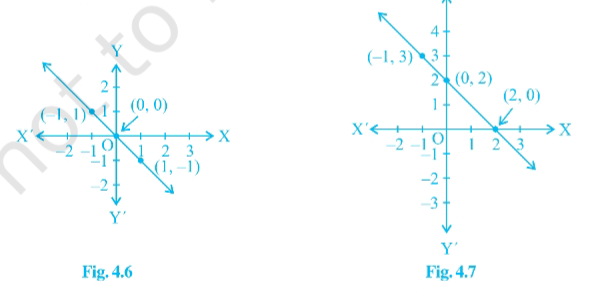
\includegraphics[width=\columnwidth]{chapters/9/figs/4.6-4.7.png}
\caption{Graph}
  \label{fig:4.6-4.7}
\end{figure}
\item If the work done by a body of a constant force is directly proportional 
to the distance travelled by the body,express this in the form of an equation
and draw the graph of the same by taking the varables and draw the graph of 
the same by taking the constant force as $5 units$.Also read from the graph the
work done when the distance travelled by the body is
\begin{enumerate}[label=(\roman*)]
\item $2$Units
\item $0$Unit
\end{enumerate}
\item Yamini and Fatima,two students of class IX of a school,together
 contributed \rupee~100 towards the prime minister's reief fund to help
 the earhquake victims.Write a linear equation which satisfies this data.
 (you may take their contributions  \rupee~x and \rupee~y.Draw the graph 
 of the same.
\item In Countries like USA and Canada temperature is measured in Celsius.
Here is a linear equation that converts Farenheit to celsius:
$F=\frac{9}{5}C+32$
\begin{enumerate}[label=(\roman*)]
\item Draw the graph of the linear equation above using Celsius for $x$
 axis and Farenheit for $y$ axis
\item If the temperature is $30\degree C$,what is the temperature in farenheight?
\item If the temperature is $95\degree F$,what is the temperature in celsius?
\item If the temperature is $0\degree C$.What is the temperature in Farenheit and if the temperature in celsius?
\item Is there a temperature Which is numerically same in both Farenheit and Celsius? If yes find it.
\end{enumerate}
\end{enumerate}

\section{10}
\subsection{Examples:-1-19 (10.3)}
\input{chapters/10/10.3.tex}
\subsection{10.3.1}
\input{chapters/10/10.3.1.tex}
\subsection{10.3.2}
\input{chapters/10/10.3.2.tex}
\subsection{10.3.3}
\begin{enumerate}
\item Solve the following pair of linear equations by the substitution method.
\begin{enumerate}[label=(\roman*)]    
	\item
	\begin{align}
   	 x+y=14 \\x-y=4
	\end{align}
    	\item 
	\begin{align}
	s-t=3
	\end{align}
	\item
	\begin{align}
    	3x-y=3\\ 9x-3y=9
	\end{align}
	\begin{align}   	
 	0.2x+0.3y=1.3\\ 0.4x+0.5y=23
	\end{align}
	\item     
	\begin{align}
	\sqrt{2x}+\sqrt{3y}=0\\ \sqrt{3x}-\sqrt{8y}=0
	\end{align}
	\item
	\begin{align}
    	\frac{3x}{2}-\frac{5y}{2}=-2\\ \frac{x}{3}+\frac{y}{2}=\frac{13}{6}
    	\end{align}
	\end{enumerate}
\item Solve $2x+3y=11$ and $2x+4y=-24$ and hence find the value of $m$ for which $y=mx+3$
\item Form the pair of linear equations for the following problems and find their solutions by the substitution method
    \begin{enumerate}[label=(\Roman*)]
    \item The difference between two numbers is $26$ and one number is three times the other. Find them.
    \item The larger of two supplementary angles exceeds the smaller by $18$ degrees. Find them.
    \item The coach of a cricket team buys $7$ balls and $6$ balls for \rupee~3800. Later, she buys $3$ bats and $5$ balls for \rupee~1750. Find the cost of each bat and each ball.
    \item The taxi charges in a city consist of a fixed charge together with the charges for the distance covered. For a distance of $10$ km, the charge paid is \rupee~105 and for a distance of $15$ km, the charge paid is \rupee~155. What are the fixed charges and the charge per km? How much does a person have to pay for travelling a distance of 25 km ? 
    \item A fraction becomes $\frac{9}{11}$ if $2$ is added to both the numerator and the denominator. If $3$ is added to both the numerator and the denominator, it becomes $\frac{5}{6}$. Find the fraction.
    \item Five years hence, the age of Jacob will be three times that of his son. Five years ago, Jacob's age was seven times that of his son. What are their present ages?
    \end{enumerate}
\end{enumerate}

\subsection{10.3.4}
\input{chapters/10/10.3.4.tex}
\subsection{10.3.5}
\input{chapters/10/10.3.5.tex}
\subsection{10.3.6}
\begin{enumerate}
\item Solve the following pair of equations by reducing them to a pair of linear equations:
\begin{enumerate}[label=(\roman*)]
\item
\begin{align}
\frac{1}{2x}+\frac{1}{3y}=2 \\ \frac{1}{3x}+\frac{1}{2y}=\frac{13}{6}
\end{align}
\item
\begin{align}
\frac{2}{\sqrt{x}}+\frac{3}{\sqrt{y}}=2\\
\frac{4}{\sqrt{x}}-\frac{9}{\sqrt{y}}=-1
\end{align}
\item
\begin{align}
\frac{4}{x}+3y=14\\ \frac{3}{x}-4y=23
\end{align}
\item
\begin{align}
\frac{5}{x-1}+\frac{1}{y-2}=2\\ \frac{6}{x-1}-\frac{3}{y-2}=1
\end{align}
\item
\begin{align}
\frac{7x-2y}{xy}=5\\ \frac{8x+7y}{xy}=15
\end{align}
\item
\begin{align}
6x+3y=6xy\\ 2x+4y=5xy
\end{align}
\item
\begin{align}
\frac{10}{x+y}+\frac{2}{x-y}=4\\ \frac{15}{x+y}-\frac{5}{x-y}=-2
\end{align}
\item
\begin{align}
\frac{1}{3x+y}+\frac{1}{3x-y}=\frac{3}{4}\\ \frac{1}{2(3x+y)}-\frac{1}{2(3x-y)}=\frac{-1}{8}
\end{align}
\end{enumerate}
\item Formulate the following problems as a pair of equations,and hence find their solutions:
\begin{enumerate}[label=(\roman*)]
\item Ritu can row downstream $20km$ in $2$ hours, and upstream $4km$ in $2$ hours. Find her speed of rowing in still water and the speed of the current.
\item $2$ women and $5$ men can together finish an embroidery work in $4$ days, while $3$ women and $6$ men can finish it in $3$ days. Find the time taken by $1$ women along to finish the work, and also that taken by $1$ men alone.
\item Roohi travels $300 km$ to her home partly by train and partly by bus. She takes $4$ hours if she travels $60km$ by train and the remaining by bus. If she travels $100km$ by train and the remaining by bus, she takes $10$ minutes longer. Find the speed of the train and the bus seperately.
\end{enumerate}
\end{enumerate}

\subsection{10.3.7}
\input{chapters/10/10.3.7.tex}
\chapter{Quadratic Equations}
\section{10}
\subsection{Examples:-1-18 (10.4)}                                               
\input{chapters/10/10.4.tex}
\subsection{10.4.1}
\input{chapters/10/10.4.1.tex}
\subsection{10.4.2}
\input{chapters/10/10.4.2.tex}
\subsection{10.4.3}
\input{chapters/10/10.4.3.tex}
\subsection{10.4.4}
\begin{enumerate}
\item Find the nature of the roots of the following quadratic equations. If real roots exist, find them:
\begin{enumerate}[label=(\roman*)]
\item $2x^2-3x+5=0$
\item $3x^2-4 sqrt 3x+4=0$
\item $2x^2-6x+3=0$
\end{enumerate}
\item Find the values of k for each of the following quadratic equations, so that they hav equal roots:
\begin{enumerate}[label=(\roman*)]
\item $2x^2=kx-3=0$
\item $kx(x-2)+6=0$
\end{enumerate}
\item Is it possible to design a rectangular mango grove whose length is twice its breadth, and the area is  $800m^2$? If so, find its length and breadth.
\item Is the following situation possible? If so, determine their present ages.
\\ The sum of the ages of the two friends is 20 years. Four years ago, the product of their ages in years was $48$.
\item Is it possible to design a rectangular park of perimeter 80m and area of $400m^2$. If so, find its length and breadth.
\end{enumerate}



\chapter{Coordinate Geometry}
\section{10}
\subsection{10.7.1}
\input{chapters/10/10.7.1.tex}
\subsection{10.7.2}
\input{chapters/10/10.7.2.tex}
\subsection{10.7.3}
\input{chapters/10/10.7.3.tex}
\subsection{10.7.4}
\input{chapters/10/10.7.4.tex}
\chapter{Straight Lines}
\section{11}
\subsection{11.10.1}
\input{chapters/11/11.10.1.tex}
\subsection{11.10.2}
\input{chapters/11/11.10.2.tex}
\subsection{11.10.3}
\input{chapters/11/11.10.3.tex}
\chapter{Trigonometry}
\section{Ratios}
\input{./chapters/trig/tri_geo_rt}
\section{The Baudhayana Theorem}
\input{./chapters/trig/tri_geo_baudh}
%
\section{Area of a Triangle}
\input{./chapters/trig/tri_geo_sincos}
\section{Angle Bisectors}
\input{./chapters/trig/ang.tex}
\section{Circumradius}
\input{./chapters/trig/tri_geo_cradius}
\section{Tangent}
\input{./chapters/trig/tangent}
\section{Identities}
\input{./chapters/trig/trig_id.tex}
\chapter{Analytic Geometry}
\section{Vectors}
\input{./chapters/coord/vector}
\section{Altitudes of a Triangle:Line Equation}
\input{./chapters/coord/tri_geo_alt}
\section{Circumcircle: Circle Equation}
\input{./chapters/coord/tri_geo_ccentre}
\section{Tangent}
\input{./chapters/coord/circ_geo_prop}
\chapter{Triangle}
\input{./chapters/exercises/tri_geo_exer}
\chapter{Quadrilateral}
\input{./chapters/exercises/quad_geo_exer}
%
\chapter{Circle}
\section{11}
\subsection{11.11.1}
In each of the following exercise \ref{prob:1} to \ref{prob:5}, find the equation of the circle with:
\begin{enumerate}[label=\arabic*.,ref=\thesubsection.\theenumi]
\item centre $(0,2)$ and radius $2$ \label{prob:1}
\item centre $(-2,3)$ and radius $4$
\item centre $\frac({1}{2},\frac{1}{4})$ and radius $\frac {1}{!2}$
\item centre $(1,1)$ and radius $2$
\item centre $(-a,-b)$ and radius $\sqrt{a^2-b^2}$  \label{prob:5}
\end{enumerate}
In each of the following exercise \ref{prob:6} to \ref{prob:9}, find the centre and radius of the circles
\begin{enumerate}[resume]
\item $(x-5)^2+(y-3)^2=36$ \label{prob:6}
\item $x^2+y^2-4x-8y-45=0$
\item $x^2+y^2-8x+10y-12=0$
\item $2x^2+2y^2-x=0$ \label{prob:9}
\end{enumerate}
\begin{enumerate}[resume]
\item Find the equation of the circle passing through the points $(4,1)$ and $(6,5)$ and whose centre is on the line $4x+y=16$.
\item Find the equation of the circle passing through the points $(2,3)$ and $(-1,1)$ and whose centre is on the line $x-3y-11=0$.
\item Find the equation of the circle with radius 5 whose centre lies on x-axis and passes through the point $(2,3)$.
\item Find the equation of the circle passing through $(0,0)$ and making intercepts $a$ and $b$ on the coordinate axes.
\item Find the equation of a circle with centre $(2,2)$ and passes through the point $(4,5)$.
\item Does the point $(-2.5,3.5)$ lie inside, outside or on the circle $x^2+y^2=25$.
\end{enumerate}



\input{./chapters/exercises/circ_geo_exer}
\chapter{Miscellaneous }
\input{./chapters/exercises/geo_misc}
\iffalse
%\include{ch02} 
\backmatter
\appendix
\chapter{Area of a Circle}
\input{./chapters/area/circ_geo_area}
\fi
%
%\chapter{Proofs}
%   \section{}
%\input{apps/defs.tex}

%  \section{}
%\input{apps/parab.tex}
%  \section{}
%\input{apps/nonparab.tex}
%		\section{}
%\input{apps/params.tex}
\latexprintindex

\end{document}

 

  \item Find the other points of contact $\vec{E}_3$ and $\vec{F}_3$.
	\item Verify that 
		\begin{align}
			AE_3 = AF_3=m, BD_3 = BF_3=n, CD_3 = CE_3=p.
		\end{align}
	\item Obtain $m,n,p$ in terms of $a,b,c$, the sides of the triangle using a matrix equation.  Obtain the numerical values.
 \\
 		%% Run LaTeX on this file several times to get Table of Contents,
%% cross-references, and citations.

\documentclass[11pt]{book}
\usepackage{gvv-book}
\usepackage{gvv}
%\usepackage{Wiley-AuthoringTemplate}
\usepackage[sectionbib,authoryear]{natbib}% for name-date citation comment the below line
%\usepackage[sectionbib,numbers]{natbib}% for numbered citation comment the above line

%%********************************************************************%%
%%       How many levels of section head would you like numbered?     %%
%% 0= no section numbers, 1= section, 2= section, 3= subsection %%
\setcounter{secnumdepth}{3}
%%********************************************************************%%
%%**********************************************************************%%
%%     How many levels of section head would you like to appear in the  %%
%%				Table of Contents?			%%
%% 0= chapter, 1= section, 2= section, 3= subsection titles.	%%
\setcounter{tocdepth}{2}
%%**********************************************************************%%

%\includeonly{ch01}
\makeindex

\begin{document}

\frontmatter
%%%%%%%%%%%%%%%%%%%%%%%%%%%%%%%%%%%%%%%%%%%%%%%%%%%%%%%%%%%%%%%%
%% Title Pages
%% Wiley will provide title and copyright page, but you can make
%% your own titlepages if you'd like anyway
%% Setting up title pages, type in the appropriate names here:

\booktitle{Geometry}

\subtitle{Through Algebra}

\AuAff{G. V. V. Sharma}


%% \\ will start a new line.
%% You may add \affil{} for affiliation, ie,
%\authors{Robert M. Groves\\
%\affil{Universitat de les Illes Balears}
%Floyd J. Fowler, Jr.\\
%\affil{University of New Mexico}
%}

%% Print Half Title and Title Page:
%\halftitlepage
\titlepage

%%%%%%%%%%%%%%%%%%%%%%%%%%%%%%%%%%%%%%%%%%%%%%%%%%%%%%%%%%%%%%%%
%% Copyright Page

\begin{copyrightpage}{2022}
%Title, etc
\end{copyrightpage}

% Note, you must use \ to start indented lines, ie,
% 
% \begin{copyrightpage}{2004}
% Survey Methodology / Robert M. Groves . . . [et al.].
% \       p. cm.---(Wiley series in survey methodology)
% \    ``Wiley-Interscience."
% \    Includes bibliographical references and index.
% \    ISBN 0-471-48348-6 (pbk.)
% \    1. Surveys---Methodology.  2. Social 
% \  sciences---Research---Statistical methods.  I. Groves, Robert M.  II. %
% Series.\\

% HA31.2.S873 2004
% 001.4'33---dc22                                             2004044064
% \end{copyrightpage}

%%%%%%%%%%%%%%%%%%%%%%%%%%%%%%%%%%%%%%%%%%%%%%%%%%%%%%%%%%%%%%%%
%% Only Dedication (optional) 

%\dedication{To my parents}

\tableofcontents

%\listoffigures %optional
%\listoftables  %optional

%% or Contributor Page for edited books
%% before \tableofcontents

%%%%%%%%%%%%%%%%%%%%%%%%%%%%%%%%%%%%%%%%%%%%%%%%%%%%%%%%%%%%%%%%
%  Contributors Page for Edited Book
%%%%%%%%%%%%%%%%%%%%%%%%%%%%%%%%%%%%%%%%%%%%%%%%%%%%%%%%%%%%%%%%

% If your book has chapters written by different authors,
% you'll need a Contributors page.

% Use \begin{contributors}...\end{contributors} and
% then enter each author with the \name{} command, followed
% by the affiliation information.

% \begin{contributors}
% \name{Masayki Abe,} Fujitsu Laboratories Ltd., Fujitsu Limited, Atsugi, Japan
%
% \name{L. A. Akers,} Center for Solid State Electronics Research, Arizona State University, Tempe, Arizona
%
% \name{G. H. Bernstein,} Department of Electrical and Computer Engineering, University of Notre Dame, Notre Dame, South Bend, Indiana; formerly of
% Center for Solid State Electronics Research, Arizona
% State University, Tempe, Arizona 
% \end{contributors}

%%%%%%%%%%%%%%%%%%%%%%%%%%%%%%%%%%%%%%%%%%%%%%%%%%%%%%%%%%%%%%%%
% Optional Foreword:

%\begin{foreword}
%\lipsum[1-2]
%\end{foreword}

%%%%%%%%%%%%%%%%%%%%%%%%%%%%%%%%%%%%%%%%%%%%%%%%%%%%%%%%%%%%%%%%
% Optional Preface:

%\begin{preface}
%\lipsum[1-1]
%\prefaceauthor{}
%\where{place\\
% date}
%\end{preface}

% ie,
% \begin{preface}
% This is an example preface.
% \prefaceauthor{R. K. Watts}
% \where{Durham, North Carolina\\
% September, 2004}

%%%%%%%%%%%%%%%%%%%%%%%%%%%%%%%%%%%%%%%%%%%%%%%%%%%%%%%%%%%%%%%%
% Optional Acknowledgments:

%\acknowledgments
%\lipsum[1-2]
%\authorinitials{I. R. S.}  

%%%%%%%%%%%%%%%%%%%%%%%%%%%%%%%%
%% Glossary Type of Environment:

% \begin{glossary}
% \term{<term>}{<description>}
% \end{glossary}

%%%%%%%%%%%%%%%%%%%%%%%%%%%%%%%%
%\begin{acronyms}
%\acro{ASTA}{Arrivals See Time Averages}
%\acro{BHCA}{Busy Hour Call Attempts}
%\acro{BR}{Bandwidth Reservation}
%\acro{b.u.}{bandwidth unit(s)}
%\acro{CAC}{Call / Connection Admission Control}
%\acro{CBP}{Call Blocking Probability(-ies)}
%\acro{CCS}{Centum Call Seconds}
%\acro{CDTM}{Connection Dependent Threshold Model}
%\acro{CS}{Complete Sharing}
%\acro{DiffServ}{Differentiated Services}
%\acro{EMLM}{Erlang Multirate Loss Model}
%\acro{erl}{The Erlang unit of traffic-load}
%\acro{FIFO}{First in - First out}
%\acro{GB}{Global balance}
%\acro{GoS}{Grade of Service}
%\acro{ICT}{Information and Communication Technology}
%\acro{IntServ}{Integrated Services}
%\acro{IP}{Internet Protocol}
%\acro{ITU-T}{International Telecommunication Unit -- Standardization sector}
%\acro{LB}{Local balance}
%\acro{LHS}{Left hand side}
%\acro{LIFO}{Last in - First out}
%\acro{MMPP}{Markov Modulated Poisson Process}
%\acro{MPLS}{Multiple Protocol Labeling Switching}
%\acro{MRM}{Multi-Retry Model}
%\acro{MTM}{Multi-Threshold Model}
%\acro{PASTA}{Poisson Arrivals See Time Averages}
%\acro{PDF}{Probability Distribution Function}
%\acro{pdf}{probability density function}
%\acro{PFS}{Product Form Solution}
%\acro{QoS}{Quality of Service}
%\acro{r.v.}{random variable(s)}
%\acro{RED}{random early detection}
%\acro{RHS}{Right hand side}
%\acro{RLA}{Reduced Load Approximation}
%\acro{SIRO}{service in random order}
%\acro{SRM}{Single-Retry Model}
%\acro{STM}{Single-Threshold Model}
%\acro{TCP}{Transport Control Protocol}
%\acro{TH}{Threshold(s)}
%\acro{UDP}{User Datagram Protocol}
%\end{acronyms}

\setcounter{page}{1}

\begin{introduction}
This book shows how to solve problems in geometry using trigonometry and coordinate geometry. 

\end{introduction}

\mainmatter

\chapter{Triangle}
Consider a triangle with vertices
		\begin{align}
			\label{eq:tri-pts}
			\vec{A} = \myvec{1 \\ -1},\,
			\vec{B} = \myvec{-4 \\ 6},\,
			\vec{C} = \myvec{-3 \\ -5}
		\end{align}
\section{Vectors}
%\renewcommand{\theequation}{\theenumi}
%\begin{enumerate}[label=\arabic*.,ref=\theenumi]
\begin{enumerate}[label=\thesection.\arabic*.,ref=\thesection.\theenumi]
\numberwithin{equation}{enumi}
\item The direction vector of $AB$ is defined as
		\begin{align}
			\vec{B}-
			\vec{A}
		\end{align}
Find the direction vectors of $AB, BC$ and $CA$.
\\
	\input{solutions/1/1/1/prob_1.tex}
	\item The length of side $BC$ is 
		\begin{align}
			\norm{\vec{B}-\vec{A}} \triangleq \sqrt{\brak{\vec{B}-\vec{A}}^{\top}{\vec{B}-\vec{A}}}
		\end{align}
		where
		\begin{align}
			\vec{A}^{\top}\triangleq\myvec{1 & -1}
		\end{align}
  \\		\input{solutions/1/1/2/main.tex}
\item   Points $\vec{A}, \vec{B}, \vec{C}$ are defined to be collinear if 
		\begin{align}
			\rank{\myvec{1 & 1 & 1 \\ \vec{A}& \vec{B}&\vec{C}}} = 2
		\end{align}
Are the given points in
			\eqref{eq:tri-pts}
collinear?\\
\input{solutions/1/1/3/main.tex}
\item The parameteric form of the equation  of $AB$ is 
		\begin{align}
			\vec{x}=\vec{A}+k\vec{m}
		\end{align}
		where
		\begin{align}
\vec{m}=\vec{B}-\vec{A}
		\end{align}
is the direction vector of $AB$.
Find the parameteric equations of $AB, BC$ and $CA$.
\\
		\input{solutions/1/1/4/main.tex}
\item The normal form of the equation of $AB$  is 
		\begin{align}
			\vec{n}^{\top}\brak{	\vec{x}-\vec{A}} = 0
		\end{align}
		where 
		\begin{align}
			\vec{n}^{\top}\vec{m}&=\vec{n}^{\top}\brak{\vec{B}-\vec{A}} = 0
			\\
			\text{or, } \vec{n}&=\myvec{0 & 1 \\ -1 & 0} \vec{m}
		\end{align}
Find the normal form of the equations of $AB, BC$ and $CA$.
\input{solutions/1/1/5/assign1.tex}
\input{solutions/1/1/5a/assignment1.tex}
\input{solutions/1/1/5c/main.tex}
\item The area of $\triangle ABC$ is defined as
		\begin{align}
			\frac{1}{2}\norm{{\brak{\vec{A}-\vec{B}}\times {\vec{A}-\vec{C}}}}
		\end{align}
		where
		\begin{align}
			\vec{A}\times\vec{B} \triangleq \mydet{1 & -4 \\-1 & 6}
		\end{align}
		Find the area of $\triangle ABC$.\\
  		\input{solutions/1/1/6/main.tex}
	\item Find the angles $A, B, C$ if 
    \label{prop:angle2d}
  \begin{align}
    \label{eq:angle2d}
			\cos A \triangleq 
\frac{\brak{\vec{B}-\vec{A}}^{\top}{\vec{C}-\vec{A}}}{\norm{\vec{B}-\vec{A}}\norm{\vec{C}-\vec{A}}}
  \end{align}\\
  	\input{solutions/1/1/7/main.tex}
\end{enumerate}

\section{Median}
%\renewcommand{\theequation}{\theenumi}
%\begin{enumerate}[label=\arabic*.,ref=\theenumi]
\begin{enumerate}[label=\thesection.\arabic*.,ref=\thesection.\theenumi]
\numberwithin{equation}{enumi}
\item If $\vec{D}$ divides $BC$ in the ratio $k : 1$,
		\begin{align}
			\vec{D}= \frac{k\vec{C}+\vec{B}}{k+1}
		\end{align}
		Find the mid points $\vec{D}, \vec{E}, \vec{F}$ of the sides $BC, CA$ and $AB$ respectively.
		\\
			\input{solutions/1/2/1/main.tex} 
	\item Find the equations of $AD, BE$ and $CF$.
	\item Find the intersection $\vec{G}$ of $BE$ and $CF$.
	\item Verify that 
		\begin{align}
			\frac{BG}{GE} = 
			\frac{CG}{GF} =
			\frac{AG}{GD} =2 
		\end{align}
	\item Show that $\vec{A}, \vec{G}$ and $\vec{D}$ are collinear.
	\item Verify that 
		\begin{align}
			\vec{G}=\frac{\vec{A}+\vec{B}+\vec{C}}{3}
		\end{align}
			$\vec{G}$ is known as the {\em centroid} of $\triangle ABC$.
   \\
		\input{solutions/1/2/6/main.tex}
	\item Verify that 
		\begin{align}
\vec{A}-\vec{F}=\vec{E}-\vec{D}
		\end{align}
		The quadrilateral $AFDE$ is defined to be a parallelogram.
\end{enumerate}

\section{Altitude}
%\renewcommand{\theequation}{\theenumi}
%\begin{enumerate}[label=\arabic*.,ref=\theenumi]
\begin{enumerate}[label=\thesection.\arabic*.,ref=\thesection.\theenumi]
\numberwithin{equation}{enumi}
\item $\vec{D}_1$ is a point on $BC$ such that
		\begin{align}
			AD_1 \perp BC
		\end{align}
		and $AD_1$ is defined to be the altitude. 
		Find the normal vector of $AD_1$.
  \\
		\input{solutions/1/3/1/main.tex}
	\item Find the equation of $AD_1$.

	\item Find the equations of the altitudes $BE_1$ and $CF_1$ to the sides $AC$ and $AB$ respectively. 
	\item Find the intersection $\vec{H}$ of $BE_1$ and $CF_1$.
	\item Verify that 
		\begin{align}
			\brak{\vec{A}-\vec{H}}^{\top}\brak{\vec{B}-\vec{C}} = 0
		\end{align}
  \\
  	\input{solutions/1/3/5/main.tex}
\end{enumerate}

\section{Perpendicular Bisector}
%\renewcommand{\theequation}{\theenumi}
%\begin{enumerate}[label=\arabic*.,ref=\theenumi]
\begin{enumerate}[label=\thesection.\arabic*.,ref=\thesection.\theenumi]
\numberwithin{equation}{enumi}

\item The equation of the perpendicular bisector of $BC$ is
		\begin{align}
			\label{eq:tri-perp-bisect}
			\brak{\vec{x}-\frac{\vec{B}+\vec{C}}{2}}\brak{\vec{B}-\vec{C}} = 0
		\end{align}
		Substitute numerical values and find the equations of the perpendicular bisectors of $AB, BC$ and $CA$.
	\\	\input{solutions/1/4/1/q1.4.1.tex}
	\item Find the intersection $\vec{O}$ of the perpendicular bisectors of $AB$ and $AC$.
 \\
 \input{solutions/1/4/2/main.tex}
	\item Verify that $\vec{O}$ satisfies
			\eqref{eq:tri-perp-bisect}.
$\vec{O}$ is known as the circumcentre.\\
   \input{solutions/1/4/3/main.tex}
		\item Verify that 
		\begin{align}
			OA = OB = OC 
		\end{align}
  \\
  \input{solutions/1/4/4/main.tex}
  \input{solutions/1/4/4(1)/main.tex}
	\item Draw the circle with centre at $\vec{O}$ and radius 
		\begin{align}
			R = OA
		\end{align}
		This is known as the {\em circumradius}. 
  \\  \input{solutions/1/4/5/assignment2.tex}
	\item Verify that 
		\begin{align}
			\angle BOC = 2\angle BAC.
		\end{align}\\
  \input{solutions/1/4/6/Q_1.4.6.tex}
	\item Let 
		\begin{align}
			\vec{P} = \myvec{\cos \theta & -\sin \theta \\ \sin \theta & \cos \theta}
		\end{align}
		Find $\theta$ if 
		\begin{align}
			\vec{C}-\vec{O}=\vec{P}\brak{\vec{A}-\vec{O}}
		\end{align}
\end{enumerate}

\section{Angle Bisector}
%\renewcommand{\theequation}{\theenumi}
%\begin{enumerate}[label=\arabic*.,ref=\theenumi]
\begin{enumerate}[label=\thesection.\arabic*.,ref=\thesection.\theenumi]
\numberwithin{equation}{enumi}
\item Suppose the equations $AB, BC$ and $CA$ are respectively given by 
		\begin{align}
			\label{eq:tri-sides}
			\vec{n}_i^{\top}\vec{x}=c_i \quad i = 1, 2, 3 
		\end{align}
		The equations of the respective angle bisectors are then given by 
		\begin{align}
			\frac{\vec{n}_i^{\top}\vec{x}-c_i}{\norm{\vec{n}_i}}
		=
	\pm	\frac{\vec{n}_j^{\top}\vec{x}-c_j}{\norm{\vec{n}_j}}
\quad i \ne j
		\end{align}
		Substitute numerical values and find the equations of the angle bisectors of $A, B$ and $C$.
	\\
		%\input{solutions/1/5/1/Assignment_1.tex}
  \input{solutions/1/5/1(1)/main.tex}
	\item Find the intersection $\vec{I}$ of the angle bisectors of $B$ and $C$.
 \\
		\input{solutions/1/5/2/main.tex}
	\item Using 
    \eqref{eq:angle2d}
verify that 
		\begin{align}
			\angle BAI = \angle CAI.
		\end{align}
	\item Find the distance from $\vec{I}$ to $BC$.  \\
        \input{solutions/1/5/4/main.tex}
	\item Repeat the above exercise for the sides $AB$ and $AC$.
	\item This distance is known as the {\em inradius} $r$.
	\item Draw a circle with center $\vec{I}$ and radius $r$.  $\vec{I}$ is known as the {\em incentre}.
	\item The equation of the {\em incircle} is given by 
		\begin{align}
			\norm{\vec{x}-\vec{I}}^2 = r^2
		\end{align}
		Find the parameteric equation of $BC$ and use it to verify that $BC$ intersects the incircle at exactly one point $\vec{D}_3$.  $BC$ is defined to be a {\em tangent} to the incircle.  $\vec{D}_3$ is defined to be {\em point of contact}.
	\\
		\input{solutions/1/5/8/main.tex}
  \item Find the other points of contact $\vec{E}_3$ and $\vec{F}_3$.
	\item Verify that 
		\begin{align}
			AE_3 = AF_3=m, BD_3 = BF_3=n, CD_3 = CE_3=p.
		\end{align}
	\item Obtain $m,n,p$ in terms of $a,b,c$, the sides of the triangle using a matrix equation.  Obtain the numerical values.
 \\
 		\input{solutions/1/5/11/main.tex}
\end{enumerate}

%
\chapter{Linear Equations}
\section{9}
\subsection{9.3.3}
\input{chapters/9/9.3.3.tex}
\subsection{9.4.1}
\begin{enumerate}[label=\arabic*.,ref=\theenumi]
\item The cost of a notebook is twice the cost of a pen.Write a linear
equation in two variables to represent this statement.
(Take the Cost of a notebook to be $x$ and that of a pen to be
$y$).
\item Express the following linear equation in the form $ax+by+c=0$
and indicate the values of $a,b$ and $c$ in each case:
%\begin{enumerate}
\begin{enumerate}[label=(\roman*),ref=\theenumi]
\item $2x+3y=9.3\overline{5}$
\item $x-\frac{y}{5}-10=10$
\item $-2x+3y=6$
\item $ x=3y$
\item $2x=-5y$
\item $3x+2=0$
\item $y-2=0$
\item $5=2x$
\end{enumerate}
\end{enumerate}

\subsection{9.4.2}
\input{chapters/9/9.4.2.tex}
\subsection{9.4.3}
\begin{enumerate}[label=\arabic*.,ref=\theenumi]
\item Draw the graph of each of the following linear equations in two variables:
\begin{enumerate}[label=(\roman*),ref=\theenumi]
\item $x+y=4$
\item $x-y=2$
\item $y=3x$
\item $3=2x+y$
\end{enumerate}
\item Give the equations of two lines passing through (2,14).How many more such lines are there and 
why?
\item If the point(3,4) lies on the graph of the equation $3y=ax+7$ find the value of a
\item The taxi fare in the city is as follows:for te first kilometre,the fare is \rupee~8 and for the 
subsquent distance is \rupee~5 per km.Taking the distance Covered as $x$ km and total fare as
\rupee~y.Write a linear equation for this information,and draw its graph.
\item From the choices given below,choose the equation whose graphs are given Fig 4.6 Fig 4.7
\\
For fig-4.6 
\begin{enumerate}[label=(\roman*)]
\item $y=x$
\item $x+y=0$
\item $y=2x$
\item $2+3y=7x$
\end{enumerate} 
For fig-4.7 
\begin{enumerate}[label=(\roman*)]
\item $y=x+2$
\item $y=x-2$
\item $y=-x+2$
\item $x+2y=6$
\end{enumerate}
\begin{figure}[ht]
\centering
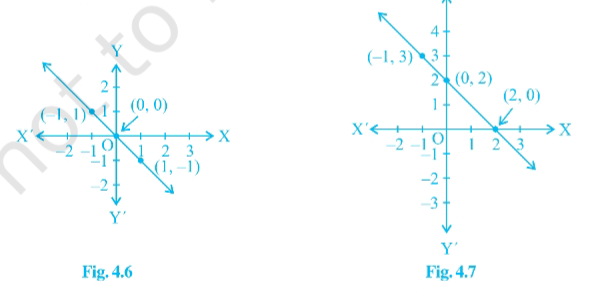
\includegraphics[width=\columnwidth]{chapters/9/figs/4.6-4.7.png}
\caption{Graph}
  \label{fig:4.6-4.7}
\end{figure}
\item If the work done by a body of a constant force is directly proportional 
to the distance travelled by the body,express this in the form of an equation
and draw the graph of the same by taking the varables and draw the graph of 
the same by taking the constant force as $5 units$.Also read from the graph the
work done when the distance travelled by the body is
\begin{enumerate}[label=(\roman*)]
\item $2$Units
\item $0$Unit
\end{enumerate}
\item Yamini and Fatima,two students of class IX of a school,together
 contributed \rupee~100 towards the prime minister's reief fund to help
 the earhquake victims.Write a linear equation which satisfies this data.
 (you may take their contributions  \rupee~x and \rupee~y.Draw the graph 
 of the same.
\item In Countries like USA and Canada temperature is measured in Celsius.
Here is a linear equation that converts Farenheit to celsius:
$F=\frac{9}{5}C+32$
\begin{enumerate}[label=(\roman*)]
\item Draw the graph of the linear equation above using Celsius for $x$
 axis and Farenheit for $y$ axis
\item If the temperature is $30\degree C$,what is the temperature in farenheight?
\item If the temperature is $95\degree F$,what is the temperature in celsius?
\item If the temperature is $0\degree C$.What is the temperature in Farenheit and if the temperature in celsius?
\item Is there a temperature Which is numerically same in both Farenheit and Celsius? If yes find it.
\end{enumerate}
\end{enumerate}

\section{10}
\subsection{Examples:-1-19 (10.3)}
\input{chapters/10/10.3.tex}
\subsection{10.3.1}
\input{chapters/10/10.3.1.tex}
\subsection{10.3.2}
\input{chapters/10/10.3.2.tex}
\subsection{10.3.3}
\begin{enumerate}
\item Solve the following pair of linear equations by the substitution method.
\begin{enumerate}[label=(\roman*)]    
	\item
	\begin{align}
   	 x+y=14 \\x-y=4
	\end{align}
    	\item 
	\begin{align}
	s-t=3
	\end{align}
	\item
	\begin{align}
    	3x-y=3\\ 9x-3y=9
	\end{align}
	\begin{align}   	
 	0.2x+0.3y=1.3\\ 0.4x+0.5y=23
	\end{align}
	\item     
	\begin{align}
	\sqrt{2x}+\sqrt{3y}=0\\ \sqrt{3x}-\sqrt{8y}=0
	\end{align}
	\item
	\begin{align}
    	\frac{3x}{2}-\frac{5y}{2}=-2\\ \frac{x}{3}+\frac{y}{2}=\frac{13}{6}
    	\end{align}
	\end{enumerate}
\item Solve $2x+3y=11$ and $2x+4y=-24$ and hence find the value of $m$ for which $y=mx+3$
\item Form the pair of linear equations for the following problems and find their solutions by the substitution method
    \begin{enumerate}[label=(\Roman*)]
    \item The difference between two numbers is $26$ and one number is three times the other. Find them.
    \item The larger of two supplementary angles exceeds the smaller by $18$ degrees. Find them.
    \item The coach of a cricket team buys $7$ balls and $6$ balls for \rupee~3800. Later, she buys $3$ bats and $5$ balls for \rupee~1750. Find the cost of each bat and each ball.
    \item The taxi charges in a city consist of a fixed charge together with the charges for the distance covered. For a distance of $10$ km, the charge paid is \rupee~105 and for a distance of $15$ km, the charge paid is \rupee~155. What are the fixed charges and the charge per km? How much does a person have to pay for travelling a distance of 25 km ? 
    \item A fraction becomes $\frac{9}{11}$ if $2$ is added to both the numerator and the denominator. If $3$ is added to both the numerator and the denominator, it becomes $\frac{5}{6}$. Find the fraction.
    \item Five years hence, the age of Jacob will be three times that of his son. Five years ago, Jacob's age was seven times that of his son. What are their present ages?
    \end{enumerate}
\end{enumerate}

\subsection{10.3.4}
\input{chapters/10/10.3.4.tex}
\subsection{10.3.5}
\input{chapters/10/10.3.5.tex}
\subsection{10.3.6}
\begin{enumerate}
\item Solve the following pair of equations by reducing them to a pair of linear equations:
\begin{enumerate}[label=(\roman*)]
\item
\begin{align}
\frac{1}{2x}+\frac{1}{3y}=2 \\ \frac{1}{3x}+\frac{1}{2y}=\frac{13}{6}
\end{align}
\item
\begin{align}
\frac{2}{\sqrt{x}}+\frac{3}{\sqrt{y}}=2\\
\frac{4}{\sqrt{x}}-\frac{9}{\sqrt{y}}=-1
\end{align}
\item
\begin{align}
\frac{4}{x}+3y=14\\ \frac{3}{x}-4y=23
\end{align}
\item
\begin{align}
\frac{5}{x-1}+\frac{1}{y-2}=2\\ \frac{6}{x-1}-\frac{3}{y-2}=1
\end{align}
\item
\begin{align}
\frac{7x-2y}{xy}=5\\ \frac{8x+7y}{xy}=15
\end{align}
\item
\begin{align}
6x+3y=6xy\\ 2x+4y=5xy
\end{align}
\item
\begin{align}
\frac{10}{x+y}+\frac{2}{x-y}=4\\ \frac{15}{x+y}-\frac{5}{x-y}=-2
\end{align}
\item
\begin{align}
\frac{1}{3x+y}+\frac{1}{3x-y}=\frac{3}{4}\\ \frac{1}{2(3x+y)}-\frac{1}{2(3x-y)}=\frac{-1}{8}
\end{align}
\end{enumerate}
\item Formulate the following problems as a pair of equations,and hence find their solutions:
\begin{enumerate}[label=(\roman*)]
\item Ritu can row downstream $20km$ in $2$ hours, and upstream $4km$ in $2$ hours. Find her speed of rowing in still water and the speed of the current.
\item $2$ women and $5$ men can together finish an embroidery work in $4$ days, while $3$ women and $6$ men can finish it in $3$ days. Find the time taken by $1$ women along to finish the work, and also that taken by $1$ men alone.
\item Roohi travels $300 km$ to her home partly by train and partly by bus. She takes $4$ hours if she travels $60km$ by train and the remaining by bus. If she travels $100km$ by train and the remaining by bus, she takes $10$ minutes longer. Find the speed of the train and the bus seperately.
\end{enumerate}
\end{enumerate}

\subsection{10.3.7}
\input{chapters/10/10.3.7.tex}
\chapter{Quadratic Equations}
\section{10}
\subsection{Examples:-1-18 (10.4)}                                               
\input{chapters/10/10.4.tex}
\subsection{10.4.1}
\input{chapters/10/10.4.1.tex}
\subsection{10.4.2}
\input{chapters/10/10.4.2.tex}
\subsection{10.4.3}
\input{chapters/10/10.4.3.tex}
\subsection{10.4.4}
\begin{enumerate}
\item Find the nature of the roots of the following quadratic equations. If real roots exist, find them:
\begin{enumerate}[label=(\roman*)]
\item $2x^2-3x+5=0$
\item $3x^2-4 sqrt 3x+4=0$
\item $2x^2-6x+3=0$
\end{enumerate}
\item Find the values of k for each of the following quadratic equations, so that they hav equal roots:
\begin{enumerate}[label=(\roman*)]
\item $2x^2=kx-3=0$
\item $kx(x-2)+6=0$
\end{enumerate}
\item Is it possible to design a rectangular mango grove whose length is twice its breadth, and the area is  $800m^2$? If so, find its length and breadth.
\item Is the following situation possible? If so, determine their present ages.
\\ The sum of the ages of the two friends is 20 years. Four years ago, the product of their ages in years was $48$.
\item Is it possible to design a rectangular park of perimeter 80m and area of $400m^2$. If so, find its length and breadth.
\end{enumerate}



\chapter{Coordinate Geometry}
\section{10}
\subsection{10.7.1}
\input{chapters/10/10.7.1.tex}
\subsection{10.7.2}
\input{chapters/10/10.7.2.tex}
\subsection{10.7.3}
\input{chapters/10/10.7.3.tex}
\subsection{10.7.4}
\input{chapters/10/10.7.4.tex}
\chapter{Straight Lines}
\section{11}
\subsection{11.10.1}
\input{chapters/11/11.10.1.tex}
\subsection{11.10.2}
\input{chapters/11/11.10.2.tex}
\subsection{11.10.3}
\input{chapters/11/11.10.3.tex}
\chapter{Trigonometry}
\section{Ratios}
\input{./chapters/trig/tri_geo_rt}
\section{The Baudhayana Theorem}
\input{./chapters/trig/tri_geo_baudh}
%
\section{Area of a Triangle}
\input{./chapters/trig/tri_geo_sincos}
\section{Angle Bisectors}
\input{./chapters/trig/ang.tex}
\section{Circumradius}
\input{./chapters/trig/tri_geo_cradius}
\section{Tangent}
\input{./chapters/trig/tangent}
\section{Identities}
\input{./chapters/trig/trig_id.tex}
\chapter{Analytic Geometry}
\section{Vectors}
\input{./chapters/coord/vector}
\section{Altitudes of a Triangle:Line Equation}
\input{./chapters/coord/tri_geo_alt}
\section{Circumcircle: Circle Equation}
\input{./chapters/coord/tri_geo_ccentre}
\section{Tangent}
\input{./chapters/coord/circ_geo_prop}
\chapter{Triangle}
\input{./chapters/exercises/tri_geo_exer}
\chapter{Quadrilateral}
\input{./chapters/exercises/quad_geo_exer}
%
\chapter{Circle}
\section{11}
\subsection{11.11.1}
In each of the following exercise \ref{prob:1} to \ref{prob:5}, find the equation of the circle with:
\begin{enumerate}[label=\arabic*.,ref=\thesubsection.\theenumi]
\item centre $(0,2)$ and radius $2$ \label{prob:1}
\item centre $(-2,3)$ and radius $4$
\item centre $\frac({1}{2},\frac{1}{4})$ and radius $\frac {1}{!2}$
\item centre $(1,1)$ and radius $2$
\item centre $(-a,-b)$ and radius $\sqrt{a^2-b^2}$  \label{prob:5}
\end{enumerate}
In each of the following exercise \ref{prob:6} to \ref{prob:9}, find the centre and radius of the circles
\begin{enumerate}[resume]
\item $(x-5)^2+(y-3)^2=36$ \label{prob:6}
\item $x^2+y^2-4x-8y-45=0$
\item $x^2+y^2-8x+10y-12=0$
\item $2x^2+2y^2-x=0$ \label{prob:9}
\end{enumerate}
\begin{enumerate}[resume]
\item Find the equation of the circle passing through the points $(4,1)$ and $(6,5)$ and whose centre is on the line $4x+y=16$.
\item Find the equation of the circle passing through the points $(2,3)$ and $(-1,1)$ and whose centre is on the line $x-3y-11=0$.
\item Find the equation of the circle with radius 5 whose centre lies on x-axis and passes through the point $(2,3)$.
\item Find the equation of the circle passing through $(0,0)$ and making intercepts $a$ and $b$ on the coordinate axes.
\item Find the equation of a circle with centre $(2,2)$ and passes through the point $(4,5)$.
\item Does the point $(-2.5,3.5)$ lie inside, outside or on the circle $x^2+y^2=25$.
\end{enumerate}



\input{./chapters/exercises/circ_geo_exer}
\chapter{Miscellaneous }
\input{./chapters/exercises/geo_misc}
\iffalse
%\include{ch02} 
\backmatter
\appendix
\chapter{Area of a Circle}
\input{./chapters/area/circ_geo_area}
\fi
%
%\chapter{Proofs}
%   \section{}
%\input{apps/defs.tex}

%  \section{}
%\input{apps/parab.tex}
%  \section{}
%\input{apps/nonparab.tex}
%		\section{}
%\input{apps/params.tex}
\latexprintindex

\end{document}

 

\end{enumerate}

%
\chapter{Linear Equations}
\section{9}
\subsection{9.3.3}
\input{chapters/9/9.3.3.tex}
\subsection{9.4.1}
\begin{enumerate}[label=\arabic*.,ref=\theenumi]
\item The cost of a notebook is twice the cost of a pen.Write a linear
equation in two variables to represent this statement.
(Take the Cost of a notebook to be $x$ and that of a pen to be
$y$).
\item Express the following linear equation in the form $ax+by+c=0$
and indicate the values of $a,b$ and $c$ in each case:
%\begin{enumerate}
\begin{enumerate}[label=(\roman*),ref=\theenumi]
\item $2x+3y=9.3\overline{5}$
\item $x-\frac{y}{5}-10=10$
\item $-2x+3y=6$
\item $ x=3y$
\item $2x=-5y$
\item $3x+2=0$
\item $y-2=0$
\item $5=2x$
\end{enumerate}
\end{enumerate}

\subsection{9.4.2}
\input{chapters/9/9.4.2.tex}
\subsection{9.4.3}
\begin{enumerate}[label=\arabic*.,ref=\theenumi]
\item Draw the graph of each of the following linear equations in two variables:
\begin{enumerate}[label=(\roman*),ref=\theenumi]
\item $x+y=4$
\item $x-y=2$
\item $y=3x$
\item $3=2x+y$
\end{enumerate}
\item Give the equations of two lines passing through (2,14).How many more such lines are there and 
why?
\item If the point(3,4) lies on the graph of the equation $3y=ax+7$ find the value of a
\item The taxi fare in the city is as follows:for te first kilometre,the fare is \rupee~8 and for the 
subsquent distance is \rupee~5 per km.Taking the distance Covered as $x$ km and total fare as
\rupee~y.Write a linear equation for this information,and draw its graph.
\item From the choices given below,choose the equation whose graphs are given Fig 4.6 Fig 4.7
\\
For fig-4.6 
\begin{enumerate}[label=(\roman*)]
\item $y=x$
\item $x+y=0$
\item $y=2x$
\item $2+3y=7x$
\end{enumerate} 
For fig-4.7 
\begin{enumerate}[label=(\roman*)]
\item $y=x+2$
\item $y=x-2$
\item $y=-x+2$
\item $x+2y=6$
\end{enumerate}
\begin{figure}[ht]
\centering
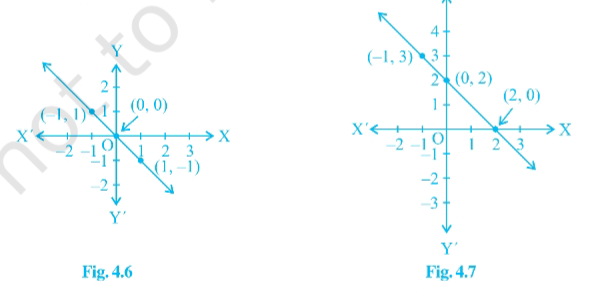
\includegraphics[width=\columnwidth]{chapters/9/figs/4.6-4.7.png}
\caption{Graph}
  \label{fig:4.6-4.7}
\end{figure}
\item If the work done by a body of a constant force is directly proportional 
to the distance travelled by the body,express this in the form of an equation
and draw the graph of the same by taking the varables and draw the graph of 
the same by taking the constant force as $5 units$.Also read from the graph the
work done when the distance travelled by the body is
\begin{enumerate}[label=(\roman*)]
\item $2$Units
\item $0$Unit
\end{enumerate}
\item Yamini and Fatima,two students of class IX of a school,together
 contributed \rupee~100 towards the prime minister's reief fund to help
 the earhquake victims.Write a linear equation which satisfies this data.
 (you may take their contributions  \rupee~x and \rupee~y.Draw the graph 
 of the same.
\item In Countries like USA and Canada temperature is measured in Celsius.
Here is a linear equation that converts Farenheit to celsius:
$F=\frac{9}{5}C+32$
\begin{enumerate}[label=(\roman*)]
\item Draw the graph of the linear equation above using Celsius for $x$
 axis and Farenheit for $y$ axis
\item If the temperature is $30\degree C$,what is the temperature in farenheight?
\item If the temperature is $95\degree F$,what is the temperature in celsius?
\item If the temperature is $0\degree C$.What is the temperature in Farenheit and if the temperature in celsius?
\item Is there a temperature Which is numerically same in both Farenheit and Celsius? If yes find it.
\end{enumerate}
\end{enumerate}

\section{10}
\subsection{Examples:-1-19 (10.3)}
\input{chapters/10/10.3.tex}
\subsection{10.3.1}
\input{chapters/10/10.3.1.tex}
\subsection{10.3.2}
\input{chapters/10/10.3.2.tex}
\subsection{10.3.3}
\begin{enumerate}
\item Solve the following pair of linear equations by the substitution method.
\begin{enumerate}[label=(\roman*)]    
	\item
	\begin{align}
   	 x+y=14 \\x-y=4
	\end{align}
    	\item 
	\begin{align}
	s-t=3
	\end{align}
	\item
	\begin{align}
    	3x-y=3\\ 9x-3y=9
	\end{align}
	\begin{align}   	
 	0.2x+0.3y=1.3\\ 0.4x+0.5y=23
	\end{align}
	\item     
	\begin{align}
	\sqrt{2x}+\sqrt{3y}=0\\ \sqrt{3x}-\sqrt{8y}=0
	\end{align}
	\item
	\begin{align}
    	\frac{3x}{2}-\frac{5y}{2}=-2\\ \frac{x}{3}+\frac{y}{2}=\frac{13}{6}
    	\end{align}
	\end{enumerate}
\item Solve $2x+3y=11$ and $2x+4y=-24$ and hence find the value of $m$ for which $y=mx+3$
\item Form the pair of linear equations for the following problems and find their solutions by the substitution method
    \begin{enumerate}[label=(\Roman*)]
    \item The difference between two numbers is $26$ and one number is three times the other. Find them.
    \item The larger of two supplementary angles exceeds the smaller by $18$ degrees. Find them.
    \item The coach of a cricket team buys $7$ balls and $6$ balls for \rupee~3800. Later, she buys $3$ bats and $5$ balls for \rupee~1750. Find the cost of each bat and each ball.
    \item The taxi charges in a city consist of a fixed charge together with the charges for the distance covered. For a distance of $10$ km, the charge paid is \rupee~105 and for a distance of $15$ km, the charge paid is \rupee~155. What are the fixed charges and the charge per km? How much does a person have to pay for travelling a distance of 25 km ? 
    \item A fraction becomes $\frac{9}{11}$ if $2$ is added to both the numerator and the denominator. If $3$ is added to both the numerator and the denominator, it becomes $\frac{5}{6}$. Find the fraction.
    \item Five years hence, the age of Jacob will be three times that of his son. Five years ago, Jacob's age was seven times that of his son. What are their present ages?
    \end{enumerate}
\end{enumerate}

\subsection{10.3.4}
\input{chapters/10/10.3.4.tex}
\subsection{10.3.5}
\input{chapters/10/10.3.5.tex}
\subsection{10.3.6}
\begin{enumerate}
\item Solve the following pair of equations by reducing them to a pair of linear equations:
\begin{enumerate}[label=(\roman*)]
\item
\begin{align}
\frac{1}{2x}+\frac{1}{3y}=2 \\ \frac{1}{3x}+\frac{1}{2y}=\frac{13}{6}
\end{align}
\item
\begin{align}
\frac{2}{\sqrt{x}}+\frac{3}{\sqrt{y}}=2\\
\frac{4}{\sqrt{x}}-\frac{9}{\sqrt{y}}=-1
\end{align}
\item
\begin{align}
\frac{4}{x}+3y=14\\ \frac{3}{x}-4y=23
\end{align}
\item
\begin{align}
\frac{5}{x-1}+\frac{1}{y-2}=2\\ \frac{6}{x-1}-\frac{3}{y-2}=1
\end{align}
\item
\begin{align}
\frac{7x-2y}{xy}=5\\ \frac{8x+7y}{xy}=15
\end{align}
\item
\begin{align}
6x+3y=6xy\\ 2x+4y=5xy
\end{align}
\item
\begin{align}
\frac{10}{x+y}+\frac{2}{x-y}=4\\ \frac{15}{x+y}-\frac{5}{x-y}=-2
\end{align}
\item
\begin{align}
\frac{1}{3x+y}+\frac{1}{3x-y}=\frac{3}{4}\\ \frac{1}{2(3x+y)}-\frac{1}{2(3x-y)}=\frac{-1}{8}
\end{align}
\end{enumerate}
\item Formulate the following problems as a pair of equations,and hence find their solutions:
\begin{enumerate}[label=(\roman*)]
\item Ritu can row downstream $20km$ in $2$ hours, and upstream $4km$ in $2$ hours. Find her speed of rowing in still water and the speed of the current.
\item $2$ women and $5$ men can together finish an embroidery work in $4$ days, while $3$ women and $6$ men can finish it in $3$ days. Find the time taken by $1$ women along to finish the work, and also that taken by $1$ men alone.
\item Roohi travels $300 km$ to her home partly by train and partly by bus. She takes $4$ hours if she travels $60km$ by train and the remaining by bus. If she travels $100km$ by train and the remaining by bus, she takes $10$ minutes longer. Find the speed of the train and the bus seperately.
\end{enumerate}
\end{enumerate}

\subsection{10.3.7}
\input{chapters/10/10.3.7.tex}
\chapter{Quadratic Equations}
\section{10}
\subsection{Examples:-1-18 (10.4)}                                               
\input{chapters/10/10.4.tex}
\subsection{10.4.1}
\input{chapters/10/10.4.1.tex}
\subsection{10.4.2}
\input{chapters/10/10.4.2.tex}
\subsection{10.4.3}
\input{chapters/10/10.4.3.tex}
\subsection{10.4.4}
\begin{enumerate}
\item Find the nature of the roots of the following quadratic equations. If real roots exist, find them:
\begin{enumerate}[label=(\roman*)]
\item $2x^2-3x+5=0$
\item $3x^2-4 sqrt 3x+4=0$
\item $2x^2-6x+3=0$
\end{enumerate}
\item Find the values of k for each of the following quadratic equations, so that they hav equal roots:
\begin{enumerate}[label=(\roman*)]
\item $2x^2=kx-3=0$
\item $kx(x-2)+6=0$
\end{enumerate}
\item Is it possible to design a rectangular mango grove whose length is twice its breadth, and the area is  $800m^2$? If so, find its length and breadth.
\item Is the following situation possible? If so, determine their present ages.
\\ The sum of the ages of the two friends is 20 years. Four years ago, the product of their ages in years was $48$.
\item Is it possible to design a rectangular park of perimeter 80m and area of $400m^2$. If so, find its length and breadth.
\end{enumerate}



\chapter{Coordinate Geometry}
\section{10}
\subsection{Examples:-1-15 (10.7)}
\input{chapters/10/10.7.tex}
\subsection{10.7.1}
\input{chapters/10/10.7.1.tex}
\subsection{10.7.2}
\input{chapters/10/10.7.2.tex}
\subsection{10.7.3}
\input{chapters/10/10.7.3.tex}
\subsection{10.7.4}
\input{chapters/10/10.7.4.tex}
\chapter{Straight Lines}
\section{11}
\subsection{Examples:-1-25 (11.10)}
\input{chapters/11/11.10.tex}
\subsection{11.10.1}
\input{chapters/11/11.10.1.tex}
\subsection{11.10.2}
\input{chapters/11/11.10.2.tex}
\subsection{11.10.3}
\input{chapters/11/11.10.3.tex}
\subsection{11.10.4}
\input{chapters/11/11.10.4.tex}
\subsection{11.11.1}
In each of the following exercise \ref{prob:1} to \ref{prob:5}, find the equation of the circle with:
\begin{enumerate}[label=\arabic*.,ref=\thesubsection.\theenumi]
\item centre $(0,2)$ and radius $2$ \label{prob:1}
\item centre $(-2,3)$ and radius $4$
\item centre $\frac({1}{2},\frac{1}{4})$ and radius $\frac {1}{!2}$
\item centre $(1,1)$ and radius $2$
\item centre $(-a,-b)$ and radius $\sqrt{a^2-b^2}$  \label{prob:5}
\end{enumerate}
In each of the following exercise \ref{prob:6} to \ref{prob:9}, find the centre and radius of the circles
\begin{enumerate}[resume]
\item $(x-5)^2+(y-3)^2=36$ \label{prob:6}
\item $x^2+y^2-4x-8y-45=0$
\item $x^2+y^2-8x+10y-12=0$
\item $2x^2+2y^2-x=0$ \label{prob:9}
\end{enumerate}
\begin{enumerate}[resume]
\item Find the equation of the circle passing through the points $(4,1)$ and $(6,5)$ and whose centre is on the line $4x+y=16$.
\item Find the equation of the circle passing through the points $(2,3)$ and $(-1,1)$ and whose centre is on the line $x-3y-11=0$.
\item Find the equation of the circle with radius 5 whose centre lies on x-axis and passes through the point $(2,3)$.
\item Find the equation of the circle passing through $(0,0)$ and making intercepts $a$ and $b$ on the coordinate axes.
\item Find the equation of a circle with centre $(2,2)$ and passes through the point $(4,5)$.
\item Does the point $(-2.5,3.5)$ lie inside, outside or on the circle $x^2+y^2=25$.
\end{enumerate}



\subsection{11.12.1}
\input{chapters/11/11.12.1.tex}
\subsection{11.12.2}
\input{chapters/11/11.12.2.tex}
\subsection{11.12.3}
\input{chapters/11/11.12.3.tex}
\subsection{11.12.4}
\begin{enumerate}
\item Three vertices of a parallelogram $ABCD$ are $A(3,-1,2), B(1,-2,4)$ and $C(-1,1,2)$. Find the coordinates of the fourth vertex.
\item Find the lengths of the medians of the triangle with vertice $A(0,0,6), B(0,4,0)$ and $(6,0,0)$.
\item If the origin is the centroid of the triangle $PQR$ with vertices $P(2a,2,6), Q(-4,3b,-10)$ and $R(8,14,2c)$, then find the values of $a, b$ and $c$.
\item Find the coordinates of a point on y-axis which are at a distance of $5\sqrt2$ from the point $P(3,-2,5)$.
\item A point $R$ with x-coordinate $4$ lies on the line segment joining the points $P(2,-3,4)$ and $Q(,0,10)$. Find the coordinates of the point $R$.
\item If $A$ and $B$ be the points $(3,4,5)$ and $(-1,3,-7)$ respectively, find the equation of the set of the points $P$ such that $PA^2+PB^2=K^2$ where $K$ is a constant.
\end{enumerate}
  

\chapter{Trigonometry}
\section{Ratios}
\input{./chapters/trig/tri_geo_rt}
\section{The Baudhayana Theorem}
\input{./chapters/trig/tri_geo_baudh}
%
\section{Area of a Triangle}
\input{./chapters/trig/tri_geo_sincos}
\section{Angle Bisectors}
\input{./chapters/trig/ang.tex}
\section{Circumradius}
\input{./chapters/trig/tri_geo_cradius}
\section{Tangent}
\input{./chapters/trig/tangent}
\section{Identities}
\input{./chapters/trig/trig_id.tex}
\chapter{Analytic Geometry}
\section{Vectors}
\input{./chapters/coord/vector}
\section{Altitudes of a Triangle:Line Equation}
\input{./chapters/coord/tri_geo_alt}
\section{Circumcircle: Circle Equation}
\input{./chapters/coord/tri_geo_ccentre}
\section{Tangent}
\input{./chapters/coord/circ_geo_prop}
\chapter{Triangle}
\input{./chapters/exercises/tri_geo_exer}
\chapter{Quadrilateral}
\input{./chapters/exercises/quad_geo_exer}
%
\chapter{Circle}
\input{./chapters/exercises/circ_geo_exer}
\chapter{Miscellaneous }
\input{./chapters/exercises/geo_misc}
\iffalse
%\include{ch02} 
\backmatter
\appendix
\chapter{Area of a Circle}
\input{./chapters/area/circ_geo_area}
\fi
%
%\chapter{Proofs}
%   \section{}
%\input{apps/defs.tex}

%  \section{}
%\input{apps/parab.tex}
%  \section{}
%\input{apps/nonparab.tex}
%		\section{}
%\input{apps/params.tex}
\latexprintindex

\end{document}

 
